% Options for packages loaded elsewhere
\PassOptionsToPackage{unicode}{hyperref}
\PassOptionsToPackage{hyphens}{url}
%
\documentclass[
  11pt,
  a4paper,
  openany]{book}
\usepackage{amsmath,amssymb}
\usepackage{amsthm}
\usepackage{tikz}
\theoremstyle{definition}
\newtheorem{proposition}{Proposition}[chapter]
% Compteur commun des résultats formels, remis à zéro à chaque chapitre.
% Ces deux commandes conservent la mise en page existante tout en rendant
% les résultats numérotés et référencables de façon stable.
\newcommand{\resultheading}[3]{%
  \refstepcounter{proposition}\label{#2}%
  \textbf{#1~\theproposition#3.}%
}
\newcommand{\resultstep}[1]{\refstepcounter{proposition}\label{#1}}
\renewcommand{\proofname}{Démonstration}
\usepackage[numbers,sort&compress]{natbib}
\usepackage{longtable,booktabs,array,calc}
\usepackage{float}
\usepackage[T1]{fontenc}
\usepackage[utf8]{inputenc}
\usepackage{textcomp} % provide euro and other symbols
\usepackage{lmodern}
\usepackage{appendix}
\usepackage[]{microtype}
\UseMicrotypeSet[protrusion]{basicmath} % disable protrusion for tt fonts
\usepackage{parskip}
\usepackage{xcolor}
\usepackage[hidelinks]{hyperref}
\usepackage[margin=2.7cm]{geometry}
\usepackage[most]{tcolorbox}
\tcbset{
  enhanced,
  breakable,
  colback=white,
  colframe=black!15,
  arc=2mm,
  boxrule=0.5pt,
  left=2mm,right=2mm,top=1.5mm,bottom=1.5mm
}
\newcommand{\planche}[4]{%
  \begin{center}\includegraphics[height=#1]{#2}\end{center}
  \vspace{-0.15cm}
  {\small\textsc{#3}}\\[0.10cm]
  {\footnotesize #4}
  \vspace{0.55cm}
}
\makeatletter

\providecommand*{\toclevel@tome}{-2}%
\newcommand{\l@tome}[2]{%
  \addpenalty{-\@highpenalty}%
  \vskip 1.5em
  \@tempdima 1.5em
  \begingroup
    \parindent \z@
    \rightskip \@pnumwidth
    \parfillskip -\@pnumwidth
    \leavevmode
    \bfseries
    \advance\leftskip\@tempdima
    \hskip -\leftskip
    #1\nobreak\hfill
    \nobreak\hb@xt@\@pnumwidth{\hss #2}\par
  \endgroup
}

\makeatother

\newcounter{tome}
\AtBeginDocument{%
  \renewcommand*{\theHpart}{\arabic{tome}.\arabic{part}}%
}

\newcommand{\tome}[2]{%
  \cleardoublepage

  \stepcounter{tome}%
  \setcounter{part}{0}%

  \phantomsection
  \addcontentsline{toc}{tome}{Tome #1 --- #2}

  \thispagestyle{empty}
  \begin{center}
    \vspace*{\fill}
    {\Large\scshape Tome #1\par}
    \vspace{1.5cm}
    {\Huge\bfseries #2\par}
    \vspace*{\fill}
  \end{center}

  \cleardoublepage
}
% Régimes explicités
\newtcolorbox{encadre}[1][]{title=Note,#1}
\setlength{\emergencystretch}{3em} % prevent overfull lines
\providecommand{\tightlist}{%
  \setlength{\itemsep}{0pt}\setlength{\parskip}{0pt}}
\setcounter{secnumdepth}{3}
\usepackage[bidi=default]{babel}
\babelprovide[main,import]{french}
\let\LanguageShortHands\languageshorthands
\def\languageshorthands#1{}
\usepackage{iftex}
\ifLuaTeX
  \usepackage{selnolig} % suppression des ligatures réservée à LuaLaTeX
\fi
\usepackage{bookmark}
\usepackage{xurl}
\urlstyle{same}
\title{IWS}
\usepackage{etoolbox}
\makeatletter
\providecommand{\subtitle}[1]{% add subtitle to \maketitle
  \apptocmd{\@title}{\par {\large #1 \par}}{}{}
}
\makeatother
\subtitle{Noyau hybride, système ouvert, interface et histoires}
\author{BadH}
\date{septembre 2026}

\begin{document}
\frontmatter
\maketitle

{
\setcounter{tocdepth}{1}
\tableofcontents
}
\mainmatter

\chapter*{Avant-propos}
\addcontentsline{toc}{chapter}{Avant-propos}

IWS signifie \emph{Inner World System}.

Ce nom désigne ici une classe de systèmes dynamiques dont l'état présent ne suffit pas nécessairement à déterminer, à lui seul, la manière dont ils répondront à ce qui leur arrive ensuite. Leur histoire peut modifier leur dynamique, leur structure, leur interface ou l'accessibilité de leurs réponses futures.

Le terme \emph{inner world} ne désigne pas un monde intérieur au sens psychologique, phénoménologique ou métaphysique. Il désigne l'organisation interne par laquelle le système reçoit, transforme et conserve certains effets de ce qu'il traverse. Les mots \emph{trace}, \emph{mémoire}, \emph{résistance}, \emph{appropriation} ou \emph{histoire} sont employés dans le même esprit : chacun reçoit dans le texte une définition fonctionnelle ou mathématique et ne doit pas être chargé d'une interprétation supplémentaire.

Ce volume construit un cadre minimal pour étudier cette dépendance à l'histoire.

Le premier tome définit un noyau dynamique hybride dans lequel une trace modifie l'évolution future et des événements discrets peuvent transformer la structure relationnelle. Le deuxième ouvre ce noyau à une interaction et étudie comment une interface peut filtrer, accumuler ou conserver les effets d'une exposition. Le troisième déplace enfin la question vers l'observation : deux réalisations sont comparées non par ce que l'on suppose de leur intérieur, mais par les réponses que des sondes déclarées permettent effectivement de distinguer.

Cette progression ne constitue pas une théorie générale de la mémoire, de l'apprentissage, de la cognition ou de l'individuation. Elle ne suppose pas non plus que le système poursuive un objectif, optimise une fonction ou possède une représentation de son propre passé. Le cadre cherche plus modestement à isoler des mécanismes par lesquels une dynamique peut dépendre de ce qu'elle a traversé, puis à préciser ce qu'un observateur peut légitimement inférer de cette dépendance.

Le document distingue pour cette raison plusieurs niveaux d'affirmation. Définitions, choix de modélisation, résultats démontrés, résultats conditionnels, observations numériques, conjectures et interprétations ne possèdent pas le même statut. Les marques utilisées dans le texte rendent ces différences explicites. Les annexes rassemblent les démonstrations, développements analytiques et protocoles numériques nécessaires lorsque leur détail interromprait la lecture du corps principal.

Les affirmations doivent être lues relativement aux hypothèses qui les accompagnent. Un résultat analytique est mis en défaut par un contre-exemple satisfaisant ses hypothèses. Un résultat numérique est mis en défaut si le protocole déclaré, reproduit dans les mêmes conditions, ne produit pas le phénomène annoncé. Une interprétation n'acquiert pas le statut d'un résultat parce qu'elle est compatible avec lui. Inversement, l'échec d'une propriété dans un régime qui n'entre pas dans ses hypothèses ne réfute pas l'énoncé qui a effectivement été établi.

Cette discipline est particulièrement importante ici parce que le vocabulaire utilisé est volontairement évocateur. Le modèle peut montrer qu'une trace modifie un futur sans montrer qu'un système \emph{se souvient} au sens usuel ; qu'une interaction laisse une transformation persistante sans établir un apprentissage ; ou que deux réalisations sont séparables par leurs réponses sans permettre de reconstruire ce qui les distingue intérieurement.

Le cadre proposé doit donc être lu à deux niveaux simultanément : comme un système dynamique concret, dont les équations et les expériences peuvent être examinées, et comme un dispositif de distinction entre ce qui est démontré, ce qui est observé et ce qui est seulement suggéré par ces résultats.

C'est dans cette limite que le terme \emph{Inner World System} prend son sens dans ce volume : non comme la désignation d'un intérieur que l'on prétendrait connaître, mais comme celle d'un système dont les traversées passées peuvent modifier les conditions de ses réponses futures.

\chapter*{Positionnement bibliographique}
\addcontentsline{toc}{chapter}{Positionnement bibliographique}
IWS n’introduit pas dans un vide théorique les objets mathématiques qu’il mobilise. Son noyau relève explicitement de la famille des systèmes dynamiques hybrides et emprunte à des outils classiques de dynamique différentielle, de systèmes impulsifs et de théorie des bifurcations déjà référencés dans le présent volume.  Le positionnement qui demande davantage de précision concerne surtout le Tome III : la dépendance à l’histoire, les équivalences définies par les réponses futures, les quotients d’observation et la structure hiérarchique obtenue à partir de la séparabilité. Il ne s’agit pas ici de revendiquer comme nouveaux ces outils pris séparément, mais de préciser les traditions avec lesquelles leur usage dans IWS dialogue.

La dépendance du comportement présent à l’histoire possède notamment une longue tradition dans la théorie mathématique de l’hystérésis. Les travaux de Krasnosel’skiĭ et Pokrovskiĭ étudient systématiquement des systèmes dont la réponse porte des effets de mémoire et d’irréversibilité, tandis que Mayergoyz développe des modèles où la mémoire du passé est sélective : toute l’histoire de l’entrée n’a pas à demeurer active pour influencer les états futurs \cite{krasnoselskii1989systems,mayergoyz1991mathematical}. Ce voisinage est important pour IWS, mais il ne constitue pas une identification. La dépendance à l’histoire n’y est pas ramenée à un opérateur d’hystérésis entrée–sortie. Elle peut être portée par la trace, par un état lent de l’interface ou par l’ordre de transformations discrètes ; elle peut modifier la dynamique ultérieure, l’accessibilité de certaines réponses ou la structure elle-même. De plus, ce qui survit d’une histoire n’est pas supposé en constituer une archive : une différence passée importe seulement tant qu’elle reste capable d’affecter des réponses futures. 

Un second voisinage est celui des \textbf{équivalences comportementales}. La bisimulation et la coinduction fournissent une tradition générale pour comparer des systèmes par leurs comportements plutôt que par l’identité de leur représentation interne ; la formulation coalgébrique de Rutten étend notamment ce point de vue à diverses classes de systèmes de transition et de systèmes dynamiques \cite{rutten2000universal,sangiorgi2011bisimulation}. IWS ne prétend cependant pas que son équivalence en réponse soit une bisimulation au sens usuel. Pour une classe d’histoires admissibles \(\mathfrak B\) et une résolution de lecture \(\rho\), deux systèmes y sont déclarés équivalents lorsque leurs cartes de réponse coïncident sur \(\mathfrak B\). Cette équivalence est donc explicitement relative aux expériences autorisées et à ce que l’observateur choisit de lire : elle affirme une indiscernabilité dans un protocole déclaré, non une identité des systèmes comparés. 

Lorsque toutes les continuations admissibles sont disponibles, cette construction rejoint plus précisément la tradition de Nerode. L’idée de regrouper des états qu’aucun futur ne permet de distinguer est classique dans la théorie des automates \cite{nerode1958linear}. Dans IWS, le même principe apparaît au niveau des histoires : sur le monoïde complet des continuations, l’équivalence en réponse est stable par préfixage et définit une congruence comportementale. Le manuscrit réserve pour cette raison le terme de \textit{quotient de Nerode} à ce cas complet. Les classes limitées par un budget expérimental restent, elles, de simples quotients d’observation : elles peuvent être raffinées lorsque l’on enrichit les histoires admissibles ou la résolution de lecture.  Cette distinction évite en particulier de transposer sans précaution au cadre d’IWS les résultats de minimalité propres aux automates finis.

Le passage d’une équivalence binaire à une comparaison quantitative possède lui aussi des antécédents. Des pseudométriques comportementales ont été construites afin de mesurer à quel degré deux systèmes diffèrent, notamment pour des systèmes de transition probabilistes \cite{vanbreugel2005behavioural}. La quantité introduite dans IWS répond cependant à une question différente. Elle ne mesure ni une distance physique entre états ni l’écart probabiliste entre leurs transitions : elle mesure la \textbf{complexité minimale d’une histoire capable de séparer leurs réponses}. La profondeur ainsi obtenue satisfait une inégalité forte ; après une transformation décroissante, elle définit une pseudo-ultramétrique sur les systèmes et une ultramétrique sur leur quotient d’observation. La construction ne requiert à ce niveau ni représentation vectorielle commune, ni concaténation des histoires, ni caractère binaire des réponses. 

La structure hiérarchique qui en résulte n’est pas non plus spécifique à IWS. La correspondance entre ultramétriques, familles de partitions emboîtées et représentations dendrogrammatiques est classique ; Carlsson et Mémoli en donnent notamment une formulation explicite dans leur étude des méthodes de classification hiérarchique \cite{carlsson2010characterization}. IWS n’en déduit pas une méthode de \textit{clustering}. Le dendrogramme sert seulement à représenter la filtration des classes d’indiscernabilité lorsque l’on augmente la complexité des histoires disponibles. Sa hauteur n’exprime ni une proximité d’état, ni une généalogie, ni une similarité intrinsèque de mécanisme : elle indique jusqu’à quelle profondeur expérimentale deux systèmes restent interchangeables pour l’observateur déclaré. Cette restriction est explicite dans l’Annexe L. 

La spécificité d’IWS se situe donc moins dans chacune de ces constructions que dans \textbf{leur mise en continuité dans un même cadre}. Une dynamique hybride porte des modifications héritées de l’histoire ; des histoires supplémentaires peuvent ensuite être utilisées comme expériences et comme sondes ; leurs réponses définissent des équivalences relatives ; certaines histoires peuvent être comprimées dans un contenu survivant ou dans un résumé lent suffisant ; les réponses organisent des frontières observables ; enfin, la complexité minimale nécessaire pour rompre une équivalence munit le quotient correspondant d’une géométrie hiérarchique. Le Tome III organise précisément cette chaîne, des histoires et des réponses jusqu’à la séparabilité ultramétrique. 

Cette articulation fixe également la portée des revendications. IWS ne propose ni une nouvelle théorie générale de l’hystérésis, ni une nouvelle théorie de la bisimulation, ni une généralisation de la théorie des automates, ni une méthode de classification hiérarchique. Il ne suppose pas davantage que les comportements observables permettent de reconstruire un mécanisme interne unique. La dépendance à l’histoire n’établit à elle seule ni apprentissage ni finalité, et l’équivalence demeure relative aux histoires et aux lectures effectivement déclarées. Ces limitations sont cohérentes avec la discipline suivie dans le reste du volume : les objets introduits servent à formuler des propriétés testables du cadre étudié, non à leur attribuer une interprétation plus large que ce que les résultats permettent. 


\tome{I}{Le noyau hybride}
\hspace{0pt}
\vfill
\planche{10.6cm}{fig/planche_I_sillon.pdf}
{Tome I — Le sillon}
{Les retours vers le repos, marqués à intervalles de temps égaux. Là où le
système est déjà passé, le retour s'attarde~: les marques se resserrent et
l'encre se dépose. Ailleurs, rien n'a changé, et aucune direction n'est renforcée.}
\vfill
\hspace{0pt}
\newpage
\chapter*{Statut du document}\label{statut-document}
\addcontentsline{toc}{chapter}{Statut du document}

La première partie présente le noyau mathématique retenu pour IWS. Elle reprend la \emph{Core Specification} 0.1 en intégrant les corrections de la version 0.1.1. Elle ne retrace pas la succession des corrections : elle expose directement le modèle qui en résulte.

Le but de cette première partie est limité : définir les variables, les équations continues, les événements de Kairos et les propriétés déjà établies. La réduction homogène utilisée dans le Tome II est rappelée à la fin de la partie.

Lorsqu'une étiquette de statut est utilisée dans le corps du texte ou dans les synthèses numériques, elle a le sens indiqué ci-dessous. Cette taxonomie qualifie des définitions, des choix de modélisation, des résultats ou des contrôles ; elle n'est pas apposée systématiquement aux résultats formels des annexes. Dans celles-ci, le type de l'énoncé (définition, lemme, proposition, théorème ou corollaire), ses hypothèses et sa démonstration fixent directement son statut. L'absence d'étiquette dans une annexe ne signifie donc pas que le statut de l'énoncé est indéterminé.

\begin{itemize}
\tightlist
\item
  \texttt{{[}DEF{]}} : définition ;
\item
  \texttt{{[}CHOIX{]}} : choix de modélisation ;
\item
  \texttt{{[}PROP{]}} : résultat démontré ;
\item
  \texttt{{[}PROP-COND{]}} : résultat démontré sous des conditions
  explicites ;
\item
  \texttt{{[}PROP-NUM{]}} : résultat analytique complété ou contrôlé
  numériquement ;
\item
  \texttt{{[}NUM{]}} : fait observé dans le protocole indiqué ;
\item
  \texttt{{[}CTRL{]}} : expérience de contrôle construite pour écarter une interprétation concurrente d'un résultat numérique ;
\item
  \texttt{{[}OUVERT{]}} : question non résolue ;
\item
  \texttt{{[}CONJ{]}} : conjecture ;
\item
  \texttt{{[}INTERP{]}} : interprétation du résultat, distincte de sa
  démonstration.
\end{itemize}

\chapter{Question traitée}\label{t1-question-traitee}

IWS cherche à représenter un système dont le comportement présent dépend de son histoire, sans réduire cette histoire à un paramètre fixé une fois pour toutes.

Le noyau repose sur trois idées.

Premièrement, chaque nœud possède un état rapide \(H_i\) et une vitesse \(V_i\). La dynamique n'est donc pas un simple déplacement instantané dans l'espace des états : elle comporte une inertie minimale.

Deuxièmement, chaque nœud possède une trace \(\tau_i\). Cette trace porte une mémoire dissipative et modifie le rappel ainsi que la dissipation. Deux nœuds qui ont les mêmes valeurs de \(H_i\) et \(V_i\) peuvent donc évoluer différemment s'ils n'ont pas la même trace.

Troisièmement, le graphe relationnel ne varie pas continûment. Il change lors d'événements discrets, appelés \textbf{Kairos}, déclenchés lorsqu'une pression locale atteint un seuil.

Le modèle mêle ainsi une dynamique différentielle et des changements discrets. Il appartient à la famille des systèmes dynamiques hybrides \cite{goebel2012hybrid, lakshmikantham1989impulsive}.

Cette classification n'est pas une interprétation. Elle décrit simplement la forme mathématique du système :

\[
(\mathcal X,C,F,D,\mathcal K).
\]

Dans cette écriture :

\begin{itemize}
\tightlist
\item
  \(\mathcal X\) est l'espace des états ;
\item
  \(C\) est l'ensemble dans lequel la dynamique continue est autorisée ;
\item
  \(F\) désigne le champ de vecteurs suivi entre deux événements ;
\item
  \(D\) est l'ensemble dans lequel un saut doit être effectué ;
\item
  \(\mathcal K\) décrit l'effet de ce saut.
\end{itemize}

\chapter{État du système}\label{t1-etat-du-systeme}

\section{Graphe et dimensions}\label{t1-graphe-et-dimensions}

Le nombre de nœuds \(N\geq 2\) est fixe dans le noyau. La dimension de l'état interne est \(d\geq 1\).

On note

\[
\mathcal V=\{1,\ldots,N\}
\]

l'ensemble des nœuds. Le graphe est simple, non orienté et sans boucle. Sa matrice d'adjacence est

\[
A\in\{0,1\}^{N\times N},
\qquad
A^\top=A,
\qquad
A_{ii}=0.
\]

Le nombre de nœuds ne varie donc pas dans ce chapitre. Les mécanismes de suppression ou de création de nœuds appartiennent à des extensions ultérieures.

\section{Variables nodales}\label{t1-variables-nodales}

Chaque nœud \(i\) porte quatre variables :

\[
H_i\in\mathbb R^d,
\qquad
V_i\in\mathbb R^d,
\qquad
\tau_i\in\mathbb R^d,
\qquad
P_i\in\mathbb R_+.
\]

Leur rôle est le suivant.

\subsection{État rapide \texorpdfstring{\(H_i\)}{Hi}}\label{t1-etat-rapide-h_i}

\(H_i\) décrit la configuration instantanée du nœud. Le modèle ne lui attribue pas, à ce stade, de contenu symbolique particulier. Selon l'application envisagée, ses composantes pourraient représenter des grandeurs différentes. Le noyau exige seulement qu'elles appartiennent à un espace vectoriel de dimension finie.

\subsection{Vitesse \texorpdfstring{\(V_i\)}{Vi}}\label{t1-vitesse-v_i}

La relation

\[
\dot H_i=V_i
\]

introduit une dynamique d'ordre deux. \(V_i\) ne représente pas nécessairement une vitesse physique. Il mesure la variation en cours de l'état et permet de distinguer deux nœuds qui se trouvent au même point \(H_i\), mais qui n'y arrivent pas avec la même dynamique.

\subsection{Trace \texorpdfstring{\(\tau_i\)}{tau i}}\label{t1-trace-tau_i}

La trace est la variable historique du noyau. Elle est alimentée par l'état relationnel reçu par le nœud et décroît en l'absence de nouvelle écriture. Elle intervient ensuite dans deux termes de la dynamique :

\begin{itemize}
\tightlist
\item
  la friction \(\Gamma(\tau_i)\) ;
\item
  le préconditionneur \(M(\tau_i)\).
\end{itemize}

La trace ne pousse donc pas directement \(H_i\). Elle modifie la dissipation et le terme de rappel vers l’origine.

\subsection{Pression \texorpdfstring{\(P_i\)}{Pi}}\label{t1-pression-p_i}

\(P_i\) est un accumulateur local utilisé pour déclencher les Kairos. Le mot « pression » ne désigne pas une pression physique. Il résume ici une combinaison de l'amplitude de l'état, de la vitesse et d'une relaxation.

\begin{encadre}
L'état complet est

\[
x=(H,V,\tau,P,A)
\]

et l'espace des états est

\[
\mathcal X
=
\mathbb R^{N\times d}
\times
\mathbb R^{N\times d}
\times
\mathbb R^{N\times d}
\times
\mathbb R_+^N
\times
\mathfrak G_N,
\]

où \(\mathfrak G_N\) désigne l'ensemble des graphes simples non orientés
sur \(\mathcal V\).
\end{encadre}

\chapter{Influence du graphe}\label{t1-influence-du-graphe}

\section{Matrice relationnelle
normalisée}\label{t1-matrice-relationnelle-normalisee}

Les interactions entre nœuds passent par la matrice

\[
\widetilde A(A)
=
\operatorname{Deg}(A+I)^{-1}(A+I),
\]

avec

\[
\operatorname{Deg}(B)
=
\operatorname{diag}\!\left(\sum_j B_{ij}\right).
\]

L'ajout de \(I\) donne à chaque nœud une boucle de calcul, même si le graphe est vide. La matrice \(\widetilde A\) est stochastique par lignes :

\[
\sum_j \widetilde A_{ij}=1,
\qquad
\widetilde A_{ij}\geq 0.
\]

Par conséquent,

\[
(\widetilde A H)_i
=
\sum_j \widetilde A_{ij}H_j
\]

est une moyenne pondérée de l'état du nœud et de celui de ses voisins. On dispose immédiatement de la borne

\[
\|(\widetilde A H)_i\|
\leq
\max_j \|H_j\|.
\]

Cette propriété sera utile pour l'existence des solutions et pour la borne sur la trace.

\section{Ce que le couplage ne fait pas}\label{t1-ce-que-le-couplage-ne-fait-pas}

Le couplage relationnel ne transmet ni la trace \(\tau_j\), ni la pression \(P_j\), ni les paramètres internes du voisin. Il ne transmet que les états \(H_j\) à travers leur moyenne normalisée.

Cette distinction est importante : dans le noyau, l'histoire d'un nœud n'est pas copiée dans un autre nœud. Elle n'agit sur les voisins qu'indirectement, par les effets qu'elle produit sur l'état \(H_i\).

\chapter{Trace et préconditionneur}\label{t1-trace-et-preconditionneur}

\section{Écriture de la trace}\label{t1-ecriture-de-la-trace}

La trace suit l'équation

\[
\dot\tau_i
=
\alpha\,\tanh\!\bigl((\widetilde A H)_i\bigr)
-
\beta\tau_i,
\qquad
\alpha>0,
\quad
\beta>0,
\]

où \(\tanh\) est appliquée composante par composante.

Le premier terme écrit dans la trace une version saturée de l'état relationnel. Le second terme produit un oubli exponentiel.

Le choix de \(\tanh\) a une conséquence mathématique immédiate :

\[
\left\|
\tanh\!\bigl((\widetilde A H)_i\bigr)
\right\|
\leq \sqrt d.
\]

On en déduit, presque partout,

\[
\frac{\mathrm d}{\mathrm dt}\|\tau_i\|
\leq
\alpha\sqrt d-\beta\|\tau_i\|.
\]

Ainsi,

\[
\|\tau_i(t)\|
\leq
\max\left(
\|\tau_i(0)\|,
\frac{\alpha\sqrt d}{\beta}
\right)
:=\bar\tau_i.
\]

La trace est donc bornée indépendamment de \(H\).

Cette saturation est un choix de modélisation, pas une nécessité générale démontrée. Avec une trace linéaire,

\[
\dot\tau_i=\alpha(\widetilde A H)_i-\beta\tau_i,
\]

une preuve conjointe que \(H\) et \(\tau\) restent bornés demeure possible en principe. Elle n'est simplement pas disponible dans l'analyse actuelle. La saturation est retenue parce qu'elle donne une borne autonome sur \(\tau\) et simplifie les preuves qui suivent.

\section{Matrice \texorpdfstring{\(Q(\tau)\)}{Q(tau)}}\label{t1-matrice-qtau}

La trace modifie le rappel par la matrice

\[
Q(\tau)
=
I_d+
\frac{\lambda}{1+\|\tau\|^2}\tau\tau^\top,
\qquad
\lambda\geq 0.
\]

Il s'agit d'une perturbation de rang un de l'identité. Dans toute direction orthogonale à \(\tau\), \(Q(\tau)\) agit comme l'identité. Dans la direction de \(\tau\), sa valeur propre est

\[
1+\frac{\lambda\|\tau\|^2}{1+\|\tau\|^2}.
\]

Elle vaut \(1\) si \(\lambda=0\) et appartient à \([1,1+\lambda)\) si \(\lambda>0\).

Le noyau n'utilise pas directement \(Q\), mais son inverse

\[
M(\tau)=Q(\tau)^{-1}.
\]

\section{Calcul de \texorpdfstring{\(M(\tau)\)}{M(tau)}}\label{t1-calcul-de-mtau}

La formule de Sherman--Morrison donne l'inverse d'une matrice modifiée
par un terme de rang un \cite{sherman1950adjustment}. Pour

\[
Q=I+c\,\tau\tau^\top,
\qquad
c=\frac{\lambda}{1+\|\tau\|^2},
\]

elle s'écrit

\[
Q^{-1}
=
I-
\frac{c}{1+c\,\tau^\top\tau}
\tau\tau^\top.
\]

Le terme \(\tau^\top\tau\) est bien présent. Comme

\[
\tau^\top\tau=\|\tau\|^2,
\]

on obtient

\[
\frac{c}{1+c\|\tau\|^2}
=
\frac{
\dfrac{\lambda}{1+\|\tau\|^2}
}{
1+
\dfrac{\lambda\|\tau\|^2}{1+\|\tau\|^2}
}
=
\frac{\lambda}
{1+(1+\lambda)\|\tau\|^2}.
\]

Par conséquent,

\[
\boxed{
M(\tau)
=
I_d
-
\frac{\lambda}
{1+(1+\lambda)\|\tau\|^2}
\tau\tau^\top
}.
\]

Cette forme permet de lire directement son action.

Dans les directions orthogonales à \(\tau\), \(M(\tau)z=z\).

Dans la direction de \(\tau\), la valeur propre est
\(
m_\parallel(\tau)
=
\frac{1+\|\tau\|^2}
{1+(1+\lambda)\|\tau\|^2}.
\)

Elle décroît de \(1\) vers \(m_0=\frac{1}{1+\lambda}\) lorsque \(\|\tau\|\) augmente.

Le terme \(-M(\tau_i)H_i\) rappelle donc \(H_i\) vers l'origine, mais ce rappel est plus faible dans la direction de la trace. Les directions orthogonales ne sont pas renforcées : elles restent inchangées.

Pour cette raison, \(M\) est appelé \textbf{préconditionneur anisotrope historique}. Le mot « métrique » n'est pas employé dans les énoncés mathématiques : la dynamique ne contient pas les termes qu'exigerait une véritable formulation riemannienne.

\section{Friction dépendant de la trace}\label{t1-friction-dependant-de-la-trace}

La friction est :

\[
\Gamma(\tau)
=
\gamma_0+\gamma_1\|\tau\|,
\qquad
\gamma_0>0,
\quad
\gamma_1\geq 0.
\]

Elle augmente avec la norme de la trace. La trace a donc deux effets distincts :

\begin{itemize}
\tightlist
\item
  elle affaiblit le rappel dans sa propre direction ;
\item
  elle augmente la dissipation du mouvement.
\end{itemize}

\(M\) est lisse. En revanche, \(\Gamma\) n'est pas différentiable en \(\tau=0\), car la norme euclidienne ne l'est pas. Elle est toutefois globalement lipschitzienne, ce qui suffit pour l'existence et l'unicité des solutions.

\chapter{Dynamique continue}\label{t1-dynamique-continue}

\section{Équations}\label{t1-equations}

Entre deux Kairos, le graphe reste constant et chaque nœud suit

\[
\dot H_i=V_i,
\]

\[
\dot V_i
=
-\Gamma(\tau_i)V_i
-
M(\tau_i)H_i
+
\zeta\,\tanh\!\bigl((\widetilde A H)_i\bigr)
+
u_i(t),
\]

\[
\dot\tau_i
=
\alpha\,\tanh\!\bigl((\widetilde A H)_i\bigr)
-
\beta\tau_i,
\]

\[
\dot P_i
=
\kappa_1\|H_i\|
+
\kappa_2\|V_i\|
-
\kappa_3P_i,
\]

\[
\dot A=0.
\]

L'entrée \(u_i(t)\) est exogène, mesurable et bornée :

\[
\|u_i(t)\|\leq u_{\max}.
\]

Le cas autonome correspond à \(u\equiv 0\). Un bruit ou un forçage hétérogène particulier peut être introduit par \(u\), mais il ne fait pas partie du mécanisme interne du noyau.

\section{Lecture terme par terme}\label{t1-lecture-terme-par-terme}

L'équation de \(V_i\) contient quatre contributions.

\subsection{Dissipation}\label{t1-dissipation}

\[
-\Gamma(\tau_i)V_i
\]

freine le mouvement. La dissipation minimale vaut \(\gamma_0\). Elle augmente avec la trace lorsque \(\gamma_1>0\).

\subsection{Rappel}\label{t1-rappel}

\[
-M(\tau_i)H_i
\]

ramène l'état vers l'origine. Ce rappel est anisotrope : il est moins fort dans la direction de \(\tau_i\).

\subsection{Couplage relationnel}\label{t1-couplage-relationnel}


\[
\zeta\,\tanh\!\bigl((\widetilde A H)_i\bigr)
\]

fait dépendre la dynamique de l'état moyen du voisinage. La saturation borne ce terme par \(\zeta\sqrt d\).

\subsection{Entrée extérieure}\label{t1-entree-exterieure}

\[
u_i(t)
\]

permet d'étudier une sollicitation, un bruit imposé ou, plus tard, une interaction passant par une interface. Le noyau ne suppose pas que cette entrée soit optimisée ou porte une récompense.

\section{Pression de Kairos}\label{t1-pression-de-kairos}

La pression vérifie une équation linéaire forcée :

\[
\dot P_i
=
\kappa_1\|H_i\|
+
\kappa_2\|V_i\|
-
\kappa_3P_i.
\]

Elle est alimentée par l'amplitude de l'état et de la vitesse et possède un terme de relaxation \(-\kappa_3P_i\).

La pression n'agit pas sur la dynamique de \(H_i\), \(V_i\) ou \(\tau_i\) entre deux événements. Son seul rôle dans le noyau est de déterminer quand un Kairos doit avoir lieu.

\chapter{Déclenchement et effet des Kairos}\label{t1-declenchement-et-effet-des-kairos}

\section{Ensemble de flot et ensemble de saut}\label{t1-ensemble-de-flot-et-ensemble-de-saut}

On fixe un seuil \(\Theta>0\).

La dynamique continue est suivie tant que

\[
P_i\leq\Theta
\qquad
\text{pour tout }i.
\]

L'ensemble correspondant est

\[
C
=
\{x\in\mathcal X:\ P_i\leq\Theta\ \forall i\}.
\]

Un saut doit être effectué dès qu'au moins une pression atteint le seuil
:

\[
D
=
\{x\in\mathcal X:\ \exists i,\ P_i\geq\Theta\}.
\]

Sur la frontière \(C\cap D\), le saut est prioritaire. Comme \(P_i(t)\) est continu pendant le flot, un premier franchissement se produit avec \(P_i=\Theta\).

Le terme anglais \emph{guard} est fréquent dans la littérature sur les systèmes hybrides. Nous utilisons ici « condition de déclenchement » ou « ensemble de saut », qui suffisent à décrire le modèle.

\section{Opérateurs nodaux}\label{t1-operateurs-nodaux}

Pour chaque nœud \(i\), on définit un opérateur de Kairos

\[
\mathcal{K}_i:\mathcal D_i\longrightarrow\mathcal X,
\qquad
\mathcal D_i=\{x:\ P_i\geq\Theta\}.
\]

L'application effectivement utilisée par le noyau choisit le plus petit indice parmi les nœuds au-dessus du seuil :

\[
\iota(x)
=
\min\{i:\ P_i\geq\Theta\},
\qquad
\mathcal{K}(x)
=
\mathcal{K}_{\iota(x)}(x).
\]

Ce départage rend le modèle déterministe à entrée donnée.

\section{Recâblage conservatif}\label{t1-recablage-conservatif}

Soit \(i^\ast\) le nœud sélectionné. On note \(\mathcal N(i^\ast)\) son voisinage et \(\mathcal N^c(i^\ast)\) l'ensemble de ses non-voisins, en excluant \(i^\ast\).

La similarité entre deux traces est

\[
s(i,j)
=
\frac{\langle\tau_i,\tau_j\rangle}
{\|\tau_i\|\,\|\tau_j\|}
\]

lorsque les deux normes sont non nulles, et \(s(i,j)=0\) sinon.

Le nombre d'arêtes modifiées est

\[
m
=
\min\bigl(
2,\,
|\mathcal N(i^\ast)|,\,
|\mathcal N^c(i^\ast)|
\bigr).
\]

Si \(m>0\), le saut :

\begin{enumerate}
\def\labelenumi{\arabic{enumi}.}
\tightlist
\item
  retire les \(m\) arêtes reliant \(i^\ast\) aux voisins de plus faible similarité ;
\item
  ajoute \(m\) arêtes vers les non-voisins de plus forte similarité.
\end{enumerate}

Les égalités sont départagées par ordre d'indice. Si \(m=0\), le graphe ne change pas.

Le recâblage est conservatif : il retire autant d'arêtes qu'il en ajoute. Le nombre total d'arêtes reste donc constant.

\section{Relaxation locale}\label{t1-relaxation-locale}

Après le recâblage,

\[
P_{i^\ast}^+
=
r_P P_{i^\ast}^-,
\qquad
V_{i^\ast}^+
=
r_V V_{i^\ast}^-,
\]

avec

\[
r_P,r_V\in[0,1).
\]

Les autres composantes ne changent pas :

\[
H^+=H^-,
\qquad
\tau^+=\tau^-,
\]

et, pour \(j\neq i^\ast\),

\[
P_j^+=P_j^-,
\qquad
V_j^+=V_j^-.
\]

Le Kairos modifie donc le graphe, relâche la pression du nœud concerné et amortit sa vitesse. Il n'efface pas sa trace et ne déplace pas instantanément son état.

\section{Événements simultanés}\label{t1-evenements-simultanes}

Plusieurs nœuds peuvent atteindre \(\Theta\) au même instant. Les sauts sont alors appliqués l'un après l'autre, sans faire avancer le temps continu.

Après son saut, le nœud sélectionné vérifie

\[
P_i^+=r_P\Theta<\Theta.
\]

Comme la pression des autres nœuds n'est pas modifiée, chaque saut enlève au moins un nœud de l'ensemble des pressions au-dessus du seuil. Il y a donc au plus \(N\) sauts au même instant.

\chapter{Premières propriétés mathématiques}\label{t1-premieres-proprietes-mathematiques}

\section{Existence et unicité entre deux événements}\label{t1-existence-et-unicite-entre-deux-evenements}

L'entrée \(u(t)\) est seulement supposée mesurable et bornée. Le champ de vecteurs n'est donc pas nécessairement continu en \(t\). Le cadre adapté est celui des solutions de Carathéodory : les trajectoires sont absolument continues et satisfont les équations presque partout \cite{filippov1988differential}.

Pour une valeur fixée du graphe \(A\), le champ possède les propriétés suivantes :

\begin{itemize}
\tightlist
\item
  il est mesurable en \(t\), car sa seule dépendance temporelle
  explicite vient de \(u(t)\) ;
\item
  il est localement lipschitzien par rapport à l'état ;
\item
  il est borné sur tout compact par une fonction intégrable du temps.
\end{itemize}

Les points à vérifier sont simples :

\begin{itemize}
\tightlist
\item
  \(\tanh\) est continue et sa dérivée est bornée ;
\item
  \(M(\tau)\) est continue et sa dérivée est bornée ;
\item
  \(\Gamma(\tau)\) est globalement lipschitzienne ;
\item
  les produits \(\Gamma(\tau)V\) et \(M(\tau)H\) sont localement lipschitziens.
\end{itemize}

Il existe donc une solution locale unique entre deux événements.

\section{Absence d'explosion pendant le flot}\label{t1-absence-dexplosion-pendant-le-flot}

Posons

\[
B=\zeta\sqrt d+u_{\max}.
\]

Comme \(\|M(\tau)\|\leq 1\),

\[
\frac{\mathrm d}{\mathrm dt}\|V_i\|
\leq
\|H_i\|+B.
\]

De plus,

\[
\frac{\mathrm d}{\mathrm dt}\|H_i\|
\leq
\|V_i\|.
\]

En posant

\[
Y(t)
=
\max_i\bigl(\|H_i(t)\|+\|V_i(t)\|\bigr),
\]

on obtient, presque partout,

\[
\dot{Y}(t)\leq Y(t)+B.
\]

L'inégalité de Grönwall donne

\[
Y(t)
\leq
\bigl(Y(0)+B\bigr)e^t-B
\]

sur tout intervalle de temps fini.

Cette borne ne dit pas que \(H\) et \(V\) restent uniformément bornés lorsque \(t\to\infty\). Elle exclut seulement une explosion en temps fini pendant une phase de flot.

La trace est déjà bornée. La pression satisfait une équation linéaire dont les coefficients restent bornés sur tout intervalle fini. La solution continue peut donc être prolongée jusqu'au prochain événement ou indéfiniment si aucun événement ne survient.

Une condition initiale est dite admissible si
\[
P_i(0)\in[0,\Theta]
\qquad\text{pour tout }i,
\]
et si le graphe initial appartient à \(\mathcal G_N\).
Aucune contrainte supplémentaire n'est imposée à
\(H(0)\), \(V(0)\) ou \(\tau(0)\).

\begin{quote}
\resultheading{Proposition}{prop:t1-existence-flot}{ \texttt{{[}PROP{]}}} Pour toute condition initiale admissible et toute entrée mesurable bornée, la dynamique continue admet une unique solution globale au sens de Carathéodory entre les événements.
\end{quote}

\section{Invariants et bornes immédiates}\label{t1-invariants-et-bornes-immediates}

Les propriétés suivantes valent le long de toute exécution :

\begin{enumerate}
\def\labelenumi{\arabic{enumi}.}
\tightlist
\item
  le graphe reste simple et non orienté ;
\item
  le nombre total d'arêtes reste constant ;
\item
  \(P_i(t)\geq 0\) ;
\item
  pendant le flot, \(P_i(t)\leq\Theta\) ;
\item
  la trace vérifie \[
  \|\tau_i(t)\|
  \leq
  \max\left(
  \|\tau_i(0)\|,
  \frac{\alpha\sqrt d}{\beta}
  \right).
  \]
\end{enumerate}

La positivité de \(P_i\) vient de

\[
\dot P_i\geq-\kappa_3P_i
\]

et de \(r_P\geq0\) aux sauts.

La borne sur la trace implique aussi

\[
\Gamma(\tau_i)
\leq
\bar\Gamma
=
\gamma_0+\gamma_1\bar\tau,
\]

où

\[
\bar\tau
=
\max_i\bar\tau_i.
\]

Elle permet enfin de borner la variation de \(M(\tau_i)\) le long du
flot.

\chapter{Quand les trajectoires restent-elles bornées ?}\label{t1-quand-les-trajectoires-restent-elles-bornees}

La question est plus difficile que l'existence sur tout intervalle fini. Il faut savoir si \(H\) et \(V\) restent dans un ensemble borné lorsque le temps augmente, malgré la variation de \(M\) et les sauts répétés.

\section{Cas sans préconditionnement historique}\label{t1-cas-sans-preconditionnement-historique}

Lorsque

\[
\lambda=0,
\qquad
\gamma_1=0,
\]

on a

\[
M=I,
\qquad
\Gamma=\gamma_0.
\]

Le système en \((H,V)\) est alors un réseau d'oscillateurs amortis soumis à une entrée bornée. Une fonction d'énergie avec un petit terme croisé,

\[
\mathcal L_\varepsilon
=
\sum_i
\left[
\frac12\|V_i\|^2
+
\frac12\|H_i\|^2
+
\varepsilon H_i\cdot V_i
\right],
\]

permet d'obtenir une estimation de type \emph{input-to-state stability}\footnote{\emph{Input-to-state stability} est le terme usuel. Il désigne une stabilité pour laquelle la taille de l'état est contrôlée par la condition initiale et par la taille de l'entrée.}\cite{sontag1989smooth}. Les états restent bornés.

\section{Difficulté créée par \texorpdfstring{\(M(\tau)\)}{M(tau)}}\label{t1-difficulte-creee-par-mtau}

Lorsque \(\lambda>0\), l'énergie naturelle contient

\[
\frac12 H_i^\top M(\tau_i)H_i.
\]

Sa dérivée fait apparaître

\[
\frac12 H_i^\top \dot M(\tau_i)H_i.
\]

Ce terme peut injecter ou retirer de l'énergie selon la trajectoire de la trace. Il faut donc contrôler la vitesse de variation de \(M\).

On pose

\[
m_0=\frac{1}{1+\lambda},
\]

de sorte que

\[
H_i^\top M(\tau_i)H_i
\geq
m_0\|H_i\|^2.
\]

On note également

\[
\mu
=
L_M(\lambda)
\bigl(\alpha\sqrt d+\beta\bar\tau\bigr),
\]

où \(L_M(\lambda)\) borne la différentielle de \(M\).

Une condition suffisante pour que la dissipation domine la variation de \(M\) pendant le flot est

\[
\boxed{
\mu
<
\frac{3m_0\gamma_0}
{4\left(1+\bar\Gamma^2/m_0\right)}
}
\tag{S}
\]

Cette condition n'est pas présentée comme nécessaire. Cette condition est volontairement uniforme. Elle combine la borne globale \(m_0\) sur la coercivité de \(M\), les bornes extrêmes sur \(\Gamma\) et une borne uniforme sur \(\dot M\), sans exploiter le fait que ces quantités dépendent de la même variable \(s=\|\tau\|\). Elle doit donc être lue comme une condition suffisante robuste, et non comme une estimation quantitative de la proximité d'une instabilité.

Le conservatisme de ces majorations est discuté plus précisément à l'Annexe~\ref{annexe-energie-limites}.

\section{Fonction de Lyapunov pour le flot}\label{t1-fonction-de-lyapunov-pour-le-flot}

On considère

\[
\mathcal L
=
\sum_i
\left[
\frac12\|V_i\|^2
+
\frac12 H_i^\top M(\tau_i)H_i
+
\varepsilon H_i\cdot V_i
\right].
\]

Pour un choix suffisamment petit de \(\varepsilon>0\), \(\mathcal L\) est équivalente à \(\|H\|^2+\|V\|^2\).

Sous la condition \((S)\), son évolution pendant le flot vérifie une estimation de la forme

\[
\dot{\mathcal L}
\leq
-2a\mathcal L+b,
\qquad
a>0,
\quad
b>0.
\]

Elle décroît donc en dehors d'un ensemble borné.

Ce résultat porte uniquement sur les phases continues. Il ne suffit pas encore à conclure pour le système hybride, car \(\mathcal L\) peut augmenter lors d'un saut.

\section{Effet d'un saut sur \texorpdfstring{\(\mathcal L\)}{L}}\label{t1-effet-dun-saut-sur-mathcal-l}

Lors d'un saut, seul \(V_{i^\ast}\) est multiplié par \(r_V\). Pour le nœud concerné,

\[
\Delta\mathcal L
=
\frac12(r_V^2-1)\|V\|^2
+
\varepsilon(r_V-1)H\cdot V.
\]

Le premier terme est négatif. Le second est positif lorsque \(H\cdot V<0\). On ne peut donc pas écrire

\[
\mathcal L^+\leq\mathcal L^-.
\]

On dispose toutefois de la borne

\[
\Delta\mathcal L
\leq
\frac{1-r_V}{2(1+r_V)}
\varepsilon^2\|H\|^2.
\]

Pour séparer le contrôle du flot et celui des sauts, on introduit l'énergie sans terme croisé

\[
E
=
\sum_i
\left[
\frac12\|V_i\|^2
+
\frac12H_i^\top M(\tau_i)H_i
\right].
\]

Cette énergie ne peut pas augmenter lors d'un saut :

\[
E^+
=
E^-
-
\frac12(1-r_V^2)
\|V_{i^\ast}\|^2
\leq E^-.
\]

Les deux fonctions sont équivalentes. Si

\[
c^{-}=
1-\frac{2\varepsilon}{\sqrt{m_0}}>0,
\]

alors

\[
c^{-}\,E\leq\mathcal L.
\]

On en déduit une borne relative sur l'augmentation possible de
\(\mathcal L\) :

\[
\mathcal L^+
\leq
(1+q)\mathcal L^-,
\qquad
q=
\frac{\varepsilon^2}{c^{-}m_0}.
\]

\section{Combinaison du flot et des sauts}
\label{t1-combinaison-du-flot-et-des-sauts}

La décroissance obtenue pendant le flot ne suffit pas, à elle seule,
à contrôler la dynamique hybride. Un saut peut en effet augmenter
transitoirement \(\mathcal L\).

Il faut donc distinguer deux niveaux :

\begin{itemize}
\tightlist
\item
  \(R\), borne visée au début et à la fin des fenêtres de contrôle ;
\item
  \(R_b\), enveloppe autorisée à l'intérieur de ces fenêtres.
\end{itemize}

Posons

\[
r_J=(1+q)^N,
\qquad
C=\frac{b}{2a},
\]

et

\[
R_b=r_J(R+C).
\]

Supposons

\[
\mathcal L(0)\leq R.
\]

Tant que

\[
\mathcal L\leq R_b,
\]

les équivalences de normes fournissent les bornes

\[
\|H_i\|
\leq
\sqrt{\frac{2R_b}{c^-m_0}},
\qquad
\|V_i\|
\leq
\sqrt{\frac{2R_b}{c^-}}.
\]

Entre deux sauts d'un même nœud, sa pression doit remonter de
\(r_P\Theta\) à \(\Theta\). Le temps continu nécessaire est donc
au moins

\[
\delta(R_b)
=
\frac{(1-r_P)\Theta}
{
\kappa_1
\sqrt{\dfrac{2R_b}{c^-m_0}}
+
\kappa_2
\sqrt{\dfrac{2R_b}{c^-}}
}.
\]

Dans toute fenêtre semi-ouverte de longueur \(\delta(R_b)\), chaque
nœud saute au plus une fois. Il y a donc au plus \(N\) sauts dans
une telle fenêtre.

Sur toute portion de cette fenêtre, la combinaison de l'estimation
du flot et des augmentations possibles aux sauts donne

\[
\mathcal L(t)
\leq
r_J(R+C)
=
R_b.
\]

Un argument de premier franchissement montre donc que
\(\mathcal L\) ne peut pas dépasser \(R_b\) à l'intérieur de la
fenêtre.

À l'extrémité d'une fenêtre complète,

\[
\mathcal L_{\mathrm{suivante}}
\leq
r_J
\left[
e^{-2a\delta(R_b)}R+C
\right].
\]

Il suffit alors d'imposer

\[
\boxed{
r_J e^{-2a\delta(R_b)}
\leq
\frac12
}
\]

et

\[
\boxed{
R
\geq
2r_JC
=
r_J\frac{b}{a}.
}
\tag{\(Z_R^\sharp\)}
\]

Dans ce cas,

\[
\mathcal L_{\mathrm{suivante}}
\leq
\frac{R}{2}+r_JC
\leq R.
\]

L'argument peut être répété sur toutes les fenêtres successives.

\begin{quote}
\resultheading{Proposition}{prop:t1-bornitude-conditionnelle}{ \texttt{{[}PROP-COND{]}}}
Sous \((S)\) et \((Z_R^\sharp)\), toute exécution issue de
\(\mathcal L(0)\leq R\) vérifie

\[
\mathcal L(t)\leq R_b
\]

pour tout \(t\). Le système hybride est alors globalement borné.
\end{quote}

\section{Limite de la preuve}\label{t1-limite-de-la-preuve}

Les conditions précédentes sont suffisantes et utilisent des constantes globales non optimisées. Pour les paramètres de référence de la réduction bidimensionnelle étudiée numériquement, la condition \((S)\) n'est pas satisfaite. Son écart important ne doit toutefois pas être interprété comme une indication d'instabilité du régime considéré.

Une réévaluation des termes intervenant dans \((S)\) montre en effet que l'essentiel de cet écart provient des majorations uniformes utilisées dans sa dérivation : borne globale de la différentielle de \(M\), coercivité remplacée par son minimum uniforme, bornes extrêmes sur la friction et absence de corrélation entre ces quantités, qui dépendent toutes de \(s=\|\tau\|\). Dans la réduction \(d=2\), une localisation ponctuelle de ces termes ramène le déficit de la même famille quadratique à l'ordre de quelques pourcents. Ce calcul ne constitue cependant pas une preuve de bornitude globale : la fonction ainsi optimisée dépend de \(s\), et le contrôle du système hybride doit en outre inclure les sauts.

Il faut donc conserver la distinction suivante :
\begin{itemize}
\tightlist
\item
les trajectoires hybrides sont démontrées globalement bornées dans une région explicite de l'espace des paramètres, sous les conditions suffisantes \((S)\) et \((Z_R^\sharp)\) ;
\item
la bornitude globale du régime principal étudié numériquement reste à établir, même si l'échec de \((S)\) apparaît principalement lié au conservatisme de la preuve actuelle plutôt qu'à une instabilité mise en évidence.
\end{itemize}

Ce point n'empêche pas de définir ou de simuler le modèle. Il délimite la portée de la théorie actuellement établie.

La condition suffisante de contrôle global et la borne correspondante sont établies à l'Annexe~\ref{annexe-energie-flots-sauts}.

\chapter{Absence d'accumulation de sauts en temps fini}
\label{t1-absence-daccumulation-de-sauts-en-temps-fini}

L'absence d'accumulation de sauts en temps fini ne demande pas que les trajectoires restent uniformément bornées lorsque \(t\to\infty\). Il suffit de disposer d'une borne sur chaque horizon de temps fini.

Fixons \(T>0\).

Au chapitre précédent, la quantité

\[
Y(t)
=
\max_i
\bigl(
\|H_i(t)\|+\|V_i(t)\|
\bigr)
\]

a été estimée pendant le flot par

\[
Y(t)
\leq
\bigl(Y(0)+B\bigr)e^t-B,
\qquad
B=\zeta\sqrt d+u_{\max}.
\]

Cette estimation reste valable le long d'une exécution hybride. En effet, lors d'un saut, \(H\) ne change pas et la vitesse du nœud sélectionné est multipliée par \(r_V<1\). Un saut ne peut donc pas augmenter \(Y\).

Par conséquent, pour tout \(0\leq t\leq T\),

\[
Y(t)
\leq
\bigl(Y(0)+B\bigr)e^T-B
=:R_T.
\]

Cette borne dépend de \(T\), mais pas du nombre de sauts déjà effectués.
En particulier,

\[
\|H_i(t)\|\leq R_T,
\qquad
\|V_i(t)\|\leq R_T
\]

pour tout nœud \(i\) et tout \(t\leq T\).

La pression vérifie alors

\[
\dot P_i
=
\kappa_1\|H_i\|
+
\kappa_2\|V_i\|
-
\kappa_3P_i
\leq
(\kappa_1+\kappa_2)R_T.
\]

Posons

\[
K_T
=
(\kappa_1+\kappa_2)R_T.
\]

Si \(K_T=0\), aucune pression ne peut remonter après un saut.

Supposons \(K_T>0\). 

Après un saut du nœud \(i\),

\[
P_i^+=r_P\Theta.
\]

Pour atteindre à nouveau le seuil \(\Theta\), sa pression doit augmenter d'au moins

\[
(1-r_P)\Theta.
\]

Le temps continu séparant deux sauts successifs du même nœud est donc au moins

\[
\delta_T
=
\frac{(1-r_P)\Theta}{K_T}
>0.
\]

Sur l'intervalle \([0,T]\), chaque nœud saute ainsi au plus

\[
1+\frac{T}{\delta_T}
\]

fois, en comptant un éventuel saut initial. Le nombre total de sauts est donc majoré par

\[
N
\left(
1+\frac{T}{\delta_T}
\right),
\]

et reste fini.

Comme \(T>0\) était arbitraire, aucune exécution ne peut contenir une infinité de sauts sur un intervalle de temps continu fini. Il n'y a donc pas de phénomène de Zénon \cite{goebel2012hybrid}.

\begin{quote}
\resultheading{Proposition}{prop:t1-absence-zenon}{ \texttt{{[}PROP{]}}}
Sous les hypothèses du noyau, avec \(r_P<1\), toute exécution issue d'une condition initiale admissible comporte un nombre fini de sauts sur tout intervalle de temps continu fini.
\end{quote}

En combinant ce résultat avec l'existence et l'unicité du flot entre deux événements et avec les règles déterministes de saut, on obtient une exécution hybride unique pour tout temps continu positif.

La démonstration détaillée, incluant la borne sur horizon fini et l'assemblage de l'exécution hybride, est donnée à l'Annexe~\ref{annexe-bornes-existence-unicite}.

Ce résultat ne suppose pas que les trajectoires restent uniformément bornées lorsque \(t\to\infty\). Cette question, étudiée au chapitre précédent, est distincte de l'absence d'accumulation de sauts en temps fini.

\chapter{Deux formes de dépendance à l'histoire}\label{t1-deux-formes-de-dependance-a-lhistoire}

Le noyau contient deux mécanismes distincts de dépendance historique. Le premier passe par la trace. Le second passe par l'ordre des événements.

\section{La trace modifie le futur}\label{t1-la-trace-modifie-le-futur}

Considérons deux conditions initiales ayant les mêmes valeurs de \(H,\quad V,\quad P,\quad A,\) mais des traces différentes.

Si \(\gamma_1>0\), les valeurs initiales de la friction

\[
\Gamma(\tau)
=
\gamma_0+\gamma_1\|\tau\|
\]

peuvent différer. Les accélérations \(\dot V(0)\) diffèrent alors immédiatement.

Si \(\lambda>0\), les préconditionneurs \(M(\tau)\) peuvent différer. Pour un état \(H_i\) ayant une composante dans la direction de l'une des traces, les termes

\[
M(\tau_i)H_i
\]

ne sont pas les mêmes. Là encore, les accélérations initiales diffèrent.

\begin{quote}
\resultheading{Proposition}{prop:t1-trace-modifie-futur}{ \texttt{{[}PROP{]}}} Si \(\gamma_1>0\) ou \(\lambda>0\), il existe deux conditions initiales identiques en \((H,V,P,A)\), mais différentes en \(\tau\), dont les trajectoires en \((H,V)\) se séparent immédiatement.
\end{quote}

Ce résultat établit une dépendance qualitative du futur à la trace. Il ne mesure pas encore l'ampleur de cette dépendance sur des observables macroscopiques.

\section{L'ordre des Kairos modifie le graphe}\label{t1-lordre-des-kairos-modifie-le-graphe}

Les opérateurs nodaux \(\mathcal K_i\) ne commutent pas en général.
Il existe des états pour lesquels

\[
\mathcal K_i\bigl(\mathcal K_j(x)\bigr)
\neq
\mathcal K_j\bigl(\mathcal K_i(x)\bigr).
\]

La raison est directe : le premier recâblage modifie le voisinage disponible pour le second. Appliquer les mêmes événements locaux dans un autre ordre peut donc produire un autre graphe final.

Le noyau déterministe ne choisit pas librement entre ces ordres lorsqu'ils sont simultanés : il applique la règle d'indice croissant. En revanche, de petites différences de conditions initiales ou d'entrée peuvent déplacer les instants de franchissement des seuils et changer l'ordre effectivement réalisé.

\begin{quote}
\resultheading{Proposition}{prop:t1-historicite-structurelle}{ \texttt{{[}PROP{]}}} La famille des opérateurs nodaux de Kairos n'est pas commutative. La structure obtenue dépend de l'ordre des événements locaux.
\end{quote}

Cette propriété sera appelée \textbf{historicité structurelle}.

Elle établit que l'ordre des transformations locales peut modifier la structure atteinte. Elle ne suffit cependant pas à démontrer que le système est non téléologique.

Une dynamique d'optimisation peut elle aussi dépendre du chemin ou comporter des transformations non commutatives. La dépendance à l'histoire et l'absence d'objectif global sont donc deux propriétés distinctes.

Le présent résultat établit la première. Il ne tranche pas la seconde.

\chapter{Ce que ce noyau permet d'affirmer}\label{t1-ce-que-ce-noyau-permet-daffirmer}

À ce stade, cinq points sont établis.

\begin{enumerate}
\def\labelenumi{\arabic{enumi}.}
\tightlist
\item
  Le modèle hybride est défini sans ambiguïté à entrée donnée.
\item
  La dynamique continue possède une solution unique au sens de Carathéodory.
\item
  Le graphe reste simple et conserve son nombre d'arêtes.
\item
  La trace est bornée par construction.
\item
  Le fait que les trajectoires du système complet restent bornées est démontré sous des conditions suffisantes explicites. Pour la réduction bidimensionnelle de référence, ces conditions publiées ne sont pas satisfaites ; leur analyse montre toutefois qu'elles sont fortement conservatives. La bornitude globale du régime hybride correspondant reste à établir.
\end{enumerate}

Deux formes de dépendance à l'histoire sont également distinguées :

\begin{itemize}
\tightlist
\item
  la trace modifie la dynamique future, même lorsque l'état rapide
  présent est identique ;
\item
  l'ordre des Kairos peut modifier la structure finale.
\end{itemize}

Ces résultats ne montrent pas encore :

\begin{itemize}
\tightlist
\item
  que le noyau produit une différenciation à partir d'une symétrie
  exacte ;
\item
  qu'il est non téléologique au sens fort ;
\item
  qu'il apprend ;
\item
  qu'il possède une interface ;
\item
  qu'il s'individue.
\end{itemize}

Ces questions demandent d'autres réductions ou d'autres variables.

\chapter{Réduction homogène utilisée dans le Tome II}\label{t1-reduction-homogene-tome-ii}

Le Tome II utilise la variété homogène

\[
\Delta
=
\{
H_i=h,\,
V_i=v,\,
\tau_i=\theta,\,
P_i=p
\text{ pour tout }i
\}.
\]

Cette variété est invariante pendant le flot lorsque l'entrée est uniforme. Lors d'une cascade simultanée de Kairos, elle n'est pas nécessairement préservée après chaque saut élémentaire, mais elle est retrouvée à la fin de la cascade complète. Si cette cascade est regroupée en un saut composé, \(\Delta\) est invariante pour la dynamique hybride ainsi regroupée.

Pour les paramètres étudiés, l'analyse des équilibres fait apparaître un repos stable, plusieurs états actifs stables et des équilibres instables intermédiaires. Les bassins des attracteurs stables contiennent des ouverts disjoints ; leur géométrie globale n'est pas déterminée ici.

Ce paysage autonome fournit le cadre dans lequel le Tome II définira la résistance et l'appropriation. Les expériences principales du Tome II spécialisent ensuite cette réduction à \(d=2\). Cette spécialisation appartient au régime étudié numériquement et non à la définition générale du noyau, qui conserve \(d\geq1\).

La réduction homogène, son comportement lors des cascades complètes et l'analyse du paysage autonome sont détaillés à l'Annexe~\ref{annexe-reduction-homogene-paysage}.

\tome{II}{Système ouvert, résistance et interface}

\hspace{0pt}
\vfill
\planche{10.6cm}{fig/planche_II_reste.pdf}
{Tome II — Ce qui reste quand l'autre s'en va}
{Deux systèmes, deux moments. En haut ils se touchent~; en bas ils ne se
touchent plus. Le premier est revenu identique à lui-même. Le second a gardé
une marque~— plus lâche, orientée autrement~: ce qu'il est devenu ne reproduit
pas ce qui l'a touché.}
\vfill
\hspace{0pt}
\newpage
Le Tome I définit un système autonome : ses états, sa trace, son graphe et ses événements internes. Il rappelle également le paysage autonome utilisé ici : plusieurs attracteurs peuvent coexister et le bassin atteint dépend de la condition initiale.

Le Tome II ajoute un autre système ou un monde extérieur. La difficulté n'est pas seulement d'ajouter une entrée. Il faut préciser par quel canal cette entrée agit et distinguer trois situations :

\begin{enumerate}
\def\labelenumi{\arabic{enumi}.}
\tightlist
\item
  l'influence modifie temporairement la dynamique, mais le système revient au même attracteur autonome ;
\item
  le système produit une réponse qui compense partiellement l'influence sans changer de bassin ;
\item
  après la fin de l'interaction, le système atteint un attracteur autonome différent.
\end{enumerate}

Ces trois situations seront appelées \textbf{inertie},
\textbf{résistance} et \textbf{appropriation}.

Une deuxième difficulté apparaît lorsque l'interface possède sa propre dynamique. L'intensité reçue peut alors être filtrée, accumulée ou écrite seulement lors d'événements discrets. Deux expositions de même durée et de même intensité ne produisent plus nécessairement la même réponse. Leur cadence, la phase du système au moment de la réception et les modifications persistantes de l'interface deviennent des variables du problème.

Le Tome II procède en trois étapes :

\[
\text{influence continue}
\longrightarrow
\text{interface dynamique}
\longrightarrow
\text{mémoire de l'interface}.
\]

\part{De l’influence à l’appropriation}
\chapter{Axiomes minimaux de l'interface}\label{t2-axiomes-minimaux-de-linterface}

Les axiomes suivants ne définissent pas encore une interface unique. Ils
précisent les contraintes que les modèles étudiés doivent respecter.

\section{Projection de l'état {[}CHOIX{]}}\label{t2-projection-de-letat-choix}

Un système \(B\) ne reçoit pas directement la trace, le préconditionneur
ou le graphe interne d'un système \(A\). Le couplage passe par une
projection de l'état de \(A\).

Dans la dyade minimale, cette projection est simplement

\[
\pi(h_A)=\sigma(h_A),
\]

avec \(\sigma=\tanh\) appliquée composante par composante.

Ainsi, \(B\) n'a pas accès à \(\tau_A\). La mémoire de \(A\) reste
privée par son support. Elle peut néanmoins être partiellement
observable par ses effets sur \(h_A\), par exemple à travers une vitesse
de relaxation ou une amplitude persistante.

\section{Co-modification de l'interface {[}CHOIX{]}}\label{t2-co-modification-de-linterface-choix}

L'interface peut porter un état propre. Cet état est modifié par ce qui
la traverse et agit ensuite sur les interactions suivantes.

Deux réalisations seront étudiées :

\begin{itemize}
\tightlist
\item
  une perméabilité \(q\), qui module l'amplitude de l'écriture ;
\item
  une variable lente \(s\), qui modifie la taille des quanta écrits lors
  des événements.
\end{itemize}

La présence d'une variable d'interface n'implique pas qu'elle soit
indépendante du système. Elle est une composante supplémentaire de la
dynamique couplée.

\section{Intégration conditionnelle {[}CHOIX{]}}\label{t2-integration-conditionnelle-choix}

Une influence n'est pas nécessairement intégrée au moment où elle
atteint l'interface.

Dans le modèle R2 minimal, elle est d'abord accumulée dans une variable
\(\chi\), puis écrite dans la trace lors d'un Kairos. Cette première
version rend l'écriture événementielle, mais pas encore conditionnelle :
tout quantum présent au moment de l'événement est écrit.

La version directionnelle introduite plus loin ajoute un critère de
compatibilité. La quantité écrite dépend alors de l'accord entre la
mémoire lente de l'interface et l'influence présente.

\section{L'influence agit par la trace {[}CHOIX{]}}\label{t2-linfluence-agit-par-la-trace-choix}

L'autre système n'apparaît pas comme une force ajoutée directement à
l'équation de l'état rapide. Il écrit dans la trace du système receveur.
Cette trace modifie ensuite le rappel et la dissipation.

La chaîne causale est donc :

\[
\text{état extérieur}
\longrightarrow
\text{écriture dans la trace}
\longrightarrow
\text{modification du rappel}
\longrightarrow
\text{évolution de l'état}.
\]

Cette contrainte est importante. Elle permet de distinguer une influence
qui ouvre une possibilité dynamique d'une force qui déplacerait
directement le système.

\chapter{La dyade minimale}\label{t2-la-dyade-minimale}

\section{Deux systèmes réduits}\label{t2-deux-systemes-reduits}

On considère deux systèmes \(A\) et \(B\) sur la variété homogène du
Tome I. Chaque système possède un état \(h_X\), une vitesse \(v_X\) et
une trace \(\tau_X\), avec \(X\in\{A,B\}\).

La dynamique interne est

\[
\dot h_X=v_X,
\]

\[
\dot v_X
=
-\Gamma(\tau_X)v_X
-
M(\tau_X)h_X
+
\zeta\,\sigma(h_X).
\]

Pour une influence unidirectionnelle de \(A\) vers \(B\),

\[
\dot\tau_B
=
\alpha\,\sigma(h_B)
+
g\,\sigma(h_A)
-
\beta\tau_B.
\]

Le paramètre \(g\geq0\) mesure l'intensité du couplage. Le système \(A\)
est placé sur un attracteur actif et joue le rôle de source. Le système
\(B\) est initialement proche du repos.

\section{Réduction scalaire}\label{t2-reduction-scalaire}

L'analyse principale utilise la diagonale de dimension \(d=2\). On écrit

\[
h_B=(x,x),
\qquad
v_B=(v,v),
\qquad
\tau_B=(\theta,\theta).
\]

Le système source est fixé sur son puits positif et

\[
w=\tanh(x_A)=0{,}98006.
\]

La dynamique de \(B\) devient

\[
\dot x=v,
\]

\[
\dot v
=
-\Gamma(\sqrt2|\theta|)v
-
m(\sqrt2|\theta|)x
+
\zeta\tanh x,
\]

\[
\dot\theta
=
\alpha\tanh x
+
gw
-
\beta\theta.
\]

Ici, \(m(r)\) est la valeur propre du préconditionneur dans la direction
de la trace :

\[
m(r)
=
\frac{1+r^2}{1+(1+\lambda)r^2}.
\]

Elle décroît de \(1\) vers \((1+\lambda)^{-1}\).

Cette réduction est exacte tant que la trajectoire reste sur la
diagonale. Elle ne décrit pas les perturbations transverses ni les
dyades asymétriques.

\chapter{L'influence ne déplace pas directement le repos}\label{t2-linfluence-ne-deplace-pas-directement-le-repos}

Considérons la condition

\[
x(0)=0,
\qquad
v(0)=0.
\]

Même si \(g>0\), on a

\[
\dot v
=
-\Gamma(\sqrt2|\theta|)\,0
-
m(\sqrt2|\theta|)\,0
+
\zeta\tanh 0
=0.
\]

La trace peut augmenter sous l'effet du terme \(gw\), mais l'état reste
exactement nul.

\begin{quote}
\resultheading{Proposition}{prop:t2-repos-invariant}{ \texttt{{[}PROP{]}}} Pour toute trajectoire
admissible de la trace, l'ensemble \[
\{x=0,\ v=0\}
\] est invariant.
\end{quote}

L'influence modifie donc la stabilité du repos sans créer elle-même un
déplacement. Une perturbation initiale, même très petite, reste
nécessaire pour quitter l'ensemble invariant.

La linéarisation en \((x,v)=(0,0)\) est

\[
\frac{\mathrm d}{\mathrm dt}
\begin{pmatrix}
x\\ v
\end{pmatrix}
=
\begin{pmatrix}
0 & 1\\
\zeta-m(\sqrt2|\theta(t)|)
&
-\Gamma(\sqrt2|\theta(t)|)
\end{pmatrix}
\begin{pmatrix}
x\\ v
\end{pmatrix}.
\]

Pour une valeur momentanément fixée de la trace, le repos linéarisé perd sa stabilité lorsque

\[
m(\sqrt2|\theta|)<\zeta.
\]

On note \(\tau_{\mathrm{ign}}\) la norme de trace pour laquelle

\[
m(\tau_{\mathrm{ign}})=\zeta.
\]

Pour les paramètres de référence,

\[
\tau_{\mathrm{ign}}=0{,}3780.
\]

L'extérieur ne pousse donc pas \(B\) hors du repos. Il modifie le
coefficient de rappel jusqu'à rendre une perturbation existante
contractante ou croissante.

\chapter{Trois réponses à une influence continue}\label{t2-trois-reponses-a-une-influence-continue}

\section{Seuil local du repos}\label{t2-seuil-local-du-repos}

Si \(B\) reste exactement au repos, sa trace converge vers

\[
\theta_\infty=\frac{gw}{\beta}.
\]

Le seuil auquel le repos perd sa stabilité vérifie

\[
\sqrt2\,\theta_\infty=\tau_{\mathrm{ign}}.
\]

On obtient

\[
\boxed{
g_c
=
\frac{\beta\tau_{\mathrm{ign}}}{\sqrt2\,w}
=
0{,}03273
}.
\]

Ce seuil est local : il indique un changement de stabilité du repos. Il
ne détermine pas à lui seul l'attracteur atteint par une condition
initiale donnée.

\section{Inertie}\label{t2-inertie}

Pour

\[
g<g_c,
\]

la charge stationnaire reste sous le seuil d'instabilité. Une petite
perturbation décroît et le système revient au repos.

Dans ce régime, une exposition peut modifier la trace sans modifier
l'attracteur autonome atteint après découplage.

\section{Résistance}\label{t2-resistance}

Pour \(g\) légèrement supérieur à \(g_c\), le système ne se dirige pas
nécessairement vers le puits positif. Une branche d'équilibres apparaît
du côté négatif :

\[
x_{\mathrm{res}}(g)<0.
\]

L'état de \(B\) devient donc antiparallèle à l'influence reçue. Cette
réponse produit une contre-écriture

\[
\alpha\tanh(x_{\mathrm{res}})<0
\]

qui compense une partie de la charge externe \(gw\).

À l'équilibre,

\[
\beta\theta^\ast
=
\alpha\tanh(x^\ast)+gw
\]

et

\[
m(\sqrt2|\theta^\ast|)x^\ast
=
\zeta\tanh(x^\ast).
\]

Pour \(x^\ast\neq0\),

\[
m(\sqrt2|\theta^\ast|)
=
\zeta\frac{\tanh x^\ast}{x^\ast}
<\zeta.
\]

La branche ne maintient donc pas exactement \(m=\zeta\). Elle s'en
approche au voisinage de l'origine :

\[
m(\sqrt2|\theta^\ast|)
=
\zeta-\frac{\zeta}{3}(x^\ast)^2+o((x^\ast)^2).
\]

La résistance place le système près de la marge d'instabilité, avec un
écart quadratique en \(x^\ast\).

\section{Appropriation}\label{t2-appropriation}

Pour certaines intensités et certains protocoles, la trajectoire échappe
à la branche résistante, traverse la séparatrice autonome et atteint le
puits positif.

Après la fin du couplage, le système reste dans ce puits. L'état atteint
est un attracteur propre à \(B\), non une copie maintenue de l'état de
\(A\).

La différence entre résistance et appropriation ne porte donc pas
seulement sur l'amplitude observée pendant l'exposition. Elle porte sur
le bassin autonome atteint après le découplage.

\chapter{La branche résistante}\label{t2-la-branche-resistante}

\section{Naissance par bifurcation transcritique}\label{t2-naissance-par-bifurcation-transcritique}

Les équilibres sont les zéros du résidu

\[
F_g(x)
=
m(\sqrt2|\theta^\ast(x,g)|)x
-
\zeta\tanh x,
\]

avec

\[
\theta^\ast(x,g)
=
\frac{\alpha\tanh x+gw}{\beta}.
\]

L'origine est une racine pour tout \(g\). Au voisinage de
\((x,g)=(0,g_c)\),

\[
F_g(x)
=
x\left[
a_1(g-g_c)
+
a_2x
+
a_3x^2
+
\cdots
\right],
\]

avec

\[
a_1<0,
\qquad
a_2<0.
\]

Comme \(a_2\neq0\), l'origine et la branche non nulle se croisent dans
une bifurcation transcritique \citep{kuznetsov2004elements}.

\begin{quote}
\resultheading{Proposition}{prop:t2-branche-resistante}{ \texttt{{[}PROP-NUM{]}}} Une branche d'équilibres
résistants traverse l'origine en \(g=g_c\). Elle se situe du côté
\(x<0\) pour \(g>g_c\).
\end{quote}

\section{Développement local}\label{t2-developpement-local}

Le premier ordre est

\[
x_{\mathrm{res}}(g)
=
-\frac{w}{\alpha}(g-g_c)
+
O((g-g_c)^2).
\]

Le coefficient \(-w/\alpha\) vient de la compensation entre la charge
extérieure et la contre-écriture produite par \(B\).

Le développement au second ordre, pour les paramètres de référence, est

\[
\boxed{
x_{\mathrm{res}}(g)
=
-2{,}1774(g-g_c)
+
0{,}3216(g-g_c)^2
+
O((g-g_c)^3)
}.
\]

La faible valeur du coefficient quadratique résulte d'une
quasi-annulation entre trois contributions du développement. L'origine
générale de cette compensation n'est pas encore établie.

\section{Stabilité et rupture de type Hopf}\label{t2-stabilite-et-rupture-par-hopf}

La branche résistante est stable sur l'intervalle numérique

\[
g_c<g<g_H,
\qquad
g_H=0{,}1285.
\]

À \(g_H\), une paire de valeurs propres complexes traverse l'axe
imaginaire. La pulsation mesurée est

\[
\omega_H\simeq0{,}334,
\]

soit une période d'environ \(18{,}8\).

Ce franchissement possède la signature spectrale d'une bifurcation de Hopf. La transversalité est vérifiée numériquement ; le premier coefficient de Lyapunov n'étant pas encore calculé, la nature locale complète de la bifurcation n'est pas établie \citep{kuznetsov2004elements}.

La racine résistante ne disparaît pas à \(g_H\). Elle persiste au-delà, mais devient instable. Par exemple, à \(g=0{,}145\),

\[
x_{\mathrm{res}}=-0{,}2453
\]

et la partie réelle maximale du spectre vaut \(0{,}0036>0\).

\begin{quote}
\resultheading{Proposition}{prop:t2-rupture-hopf}{ \texttt{{[}PROP-NUM{]}}} La branche résistante existe au-delà de \(g_H\), mais elle perd sa stabilité à \(g_H\). Dans les simulations de référence, la trajectoire quitte alors son voisinage et atteint le puits positif.
\end{quote}

La nature sous-critique ou surcritique de la bifurcation n'est pas encore déterminée.

\chapter{Trois seuils qui ne décrivent pas le même phénomène}\label{t2-trois-seuils-phenomenes-distincts}
\chaptermark{Trois seuils distincts}

Les calculs précédents font apparaître trois valeurs distinctes.

\section{\texorpdfstring{\(g_c\)}{gc} : seuil de stabilité locale}\label{t2-g_c-seuil-de-stabilite-locale}

\[
g_c=0{,}0327
\]

est le seuil transcritique. Le repos perd sa stabilité locale et la
branche résistante apparaît.

\section{\texorpdfstring{\(g_{\mathrm{ign}}\)}{g ign} : seuil de capture pour un protocole}\label{t2-g_mathrmign-seuil-de-capture-pour-un-protocole}

Pour la condition initiale standard

\[
x_0=10^{-3},
\qquad
v_0=0,
\qquad
\theta_0=0,
\]

et une mise sous contact brutale, le changement d'issue se produit vers

\[
g_{\mathrm{ign}}\simeq0{,}0556.
\]

Ce seuil n'est pas une bifurcation. À \(g_{\mathrm{ign}}+\varepsilon\), une condition initiale placée sur la branche résistante y reste, alors que la condition initiale standard s'en échappe.

Il faut donc écrire

\[
g_{\mathrm{ign}}
=
g_{\mathrm{ign}}(x_0,\theta_0,v_0;\mathcal P),
\]

où \(\mathcal P\) désigne le protocole de mise sous contact.

Cette dépendance est visible à \(g=0{,}10\) :

\begin{itemize}
\tightlist
\item
  une exposition brutale conduit à l'appropriation ;
\item
  une rampe courte conduit également à l'appropriation ;
\item
  une rampe lente de durée \(400\) permet à la trajectoire de suivre la
  branche résistante.
\end{itemize}

La montée progressive protège ici le système parce qu'elle laisse le temps au transitoire de se rapprocher de la branche stable.

\section{\texorpdfstring{\(g_H\)}{gH} : seuil de stabilité de la branche}\label{t2-g_h-seuil-de-stabilite-de-la-branche}

\[
g_H=0{,}1285
\]

est le seuil auquel la branche résistante perd sa stabilité. Il ne
dépend pas de la condition initiale de la même manière que
\(g_{\mathrm{ign}}\).

La hiérarchie est donc

\[
\boxed{
g_c
<
g_{\mathrm{ign}}(x_0,\theta_0,v_0;\mathcal P)
<
g_H
}
\]

pour le protocole de référence.

\begin{figure}[!htbp]
\centering
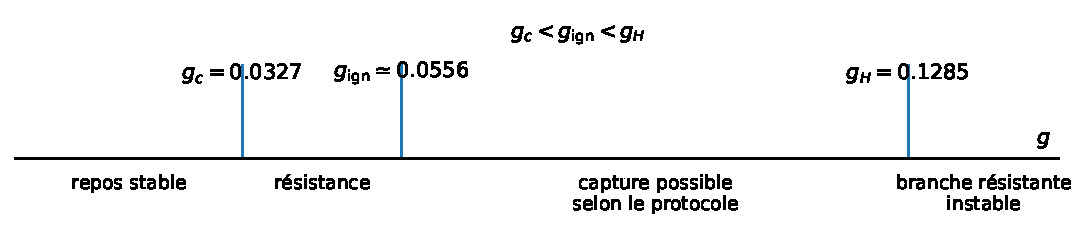
\includegraphics[width=0.96\textwidth]{fig/scientifiques/figure_trois_seuils.pdf}
\caption{Les trois seuils du protocole de référence sur un même axe. Le seuil transcritique $g_c$ et le seuil de perte de stabilité $g_H$ caractérisent la dynamique locale des branches, tandis que $g_{\mathrm{ign}}$ est un seuil de capture dépendant de la condition initiale et du protocole $\mathcal P$. La figure visualise donc une hiérarchie de mécanismes, et non trois bifurcations de même nature.}
\label{fig:t2-trois-seuils}
\end{figure}

\chapter{Définition et loi d'appropriation}\label{t2-definition-et-loi-dappropriation}

\section{Définition par les bassins {[}DEF{]}}
\label{t2-definition-par-les-bassins-def}

Soit \(z_0\) l'état de \(B\) avant l'interaction. On applique le
couplage d'intensité \(g\) pendant une durée \(T\), selon un protocole
\(\mathcal P\), puis on supprime ce couplage.

On note

\[
y_T
=
\Phi_{g,\mathcal P}^{T}(z_0)
\]

l'état obtenu au moment du découplage, et \(\omega_0(z)\) l'ensemble
limite de la dynamique autonome issue de \(z\).

\begin{quote}
\resultheading{Définition}{def:t2-appropriation}{} L'interaction \((g,T,\mathcal P)\) est appropriée
depuis \(z_0\) si

\[
\omega_0(y_T)=\mathcal A,
\qquad
\omega_0(z_0)=\mathcal A_0,
\qquad
\mathcal A\neq\mathcal A_0,
\]

où \(\mathcal A_0\) et \(\mathcal A\) sont des attracteurs autonomes de
\(B\).
\end{quote}

Cette définition exclut trois situations :

\begin{itemize}
\tightlist
\item
  une réponse temporaire qui disparaît après découplage ;
\item
  une copie maintenue uniquement par la présence de \(A\) ;
\item
  une transmission directe de la mémoire interne de \(A\).
\end{itemize}

\section{Durée minimale d'exposition}
\label{t2-duree-minimale-dexposition}

Pour une intensité \(g\), une condition initiale \(z_0\) et un protocole
\(\mathcal P\), on définit

\[
T^\ast(g;z_0,\mathcal P)
=
\inf
\left\{
T>0 :
(g,T,\mathcal P)
\text{ est appropriée depuis }z_0
\right\}.
\]

Lorsque cet ensemble est vide,

\[
T^\ast=+\infty.
\]

La notation abrégée

\[
T^\ast(g)
\]

suppose donc que la condition initiale et le protocole sont fixés.

\section{Linéarisation le long de la trace}\label{t2-linearisation-le-long-de-la-trace}

Près du repos, on linéarise la dynamique de \((x,v)\) le long de la
trajectoire temporelle de la trace :

\[
\dot z=A(t)z,
\qquad
z=
\begin{pmatrix}
x\\ v
\end{pmatrix},
\]

\[
A(t)
=
\begin{pmatrix}
0 & 1\\
\zeta-m(\sqrt2|\theta(t)|)
&
-\Gamma(\sqrt2|\theta(t)|)
\end{pmatrix}.
\]

Pendant l'exposition, \(\theta(t)\) augmente sous l'effet du terme
\(gw\). Après le découplage, elle décroît.

Lorsque

\[
m(\sqrt2|\theta(t)|)<\zeta,
\]

le coefficient linéaire de \(x\) devient positif. La petite perturbation
initiale peut alors croître.

Le calcul prédit une appropriation lorsque la trajectoire linéarisée
atteint le voisinage de l'équilibre-selle autonome positif

\[
x_u=0{,}0717
\]

avant que la décroissance de la trace ne referme la fenêtre
d'instabilité.

Ce prédicteur n'utilise pas de paramètre ajusté aux simulations.

\begin{longtable}[]{@{}rrr@{}}
\toprule\noalign{}
\(g\) & \(T^\ast\) prédit & \(T^\ast\) mesuré \\
\midrule\noalign{}
\endhead
\bottomrule\noalign{}
\endlastfoot
0,05 & aucune durée dans le régime étudié & aucune \\
0,08 & 31,6 & 31,7 \\
0,10 & 24,8 & 24,8 \\
0,15 & 17,8 & 17,9 \\
0,20 & 14,9 & 15,0 \\
0,30 & 12,2 & 12,3 \\
\end{longtable}

\begin{figure}[H]
\centering
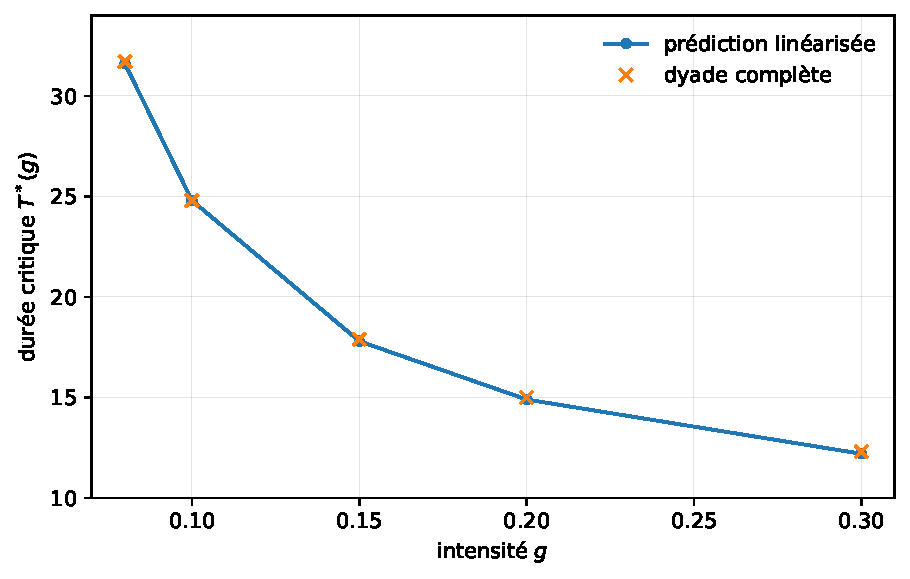
\includegraphics[width=0.90\textwidth]{fig/scientifiques/figure_duree_appropriation.pdf}
\caption{Durée critique d'appropriation pour le protocole de référence. Les points issus de la dyade complète restent au voisinage de la prédiction linéarisée, sans ajustement sur les simulations. Les valeurs numériques et le protocole de mesure sont détaillés à l'Annexe~\ref{annexe-branche-resistante-appropriation}.}
\label{fig:t2-duree-appropriation}
\end{figure}

L'écart reste inférieur à \(0{,}5\,\%\) pour les valeurs testées.

Dans la zone de résistance, prolonger l'exposition ne conduit pas à l'appropriation selon le protocole de référence. Pendant le contact, la trajectoire est capturée par la branche résistante ; après le découplage, elle revient au repos autonome.

L'analyse des trois seuils, la définition de l'appropriation par les bassins et la construction du prédicteur \(T^\ast\) sont détaillées à l'Annexe~\ref{annexe-branche-resistante-appropriation}.

\chapter{Couplage mutuel : alliance et compétition}\label{t2-couplage-mutuel-alliance-et-competition}

L'influence unidirectionnelle suffit pour définir la résistance et l'appropriation. Un couplage bidirectionnel fait apparaître deux réductions supplémentaires.

Ces réductions sont exactes sous trois conditions :

\begin{itemize}
\tightlist
\item
  les deux systèmes ont les mêmes paramètres ;
\item
  les couplages sont symétriques ;
\item
  la trajectoire reste dans le sous-espace aligné ou antipodal considéré.
\end{itemize}

\section{États alignés}\label{t2-etats-alignes}

Si

\[
h_B=h_A,
\]

alors les écritures interne et extérieure s'ajoutent :

\[
\dot\tau
=
(\alpha+g)\sigma(h)-\beta\tau.
\]

Le couplage se ramène à la transformation

\[
\alpha_{\mathrm{eff}}=\alpha+g.
\]

Pour \(g=0{,}2\), la frontière d'existence des puits actifs passe de

\[
\zeta_{\min}=0{,}3986
\]

à

\[
\zeta_{\min}=0{,}3772.
\]

Le puits commun prédit vaut \(3{,}3116\), contre \(3{,}312\) mesuré.

Le couplage aligné stabilise donc les états actifs communs dans ce
sous-espace.

\section{États antipodaux}\label{t2-etats-antipodaux}

Si

\[
h_B=-h_A,
\]

alors

\[
\sigma(h_B)=-\sigma(h_A)
\]

et

\[
\dot\tau
=
(\alpha-g)\sigma(h)-\beta\tau.
\]

Le couplage se ramène à

\[
\alpha_{\mathrm{eff}}=\alpha-g.
\]

La branche antipodale disparaît lorsque

\[
\zeta_{\min}\!\left(\frac{\alpha-g}{\beta}\right)=\zeta.
\]

Pour les paramètres de référence,

\[
g_{\mathrm{comp}}=0{,}3757.
\]

Sous ce seuil, les deux états opposés coexistent avec des puits moins profonds. Au-dessus, la configuration antipodale n'est plus disponible. Une symétrie exacte peut conduire les deux systèmes au repos. Dans les simulations, une petite asymétrie conduit généralement à leur capture dans le même puits.

Ces résultats ne couvrent pas les couplages asymétriques ni les systèmes ayant des paramètres différents.


\part{Quand l’interface devient dynamique}
\chapter{R1 : perméabilité dynamique}\label{t2-r1-permeabilite-dynamique}

Le modèle continu R0 écrit immédiatement l'influence dans la trace. R1
ajoute une variable \(q\in[0,1]\) qui représente la part effectivement
transmise.

\section{Équation de perméabilité}\label{t2-equation-de-permeabilite}

On pose

\[
\dot q
=
\rho(1-q)
-
\eta qgw.
\]

Le premier terme rouvre progressivement l'interface. Le second réduit sa
perméabilité lorsque le trafic est soutenu.

L'écriture dans la trace devient

\[
qg\,\sigma(h_A).
\]

À couplage constant,

\[
q_\infty
=
\frac{\rho}{\rho+\eta gw}
\]

et l'intensité transmise à long terme est

\[
\boxed{
g_{\mathrm{eff}}(g)
=
q_\infty g
=
\frac{\rho g}{\rho+\eta gw}
}.
\]

Elle satisfait

\[
\lim_{g\to\infty}g_{\mathrm{eff}}(g)
=
\frac{\rho}{\eta w}.
\]

\section{Transport des seuils}\label{t2-transport-des-seuils}

Soit \(g_\star^0\) un seuil du modèle continu R0. Le seuil
quasi-statique de R1 vérifie

\[
g_{\mathrm{eff}}(g_\star^{R1})=g_\star^0.
\]

On obtient

\[
\boxed{
g_\star^{R1}
=
\frac{\rho g_\star^0}
{\rho-\eta w g_\star^0}
}
\]

si

\[
\rho>\eta w g_\star^0.
\]

Dans le cas contraire, le seuil est inaccessible : la saturation de
\(g_{\mathrm{eff}}\) reste sous \(g_\star^0\).

Pour

\[
\rho=0{,}05,
\qquad
\eta=1,
\]

la formule donne

\[
g_c^{R1}=0{,}0913.
\]

Le seuil observé dynamiquement est \(0{,}0863\). La différence vient de
la condition initiale \(q(0)=1\) : le système bénéficie d'une fenêtre de
forte ouverture avant que l'interface ne se ferme.

\section{Protection de la résistance}\label{t2-protection-de-la-resistance}

Avec les mêmes paramètres,

\[
\frac{\rho}{\eta w}=0{,}0510<g_H^0.
\]

Le couplage effectif soutenu ne peut donc pas atteindre le seuil de Hopf
du modèle continu. R1 rend cette rupture inaccessible par une simple
augmentation de \(g\).

Cette protection est structurelle pour la loi de perméabilité choisie.
Elle ne prouve pas que toute interface dynamique protège la branche
résistante.

\section{Effet sur la durée d'exposition}\label{t2-effet-sur-la-duree-dexposition}

R1 allonge la durée nécessaire à l'appropriation :

\begin{longtable}[]{@{}rrr@{}}
\toprule\noalign{}
\(g\) & \(T^\ast\) sous R0 & \(T^\ast\) sous R1 \\
\midrule\noalign{}
\endhead
\bottomrule\noalign{}
\endlastfoot
0,10 & 24,8 & 88,9 \\
0,20 & 15,0 & 32,1 \\
0,30 & 12,3 & 26,2 \\
\end{longtable}

La loi R1 minimale ne produit pas d'hystérésis propre en régime stationnaire : pour chaque valeur fixée de \(g\), la dynamique de \(q\) possède un unique équilibre \(q_\infty(g)\), globalement stable.

Une hystérésis demanderait une loi supplémentaire, par exemple des seuils distincts ou plusieurs branches d'équilibre.

\chapter{R2 : écriture aux Kairos}\label{t2-r2-ecriture-aux-kairos}

R2 ne réduit pas directement l'amplitude. Il modifie le moment où
l'influence est écrite dans la trace.

\section{Accumulation à l'interface}\label{t2-accumulation-a-linterface}

L'influence s'accumule dans une variable \(\chi\) :

\[
\dot\chi
=
g\sigma(h_A)
-
\lambda_\chi\chi.
\]

Elle contribue à la pression événementielle :

\[
\dot p
=
\cdots
+
\kappa_\chi\|\chi\|.
\]

Au Kairos,

\[
\tau^+
=
\tau^-
+
\kappa_Q\chi^-,
\]

\[
\chi^+
=
(1-r_\chi)\chi^-,
\]

\[
p^+
=
r_Pp^-.
\]

Les paramètres de référence sont

\[
\lambda_\chi=0{,}2,
\qquad
\kappa_Q=0{,}6,
\qquad
r_\chi=0{,}8,
\qquad
\kappa_\chi=2{,}5.
\]

Cette version réalise une \textbf{écriture événementielle}. Elle ne
réalise pas encore une validation conditionnelle, car le quantum est
écrit quelle que soit son orientation.

\section{Validation et appropriation sont distinctes}\label{t2-validation-et-appropriation-sont-distinctes}

À \(g=0{,}10\), le protocole produit \(271\) Kairos et une trace
maximale supérieure au seuil d'instabilité, sans changement de bassin
autonome.

Le nombre d'événements ne mesure donc pas l'appropriation. Les
événements transportent la charge, mais l'issue dépend encore de la
trajectoire dans l'espace des états et de sa position par rapport aux
séparatrices.

\chapter{Application de retour du cycle événementiel}\label{t2-application-de-retour-du-cycle-evenementiel}

\section{Cycle au repos}\label{t2-cycle-au-repos}

Au repos exact,

\[
x=0,
\qquad
v=0,
\]

la dynamique de \((\chi,p)\) est autonome. Pour les paramètres étudiés et \(g>g_K\), la résolution numérique met en évidence un cycle attractif d'événements de période \(\Delta(g).\)

Entre deux Kairos, \(\chi\) suit une loi exponentielle. La condition
\(p=\Theta\) qui définit le prochain événement conduit à une équation
transcendante pour \(\Delta\).

La carte est donc explicite une fois \(\Delta\) connu, mais \(\Delta\)
doit être calculé numériquement.

\section{Carte de la trace}\label{t2-carte-de-la-trace}

Si \(\chi_\ast^-\) désigne la charge immédiatement avant un événement sur le cycle, la composante scalaire de la trace vérifie

\[
\theta_{n+1}^+
=
e^{-\beta\Delta}\theta_n^+
+
\kappa_Q\chi_\ast^-.
\]

Son point fixe est

\[
\boxed{
\theta_\infty^+
=
\frac{\kappa_Q\chi_\ast^-}
{1-e^{-\beta\Delta}}
}.
\]

La moyenne temporelle de la trace sur un cycle vaut

\[
\boxed{
\bar\theta
=
\frac{\kappa_Q\chi_\ast^-}
{\beta\Delta}
}.
\]

Cette relation donne une charge continue équivalente :

\[
\text{charge moyenne}
=
\frac{\text{quantum par événement}}
{\text{période des événements}\times\text{taux d'oubli}}.
\]

Les valeurs prédites et mesurées concordent à environ \(10^{-4}\) sur
les quatre intensités testées.

\section{Stabilité du repos}\label{t2-stabilite-du-repos}

Dans la réduction R2 considérée, la dynamique linéaire de \((x,v)\) sur le cycle est périodique. Sa stabilité est déterminée par la matrice de monodromie, c'est-à-dire par l'évolution linéaire sur une période complète.

Le cycle réduit perd sa stabilité lorsque son multiplicateur dominant traverse le cercle unité \citep{goebel2012hybrid, lakshmikantham1989impulsive}.

Le calcul donne

\[
g_F=0{,}0763.
\]

Le critère quasi-statique

\[
\bar\theta=\theta_{\mathrm{ign}}
\]

donne

\[
g_F^{qs}=0{,}0760.
\]

L'écart est de \(0{,}4\,\%\). Le cycle événementiel est suffisamment
rapide devant l'évolution de la trace pour que le modèle continu moyenné
reste une bonne approximation locale.

\chapter{Les seuils de R2}\label{t2-les-seuils-de-r2}

Quatre phénomènes doivent être séparés.

\begin{longtable}[]{@{}
  >{\raggedright\arraybackslash}p{(\columnwidth - 4\tabcolsep) * \real{0.3000}}
  >{\raggedleft\arraybackslash}p{(\columnwidth - 4\tabcolsep) * \real{0.4000}}
  >{\raggedright\arraybackslash}p{(\columnwidth - 4\tabcolsep) * \real{0.3000}}@{}}
\toprule\noalign{}
\begin{minipage}[b]{\linewidth}\raggedright
Objet
\end{minipage} & \begin{minipage}[b]{\linewidth}\raggedleft
Valeur de référence
\end{minipage} & \begin{minipage}[b]{\linewidth}\raggedright
Signification
\end{minipage} \\
\midrule\noalign{}
\endhead
\bottomrule\noalign{}
\endlastfoot
\(g_K\) & 0,03608 & apparition d'une activité événementielle soutenue \\
\(g_F\) & 0,0763 & perte de stabilité locale du cycle R2 réduit \\
\(g_{\mathrm{app}}^{R2}(x_0;\mathcal P)\) & 0,1632 & appropriation pour
la perturbation initiale et le protocole de référence \\
\(g_H^{R2}\) & \(>0{,}30\) & aucune perte de stabilité de la résistance pulsée observée jusqu'à cette borne \\ & non observée jusqu'à 0,30 & seuil éventuel non identifié \\
\end{longtable}

Le seuil \(g_K\) possède la formule

\[
g_K
=
\frac{\Theta\kappa_3\lambda_\chi}
{\kappa_\chi\sqrt2\,w}.
\]

La valeur

\[
g_{\mathrm{app}}^{R2}=0{,}1632
\]

n'est pas un analogue de \(g_c\). Elle dépend d'une condition initiale,
d'un protocole et de la cadence endogène des événements.

Enfin, les simulations ne montrent aucune perte de stabilité de la
résistance pulsée jusqu'à \(g=0{,}30\). On écrit donc

\[
g_H^{R2}>0{,}30
\]

au sens d'une borne numérique. Cette écriture ne suppose ni qu'un seuil existe au-delà, ni qu'il s'agisse nécessairement d'une bifurcation de Hopf.

Les calculs de R1 et R2, l'application de retour et le statut distinct des seuils \(g_K\), \(g_F\), \(g_{\mathrm{app}}^{R2}\) et \(g_H^{R2}\) sont détaillés à l'Annexe~\ref{annexe-interfaces-r1-r2}.

\chapter{Deux expositions : la phase de réception}\label{t2-deux-expositions-la-phase-de-reception}

\section{Protocole}\label{t2-protocole}

On applique deux expositions sous-critiques de même intensité et de même durée. Elles sont séparées par un délai \(D\).

Pour

\[
g=0{,}18,
\qquad
T_{\mathrm{sub}}=41{,}9,
\]

le balayage de \(D\) fait apparaître des bandes d'appropriation séparées
par des zones d'échec.

La période des bandes est voisine de

\[
14,
\]

à comparer à la période de la spirale libre autour du repos,

\[
\frac{2\pi}{\omega}=14{,}63,
\]

avec

\[
\omega^2=(1-\zeta)-\frac{\gamma_0^2}{4}.
\]

\section{Trois régimes}\label{t2-trois-regimes}

\subsection{Mémoire de charge}\label{t2-memoire-de-charge}

Pour

\[
D\lesssim10,
\]

la trace, la charge d'interface et la pression n'ont pas encore disparu.
Leur amplitude domine l'effet de phase.

\subsection{Mémoire de phase}\label{t2-memoire-de-phase}

Pour

\[
10\lesssim D\lesssim48,
\]

la charge résiduelle est faible, mais l'état conserve une phase dans sa
relaxation oscillante.

La seconde exposition ne rend le repos instable qu'après un temps de
charge

\[
t_c=4{,}74,
\]

mesuré indépendamment sur l'application de retour. La quantité
pertinente est donc l'état libre extrapolé au temps

\[
D+t_c.
\]

Le prédicteur est

\[
\boxed{
x_{\mathrm{lib}}(D+t_c)>0
}.
\]

Il classe correctement \(18\) cellules sur \(20\) dans le régime de
phase, sans ajustement effectué sur le scan des délais.

Les deux erreurs se trouvent aux bords des bandes.

\subsection{Extinction de l'effet}\label{t2-extinction-de-leffet}

Pour

\[
D\gtrsim50,
\]

l'amplitude résiduelle devient trop faible. Le signe seul ne suffit
plus. La capture dépend alors de l'amplitude et de la structure fine des
bassins.

\section{Pourquoi la période vaut \texorpdfstring{\(2\pi/\omega\)}{2 pi / omega}}\label{t2-pourquoi-la-periode-vaut-2piomega}

Dans une instabilité parfaitement symétrique, les deux signes de \(x\)
pourraient conduire vers deux puits opposés. On attendrait alors une
répétition tous les \(\pi/\omega\).

Ce n'est pas ce qui se produit ici.

Dans le protocole étudié :

\begin{itemize}
\tightlist
\item
  les trajectoires qui s'approprient atteignent le puits positif, autour
  de \(+2{,}30\) ;
\item
  les trajectoires arrivant du côté négatif sont capturées par la
  résistance pulsée et reviennent vers le repos.
\end{itemize}

Les deux demi-périodes ne sont donc pas équivalentes. La branche
résistante supprime une alternance sur deux, ce qui explique la période
complète

\[
2\pi/\omega.
\]

Près de l'extinction, une forme plus générale redevient nécessaire :

\[
A(D)\cos(\omega D+\varphi_0)
>
A_{\mathrm{crit}}.
\]

Dans le régime de phase, \(A_{\mathrm{crit}}\) est proche de zéro et le critère se réduit au signe. Près de \(D\simeq50\), l'amplitude redevient déterminante.

\chapter{La dose totale ne détermine pas l'issue}\label{t2-la-dose-totale-ne-determine-pas-lissue}

On définit la charge nette écrite pendant une exposition par

\[
Q_{\mathrm{net}}
=
\sum_n
\kappa_Q\chi_n^-.
\]

Deux délais donnent :

\[
Q_{\mathrm{net}}(D=14)=8{,}255,
\]

avec appropriation, et

\[
Q_{\mathrm{net}}(D=26)=8{,}322,
\]

sans appropriation.

La deuxième trajectoire reçoit une charge légèrement plus grande, mais revient au repos par la branche résistante.

\begin{quote}
\textbf{Résultat \texttt{{[}NUM{]}}.} Dans ce protocole, la quantité
totale livrée ne suffit pas à expliquer l'issue. La phase à laquelle
cette charge rencontre la dynamique interne est déterminante.
\end{quote}

Ce résultat ne signifie pas que la dose est sans effet. Il montre
qu'elle n'est pas une statistique suffisante du protocole.

\part{Ce qui reste d’une interaction}

\chapter{Amorçage par une variable lente de l'interface}\label{t2-amorcage-par-une-variable-lente-de-linterface}

R2 minimal ne conserve rien lorsque \(\tau\), \(\chi\), \(p\), \(x\) et \(v\) sont revenus à leur état de base. Pour qu'une exposition non appropriée modifie une interaction ultérieure, une variable doit persister après cet oubli.

\section{Mémoire scalaire}\label{t2-memoire-scalaire}

On introduit

\[
\dot s
=
\varepsilon_s(\chi-s),
\qquad
\varepsilon_s=0{,}005.
\]

La taille des quanta devient

\[
\kappa_Q(s)
=
\kappa_Q(1+c_ss),
\qquad
c_s=8.
\]

Après une première exposition sous-critique et un délai de \(300\), les variables transitoires sont revenues à des valeurs négligeables, mais

\[
s=0{,}0095.
\]

Le gain initial des quanta est alors supérieur de \(7{,}6\,\%\) à sa
valeur de base.

\section{Effet sur une seconde exposition}\label{t2-effet-sur-une-seconde-exposition}

Pour les durées

\[
T_2=40,\ldots,155,
\]

on observe :

\begin{longtable}[]{@{}
  >{\raggedright\arraybackslash}p{(\columnwidth - 4\tabcolsep) * \real{0.2727}}
  >{\raggedleft\arraybackslash}p{(\columnwidth - 4\tabcolsep) * \real{0.3636}}
  >{\raggedleft\arraybackslash}p{(\columnwidth - 4\tabcolsep) * \real{0.3636}}@{}}
\toprule\noalign{}
\begin{minipage}[b]{\linewidth}\raggedright
État initial de l'interface
\end{minipage} & \begin{minipage}[b]{\linewidth}\raggedleft
Cellules appropriées
\end{minipage} & \begin{minipage}[b]{\linewidth}\raggedleft
Première durée appropriante
\end{minipage} \\
\midrule\noalign{}
\endhead
\bottomrule\noalign{}
\endlastfoot
sans amorçage & 17/24 & environ 75 \\
amorçage scalaire complet & 24/24 & au plus 40 \\
\end{longtable}

La première exposition ne modifie pas immédiatement le bassin autonome,
mais elle réduit durablement la durée nécessaire à une appropriation
ultérieure.

\begin{quote}
\resultheading{Définition}{def:t2-amorcage-interface}{} Une exposition produit un \textbf{amorçage d'interface} si, après extinction des variables transitoires et sans changement immédiat de bassin autonome, elle modifie la réponse à une exposition ultérieure.
\end{quote}

\section{Tête d'avance et boucle dynamique}\label{t2-tete-davance-et-boucle-dynamique}

Un contrôle remplace la boucle dynamique par un gain constant égal au
gain initial produit par \(s\).

Les résultats sont :

\begin{longtable}[]{@{}lrr@{}}
\toprule\noalign{}
Modèle & Cellules appropriées & Première durée appropriante \\
\midrule\noalign{}
\endhead
\bottomrule\noalign{}
\endlastfoot
sans amorçage & 17 & 75 \\
gain constant \(+7{,}6\,\%\) & 23 & 45 \\
boucle complète & 24 & 40 \\
\end{longtable}

L'essentiel de l'amorçage vient donc de la tête d'avance présente au
début de la seconde exposition. La rétroaction, dans laquelle des quanta
plus grands alimentent ensuite \(s\), ajoute un effet secondaire.

La formulation correcte est :

\[
\text{amorçage}
=
\text{gain initial persistant}
+
\text{amplification dynamique secondaire}.
\]

\section{Temps fini et contact soutenu}\label{t2-temps-fini-et-contact-soutenu}

Le résidu de \(s\) modifie fortement la durée critique d'une rencontre
finie. Il modifie très peu le seuil d'appropriation sous contact soutenu
:

\[
\Delta g_{\mathrm{app}}\simeq-0{,}0014.
\]

Sur un temps suffisamment long, \(s\) se recharge dans les deux
conditions. La mémoire de l'interface change donc surtout ce qui est
accessible pendant la durée d'une interaction, non l'ensemble des
comportements possibles sous contact permanent.

\chapter{Limite de la mémoire scalaire}\label{t2-limite-de-la-memoire-scalaire}

La variable \(s\) précédente dépend de l'intensité de \(\chi\), pas de
sa direction. Elle mémorise qu'une exposition a eu lieu, sans distinguer
ce qui a été reçu.

Le contrôle directionnel confirme cette limite.

Après une amorce et un oubli, on applique une seconde exposition :

\begin{itemize}
\tightlist
\item
  dans la même direction ;
\item
  dans une direction orthogonale ;
\item
  dans la direction opposée.
\end{itemize}

La perturbation initiale de l'état est rétablie au début de la seconde exposition afin que sa décroissance pendant le délai ne masque pas l'effet de l'interface. Cette remise à la graine fait partie du protocole de contrôle.

Pour la mémoire scalaire :

\begin{longtable}[]{@{}lr@{}}
\toprule\noalign{}
Seconde exposition & Cellules appropriées \\
\midrule\noalign{}
\endhead
\bottomrule\noalign{}
\endlastfoot
même direction & 5/12 \\
orthogonale & 5/12 \\
opposée & 5/12 \\
base sans amorce & 2/12 \\
\end{longtable}

L'amorçage est global. Il facilite de la même manière les trois
directions.

\chapter{Mémoire directionnelle et compatibilité}\label{t2-memoire-directionnelle-et-compatibilite}

\section{Variable vectorielle}\label{t2-variable-vectorielle}

On remplace \(s\) par une variable vectorielle :

\[
\dot{\mathbf s}
=
\varepsilon_s(\boldsymbol\chi-\mathbf s).
\]

Elle conserve une direction moyenne des expositions récentes.

Au Kairos, la trace reçoit

\[
\boxed{
\tau^+
=
\tau^-
+
\max\!\left(
1+c_s\langle\mathbf s,\widehat{\boldsymbol\chi}\rangle,
0
\right)
\kappa_Q\boldsymbol\chi^-
}
\]

avec

\[
\widehat{\boldsymbol\chi}
=
\frac{\boldsymbol\chi}
{\|\boldsymbol\chi\|}
\]

lorsque \(\boldsymbol\chi\neq0\).

Le facteur de compatibilité dépend du produit scalaire entre la mémoire
lente de l'interface et l'exposition présente.

\section{Trois cas}\label{t2-trois-cas}

Si l'exposition présente est alignée avec \(\mathbf s\),

\[
\langle\mathbf s,\widehat{\boldsymbol\chi}\rangle>0,
\]

et le quantum est augmenté.

Si elle est orthogonale,

\[
\langle\mathbf s,\widehat{\boldsymbol\chi}\rangle=0,
\]

et le quantum conserve sa taille de base.

Si elle est opposée,

\[
\langle\mathbf s,\widehat{\boldsymbol\chi}\rangle<0,
\]

et le quantum est réduit.

La borne inférieure à zéro empêche une anti-écriture dans laquelle un
quantum inversé effacerait artificiellement la trace.

\section{Résultats}\label{t2-resultats}

\begin{longtable}[]{@{}
  >{\raggedright\arraybackslash}p{(\columnwidth - 8\tabcolsep) * \real{0.1579}}
  >{\raggedleft\arraybackslash}p{(\columnwidth - 8\tabcolsep) * \real{0.2105}}
  >{\raggedleft\arraybackslash}p{(\columnwidth - 8\tabcolsep) * \real{0.2105}}
  >{\raggedleft\arraybackslash}p{(\columnwidth - 8\tabcolsep) * \real{0.2105}}
  >{\raggedleft\arraybackslash}p{(\columnwidth - 8\tabcolsep) * \real{0.2105}}@{}}
\toprule\noalign{}
\begin{minipage}[b]{\linewidth}\raggedright
Mémoire de l'interface
\end{minipage} & \begin{minipage}[b]{\linewidth}\raggedleft
Même direction
\end{minipage} & \begin{minipage}[b]{\linewidth}\raggedleft
Orthogonale
\end{minipage} & \begin{minipage}[b]{\linewidth}\raggedleft
Opposée
\end{minipage} & \begin{minipage}[b]{\linewidth}\raggedleft
Base
\end{minipage} \\
\midrule\noalign{}
\endhead
\bottomrule\noalign{}
\endlastfoot
scalaire & 5/12 & 5/12 & 5/12 & 2/12 \\
vectorielle & 5/12 & 2/12 & 1/12 & 2/12 \\
\end{longtable}

La mémoire vectorielle produit donc :

\begin{itemize}
\tightlist
\item
  une facilitation pour une exposition de même direction ;
\item
  une neutralité mesurée pour une exposition orthogonale ;
\item
  une inhibition pour une exposition opposée.
\end{itemize}

Ces trois effets proviennent d'une seule règle. Ils ne sont pas
implémentés par trois mécanismes séparés.

Nous parlerons ici d'\textbf{inhibition directionnelle} plutôt que
d'habituation au sens strict. Une habituation demanderait de montrer
qu'une répétition du même signal réduit progressivement la réponse, ce
que ce protocole ne montre pas.

\section{Statut de l'intégration conditionnelle}\label{t2-statut-de-lintegration-conditionnelle}

R2 minimal écrivait tout quantum présent au Kairos. La règle vectorielle
introduit pour la première fois une condition calculée à partir de
l'histoire de l'interface.

Elle ne décide pas seulement si une écriture a lieu. Elle module le
canal futur selon la relation entre ce qui a été reçu et ce qui arrive
maintenant.

\begin{quote}
\textbf{Résultat \texttt{{[}NUM{]}}.} Deux interfaces ayant reçu des
histoires différentes répondent différemment à la même intensité future,
alors que leurs variables rapides ont été ramenées à la même condition
de départ.
\end{quote}

Ce résultat établit une mémoire spécifique au contenu directionnel reçu.
Il ne permet pas encore de distinguer deux partenaires qui produiraient
exactement la même projection.

\chapter{Appropriation, amorçage et mémoire spécifique}\label{t2-appropriation-amorcage-et-memoire-specifique}

Trois transformations doivent maintenant être distinguées.

\section{Appropriation}\label{t2-appropriation-1}

Une appropriation change le bassin autonome atteint après la fin de
l'interaction :

\[
\mathcal A_0
\longrightarrow
\mathcal A_1.
\]

\section{Amorçage}\label{t2-amorcage}

Un amorçage laisse le système dans le même bassin immédiat, mais modifie l'accessibilité d'une transition future, par exemple sa durée minimale d'exposition :

\[
T_2^\ast
\neq
T_1^\ast.
\]

\section{Mémoire spécifique}\label{t2-memoire-specifique}

Une mémoire spécifique modifie sélectivement la réponse future selon la relation entre l'histoire de l'interface et le signal présent :

\[
T^\ast(\varphi)
\]

dépend de l'angle relatif \(\varphi\).

L'appropriation porte sur les attracteurs. L'amorçage porte sur leur accessibilité. La mémoire directionnelle rend cette accessibilité dépendante de la relation entre le contenu reçu et l'exposition présente.

\chapter{Ce que le Tome II établit}\label{t2-ce-que-le-tome-ii-etablit}

La dyade minimale fournit les résultats suivants.

\begin{enumerate}
\def\labelenumi{\arabic{enumi}.}
\tightlist
\item
  Une influence conforme agit par la trace et ne déplace pas directement un repos exact.
\item
  Une charge suffisante peut rendre le repos instable.
\item
  Entre l'inertie et l'appropriation existe une branche résistante antiparallèle.
\item
    Cette branche naît par une bifurcation transcritique et connaît une rupture de stabilité de type Hopf dans le modèle continu.
\item
  Le seuil de capture d'une condition initiale n'est pas une bifurcation ; il dépend du protocole.
\item
  L'appropriation se définit par un changement de bassin autonome après découplage.
\item
  La perméabilité dynamique R1 étudiée protège en saturant l'intensité transmise.
\item
  Une écriture aux Kairos crée un cycle événementiel et sépare activité événementielle, stabilité locale et appropriation.
\item
  Deux expositions identiques peuvent produire des issues différentes selon la phase de réception.
\item
  Une variable lente de l'interface peut conserver l'effet d'une exposition non appropriée.
\item
  Une mémoire scalaire produit une sensibilisation générale.
\item
  Une mémoire vectorielle produit une réponse sélective à la direction du contenu reçu.
\end{enumerate}

Les protocoles numériques soutenant les valeurs \textnormal{[PROP-NUM]}, les bandes de phase ainsi que les contrôles d'amorçage et de mémoire directionnelle sont rassemblés à l'Annexe~\ref{annexe-methodes-validations-numeriques}.

Ces résultats ne montrent pas encore :

\begin{itemize}
\tightlist
\item
  que les mêmes mécanismes persistent dans une dyade de réseaux hors de
  la variété homogène ;
\item
  qu'un seuil de perte de stabilité de la résistance pulsée existe
  au-delà de \(g=0{,}30\) ;
\item
  que le prédicteur de bandes est exact aux bords des fenêtres ;
\item
  que la mémoire directionnelle distingue les partenaires et pas
  seulement les projections ;
\item
  que plusieurs amorçages se composent d'une manière irréductible à une
  somme pondérée ;
\item
  que l'ordre des expositions produit une trajectoire individuelle qui
  ne se réduit pas à la récence.
\end{itemize}

\chapter{Passage vers le Tome III}\label{t2-passage-vers-le-tome-iii}

Le Tome III devra étudier la composition des transformations
précédentes.

Soient deux histoires \(\mathcal H_1\) et \(\mathcal H_2\). On associe à
chaque histoire une fonction de réponse

\[
\mathcal R_{\mathcal H}(u)
=
\left(
T^\ast_{\mathcal H}(u),
g_{\mathrm{app},\mathcal H}(u),
\mathcal A_{\infty,\mathcal H}(u)
\right).
\]

Deux histoires sont séparables par une même famille de sondes si elles conduisent à des réponses différentes.

La première question est celle de l'ordre :

\[
\mathcal R_{\mathcal H_1\cdot\mathcal H_2}
\stackrel{?}{=}
\mathcal R_{\mathcal H_2\cdot\mathcal H_1}.
\]

Avec la dynamique linéaire actuelle de \(\mathbf s\), une différence
peut provenir simplement de la récence. Le problème sera donc de
distinguer :

\begin{itemize}
\tightlist
\item
  une pondération temporelle ordinaire ;
\item
  une composition non commutative des expériences ;
\item
  une restructuration persistante de la fonction de réponse.
\end{itemize}

Le point de départ est maintenant défini : une trajectoire individuelle
devra être décrite non seulement par les attracteurs déjà atteints, mais
par la manière dont les interactions passées ont modifié l'accessibilité
des attracteurs futurs.

\tome{III}{La persistance des histoires}

\hspace{0pt}
\vfill
\planche{10.6cm}{fig/planche_III_question.pdf}
{Tome III — La question qui sépare}
{Deux réalisations superposées. Leurs chemins diffèrent partout, et cela ne
change rien~: elles rejoignent les mêmes états et partagent exactement la même
frontière. Une différence infime, invisible ailleurs, les envoie vers des
issues opposées~— sur moins d'un degré d'interrogation.}
\vfill
\hspace{0pt}
\newpage
\part{Des histoires à l'observation}
\chapter{Des trajectoires aux histoires}\label{t3-des-trajectoires-aux-histoires}

Le Tome II s'est achevé sur une question de composition.

À chaque histoire $\mathcal H$ était associée une fonction de réponse
\[
\mathcal R_{\mathcal H}(u)
=
\left(
T^\ast_{\mathcal H}(u),
g_{\mathrm{app},\mathcal H}(u),
\mathcal A_{\infty,\mathcal H}(u)
\right),
\]
et la possibilité d'une dépendance à l'ordre était formulée par
\[
\mathcal R_{\mathcal H_1\cdot\mathcal H_2}
\stackrel{?}{=}
\mathcal R_{\mathcal H_2\cdot\mathcal H_1}.
\]

Cette écriture indiquait déjà le problème, mais elle ne suffisait pas encore à le poser complètement.

En effet, une différence entre les deux membres peut avoir plusieurs origines. Elle peut résulter d'une simple pondération de récence, d'une non-commutativité effective des expériences, ou d'une modification plus profonde de la manière dont le système répond désormais aux interventions futures. Ces mécanismes ne peuvent être distingués à partir de la seule comparaison de deux trajectoires.

Il faut d'abord préciser ce que l'on appelle une histoire, ce qui en survit dans l'état présent, et selon quelles lectures deux histoires peuvent être considérées comme fonctionnellement distinctes.

Le Tome III prend donc pour objet non plus seulement l'évolution d'un système, mais la relation entre les transformations qu'il a traversées et l'espace de ses réponses futures.

La question directrice devient alors :
\begin{quote}
\itshape À quelles conditions deux réalisations d’un même système initial, soumises à des histoires différentes, demeurent-elles séparables par leurs réponses futures ?
\end{quote}
La séparation ne porte donc pas directement sur les passés eux-mêmes, mais sur les transformations qu’ils ont laissées dans les réalisations du système et sur les différences de réponse que des interventions ultérieures permettent encore de révéler.

Cette progression conduira successivement à :

\begin{itemize}
\tightlist
\item
  définir les histoires et leurs lectures ;
\item
  isoler leur contenu survivant ;
\item
  déterminer quand un état lent suffit à en résumer les effets ;
\item
  décrire les frontières où les réponses changent ;
\item
  distinguer les propriétés du comportement de celles de sa présentation ;
\item
  construire enfin une géométrie de la séparabilité entre histoires.
\end{itemize}

Le point de départ reste celui posé à la fin du Tome II : une trajectoire individuelle ne se caractérise pas seulement par les attracteurs déjà atteints, mais par la manière dont les interactions passées ont modifié l'accessibilité des attracteurs futurs.

Le premier pas consiste maintenant à donner un sens formel au mot
\emph{histoire}.

\section{Pourquoi la trajectoire ne suffit pas}
\label{t3-pourquoi-la-trajectoire-ne-suffit-pas}

Une trajectoire décrit l'évolution effective d'une réalisation du système. Elle ordonne les états traversés, les événements rencontrés et les transformations produites au cours du temps.

Cette description ne suffit toutefois pas à caractériser ce que le système est devenu.

Deux réalisations peuvent atteindre des états instantanés proches, voire identiques au regard des variables observées, tout en ne répondant plus de la même manière aux interventions ultérieures. Inversement, deux trajectoires très différentes peuvent conduire à des réalisations que plus aucune sonde admissible ne permet de distinguer.

La différence entre les trajectoires passées n'est donc ni une condition suffisante ni une condition nécessaire de la séparabilité future.

Le problème du Tome III ne consiste pas à comparer directement des chemins dans l'espace d'état. Il consiste à déterminer ce que ces chemins ont laissé dans les réalisations qui les ont suivis.

Soit une réalisation initiale $X_0$, soumise à une histoire $\mathcal H$. À l'issue de cette histoire, on obtient une réalisation transformée que l'on peut noter provisoirement
\[
X_{\mathcal H}.
\]

Cette notation ne suppose pas que toute l'histoire soit encodée dans un état instantané, ni qu'elle puisse être reconstruite à partir de celui-ci. Elle indique seulement que les réponses futures du système peuvent dépendre de l'histoire qu'il a traversée.

Soumise à une intervention ultérieure $u$, la réalisation
$X_{\mathcal H}$ produit une réponse
\[
\mathcal R_{\mathcal H}(u).
\]

Deux histoires $\mathcal H_1$ et $\mathcal H_2$, appliquées à deux réalisations comparables du même système initial, demeurent fonctionnellement séparables s'il existe au moins une intervention admissible $u$ telle que
\[
\mathcal R_{\mathcal H_1}(u)
\neq
\mathcal R_{\mathcal H_2}(u).
\]

La comparaison porte ainsi sur un diagramme de la forme
\[
X_0
\;\xrightarrow{\;\mathcal H_j\;}\;
X_{\mathcal H_j}
\;\xrightarrow{\;u\;}\;
\mathcal R_{\mathcal H_j}(u),
\qquad j\in\{1,2\}.
\]

L'histoire intervient donc à deux niveaux distincts.

D'une part, elle décrit une succession effective de transformations. D'autre part, elle désigne ce qui, dans cette succession, demeure encore capable de modifier les réponses futures.

Ces deux niveaux ne doivent pas être confondus. Une partie du passé peut avoir eu lieu sans demeurer fonctionnellement active. À l'inverse, une transformation brève peut laisser une modification persistante de l'accessibilité des régimes futurs.

Il faut dès lors distinguer trois objets :

\begin{itemize}
\tightlist
\item
  la trajectoire effectivement parcourue ;
\item
  l'histoire en tant que composition de transformations ;
\item
  le contenu de cette histoire qui survit dans les réponses futures.
\end{itemize}

La première étape consiste à préciser le deuxième de ces objets. Le contenu survivant ne pourra être défini qu'une fois établi ce qui compte comme une histoire, comment plusieurs épisodes s'y composent, et selon quelles lectures cette histoire est interrogée.

\section{Histoires, épisodes et composition}
\label{t3-histoires-episodes-composition}

Une histoire n'est pas introduite comme une trajectoire continue supplémentaire. Elle décrit l'ordre dans lequel une réalisation du système traverse une suite d'épisodes susceptibles de la transformer.

Soit $\mathcal E$ l'ensemble des épisodes admissibles. À chaque épisode $e\in\mathcal E$ est associée une application de transition
\[
\Phi_e:\mathfrak X\longrightarrow\mathfrak X,
\]
où $\mathfrak X$ désigne l'espace dans lequel est représentée la réalisation du système.

Une histoire finie est un mot
\[
\mathcal H=e_1e_2\cdots e_n.
\]
Elle se lit de gauche à droite dans l'ordre chronologique : le système vit d'abord $e_1$, puis $e_2$, et ainsi de suite jusqu'à $e_n$.

La transformation induite par cette histoire est
\[
\Phi_{\mathcal H}
=
\Phi_{e_n}\circ\cdots\circ\Phi_{e_1}.
\]
L'histoire vide est notée $\varepsilon$ et vérifie
\[
\Phi_{\varepsilon}
=
\operatorname{Id}_{\mathfrak X}.
\]

Cette distinction entre l'ordre d'écriture de l'histoire et l'ordre de composition des applications sera conservée dans tout le Tome III.

Si $\mathcal H_1$ et $\mathcal H_2$ sont deux histoires, leur concaténation
\[
\mathcal H_1\cdot\mathcal H_2
\]
désigne l'histoire dans laquelle le système vit d'abord $\mathcal H_1$, puis $\mathcal H_2$. Par conséquent,
\begin{equation}
\label{eq:t3-composition-histoires}
\boxed{
\Phi_{\mathcal H_1\cdot\mathcal H_2}
=
\Phi_{\mathcal H_2}\circ\Phi_{\mathcal H_1}.
}
\end{equation}

L'histoire et la transition qu'elle induit ne doivent cependant pas être identifiées.

Deux histoires différentes peuvent produire la même transformation :
\[
\mathcal H_1\neq\mathcal H_2,
\qquad
\Phi_{\mathcal H_1}
=
\Phi_{\mathcal H_2}.
\]
Dans ce cas, leur différence chronologique ne laisse aucune différence dans la réalisation finale, du moins à l'échelle décrite par $\mathfrak X$.

Réciproquement, deux transitions distinctes peuvent ne pas être distinguées par les réponses que l'on choisit d'observer :
\[
\Phi_{\mathcal H_1}
\neq
\Phi_{\mathcal H_2},
\]
sans qu'il existe nécessairement, parmi les sondes admissibles, une intervention $u$ telle que
\[
\mathcal R_{\mathcal H_1}(u)
\neq
\mathcal R_{\mathcal H_2}(u).
\]

Trois niveaux de comparaison apparaissent ainsi :

\begin{itemize}
\tightlist
\item
  la différence entre les mots historiques ;
\item
  la différence entre les transitions qu'ils induisent ;
\item
  la différence entre les réponses futures que les sondes permettent
  effectivement de révéler.
\end{itemize}

Ces niveaux ne coïncident pas en général.

La question de l'ordre formulée à la fin du Tome II doit donc être précisée. Au niveau des histoires, elle oppose
\[
\mathcal H_1\cdot\mathcal H_2
\qquad\text{et}\qquad
\mathcal H_2\cdot\mathcal H_1.
\]
Au niveau des transitions, elle devient
\[
\Phi_{\mathcal H_2}\circ\Phi_{\mathcal H_1}
\stackrel{?}{=}
\Phi_{\mathcal H_1}\circ\Phi_{\mathcal H_2}.
\]
Au niveau des réponses futures, elle s'écrit
\[
\mathcal R_{\mathcal H_1\cdot\mathcal H_2}(u)
\stackrel{?}{=}
\mathcal R_{\mathcal H_2\cdot\mathcal H_1}(u)
\]
pour les interventions admissibles $u$.

Une différence observée au dernier niveau établit que l'ordre demeure fonctionnellement détectable. Elle ne suffit toutefois pas à identifier le mécanisme qui la produit.

Dans le modèle actuel, l'épisode vécu en dernier peut peser davantage sur l'état lent simplement parce que son effet a subi moins d'atténuation. L'échange de deux épisodes modifie alors la réponse sans qu'il soit encore nécessaire d'invoquer une restructuration durable de l'organisation interne.

Il faut donc distinguer deux affirmations :

\begin{enumerate}
\item
  l'ordre des épisodes modifie la réponse future ;
\item
  l'histoire a modifié de manière persistante la façon dont le système transforme les interventions futures.
\end{enumerate}

La première porte sur une différence observable. La seconde porte sur la nature de ce qui survit à l'histoire. Elle exige davantage qu'une simple comparaison entre deux états terminaux ou entre deux valeurs instantanées de la fonction de réponse.

Le problème n'est donc plus seulement de savoir si
\[
\mathcal H_1\cdot\mathcal H_2
\quad\text{et}\quad
\mathcal H_2\cdot\mathcal H_1
\]
produisent des résultats différents. Il est de déterminer quelle part de cette différence demeure active, sous quelles interventions elle peut être révélée, et si elle peut être expliquée par le seul écoulement du temps.

La notion d'histoire étant désormais posée, il reste à préciser comment elle est interrogée. Une différence passée ne devient fonctionnellement pertinente qu'à travers les lectures capables d'en révéler les effets.

\section{Sondes, lectures et séparabilité relative}
\label{t3-sondes-lectures-separabilite}

Une différence entre deux réalisations ne devient fonctionnellement pertinente que si une intervention permet de la révéler et si une lecture permet d'en comparer les effets.

Il faut donc distinguer ce que l'on fait vivre au système de ce que l'on observe de son exécution.

\subsection{Toute sonde est une histoire}

Soit
\[
\mathfrak M=\mathcal E^\ast
\]
le monoïde des histoires finies introduit précédemment. Un protocole d'observation déclare une classe
\[
\mathfrak B\subseteq\mathfrak M
\]
d'histoires admissibles.

Une sonde n'est donc pas nécessairement une intervention instantanée. Elle peut comprendre une exposition, une attente, une regraine, une relaxation ou une composition de plusieurs de ces épisodes. Elle est elle-même une histoire.

\subsection{Ce qu'une sonde permet de lire}

Lorsqu'une réalisation $X$ est soumise à une histoire de sonde $\mathcal H$, elle produit une exécution
\[
\operatorname{Exec}_{\mathcal H}(X).
\]

Cette exécution rassemble tout ce qui s'est produit pendant la sonde : la trajectoire continue, les événements éventuels, les états avant et après chaque saut, ainsi que l'état terminal.

Une expérience ne retient cependant pas nécessairement toute cette information.

Elle peut, par exemple, observer seulement :

\begin{itemize}
\tightlist
\item
  l'attracteur finalement atteint ;
\item
  le nombre de Kairos produits ;
\item
  leur calendrier ;
\item
  ou une portion particulière de la trajectoire.
\end{itemize}

On note $\rho$ le choix de ce qui est ainsi retenu. Dans la suite, $\rho$ désignera donc une \emph{lecture}, ou de manière équivalente une résolution d'observation.

Le symbole $\rho$ ne décrit pas une variable interne du système. Il appartient au protocole utilisé pour l'interroger.

Pour une lecture fixée, la réponse observée est notée
\[
\mathcal R_X^\rho(\mathcal H).
\]

Le passage de l'exécution à la réponse peut être représenté par
\[
\operatorname{Exec}_{\mathcal H}(X)
\;\xrightarrow{\;\rho\;}\;
\mathcal R_X^\rho(\mathcal H).
\]

Une lecture terminale ne conserve que ce qui peut être déterminé à partir de l'état atteint à la fin de la sonde. Elle peut notamment indiquer le bassin terminal ou l'attracteur rejoint.

Une lecture de chemin conserve au contraire une information produite pendant l'exécution : le nombre d'événements, leur ordre, leur calendrier ou certaines caractéristiques de la trajectoire.

Deux réalisations peuvent ainsi atteindre le même attracteur tout en l'atteignant par des chemins différents. Elles seront indiscernables pour une lecture terminale qui ne conserve que l'attracteur, mais pourront être séparées par une lecture de chemin plus fine.

Inversement, deux exécutions mathématiquement différentes peuvent conduire à la même réponse lorsque la lecture choisie ne conserve pas ce qui les distingue.

La réponse dépend donc de trois éléments :
\[
\text{la réalisation interrogée},
\qquad
\text{l'histoire de sonde},
\qquad
\text{la lecture retenue}.
\]

L'écriture employée à la fin du Tome II peut maintenant être précisée.

Lorsque l'état initial $X_0$, la lecture $\rho$ et une famille de sondes paramétrées par $u$ sont laissés implicites, l'expression
\[
\mathcal R_{\mathcal H_0}(u)
\]
désigne la réponse obtenue après qu'une réalisation initiale a vécu l'histoire $\mathcal H_0$, puis a été soumise à la sonde associée à $u$.

En développant les éléments restés implicites, cette réponse s'écrit
\[
\mathcal R_{\Phi_{\mathcal H_0}(X_0)}^\rho
\bigl(\mathcal H_u\bigr).
\]
\subsection{Une équivalence déclarée}
\label{t3-equivalence-declaree}

Une fois fixées les histoires de sonde admissibles et la lecture retenue, la comparaison de deux réalisations devient précise.

Soient deux réalisations
\[
X,Y\in\mathfrak X.
\]

Elles sont dites \emph{équivalentes en réponse} relativement à la classe de sondes \(\mathfrak B\) et à la lecture \(\rho\) lorsque toute histoire admissible produit la même réponse à partir de $X$ et de $Y$ :
\begin{equation}
\label{eq:t3-equivalence-observationnelle}
\boxed{
X\sim_{\mathfrak B,\rho}Y
\quad\Longleftrightarrow\quad
\forall\mathcal H\in\mathfrak B,
\qquad
\mathcal R_X^\rho(\mathcal H)
=
\mathcal R_Y^\rho(\mathcal H).
}
\end{equation}

Cette définition ne compare donc pas directement les états internes de $X$ et de $Y$. Elle compare ce qu'ils donnent à voir lorsqu'ils sont soumis aux mêmes histoires de sonde et lus de la même manière.

À l'inverse, les deux réalisations sont séparables dans le protocole déclaré s'il existe au moins une histoire
\[
\mathcal H\in\mathfrak B
\]
telle que
\[
\mathcal R_X^\rho(\mathcal H)
\neq
\mathcal R_Y^\rho(\mathcal H).
\]

Une telle histoire sera dite \emph{séparatrice} pour $X$ et $Y$ à la lecture $\rho$.

La séparabilité possède ainsi un témoin explicite :
\[
X\not\sim_{\mathfrak B,\rho}Y
\quad\Longleftrightarrow\quad
\exists\mathcal H\in\mathfrak B
\ \text{telle que}\
\mathcal R_X^\rho(\mathcal H)
\neq
\mathcal R_Y^\rho(\mathcal H).
\]

L'absence de sonde séparatrice ne permet toutefois pas de conclure que les deux réalisations sont identiques.

Elle signifie seulement qu'elles ne peuvent pas être distinguées dans les limites du protocole considéré.

Deux réalisations peuvent ainsi être équivalentes pour une classe de sondes brèves et cesser de l'être lorsque des histoires plus longues sont autorisées. Elles peuvent également être équivalentes pour une lecture terminale ne retenant que l'attracteur atteint, mais devenir
séparables lorsqu'on observe le chemin suivi ou le calendrier des événements.

L'équivalence dépend donc conjointement de deux choix :
\[
\mathfrak B,
\qquad
\rho.
\]

Le premier détermine ce qu'il est permis de faire vivre au système. Le second détermine ce qui est retenu de ses réponses.

Ces choix n'introduisent aucune finalité dans la dynamique. Ils ne désignent ni un objectif poursuivi par le système, ni une norme à laquelle il devrait se conformer. Ils déclarent seulement les moyens dont dispose l'observation pour faire apparaître une différence.

Il n'existe donc pas, dans ce cadre, de critère absolu de séparation donné une fois pour toutes. Une différence peut être inaccessible à un protocole et détectable par un autre.

Cette relativité n'affaiblit pas la comparaison. Elle en précise la portée.

Affirmer
\[
X\sim_{\mathfrak B,\rho}Y
\]
revient à dire exactement que, pour les sondes et la lecture déclarées, $X$ et $Y$ possèdent le même profil de réponse.

Le cadre formel des histoires admissibles, du transport de l'équivalence par préfixe et du raffinement des quotients lorsque la classe de sondes ou la résolution sont enrichies est donné à l'Annexe~\ref{annexe-histoires-equivalences}.

Le jeu des différences ne consiste donc pas à supposer qu'une différence doit nécessairement être trouvée. Il consiste à rechercher une histoire capable de la manifester et à reconnaître, lorsqu'aucune histoire admissible n'y parvient, que les deux réalisations appartiennent à une même classe d'observation.

Cette équivalence permet désormais de revenir aux histoires déjà vécues.

Si deux histoires conduisent, à partir d'une même réalisation initiale, à des réalisations indiscernables, alors leur différence n'est plus accessible au protocole déclaré. Si elles conduisent à des réalisations séparables, une partie de leur différence demeure encore active.

Il reste à déterminer ce qui, dans une histoire passée, porte cette capacité de séparation.

\section{Ce qui survit d'une histoire}
\label{t3-contenu-survivant}

Deux histoires différentes ne laissent pas nécessairement deux réalisations durablement différentes.

Soit une même réalisation initiale
\[
X_0\in\mathfrak X,
\]
soumise à deux histoires $\mathcal H_1$ et $\mathcal H_2$. À l'issue de ces histoires, on obtient
\[
X_1=\Phi_{\mathcal H_1}(X_0),
\qquad
X_2=\Phi_{\mathcal H_2}(X_0).
\]

La différence entre $\mathcal H_1$ et $\mathcal H_2$ demeure accessible au protocole déclaré s'il existe une sonde admissible qui produit, à partir de $X_1$ et de $X_2$, deux réponses différentes.

À l'inverse, si
\[
\Phi_{\mathcal H_1}(X_0)
\sim_{\mathfrak B,\rho}
\Phi_{\mathcal H_2}(X_0),
\]
alors toutes les sondes admissibles produisent, selon la lecture retenue, la même réponse à partir des deux réalisations.

Les deux histoires ne sont pas devenues identiques. Elles demeurent deux mots distincts, composés d'épisodes éventuellement différents et vécus dans des ordres différents. Mais leur distinction passée ne possède plus de conséquence accessible dans les réponses futures considérées.

Lorsque la réalisation initiale et le protocole sont fixés, on pourra écrire plus simplement
\[
\mathcal H_1\equiv\mathcal H_2
\]
pour indiquer cette équivalence fonctionnelle entre histoires.

Cette relation ne classe donc pas les histoires selon ce qui s'est effectivement produit. Elle les classe selon ce que leurs effets permettent encore de distinguer.

\subsection{L'oubli comme perte de pouvoir de séparation}

L'oubli peut alors recevoir une première caractérisation fonctionnelle.

Oublier une différence entre deux histoires ne signifie pas nécessairement effacer toute trace matérielle de cette différence. Il suffit que les traces restantes ne puissent plus modifier les réponses observées dans le protocole déclaré.

Une différence peut ainsi subsister dans une variable interne sans être fonctionnellement active. Elle peut également devenir inaccessible parce que les sondes admises sont trop faibles, trop brèves ou trop peu diversifiées pour la révéler.

L'oubli est donc lui aussi relatif à
\[
(\mathfrak B,\rho).
\]

Une distinction perdue pour une lecture terminale peut subsister pour une lecture de chemin. Une distinction invisible sous des sondes courtes peut réapparaître lorsqu'une histoire plus longue est autorisée.

Il ne faut donc pas confondre :

\begin{itemize}
\tightlist
\item
  la disparition d'une variable ;
\item
  l'inactivité fonctionnelle d'une différence ;
\item
  l'impossibilité de détecter cette différence avec le protocole retenu.
\end{itemize}

La première est une propriété de la dynamique interne. La deuxième porte sur l'effet futur de ce qui demeure. La troisième dépend également des moyens d'intervention et de lecture.

\subsection{Un contenu n'est pas un récit}

On appellera \emph{contenu survivant} d'une histoire ce qui doit être préservé pour conserver son profil de réponses futures.

Cette expression ne désigne pas une copie abrégée de l'histoire.

Le contenu survivant n'a pas à indiquer quels épisodes ont été vécus, dans quel ordre ils l'ont été, ni à quel instant ils se sont produits. Il doit seulement conserver les différences encore capables d'affecter les réponses ultérieures.

Plusieurs histoires distinctes peuvent ainsi produire le même profil de réponses futures :
\[
\mathcal H_1\neq\mathcal H_2,
\qquad
\mathcal H_1\equiv\mathcal H_2.
\]

La première relation indique que les épisodes vécus, ou leur ordre, diffèrent. La seconde indique que cette différence ne modifie plus aucune réponse accessible dans le protocole déclaré.

Le contenu survivant devra précisément représenter ce qui distingue encore les histoires du point de vue de leurs réponses futures, sans avoir à conserver les différences devenues fonctionnellement inertes.

Ce qui le définit n'est pas son écriture interne, mais sa suffisance : deux réalisations portant le même contenu survivant doivent répondre de la même manière aux sondes déclarées.

L'histoire complète et son contenu survivant jouent ainsi des rôles
différents :
\[
\textit{l'histoire décrit ce qui a été vécu, le contenu survivant décrit ce qui agit encore}.
\]

Le passage de l'une à l'autre constitue une compression. Cette compression est légitime lorsqu'elle ne retire aucune information nécessaire à la détermination des réponses futures.

Le problème devient alors précis : sous quelles conditions la réponse d'une réalisation ne dépend-elle plus de l'ensemble de son histoire, mais seulement d'un état résiduel plus simple ?

Dans le régime étudié ci-après, la relaxation éteint certaines composantes rapides tandis qu'une variable lente demeure. Il faudra montrer que cette variable ne constitue pas seulement une trace encore présente, mais qu'elle suffit effectivement à déterminer la réponse aux sondes admissibles.

\chapter{Compression des histoires sous-critiques}
\label{t3-compression-histoires-sous-critiques}

Le chapitre précédent a permis de distinguer l'histoire effectivement vécue de ce qui demeure accessible dans les réponses futures.

Une première classe d'histoires permet maintenant d'étudier cette distinction dans un cadre particulièrement simple.

Considérons une succession d'épisodes qui modifient la réalisation sans la faire changer de bassin autonome. Chaque épisode peut produire une écriture lente, mais les délais qui séparent les épisodes sont assez longs pour que les autres composantes reviennent à leur régime de base.

Dans cette classe, l'histoire peut laisser une trace sans laisser subsister l'ensemble de ses transitoires.

La question devient alors :
\begin{quote}
\itshape peut-on remplacer toute l'histoire par l'état qu'elle laisse, sans modifier les réponses futures ?
\end{quote}

La réponse sera positive sous trois conditions :

\begin{itemize}
\tightlist
\item
  les épisodes demeurent sous-critiques ;
\item
  leurs transitoires sont séparés par des délais suffisants ;
\item
  la loi d'écriture de la mémoire lente est linéaire dans le régime
  considéré.
\end{itemize}

Ces conditions définissent une classe particulière d'histoires. Elles ne constituent pas une description générale de la mémoire dans IWS. Elles fournissent un cas de référence dans lequel l'effet de l'ordre peut être entièrement compris avant d'étudier les situations où cette compression échoue.

\section{Une classe d'histoires compressibles}
\label{t3-classe-histoires-compressibles}

Soit
\[
\mathcal H=e_1e_2\cdots e_n
\]
une histoire vécue à partir d'une réalisation initiale $X_0$.

Dans le régime étudié ici, chaque épisode $e_k$ est dit \emph{sous-critique} lorsqu'il ne suffit pas, après relaxation, à faire quitter au système son bassin autonome initial.

On considère en outre une classe d'histoires pour lesquelles cette propriété reste vraie au cours de la séquence entière : après chaque préfixe
\[
e_1e_2\cdots e_k,
\]
suivi de la relaxation prescrite, le système appartient encore au même bassin autonome.

Cette propriété n'interdit ni les mouvements transitoires, ni l'apparition d'événements, ni l'écriture d'une trace. Elle signifie seulement que l'épisode ne produit pas encore de transformation persistante du régime autonome atteint.

Les épisodes sont en outre séparés par des délais assez longs pour que, avant l'épisode suivant ou avant la sonde finale,

\begin{itemize}
\tightlist
\item
  l'état rapide et sa vitesse soient revenus au repos ;
\item
  les variables transitoires aient retrouvé leur valeur de base ;
\item
  seule la composante lente $\vec s$ puisse encore dépendre des épisodes
  antérieurs.
\end{itemize}

On note
\[
X_{\mathrm{repos}}[\vec s]
\]
la réalisation obtenue en plaçant toutes les composantes transitoires dans leur état de repos canonique, tout en conservant la valeur $\vec s$ de la mémoire lente.

Après extinction des composantes non survivantes et application de la regraine canonique déclarée dans le protocole, la réalisation possède la forme

\[
X_{\mathrm{repos}}[\vec s_{\mathcal H}]
\]

au moment où commence la sonde suivante.

La regraine remet les composantes mécaniques dans un même état de référence sans effacer la mémoire lente \(\vec s_{\mathcal H}\).

Cette égalité doit être lue dans le régime déclaré. Elle ne signifie pas que l'histoire peut être reconstruite à partir de $\vec s_{\mathcal H}$. Elle signifie que les autres différences pertinentes pour la réponse future se sont soit éteintes, soit ont été neutralisées par la regraine canonique avant la comparaison.

L'histoire complète et l'état
\[
X_{\mathrm{repos}}[\vec s_{\mathcal H}]
\]
peuvent donc contenir des quantités d'information très différentes, tout en donnant les mêmes réponses futures.

C'est en ce sens que l'histoire est dite \emph{compressible}.

\subsection{Sous-critique ne signifie pas sans histoire}

Un épisode sous-critique ne laisse pas nécessairement le système inchangé.

Il peut déplacer temporairement sa trajectoire, produire une charge, déclencher des événements ou écrire dans la mémoire lente. Ce qui le caractérise ici est plus limité : une fois ses transitoires éteints, il ne reste pas de changement de bassin ni de variable active autre que $\vec s$.

Deux histoires sous-critiques peuvent donc conduire à deux valeurs
différentes
\[
\vec s_{\mathcal H_1}
\neq
\vec s_{\mathcal H_2},
\]
et devenir séparables par leurs réponses futures.

La compression ne supprime pas leur différence. Elle affirme que cette différence est entièrement portée, dans cette classe, par la mémoire lente restante.

Le résumé
\[
\vec s_{\mathcal H}
\]
ne raconte donc pas ce qui s'est passé. Il conserve seulement ce que l'histoire passée peut encore faire aux réponses futures.

\section{Superposition et poids de récence}
\label{t3-superposition-recence}

Dans le régime minimal considéré, la mémoire lente suit une loi linéaire de la forme
\[
\dot{\vec s}
=
\varepsilon_s
\left(
\vec\chi-\vec s
\right),
\]
où $\vec\chi$ porte l'écriture produite par l'épisode en cours.

Lorsque les épisodes demeurent sous-critiques et que leurs transitoires sont suffisamment séparés, la contribution laissée par chacun d'eux peut être calculée indépendamment des autres.

À l'instant de la sonde, la mémoire résultante s'écrit alors
\[
\vec s_{\mathcal H}
=
\sum_{k=1}^{n}
w_k\,\vec r(e_k),
\]
où $\vec r(e_k)$ désigne la contribution résiduelle de l'épisode $e_k$ et où le poids $w_k$ dépend du temps écoulé depuis cet épisode.

Les épisodes les plus anciens portent des poids plus faibles :
\[
w_1\leq w_2\leq\cdots\leq w_n
\]
lorsque les délais sont comparés dans le même protocole.

L'ordre des épisodes peut donc modifier la valeur finale de $\vec s_{\mathcal H}$, même si chaque contribution élémentaire reste inchangée.

Pour deux épisodes $e_A$ et $e_B$, on peut ainsi avoir
\[
\vec s_{e_Ae_B}
\neq
\vec s_{e_Be_A},
\]
simplement parce que la contribution de l'épisode vécu en dernier a subi moins d'atténuation.

Cette différence constitue un effet d'ordre observable. Elle ne traduit cependant pas encore une composition propre des expériences.

Elle est entièrement expliquée par la superposition linéaire et par les poids de récence.

\begin{proposition}[Compression des histoires sous-critiques]
\label{prop:t3-compression-sous-critique}

Considérons une histoire $\mathcal H$ composée d'épisodes sous-critiques séparés par des délais suffisants pour que toutes les composantes transitoires reviennent à leur valeur de base.

Supposons en outre que la loi d'évolution de $\vec s$ soit linéaire dans le régime considéré et que l'écriture produite par chaque épisode ne dépende pas de la valeur héritée de $\vec s$.

Alors :

\begin{enumerate}
\item
  la mémoire finale $\vec s_{\mathcal H}$ est la superposition pondérée
  des contributions laissées par les épisodes ;

\item
    la réalisation issue de l'histoire est indiscernable, pour le protocole déclaré, d'une réalisation placée au repos avec la seule mémoire $\vec s_{\mathcal H}$ :
    \[
    \Phi_{\mathcal H}(X_0)
    \sim_{\mathfrak B,\rho}
    X_{\mathrm{repos}}[\vec s_{\mathcal H}] ;
    \]

\item
  toute différence entre deux ordres d'épisodes est, dans cette classe, entièrement expliquée par leur pondération de récence.
\end{enumerate}
\end{proposition}

\begin{proof}
La linéarité de la loi de mémoire donne la superposition des contributions résiduelles.

Par séparation des temps, toutes les autres composantes ont retrouvé la même valeur de base au commencement de la sonde. L'état initial de toute exécution future dépend donc de l'histoire passée uniquement par $\vec s_{\mathcal H}$.

Deux réalisations possédant le même état de repos et la même valeur de $\vec s$ produisent alors les mêmes exécutions sous les mêmes sondes, et donc les mêmes réponses pour la lecture retenue.

Enfin, puisque les contributions élémentaires sont indépendantes et que seuls leurs poids temporels changent avec l'ordre, toute différence entre deux permutations est portée par la récence.
\end{proof}

Cette proposition est un cas particulier du résultat de réduction au contenu survivant établi à l'Annexe~\ref{annexe-reduction-contenu-survivant}. Le Théorème~\ref{thm:H-contenu-survivant} isole les hypothèses sous lesquelles la réponse d'une sonde se factorise exactement par l'état qui survit à l'extinction et à la regraine.

\section{Ce que la compression permet d'exclure}
\label{t3-ce-que-la-compression-exclut}

Le résultat précédent ne signifie pas que l'ordre des épisodes est sans effet.

Il signifie que, dans la classe considérée, cet effet ne peut provenir que de la pondération temporelle des contributions laissées dans la mémoire lente.

Considérons deux épisodes $e_A$ et $e_B$. Si $w_1$ désigne le poids résiduel associé à la première position dans l'histoire et $w_2$ celui associé à la seconde, alors
\[
\vec s_{e_Ae_B}
=
w_1\vec r(e_A)+w_2\vec r(e_B),
\]
tandis que
\[
\vec s_{e_Be_A}
=
w_1\vec r(e_B)+w_2\vec r(e_A).
\]

La différence entre les deux ordres vaut donc
\begin{equation}
\label{eq:t3-difference-recence}
\boxed{
\vec s_{e_Ae_B}-\vec s_{e_Be_A}
=
(w_1-w_2)
\left(
\vec r(e_A)-\vec r(e_B)
\right).
}
\end{equation}

Cette expression fait apparaître les deux conditions nécessaires à une différence finale :

\begin{itemize}
\tightlist
\item
  les deux épisodes doivent laisser des contributions différentes ;
\item
  les deux positions dans l'histoire doivent recevoir des poids différents.
\end{itemize}

Si les effets de récence sont neutralisés, de sorte que
\[
w_1=w_2,
\]
alors
\[
\vec s_{e_Ae_B}
=
\vec s_{e_Be_A}.
\]

L'échange des épisodes ne produit plus aucune différence dans la mémoire finale.

Dans ce régime, l'apparente non-commutativité ne provient donc pas d'une interaction entre les expériences. Elle vient du fait que la même contribution n'est pas conservée avec le même poids selon la date à laquelle elle a été écrite.

Il n'existe notamment aucun terme supplémentaire qui dépendrait de la combinaison particulière de $e_A$ et de $e_B$. Chaque épisode écrit sa propre contribution, indépendamment de l'histoire qui le précède, puis ces contributions s'additionnent.

Nous réserverons l'expression \emph{effet de composition} à une situation plus exigeante : l'effet produit par un épisode dépend alors de ce que les épisodes précédents ont déjà fait au système.

Dans ce cas, vivre $e_B$ après $e_A$ ne revient plus à ajouter la contribution habituelle de $e_B$ à celle de $e_A$. L'épisode $e_B$ est reçu par une réalisation que $e_A$ a déjà transformée.

La compression linéaire exclut précisément cette possibilité.

Pour qu'un effet de composition apparaisse, au moins une des hypothèses du régime précédent doit donc cesser d'être vérifiée. Cela peut arriver si :

\begin{itemize}
\tightlist
\item
  l'écriture produite par un épisode dépend de l'état hérité (la contribution résiduelle $\vec r(e;\vec s)$, et donc la mémoire finale $\vec s^{+}$) ;
\item
  un nouvel épisode survient avant l'extinction des transitoires précédents (l'état rapide, sa vitesse et les variables encore actives, notamment $p$, $\vec\chi$ et $\theta$) ;
\item
  un épisode modifie le bassin ou l'organisation depuis lesquels les épisodes suivants seront reçus (le bassin autonome atteint et l'accessibilité des réponses futures).
\end{itemize}

Dans chacun de ces cas, l'histoire ne se réduit plus à une somme de contributions indépendantes affectées de poids temporels.

L'ordre peut alors transformer non seulement la quantité de mémoire conservée, mais la manière même dont les expériences ultérieures agissent sur le système.

Les histoires sous-critiques ont ainsi permis de localiser un premier régime négatif : tant que les épisodes écrivent indépendamment les uns des autres, l'ordre ne produit aucune structure nouvelle.

Le chapitre suivant étudie la rupture de cette indépendance. Une expérience n'y agit plus sur la seule réalisation initiale, mais sur une réalisation déjà modifiée par ce qui l'a précédée.

\chapter{Quand les expériences deviennent conditionnelles}
\label{t3-experiences-conditionnelles}

Dans le régime étudié au chapitre précédent, chaque épisode produisait une contribution propre, indépendante des épisodes déjà vécus. L'histoire pouvait alors être comprimée en une somme pondérée, et toute différence entre deux ordres était expliquée par la récence.

Cette description cesse d'être suffisante lorsque l'effet d'un épisode dépend de la réalisation qui le reçoit.

Un même épisode peut en effet être vécu par deux réalisations issues d'histoires différentes. Il peut alors produire des trajectoires, des événements ou des écritures lentes différents, bien que ses paramètres extérieurs soient restés identiques.

L'ordre n'agit plus seulement sur la durée pendant laquelle une trace est conservée. Il modifie les conditions dans lesquelles l'épisode suivant prend effet.

La question devient alors :
\begin{quote}
\itshape quand une expérience passée transforme-t-elle la manière dont une expérience future agit sur le système ?
\end{quote}

Cette situation sera dite \emph{conditionnelle} : l'effet d'un épisode ne peut plus être défini indépendamment de l'état hérité de l'histoire antérieure.

La conditionnalité ouvre une première possibilité de composition véritable. Vivre $e_B$ après $e_A$ ne consiste plus nécessairement à ajouter la contribution habituelle de $e_B$ à celle de $e_A$. L'épisode $e_B$ agit sur une réalisation que $e_A$ a déjà rendue différente.

Il faudra toutefois rester prudent. Une différence entre les histoires 
\(
e_Ae_B
\text{ et }
e_Be_A
\)
ne suffit toujours pas à établir une restructuration persistante. Elle peut provenir d'un chevauchement transitoire, d'une dépendance de l'écriture à l'état lent, ou d'un changement plus durable de l'organisation interne.

L'objectif de ce chapitre est de distinguer ces mécanismes et de préciser à partir de quel moment l'ordre des expériences produit davantage qu'une simple pondération temporelle.

\section{Un épisode n'agit pas sur une réalisation neutre}
\label{t3-episode-realisation-heritee}

Soit une réalisation initiale
\[
X_0\in\mathfrak X
\]
et une histoire déjà vécue $\mathcal H$. La réalisation qui reçoit l'épisode suivant $e$ est
\[
X_{\mathcal H}
=
\Phi_{\mathcal H}(X_0).
\]

L'exécution de $e$ ne commence donc pas, en général, à partir de $X_0$, mais à partir de l'état laissé par l'histoire précédente :
\[
X_0
\;\xrightarrow{\;\mathcal H\;}\;
X_{\mathcal H}
\;\xrightarrow{\;e\;}\;
\Phi_e(X_{\mathcal H}).
\]

Cette remarque est élémentaire du point de vue dynamique : une transition agit toujours sur l'état auquel elle est appliquée. Elle devient cependant décisive pour l'étude des histoires lorsque l'état hérité modifie ce que l'épisode laisse après lui.

Considérons deux histoires $\mathcal H_1$ et $\mathcal H_2$ conduisant à deux réalisations
\[
X_1=\Phi_{\mathcal H_1}(X_0),
\qquad
X_2=\Phi_{\mathcal H_2}(X_0).
\]

Soumises au même épisode $e$, elles produisent
\[
\Phi_e(X_1)
\qquad\text{et}\qquad
\Phi_e(X_2).
\]

Le fait que ces deux états soient différents n'établit pas encore une conditionnalité de l'expérience. Ils pouvaient déjà différer avant l'épisode, et $e$ peut simplement transporter cette différence sans la modifier.

La question pertinente est plus précise : l'épisode $e$ laisse-t-il le même effet résiduel lorsqu'il est reçu par $X_1$ et par $X_2$ ?

Pour répondre à cette question, les deux réalisations doivent être soumises au même épisode, puis au même protocole de relaxation et à la même lecture. On compare alors non seulement leurs états finaux, mais la manière dont l'épisode a transformé les différences héritées.

Un épisode possède un effet indépendant de l'histoire lorsque sa contribution résiduelle ne dépend pas de la réalisation qui le reçoit. C'était l'hypothèse implicite du régime compressible étudié précédemment.

À l'inverse, l'épisode est conditionné par l'histoire lorsque son effet
résiduel varie avec l'état hérité.

Cette dépendance peut prendre plusieurs formes.

L'état lent déjà présent peut modifier l'intensité ou la direction de la nouvelle écriture. Un transitoire encore actif peut renforcer, affaiblir ou détourner la réponse. Enfin, une histoire antérieure peut avoir déplacé la réalisation dans une région depuis laquelle le même épisode n'accède plus aux mêmes régimes futurs.

Dans chacun de ces cas, il n'est plus possible d'associer à $e$ une contribution unique qui serait ensuite simplement ajoutée aux précédentes.

L'effet de l'épisode doit être compris comme une relation entre ce que la réalisation avait hérité et ce qu'elle peut encore devenir.

\section{Quand la mémoire héritée modifie l'écriture}
\label{t3-memoire-heritee-modifie-ecriture}

Pour isoler ce premier mécanisme, considérons deux réalisations au repos qui ne diffèrent que par leur mémoire lente :
\[
X_1=X_{\mathrm{repos}}[\vec s_1],
\qquad
X_2=X_{\mathrm{repos}}[\vec s_2].
\]

Elles sont soumises au même épisode $e$, puis au même protocole de relaxation.

Dans le régime compressible étudié au chapitre précédent, l'épisode laissait une contribution indépendante de la mémoire déjà présente. Si $w$ désigne le poids de conservation de cette mémoire pendant le protocole, les états obtenus s'écrivaient
\[
\vec s_1^{+}
=
w\vec s_1+\vec r(e),
\qquad
\vec s_2^{+}
=
w\vec s_2+\vec r(e).
\]

La différence après l'épisode était donc
\[
\vec s_2^{+}-\vec s_1^{+}
=
w\left(\vec s_2-\vec s_1\right).
\]

L'épisode ajoutait la même contribution aux deux réalisations. Il pouvait atténuer la différence héritée, mais il ne modifiait ni sa direction ni la manière dont elle avait été produite.

Cette description cesse d'être valable lorsque l'écriture laissée par l'épisode dépend de la mémoire qui le précède.

Il faut alors écrire
\[
\vec s_j^{+}
=
w\vec s_j+\vec r(e;\vec s_j),
\qquad
j\in\{1,2\},
\]
où
\[
\vec r(e;\vec s_j)
\]
désigne la contribution laissée par $e$ lorsqu'il est reçu par une réalisation portant la mémoire $\vec s_j$.

La différence obtenue après l'épisode devient
\begin{equation}
\label{eq:t3-ecriture-conditionnee}
\boxed{
\vec s_2^{+}-\vec s_1^{+}
=
w\left(\vec s_2-\vec s_1\right)
+
\left[
\vec r(e;\vec s_2)-\vec r(e;\vec s_1)
\right].
}
\end{equation}

Le premier terme transporte la différence déjà présente. Le second mesure ce que l'épisode en a fait.

Lorsqu'il est nul, l'épisode écrit indépendamment de l'histoire antérieure. Lorsqu'il ne l'est pas, le même épisode produit deux contributions différentes parce qu'il est reçu par deux réalisations différentes. L'ordre des expériences peut alors agir autrement que par récence. Un premier épisode modifie la mémoire héritée ; cette mémoire modifie à son tour l'écriture produite par le suivant.

L'histoire intervient donc dans l'effet de l'épisode lui-même. Cette dépendance rompt la superposition de contributions fixes : il n'est plus possible d'associer à $e$ un unique vecteur $\vec r(e)$ valable quelle que soit l'histoire antérieure.

Elle ne signifie toutefois pas encore que l'histoire ne puisse plus être comprimée. Si la valeur présente de $\vec s$ suffit à déterminer toutes les écritures ultérieures, l'histoire complète peut encore être remplacée par cet état lent. La compression subsiste, mais elle n'est plus une simple somme pondérée de contributions indépendantes.

Il faut donc distinguer :

\begin{itemize}
\tightlist
\item
  la superposition linéaire des écritures ;
\item
  la suffisance éventuelle de l'état lent ;
\item
  le changement d'issue produit par un épisode.
\end{itemize}

La dépendance de $\vec r(e;\vec s)$ à la mémoire héritée invalide la première propriété. Elle ne suffit pas, à elle seule, à invalider la deuxième ni à établir la troisième.

Le cas devient plus fort lorsque l'état hérité ne modifie plus seulement la quantité ou la direction de mémoire écrite, mais l'issue même de l'épisode. C'est ce cas que nous examinons maintenant.

\section{Quand le même épisode change d'issue}
\label{t3-meme-episode-change-issue}

La dépendance de l'écriture à la mémoire héritée constitue déjà un effet de composition. Elle ne produit toutefois pas nécessairement un changement qualitatif de la réponse.

Deux réalisations peuvent recevoir le même épisode, conserver des mémoires finales différentes et néanmoins rejoindre le même bassin autonome.

Le cas devient plus fort lorsque l'état hérité modifie l'issue même de l'épisode.

\subsection{Isoler l'effet de l'épisode}

Soient deux réalisations au repos
\[
X_1,X_2\in\mathfrak X.
\]

On suppose qu'elles sont indiscernables pour la lecture terminale retenue. Soumises au même protocole de relaxation $\mathcal L$, elles produisent donc la même réponse :
\[
\mathcal R_{X_1}^{\rho}(\mathcal L)
=
\mathcal R_{X_2}^{\rho}(\mathcal L).
\]

Cette égalité ne signifie pas que leurs états internes sont identiques. Elle indique seulement que leur différence ne suffit pas, à elle seule, à modifier l'issue observée.

On leur applique maintenant le même épisode $e$, suivi du même protocole de relaxation. Si
\[
\mathcal R_{X_1}^{\rho}(e\cdot\mathcal L)
\neq
\mathcal R_{X_2}^{\rho}(e\cdot\mathcal L),
\]
alors l'épisode révèle une différence qui demeurait jusque-là silencieuse.

Le critère peut être résumé par
\begin{equation}
\label{eq:t3-episode-change-issue}
\boxed{
\begin{aligned}
\mathcal R_{X_1}^{\rho}(\mathcal L)
&=
\mathcal R_{X_2}^{\rho}(\mathcal L),
\\
\mathcal R_{X_1}^{\rho}(e\cdot\mathcal L)
&\neq
\mathcal R_{X_2}^{\rho}(e\cdot\mathcal L).
\end{aligned}
}
\end{equation}

La première ligne écarte une différence d'issue déjà présente avant l'épisode. La seconde établit que le même épisode ne possède plus la même issue selon la réalisation qui le reçoit.

Nous dirons alors que l'épisode $e$ est \emph{conditionnel} relativement aux réalisations $X_1$, $X_2$ et au protocole déclaré.

Cette précision est importante. La conditionnalité n'est pas une propriété absolue attachée à l'épisode seul. Elle dépend :

\begin{itemize}
\tightlist
\item
  des réalisations entre lesquelles on compare son effet ;
\item
  du protocole de relaxation qui suit l'épisode ;
\item
  de la lecture utilisée pour distinguer les issues.
\end{itemize}

Un épisode peut être conditionnel pour une lecture qui distingue les bassins atteints et ne pas l'être pour une lecture plus grossière. Il peut également séparer deux réalisations particulières sans séparer toutes les réalisations portant des histoires différentes.

\subsection{Une différence silencieuse révélée après coup}

Ce mécanisme peut être produit par une histoire antérieure qui prépare la réalisation sans modifier immédiatement sa réponse terminale.

Considérons une réalisation initiale $X_0$ et deux histoires de préparation :

\[
\mathcal H_P,
\qquad
\mathcal H_{\text{t\'emoin}}.
\]

La première contient un épisode d'amorce $P$. La seconde constitue un témoin construit avec les mêmes délais et les mêmes conditions extérieures, mais sans cette amorce.

Après relaxation, elles conduisent aux réalisations
\[
X_P
=
\Phi_{\mathcal H_P}(X_0),
\qquad
X_{\text{t\'emoin}}
=
\Phi_{\mathcal H_{\text{t\'emoin}}}(X_0).
\]

On suppose que l'amorce demeure silencieuse pour la lecture terminale retenue :
\[
\mathcal R_{X_P}^{\rho}(\varepsilon)
=
\mathcal R_{X_{\text{t\'emoin}}}^{\rho}(\varepsilon).
\]

Les deux réalisations paraissent donc avoir rejoint la même situation autonome.

Elles sont ensuite soumises au même épisode $C$, suivi de la même relaxation. Si
\[
\mathcal R_{X_P}^{\rho}(C\cdot\mathcal L)
\neq
\mathcal R_{X_{\text{t\'emoin}}}^{\rho}(C\cdot\mathcal L),
\]
alors l'amorce a transformé la manière dont l'épisode $C$ agit.

L'effet de $P$ n'est pas directement visible après $P$. Il apparaît dans la réponse à ce qui vient ensuite.

L'amorce ne se contente donc pas de laisser une quantité supplémentaire de mémoire. Elle modifie l'accessibilité d'une réponse future.

On obtient la chaîne
\[
P
\longrightarrow
\text{différence interne silencieuse}
\longrightarrow
C
\longrightarrow
\text{différence d'issue}.
\]

Cette structure constitue une forme élémentaire de dépendance à l'histoire. La signification d'un épisode futur dépend de ce qui a été vécu avant lui, alors même que cette préparation pouvait rester invisible en l'absence de la seconde expérience.

\subsection{De la conditionnalité à l'effet d'ordre}

Lorsque $P$ prépare une réalisation sur laquelle $C$ change d'issue, l'échange des deux épisodes peut conduire à des réponses différentes :
\[
\mathcal R_{X_0}^{\rho}
\left(
P\cdot\mathcal L\cdot C\cdot\mathcal L
\right)
\neq
\mathcal R_{X_0}^{\rho}
\left(
C\cdot\mathcal L\cdot P\cdot\mathcal L
\right).
\]

Cette inégalité ne provient plus nécessairement du fait que l'un des épisodes est plus récent.

Dans le premier ordre, $C$ est reçu par une réalisation déjà préparée par $P$. Dans le second, il est reçu par la réalisation qui précède l'amorce.

Les deux compositions ne présentent donc pas le même épisode au même état hérité.

L'interprétation exige néanmoins des témoins adaptés. Les délais, les durées d'exposition et le temps séparant la dernière transformation de la lecture doivent être comparables. Sans cette précaution, une partie de la différence pourrait encore être attribuée à la récence.

Une fois ces effets temporels neutralisés, la dissymétrie entre les deux ordres fournit une signature de composition :
\[
\text{l'épisode antérieur modifie la manière dont le suivant agit.}
\]

Cette propriété est plus forte qu'une simple différence entre états finaux. Elle établit une dépendance entre les transformations successives.

Elle ne suffit cependant pas encore à montrer que l'organisation du système a été durablement restructurée. La conditionnalité observée peut reposer sur une mémoire lente persistante, mais aussi sur un transitoire qui n'a pas eu le temps de s'éteindre.

Il faut donc distinguer une composition portée par un état réellement survivant d'une interaction provisoire entre deux épisodes trop rapprochés.

\section{Quand les transitoires se rencontrent}
\label{t3-transitoires-se-rencontrent}

Une différence d'issue entre deux ordres d'épisodes peut apparaître sans qu'une transformation persistante ait été produite.

Il suffit qu'un nouvel épisode survienne alors que les effets transitoires du précédent sont encore actifs.

Dans ce cas, l'épisode suivant ne rencontre pas seulement une mémoire héritée. Il rencontre une réalisation encore en mouvement.

\subsection{Une histoire qui n'a pas fini de s'éteindre}

Considérons un épisode de préparation $P$, suivi après un délai $\Delta$ d'un épisode $C$.

On note
\(
\mathcal L_{\Delta}
\)
l'histoire de relaxation correspondant à ce délai. La réalisation qui reçoit $C$ est alors
\[
X_{P,\Delta}
=
\Phi_{P\cdot\mathcal L_{\Delta}}(X_0).
\]

Lorsque $\Delta$ est court, certaines composantes produites par $P$ peuvent encore être actives. Selon le modèle considéré, il peut s'agir notamment :

\begin{itemize}
\tightlist
\item
  de l'état rapide et de sa vitesse ;
\item
  de la charge $p$ ;
\item
  de l'écriture transitoire $\vec\chi$ ;
\item
  de l'horloge interne $\theta$ ;
\item
  ou d'événements dont les conséquences ne se sont pas encore stabilisées.
\end{itemize}

L'épisode $C$ agit alors sur l'ensemble de cet état transitoire.

Une différence entre
\[
P\cdot\mathcal L_{\Delta}\cdot C
\qquad\text{et}\qquad
C\cdot\mathcal L_{\Delta}\cdot P
\]
peut donc provenir de la rencontre entre deux dynamiques encore actives, sans qu'aucune modification durable de l'organisation interne soit nécessaire.

Le système dépend bien de ce qui vient de se produire, mais cette dépendance peut n'exister que pendant une fenêtre temporelle limitée.

\subsection{Séparer le transitoire de ce qui survit}

Pour isoler le rôle des composantes encore actives, on compare
\(X_{P,\Delta}\) à une réalisation placée au repos avec la même mémoire lente.
On note

\[
X^{\rm repos}_{P,\Delta}
=
X_{\rm repos}[\vec s_{P,\Delta}].
\]

Les deux réalisations partagent donc la valeur de \(\vec s\) présente
au moment de la comparaison. Elles diffèrent seulement par les
composantes transitoires qui subsistent éventuellement dans
\(X_{P,\Delta}\).

On leur applique le même épisode \(C\), suivi du même protocole de
relaxation.

Si

\[
\mathcal R^\rho_{X_{P,\Delta}}(C\cdot\mathcal L)
\neq
\mathcal R^\rho_{X^{\rm repos}_{P,\Delta}}(C\cdot\mathcal L),
\]

alors la mémoire lente ne suffit pas, à ce délai, à déterminer l'effet
de \(C\). La différence est portée au moins en partie par les
transitoires encore actifs.

À l'inverse, si

\[
\mathcal R^\rho_{X_{P,\Delta}}(C\cdot\mathcal L)
=
\mathcal R^\rho_{X^{\rm repos}_{P,\Delta}}(C\cdot\mathcal L),
\]

alors les composantes transitoires restantes ne modifient pas la
réponse observée. Pour cette sonde et cette lecture, la valeur présente
de \(\vec s\) suffit à résumer l'effet de la préparation.

Cette comparaison ne demande pas si les deux réalisations sont identiques dans toutes leurs composantes. Elle demande seulement si ce qui les distingue encore change la réponse à $C$.

\subsection{Faire varier le délai}

Le rôle du chevauchement peut également être étudié en faisant varier le délai $\Delta$ entre les épisodes.

Pour des délais courts, l'effet de $P$ sur la réponse à $C$ peut être fort :
\[
\mathcal R_{X_{P,\Delta}}^\rho
\left(C\cdot\mathcal L\right)
\neq
\mathcal R_{X_{\text{t\'emoin},\Delta}}^\rho
\left(C\cdot\mathcal L\right).
\]

Si cette différence diminue puis disparaît lorsque $\Delta$ augmente, elle peut être attribuée à l'extinction progressive des composantes transitoires.

On obtient alors un effet de composition à portée finie :
\[
\text{l'épisode précédent modifie temporairement la réception du
suivant.}
\]

Si, au contraire, la différence demeure après le retour au repos des composantes rapides et transitoires, elle doit être portée par un contenu qui a survécu à cette extinction.

Le délai joue ainsi le rôle d'un instrument de séparation. Il permet de distinguer :

\begin{itemize}
\tightlist
\item
  une interaction immédiate entre deux épisodes ;
\item
  une conditionnalité conservée par l'état lent ;
\item
  une transformation plus durable du bassin ou de l'organisation.
\end{itemize}

Cette distinction ne repose pas sur une frontière temporelle choisie arbitrairement. Elle dépend du retour effectif des composantes transitoires à leur état de base.

Il ne suffit donc pas d'attendre longtemps au sens courant. Il faut vérifier que les variables dont l'activité pourrait influencer l'épisode suivant se sont effectivement éteintes.

\subsection{Une dépendance réelle, mais provisoire}

Une interaction transitoire n'est pas une fausse dépendance à l'histoire.

Pendant la durée où elle subsiste, la réponse du système dépend bien de l'ordre et de l'espacement des épisodes. Une description qui ignorerait cet état actif serait incomplète.

Elle ne doit cependant pas être confondue avec une mémoire persistante.

Dans le premier cas, la différence disparaît avec l'extinction du transitoire :
\[
\text{passé récent}
\longrightarrow
\text{état encore actif}
\longrightarrow
\text{réponse modifiée}.
\]

Dans le second, une différence reste capable de modifier les réponses après le retour au repos :
\[
\text{histoire vécue}
\longrightarrow
\text{contenu survivant}
\longrightarrow
\text{réponse modifiée}.
\]

La même différence de réponse peut donc recevoir deux explications dynamiques très différentes. Elle peut signaler que deux épisodes se chevauchent encore, ou que le premier a durablement transformé la réalisation qui reçoit le second.

L'observation d'un effet d'ordre ne permet pas, à elle seule, de choisir entre ces interprétations. Le protocole doit inclure les délais et les témoins nécessaires à leur séparation.

\section{Trois manières pour l'ordre de compter}
\label{t3-trois-manieres-ordre}

Les chapitres précédents ont fait apparaître trois origines distinctes d'une différence entre deux ordres d'épisodes.

Dans le premier régime, les épisodes laissent des contributions indépendantes, mais celles-ci sont conservées avec des poids différents selon leur récence :
\[
\text{mêmes contributions},
\qquad
\text{poids différents}.
\]

Dans le deuxième, l'état hérité modifie l'écriture produite par l'épisode suivant :
\[
\vec r(e;\vec s_1)
\neq
\vec r(e;\vec s_2).
\]

Dans le troisième, des composantes transitoires encore actives modifient temporairement la réception du nouvel épisode.

Ces mécanismes peuvent produire des réponses extérieurement semblables. Ils ne décrivent pourtant pas la même forme de dépendance à l'histoire.

La récence modifie la quantité de trace conservée.

La conditionnalité modifie l'effet produit par une expérience.

Le chevauchement transitoire modifie l'état depuis lequel cette expérience commence, mais seulement tant que cet état reste actif.

Il reste un dernier changement de régime à examiner. Une histoire peut modifier non plus seulement une valeur ou un transitoire, mais le bassin ou l'organisation depuis lesquels les expériences suivantes seront reçues.

L'histoire ne change alors plus seulement la réponse du système. Elle change le terrain sur lequel ses réponses futures se construisent.

\part{De l'observation à la géométrie}
\chapter{Quand l'histoire change le terrain}
\label{t3-histoire-change-terrain}

Les mécanismes étudiés jusqu'ici modifiaient la manière dont une réalisation recevait les épisodes suivants.

La récence changeait le poids des traces conservées. La conditionnalité changeait l'effet produit par un épisode. Le chevauchement des transitoires changeait temporairement l'état depuis lequel cet épisode commençait.

Une histoire peut produire une transformation plus profonde.

Elle peut modifier non seulement les valeurs portées par la réalisation, mais l'organisation qui détermine la manière dont les épisodes futurs agiront sur elle.

Le mot \emph{terrain} désignera ici cette organisation. Il ne constitue pas un nouvel objet ajouté au modèle. Il rassemble les structures déjà introduites qui déterminent les régimes accessibles, leurs relations et les transformations permettant de passer de l'un à l'autre.

Lorsque ce terrain change, le système ne se contente plus de répondre différemment parce qu'il se trouve dans un autre état. Les mêmes épisodes ne rencontrent plus la même organisation des possibles.

La question devient alors :
\begin{quote}
\itshape comment reconnaître qu'une histoire a modifié non seulement l'état du système, mais la structure de ses réponses futures ?
\end{quote}

La difficulté vient de ce que plusieurs transformations peuvent produire des différences semblables à court terme. Un déplacement dans l'espace d'état, un changement de bassin et une restructuration persistante peuvent tous conduire à une nouvelle réponse terminale.

Ils ne doivent pourtant pas être confondus.

\section{L'accessibilité comme propriété de la réalisation}
\label{t3-accessibilite-propriete-realisation}

Une réalisation ne se caractérise pas seulement par son état présent.

Elle se caractérise aussi par les réponses qu'elle peut produire sous les sondes admissibles.

Soit une réalisation
\[
X\in\mathfrak X.
\]

Pour une classe de sondes $\mathfrak B$ et une lecture $\rho$, on note
\[
\operatorname{Acc}_{\mathfrak B,\rho}(X)
\]
l'ensemble des réponses accessibles depuis $X$ :
\begin{equation}
\label{eq:t3-accessibilite}
\operatorname{Acc}_{\mathfrak B,\rho}(X)
=
\left\{
\mathcal R_X^\rho(\mathcal H)
\; ; \;
\mathcal H\in\mathfrak B
\right\}.
\end{equation}

Cet ensemble ne décrit pas ce que le système fera spontanément.

Il décrit ce qu'il peut produire lorsqu'il est soumis aux sondes du protocole.

L'accessibilité dépend donc de trois éléments :

\begin{itemize}
\tightlist
\item
  la réalisation interrogée ;
\item
  les sondes autorisées ;
\item
  la lecture retenue.
\end{itemize}

Une sonde absente de $\mathfrak B$ ne contribue pas à l'accessibilité déclarée. De même, une différence invisible pour $\rho$ ne crée pas deux réponses distinctes dans cet ensemble.

\subsection{Même état observé, accessibilités différentes}

Deux réalisations peuvent sembler identiques au repos.

Elles peuvent se trouver dans le même bassin. Elles peuvent aussi porter les mêmes valeurs pour les variables que le protocole permet d'aligner.

Elles peuvent pourtant ne pas avoir la même accessibilité :
\[
\operatorname{Acc}_{\mathfrak B,\rho}(X_1)
\neq
\operatorname{Acc}_{\mathfrak B,\rho}(X_2).
\]

Il existe alors au moins une réponse accessible depuis l'une des réalisations qui ne l'est pas depuis l'autre.

Une histoire passée a donc pu modifier les futurs possibles sans laisser de différence visible dans l'état de repos retenu.

Cette situation fournit une première signature fonctionnelle d'une transformation persistante du terrain au sens du protocole déclaré. Elle ne permet pas, à elle seule, d'identifier le support interne de cette différence.

\subsection{Même ensemble de réponses, profils différents}

L'égalité des ensembles accessibles ne suffit toutefois pas à rendre deux réalisations indiscernables.

Deux réalisations peuvent permettre les mêmes réponses, mais ne pas les produire sous les mêmes sondes.

On peut avoir
\[
\operatorname{Acc}_{\mathfrak B,\rho}(X_1)
=
\operatorname{Acc}_{\mathfrak B,\rho}(X_2),
\]
tout en ayant, pour une sonde $\mathcal H$,
\[
\mathcal R_{X_1}^\rho(\mathcal H)
\neq
\mathcal R_{X_2}^\rho(\mathcal H).
\]

L'ensemble des réponses accessibles indique ce qui peut être atteint.

Le profil de réponse indique quelle sonde conduit à quelle réponse.

Le second contient donc plus d'information que le premier.

Cette distinction est importante. Une restructuration peut laisser inchangé l'ensemble global des réponses tout en modifiant les chemins qui permettent de les atteindre.

\subsection{Ce qu'une histoire peut ouvrir ou fermer}

Soit une réalisation initiale $X_0$ et une histoire passée
$\mathcal H_0$.

La réalisation obtenue est
\[
X_{\mathcal H_0}
=
\Phi_{\mathcal H_0}(X_0).
\]

L'histoire a modifié l'accessibilité lorsque
\[
\operatorname{Acc}_{\mathfrak B,\rho}(X_{\mathcal H_0})
\neq
\operatorname{Acc}_{\mathfrak B,\rho}(X_0).
\]

Elle peut avoir ouvert une réponse qui ne l'était pas auparavant.

Elle peut aussi avoir fermé une réponse jusque-là accessible.

Enfin, elle peut avoir conservé les mêmes réponses tout en changeant les sondes qui permettent de les produire.

Ces trois cas ne décrivent pas la même transformation :

\begin{itemize}
\tightlist
\item
  ouverture d'une possibilité ;
\item
  fermeture d'une possibilité ;
\item
  réorganisation des chemins d'accès.
\end{itemize}

Une histoire ne modifie donc pas seulement ce que la réalisation est.

Elle peut modifier ce qu'elle peut encore devenir.

\subsection{Une propriété relative, mais persistante}

L'accessibilité reste relative au protocole déclaré.

Une réponse peut être inaccessible avec des sondes courtes et devenir accessible avec des sondes plus longues. Elle peut aussi être invisible pour une lecture grossière et apparaître avec une lecture plus fine.

Cette relativité ne rend pas la notion arbitraire.

Une fois $\mathfrak B$ et $\rho$ fixés, la comparaison devient précise.

La modification est persistante si elle demeure après l'extinction des transitoires. Elle ne dépend alors plus d'un épisode encore actif.

Elle appartient à la réalisation laissée par l'histoire.

Le terrain peut ainsi être décrit, à l'échelle du protocole, par deux objets complémentaires :

\begin{itemize}
\item les réponses accessibles,
\item la manière dont les sondes conduisent à ces réponses.
\end{itemize}

Une restructuration détectable à l'échelle du protocole modifie au moins l'un de ces deux objets.

\section{Comparer deux terrains}
\label{t3-comparer-deux-terrains}

Deux réalisations peuvent être comparées à plusieurs niveaux.

Le premier concerne leur état présent.

Après relaxation, elles peuvent se trouver dans le même bassin et porter les mêmes valeurs pour les variables retenues.

Cette égalité ne garantit pas qu'elles répondront de la même manière aux sondes futures.

On peut d'abord comparer les réponses qui leur sont accessibles dans le protocole déclaré :
\[
\operatorname{Acc}_{\mathfrak B,\rho}(X_1)
\qquad\text{et}\qquad
\operatorname{Acc}_{\mathfrak B,\rho}(X_2).
\]

Si ces ensembles diffèrent, certaines réponses sont accessibles depuis une réalisation et ne le sont pas depuis l'autre.

Les deux réalisations n'offrent donc pas les mêmes possibilités dans le protocole déclaré.

Cette comparaison reste toutefois incomplète.

Deux réalisations peuvent rendre accessibles les mêmes réponses sans que les mêmes sondes conduisent aux mêmes issues.

On peut ainsi avoir
\[
\operatorname{Acc}_{\mathfrak B,\rho}(X_1)
=
\operatorname{Acc}_{\mathfrak B,\rho}(X_2),
\]
alors qu'il existe une histoire
\[
\mathcal H\in\mathfrak B
\]
telle que
\[
\mathcal R_{X_1}^{\rho}(\mathcal H)
\neq
\mathcal R_{X_2}^{\rho}(\mathcal H).
\]

Les réponses possibles restent alors les mêmes, mais leur organisation dans l'espace des sondes a changé.

La comparaison la plus forte porte donc sur le profil complet de
réponse :
\[
\forall \mathcal H\in\mathfrak B,
\qquad
\mathcal R_{X_1}^{\rho}(\mathcal H)
=
\mathcal R_{X_2}^{\rho}(\mathcal H).
\]

Lorsque cette relation est satisfaite, les deux réalisations sont
indiscernables pour le protocole déclaré.

Lorsque les profils diffèrent mais que les ensembles accessibles restent identiques, les mêmes réponses sont possibles, mais les sondes n'agissent plus de la même manière.

Lorsque les ensembles accessibles diffèrent, certaines possibilités ont été ouvertes ou fermées.

Une transformation du terrain peut donc apparaître de deux manières : elle peut modifier les réponses accessibles, ou modifier la manière dont les sondes conduisent à ces réponses.

\section{Comparer avant et après l'histoire}
\label{t3-comparer-avant-apres-histoire}

Pour montrer qu'une histoire a modifié le terrain, il ne suffit pas de comparer deux réalisations quelconques. Il faut construire un contraste.

Soit une réalisation initiale
\[
X_0.
\]

Une première branche vit l'histoire étudiée $\mathcal H_0$.
Une seconde suit une histoire témoin $\mathcal H_{\text{t\'emoin}}$ :
\[
X_{\mathcal H_0}
=
\Phi_{\mathcal H_0}(X_0),
\qquad
X_{\text{t\'emoin}}
=
\Phi_{\mathcal H_{\text{t\'emoin}}}(X_0).
\]

L'histoire témoin est choisie de manière à conserver, autant que possible, les délais et les conditions extérieures qui ne font pas partie de la transformation étudiée. Les deux branches sont ensuite laissées au repos.

Cette étape permet d'éteindre les différences encore portées par les transitoires actifs. Elle évite d'attribuer au terrain ce qui relève seulement d'une dynamique en cours.

Lorsque le protocole le permet, on aligne aussi les variables déjà reconnues comme suffisantes dans le régime de référence. On peut notamment comparer deux réalisations placées dans le même bassin et portant la même mémoire lente.

Cet alignement n'est pas supposé exhaustif. Il porte seulement sur les variables que le protocole permet de contrôler ou d'identifier, mais il est effectué à la résolution déclarée pour les variables retenues. 
On applique ensuite les mêmes sondes aux deux branches.

Si
\[
\forall \mathcal H\in\mathfrak B,
\qquad
\mathcal R_{X_{\mathcal H_0}}^{\rho}(\mathcal H)
=
\mathcal R_{X_{\text{t\'emoin}}}^{\rho}(\mathcal H),
\]
aucune différence fonctionnelle n'est détectée par le protocole déclaré.

Si, au contraire, il existe une sonde
\[
\mathcal H\in\mathfrak B
\]
telle que
\[
\mathcal R_{X_{\mathcal H_0}}^{\rho}(\mathcal H)
\neq
\mathcal R_{X_{\text{t\'emoin}}}^{\rho}(\mathcal H),
\]
alors une différence a survécu à la relaxation et à l'alignement.

Cette sonde sépare les deux réalisations. Elle montre que le résumé formé par les variables alignées ne suffit pas, dans ce régime et à cette résolution, à déterminer leurs réponses futures. Le résultat reste fonctionnel. Il ne révèle pas directement quelle structure interne a été modifiée. Il établit seulement qu'une différence laissée par l'histoire demeure active au-delà des variables déjà prises en compte.

Le cas complémentaire, dans lequel l'état lent aligné
\[
z=(p,\chi,\theta,s)
\]
suffit effectivement à déterminer la réponse d'une sonde déclarée, est établi sous hypothèses de fermeture à l'Annexe~\ref{annexe-etat-lent-aligne} (Proposition~\ref{prop:I-etat-lent-aligne}).

\section{Du terrain aux frontières de réponse}
\label{t3-terrain-frontieres-reponse}

Comparer deux profils de réponse permet d'établir qu'une différence
existe. Il reste à comprendre où cette différence apparaît.

Considérons une famille de sondes dépendant d'un paramètre
\[
u\in\Omega.
\]

Dans la suite, on suppose
\[
\Omega\subset\mathbb R^m
\]
muni de sa topologie relative. Les notions de proximité, d'adhérence,
de frontière, de composante et de voisinage sont toujours entendues
relativement à \(\Omega\).

À chaque valeur de $u$ correspond une histoire de sonde
\[
\mathcal H_u.
\]

Pour une réalisation $X$, on observe alors la réponse
\[
\mathcal R_X^\rho(\mathcal H_u).
\]

Dans certaines régions de \(\Omega\), des sondes proches produisent la même réponse. Dans d'autres, une faible variation de $u$ suffit à produire une issue différente. L'espace des sondes se trouve ainsi partagé en régions de réponse. Pour une réponse donnée, la frontière topologique de sa région dans \(\Omega\) constitue une frontière de réponse. Deux réalisations issues d'histoires différentes peuvent avoir les mêmes réponses accessibles tout en ne partageant pas la même organisation de ces régions. Une histoire peut ainsi modifier la manière dont les réponses se répartissent dans l'espace des sondes sans en créer ni en supprimer. Elle peut aussi ouvrir ou fermer une région entière. Dans les deux cas, la comparaison des seuls ensembles accessibles ne suffit plus, il faut examiner la géométrie de leur répartition.

La question devient alors :
\begin{quote}
\itshape comment les histoires modifient-elles les frontières qui séparent les réponses dans l'espace des sondes ?
\end{quote}

Cette géométrie donnera une description plus précise de la manière dont une histoire transforme les réponses futures.

\chapter{Géométrie des frontières de réponse}
\label{t3-geometrie-frontieres-reponse}

Comparer deux profils de réponse permet de savoir si deux réalisations réagissent différemment aux mêmes sondes. Cette comparaison reste globale. Elle ne dit pas encore où les réponses changent. Pour le comprendre, on peut faire varier une famille de sondes et observer comment les réponses se répartissent dans l'espace des paramètres.

Certaines zones conduisent à la même réponse. D'autres conduisent à une réponse différente. Entre elles apparaissent des frontières. Ces frontières ne sont pas introduites comme de nouveaux objets du système. Elles décrivent la manière dont les réponses observées s'organisent pour une famille de sondes déclarée. Leur géométrie dépend donc à la fois de la réalisation interrogée, de la famille de sondes utilisée et de la lecture retenue.

Une histoire peut modifier cette géométrie. Elle peut déplacer une frontière, la déformer, ou modifier la manière dont plusieurs régions de réponse se rencontrent. L'objectif de ce chapitre est de préciser progressivement ces possibilités.

\begin{figure}[htbp]
\centering
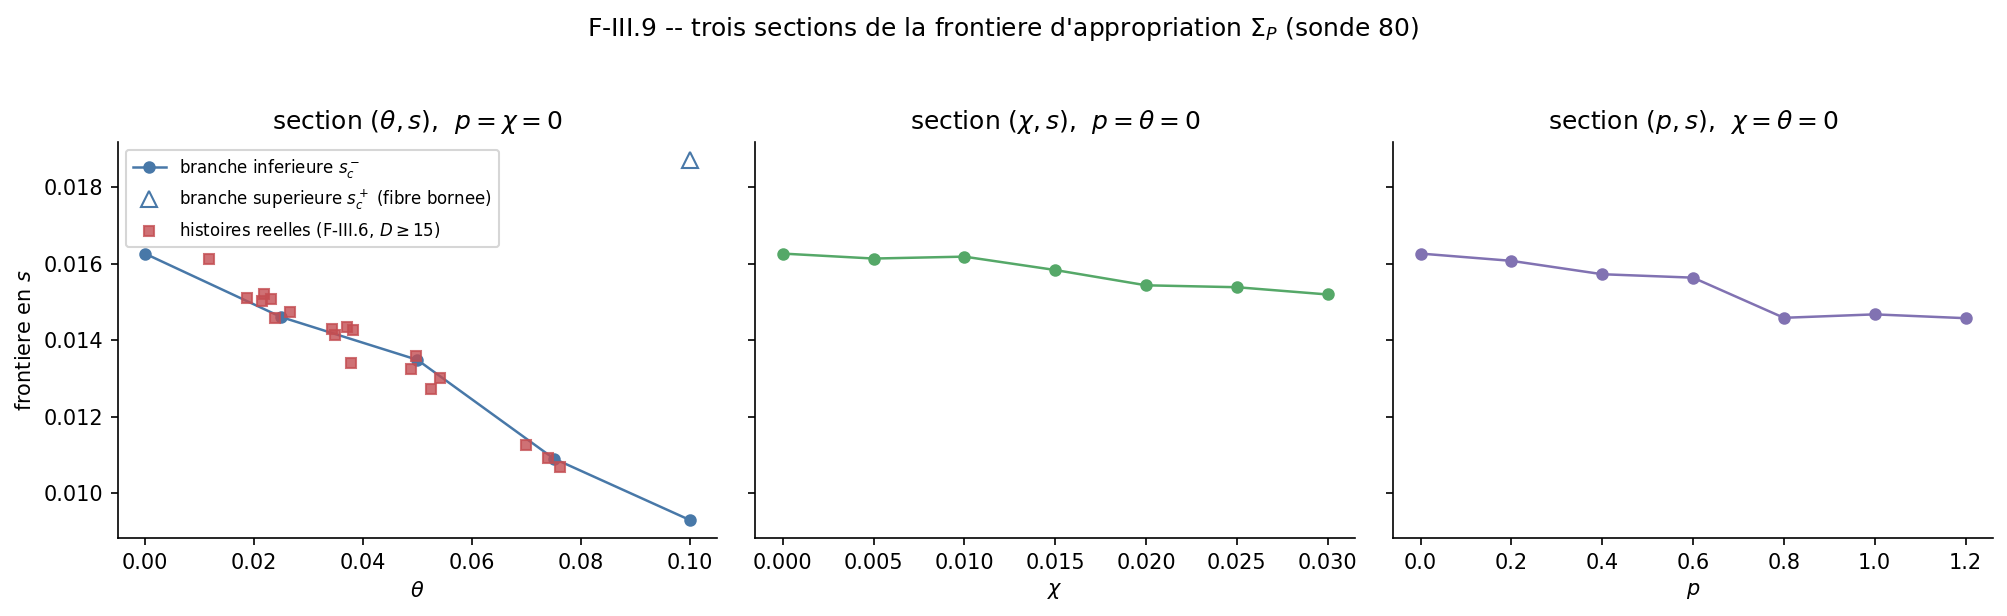
\includegraphics[width=0.96\textwidth]{fig/scientifiques/figure_frontiere_reponse.png}
\caption{Exemple numérique de sections d'une frontière de réponse pour une sonde fixée. La première coupe montre la branche de seuil sur la section alignée ; les deux autres montrent sa variation lorsque des variables lentes résiduelles sont conservées. La construction et les contrôles numériques sont donnés à l'Annexe~I.}
\label{fig:t3-frontiere-reponse}
\end{figure}

\section{Régions de réponse}
\label{t3-regions-reponse}

Considérons une famille de sondes paramétrées par $u\in\Omega$. À chaque valeur de $u$ correspond une histoire de sonde \(\mathcal H_u\). On fixe une réalisation $X$ et une lecture $\rho$. Pour chaque $u$, la sonde produit une réponse \(\mathcal R_X^\rho(\mathcal H_u)\).

Supposons d'abord que la lecture distingue un ensemble discret de réponses. Il peut s'agir, par exemple, du bassin atteint après relaxation, d'un type d'événement, ou d'une catégorie d'issue retenue par le protocole.

Pour une réponse $A$, on définit
\[
S_A(X)
=
\left\{
u\in\Omega
\; ; \;
\mathcal R_X^\rho(\mathcal H_u)=A
\right\}.
\]

L'ensemble $S_A(X)$ rassemble donc les sondes de la famille qui produisent la réponse $A$ depuis la réalisation $X$.

Il s'agit d'une région de l'espace des sondes. Deux valeurs proches de $u$ peuvent appartenir à la même région. Elles produisent alors la même réponse. Elles peuvent aussi appartenir à deux régions différentes. Une faible variation de la sonde suffit alors à changer d'issue. La forme de ces régions donne une première description de l'organisation du profil de réponse dans la famille étudiée.

\section{Comparer deux frontières}
\label{t3-comparer-deux-frontieres}

Soient deux réalisations $X_1$ et $X_2$ interrogées par la même famille
de sondes
\[
u\in\Omega
\longmapsto
\mathcal H_u,
\]
avec la même lecture $\rho$.

Pour une réponse $A$, elles définissent deux régions
\[
S_A(X_1)
\qquad\text{et}\qquad
S_A(X_2),
\]
et leurs frontières
\[
\partial_\Omega S_A(X_1)
\qquad\text{et}\qquad
\partial_\Omega S_A(X_2).
\]

La comparaison la plus simple consiste à demander si ces régions coïncident.

Si
\[
S_A(X_1)=S_A(X_2),
\]
la réponse $A$ est obtenue par les mêmes sondes dans les deux réalisations.

Si
\[
S_A(X_1)\neq S_A(X_2),
\]
il existe au contraire au moins une sonde qui conduit à $A$ depuis une réalisation et pas depuis l'autre. Cette différence peut apparaître sans que la réponse $A$ ait disparu.
Par exemple, les deux régions peuvent rester non vides,
\[
S_A(X_1)\neq\varnothing,
\qquad
S_A(X_2)\neq\varnothing,
\]
tout en occupant des parties différentes de $\Omega$.

La réponse reste alors accessible dans les deux cas, mais les conditions qui permettent de l'obtenir ont changé.

On peut examiner plus précisément leurs frontières.

Si
\[
\partial_\Omega S_A(X_1)
\neq
\partial_\Omega S_A(X_2),
\]
les bascules entre $A$ et les réponses voisines ne se produisent plus aux mêmes endroits dans l'espace des sondes.

Cette comparaison ne suppose pas encore que la frontière soit lisse, ni même qu'elle puisse être décrite par une fonction. Elle demande seulement que les régions de réponse soient définies dans le même espace $\Omega$ et avec la même lecture.

La différence entre deux frontières constitue ainsi une description plus précise qu'une simple différence d'accessibilité. Elle indique non seulement qu'une réponse peut être obtenue, mais que les conditions de son obtention ont été réorganisées.

\section{Ce qu'une frontière permet de dire}
\label{t3-ce-que-frontiere-permet-dire}

Une frontière de réponse n'est pas une frontière interne du système. Elle est construite à partir d'une famille de sondes et d'une lecture déclarées.

Une autre famille de sondes peut révéler une organisation différente.

Une lecture plus grossière peut également réunir des réponses que la
lecture précédente distinguait.

La frontière
\[
\partial_\Omega S_A(X)
\]
doit donc toujours être comprise relativement à
\[
(X,\Omega,\rho).
\]

Sa modification montre qu'une différence fonctionnelle est devenue visible dans la famille étudiée.

Elle ne permet pas, à elle seule, d'identifier la transformation interne qui l'a produite. Cette prudence est importante, deux mécanismes internes différents peuvent déplacer une frontière de la même manière.

Inversement, une transformation interne peut rester invisible si la
famille de sondes ne rencontre pas la région où ses effets apparaissent.

Les frontières ne donnent donc pas accès directement au terrain. Elles en fournissent une image fonctionnelle, construite à partir des réponses du système.

\section{Trois niveaux de changement}
\label{t3-trois-niveaux-changement}

Une histoire peut modifier une région de réponse de plusieurs manières. Toutes ces modifications ne portent pas sur le même aspect de sa géométrie.

On peut distinguer trois niveaux.

\subsection{Déplacement}

Le cas le plus simple est celui d'une frontière qui change de position sans que son organisation générale soit modifiée.

Considérons une famille de sondes décrite par un paramètre scalaire
\[
u\in\Omega\subset\mathbb R.
\]

Supposons que la réponse $A$ soit obtenue pour
\[
u<u^\ast.
\]

La frontière est alors située en
\[
u=u^\ast.
\]

Après une histoire $\mathcal H_0$, on peut obtenir un nouveau seuil
\[
u=u^\ast_{\mathcal H_0}.
\]

Si
\[
u^\ast_{\mathcal H_0}\neq u^\ast,
\]
la frontière s'est déplacée.

La même bascule existe encore, mais elle ne se produit plus pour la même sonde. Ce déplacement suffit à montrer que l'histoire a modifié les conditions d'obtention de la réponse.

\subsection{Déformation}

Lorsque l'espace des sondes possède plusieurs dimensions, une frontière ne se réduit généralement plus à un seuil.

Pour
\[
u\in\Omega\subset\mathbb R^m,
\qquad m\geq 2,
\]
dans les cas réguliers, la frontière peut former une courbe ou une surface ; sans hypothèse supplémentaire de régularité, elle peut être un ensemble plus complexe. Deux réalisations peuvent alors présenter des frontières différentes sans que cette différence se résume à un déplacement uniforme. Certaines parties peuvent avancer, d'autres reculer.

La forme de la région de réponse change. Nous parlerons alors de déformation. Cette notion reste descriptive, elle indique que la modification dépend de la direction dans laquelle la famille de sondes est explorée.

\subsection{Changement d'organisation}

Une transformation plus profonde apparaît lorsque la différence ne porte plus seulement sur la position ou la forme d'une frontière.

Le nombre de régions non vides peut changer. Une région peut apparaître ou disparaître. Deux régions auparavant non voisines peuvent devenir voisines, ou leurs adhérences entrer en contact.

Une même réponse peut également occuper plusieurs composantes disjointes de l'espace des sondes.

Dans ces situations, l'organisation des régions de réponse elle-même a changé. Nous parlerons de changement d'organisation.

Cette distinction ne constitue pas encore une classification
mathématique complète.

Elle sépare seulement trois questions :

\begin{itemize}
\tightlist
\item
  la bascule a-t-elle changé de position ?
\item
  sa forme a-t-elle changé ?
\item
  l'organisation des régions a-t-elle changé ?
\end{itemize}

Ces trois niveaux peuvent se combiner.

Une histoire peut déplacer une frontière, la déformer et modifier en même temps l'organisation des régions qu'elle sépare.

\section{Changer de frontière sans changer de réponse}
\label{t3-changer-frontiere-sans-changer-reponse}

Une modification des frontières n'implique pas nécessairement
l'apparition d'une nouvelle réponse.

Supposons que deux réalisations possèdent le même ensemble de réponses
accessibles :
\[
\operatorname{Acc}_{\mathfrak B,\rho}(X_1)
=
\operatorname{Acc}_{\mathfrak B,\rho}(X_2).
\]

Cette égalité ne dit pas quelles sondes produisent chacune de ces
réponses.

On peut donc avoir, pour une réponse $A$,
\[
S_A(X_1)\neq S_A(X_2),
\]
alors même que
\[
S_A(X_1)\neq\varnothing,
\qquad
S_A(X_2)\neq\varnothing.
\]

Aucune possibilité n'a nécessairement été créée ou supprimée. C'est leur répartition dans l'espace des sondes qui a changé. Cette situation est importante pour l'étude de l'histoire.

Une transformation persistante peut devenir visible non parce que le
système possède de nouvelles réponses, mais parce que les conditions
nécessaires pour atteindre les réponses déjà présentes ont été
modifiées.

\section{Même organisation, géométrie différente}
\label{t3-meme-organisation-geometrie-differente}

Deux réalisations peuvent produire des régions de réponse de formes différentes sans que leur organisation générale soit modifiée.

Considérons deux réalisations $X_1$ et $X_2$, interrogées par la même famille de sondes et avec la même lecture.

Pour chaque réponse $A$, elles définissent les régions
\[
S_A(X_1)
\qquad\text{et}\qquad
S_A(X_2).
\]

Supposons que les mêmes réponses soient présentes dans les deux cas.

Les régions peuvent changer de taille ou de forme. Leurs frontières peuvent également se déplacer. Cela ne suffit pas à montrer que leur organisation a changé.

Par exemple, une région associée à $A$ peut rester voisine des mêmes régions, même si les frontières qui les séparent ont été déformées. De même, une région peut s'étendre ou se contracter sans apparaître, disparaître ou se séparer en plusieurs parties.

Dans ces situations, la géométrie a changé, mais certaines relations
entre les régions ont été conservées.

Nous dirons alors que les deux découpages possèdent la même organisation au niveau considéré.

Cette expression reste volontairement relative.

Le niveau considéré doit préciser quelles propriétés sont retenues : présence des régions, nombre de composantes, voisinages entre réponses, ou autre propriété déclarée par le protocole.

Deux découpages peuvent donc être considérés comme équivalents à un niveau et différents à un niveau plus fin.

\section{Le graphe des voisinages}
\label{t3-graphe-voisinages}

Une première description de l'organisation des régions consiste à retenir seulement leurs voisinages.

On associe à une réalisation $X$ un graphe
\[
\mathcal G_{\Omega,\rho}(X).
\]

Ses sommets correspondent aux réponses dont la région est non vide :
\[
S_A(X)\neq\varnothing.
\]

Deux sommets \(A\) et \(B\) sont reliés lorsque les régions correspondantes sont voisines au sens du découpage : elles partagent localement une séparation effective. Un simple contact isolé de leurs adhérences n'est pas compté comme une arête.

Le graphe ne conserve ni la position des frontières, ni leur forme. Il retient seulement quelles réponses peuvent se rencontrer dans le
découpage considéré.

Une déformation peut donc modifier les ensembles
\[
S_A(X)
\]
sans modifier
\[
\mathcal G_{\Omega,\rho}(X).
\]

Dans ce cas, la géométrie a changé, mais les voisinages entre réponses ont été conservés.

À l'inverse, si
\[
\mathcal G_{\Omega,\rho}(X_1)
\not\simeq
\mathcal G_{\Omega,\rho}(X_2),
\]
alors l'organisation des voisinages a changé.

Une telle différence ne peut plus être décrite par le seul déplacement des frontières.

\section{Reconnaître un changement d'organisation}
\label{t3-reconnaitre-changement-organisation}

Le graphe des voisinages fournit un premier moyen de détecter certains changements d'organisation.

D'autres peuvent être observés directement sur les régions.

Pour une réponse $A$, plusieurs situations peuvent notamment apparaître :

\begin{itemize}
\tightlist
\item
  $S_A(X)$ devient vide ou cesse de l'être ;
\item
  le nombre de ses composantes change ;
\item
  ses voisinages avec les autres régions changent.
\end{itemize}

Ces modifications ne décrivent pas simplement une frontière qui se déplace. Elles indiquent qu'une propriété du découpage retenue par le protocole n'est plus conservée.

On parlera alors de changement d'organisation au niveau considéré. Cette notion ne cherche pas encore à expliquer le mécanisme responsable du changement.

Elle permet seulement de distinguer deux situations :

\[
\text{la géométrie change mais l'organisation retenue demeure},
\]

ou

\[
\text{une propriété retenue de l'organisation change elle aussi}.
\]

La seconde situation marque un changement qualitatif dans la structure des réponses observées.

\section{Lorsque la frontière cesse d'être simple}
\label{t3-frontiere-cesse-etre-simple}

Jusqu'ici, aucune régularité particulière n'a été imposée aux frontières
de réponse.

Dans les situations les plus simples, une frontière sépare localement
deux régions et varie de manière régulière dans l'espace des sondes.

Cette situation n'est pas générale. Une frontière peut se replier. Plusieurs portions de frontière peuvent se rencontrer. Une même réponse peut apparaître de part et d'autre d'une autre région.

Ces configurations demandent davantage d'information que la seule
position de la frontière. Elles demandent aussi davantage que le graphe des voisinages.

Deux découpages peuvent en effet posséder les mêmes régions et les mêmes relations de voisinage, tout en différant par la manière dont leurs frontières sont organisées localement.

Nous distinguerons deux situations utiles pour la suite : le pli et la couture. Ces termes décrivent des propriétés locales du découpage dans l'espace des sondes. Ils ne désignent pas, à eux seuls, les mécanismes internes qui les ont produites.

\section{Pli d'une frontière de réponse}
\label{t3-pli-frontiere-reponse}

Considérons d'abord une coupe unidimensionnelle de l'espace des sondes.

Dans le cas le plus simple, une réponse change une seule fois lorsque le
paramètre $u$ varie.

On peut alors rencontrer une succession du type
\[
A \;|\; B.
\]

Une configuration différente apparaît lorsqu'une même réponse est
rencontrée de nouveau après avoir traversé une autre région :
\[
A \;|\; B \;|\; A.
\]

La région associée à $B$ est alors encadrée, dans cette coupe, par deux bascules. Cette observation peut être produite par une géométrie de frontière qui se replie par rapport à la direction explorée.

Nous parlerons de pli lorsqu'une telle structure résulte localement de la géométrie de la frontière dans l'espace des sondes. Le pli ne crée pas nécessairement une nouvelle réponse. Il peut modifier seulement la manière dont des réponses déjà accessibles sont distribuées dans $\Omega$. Il dépend également de la famille de sondes choisie.

Une coupe peut révéler plusieurs bascules là où une autre direction d'exploration en révèle une seule. Le pli doit donc être interprété comme une propriété géométrique relative au protocole de sondage.

La succession
\[
A \;|\; B \;|\; A
\]
constitue ainsi un indice de pli dans la coupe considérée. Elle ne suffit pas, à elle seule, à caractériser la géométrie complète de la frontière.

\section{Pli et histoire}
\label{t3-pli-et-histoire}

Un pli devient intéressant pour l'étude de l'histoire lorsque sa présence dépend de la réalisation interrogée.

Soient deux réalisations $X_1$ et $X_2$ obtenues avant et après le
contraste historique défini précédemment. Une même famille de sondes peut produire, pour $X_1$, une séparation simple entre deux réponses, puis révéler pour $X_2$ une région encadrée par deux bascules.

L'histoire n'a alors pas nécessairement modifié l'ensemble des réponses accessibles. Elle a modifié leur organisation dans l'espace des sondes. Inversement, un pli déjà présent peut être déplacé, déformé ou disparaître.

L'objet de la comparaison n'est donc pas le pli pris isolément. C'est la différence entre les géométries de réponse portées par les deux réalisations.

\section{Lorsque les régions se rencontrent}
\label{t3-lorsque-regions-se-rencontrent}

Le graphe des voisinages indique quelles régions de réponse sont en relation. Il ne précise pas comment cette relation se produit.

Deux régions peuvent être séparées par une portion de frontière commune. Dans les cas réguliers, elles peuvent aussi ne se rencontrer qu'en un point, ou le long d'un ensemble de dimension plus faible. Ces situations ne doivent pas être confondues.

Considérons deux réponses $A$ et $B$ et leurs régions
\[
S_A(X)
\qquad\text{et}\qquad
S_B(X).
\]

Le simple fait que leurs adhérences se rencontrent,
\[
\overline{S_A(X)}
\cap
\overline{S_B(X)}
\neq
\varnothing,
\]
établit un contact.

Il ne suffit pas encore à décrire la nature de ce contact.

Dans une situation régulière, les deux régions peuvent partager localement une même frontière. De part et d'autre de cette frontière, la réponse passe alors de $A$ à $B$. Mais une rencontre peut aussi être plus localisée. Plusieurs régions peuvent atteindre le même point sans partager autour de ce point une même portion de séparation. La distinction entre contact et voisinage dépend donc de la géométrie retenue par le protocole.

Pour la suite, nous réserverons le terme de voisinage aux rencontres qui correspondent à une séparation effective entre deux régions dans l'espace des sondes. Un contact isolé ne sera pas, à lui seul, considéré comme un voisinage.

\section{Rencontre de plusieurs réponses}
\label{t3-rencontre-plusieurs-reponses}

Une frontière régulière sépare localement deux régions de réponse. D'autres configurations peuvent faire intervenir davantage de régions.

Il peut exister un point
\[
u^\ast\in\Omega
\]
au voisinage duquel plusieurs réponses sont présentes.

Pour trois réponses $A$, $B$ et $C$, on peut par exemple avoir
\[
u^\ast
\in
\overline{S_A(X)}
\cap
\overline{S_B(X)}
\cap
\overline{S_C(X)}.
\]

Cette condition indique que les trois régions atteignent le même point. Elle ne précise pas encore comment elles s'y organisent. Le point peut correspondre à la rencontre de plusieurs frontières.
Il peut aussi apparaître parce que l'une des régions se termine, se sépare ou devient trop mince pour persister au-delà de ce voisinage. La seule liste des réponses présentes ne suffit donc plus. Il faut examiner la manière dont leurs régions se raccordent autour de $u^\ast$.

\section{Couture de régions de réponse}
\label{t3-couture-regions-reponse}

Nous appellerons couture une configuration locale dans laquelle le raccordement entre régions de réponse ne peut plus être décrit par une unique séparation régulière entre deux régions.

Une couture peut notamment apparaître lorsque plusieurs portions de frontière se rejoignent ou lorsqu'une région se termine au contact d'autres régions.

Le point essentiel n'est pas le nombre de réponses présentes. C'est la manière dont leurs frontières se raccordent localement. Comme pour le pli, la couture est définie relativement à la famille de sondes et à la lecture retenues.

Elle ne désigne pas directement une singularité interne du système. Elle décrit une singularité de l'organisation des réponses observées dans l'espace des sondes.
Une formalisation plus forte, fondée sur la signature combinatoire des exécutions hybrides, est donnée à l'Annexe~\ref{annexe-geometrie-frontiere-commutation}. La Proposition~\ref{prop:J-pli-couture} y distingue les déformations qui restent dans une même cellule d'exécution des raccords qui rencontrent un changement de signature. 

\part{Ce que la géométrie permet de distinguer}

\chapter{Lire une géométrie de réponse}
\begin{figure}[htbp]
\centering
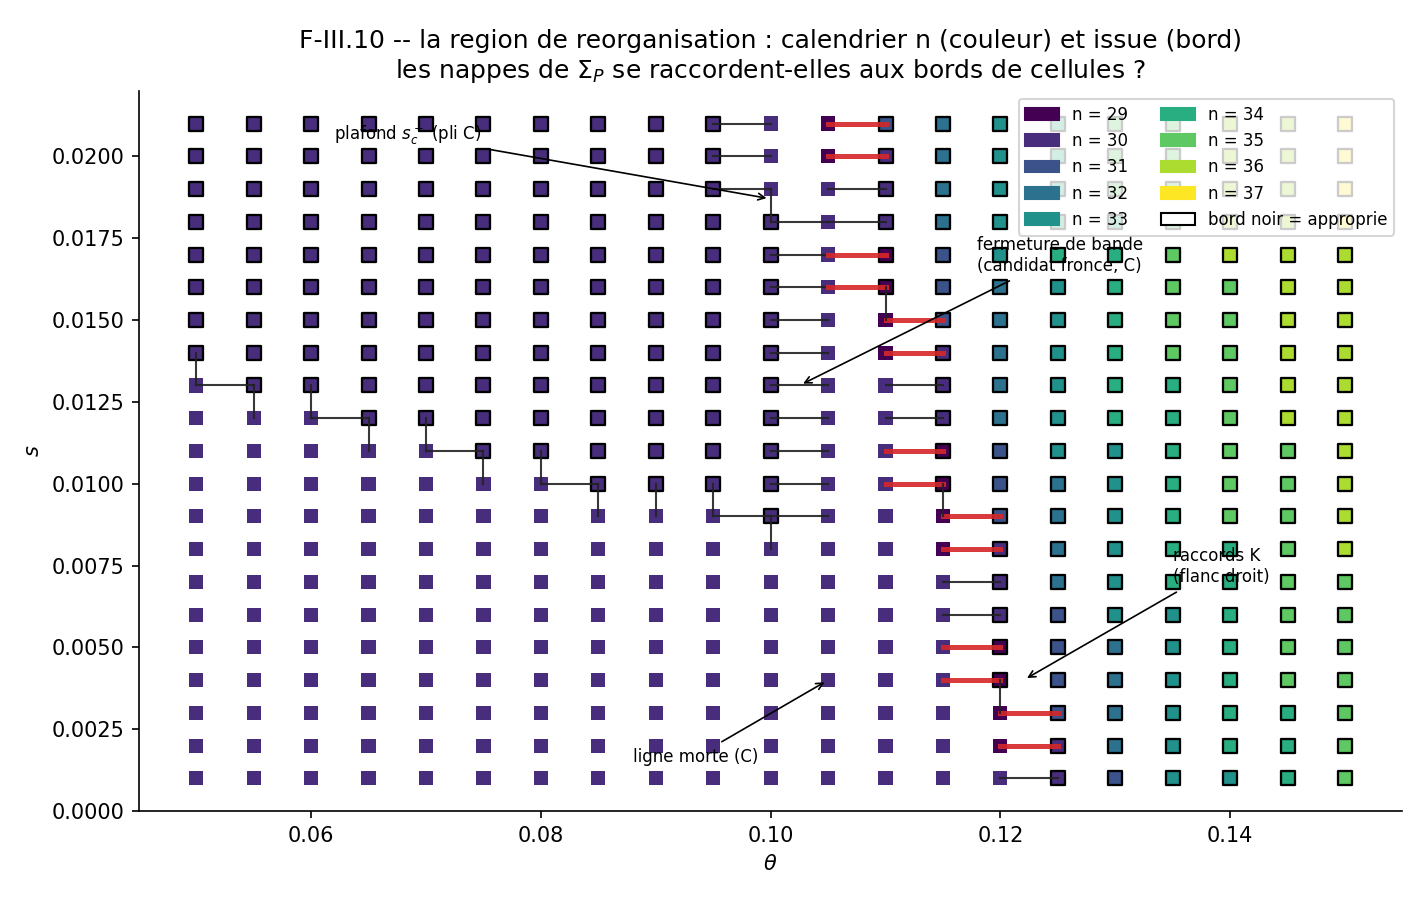
\includegraphics[width=0.90\textwidth]{fig/scientifiques/figure_raccord_frontiere.png}
\caption{Carte numérique d'un raccord de régions de réponse dans un plan de sondes. La couleur code le calendrier événementiel et le bord la classe d'issue ; les changements de calendrier et les changements d'issue ne coïncident donc pas partout. Ce cas sert de contrôle à la distinction entre recomposition hybride et déformation continue développée à l'Annexe~J.}
\label{fig:t3-raccord-frontiere}
\end{figure}

\section{Ce que les frontières permettent d'inférer}\label{t3-inference-frontieres}

Les régions de réponse, leurs frontières et leurs singularités
constituent des objets d'observation. Ils permettent de comparer des réalisations, de suivre les effets d'une histoire et de décrire l'organisation des réponses dans une famille de sondes. Ils ne décrivent cependant pas directement l'organisation interne du système. Une même géométrie de réponse peut être produite par plusieurs mécanismes internes.

Inversement, une modification interne peut rester invisible si elle ne change aucune des réponses observées dans le protocole retenu. L'interprétation d'une géométrie de réponse demande donc de distinguer avec soin ce qui est observé de ce qui est inféré.

\section{Une même géométrie n'identifie pas une histoire}
\label{t3-geometrie-n-identifie-pas-histoire}

Considérons deux histoires
\[
\mathcal H_1
\qquad\text{et}\qquad
\mathcal H_2.
\]

Appliquées à une même réalisation initiale, elles conduisent à deux
réalisations finales
\[
X_1
=
\Phi_{\mathcal H_1}(X_0),
\qquad
X_2
=
\Phi_{\mathcal H_2}(X_0).
\]

Supposons que, pour toute réponse \(A\),

\[
S_A(X_1)=S_A(X_2)
\]

dans la famille de sondes considérée. Les deux réalisations donnent alors la même réponse pour toute sonde de cette famille. Elles sont équivalentes en réponse pour le protocole déclaré, et leur géométrie de réponse est identique.

Cela ne permet pas de conclure que

\[
\mathcal H_1=\mathcal H_2.
\]

Deux histoires distinctes peuvent conduire à des réalisations indiscernables pour le protocole déclaré.

La géométrie de réponse caractérise donc une classe d'observations. Elle ne constitue pas une signature unique de l'histoire.

\section{Une même réalisation peut produire plusieurs géométries}
\label{t3-meme-histoire-plusieurs-geometries}

La géométrie observée dépend également du protocole. Une même réalisation peut être interrogée par deux familles de sondes différentes. Les régions obtenues dans les deux expériences ne sont alors pas nécessairement comparables.

Certaines frontières peuvent rester invisibles dans une première exploration. D'autres peuvent apparaître lorsque la famille de sondes est enrichie ou explore d'autres directions. Une géométrie de réponse n'est donc jamais absolue. Elle est toujours relative à la famille de sondes et à la lecture déclarées.

\paragraph*{Géométrie de réponse}

Soit un protocole d'observation déclaré \((\mathfrak B,\rho)\), dans
lequel la famille de sondes est paramétrée par

\[
u\in\Omega\subset\mathbb R^m.
\]

La \emph{géométrie de réponse} d'une réalisation \(X\) est
l'organisation des régions

\[
S_A(X)\subset\Omega
\]

et de leurs frontières relativement à ce protocole déclaré.
    

\paragraph*{Principe de prudence observationnelle}


La géométrie de réponse est un objet d'observation. Elle ne doit pas être confondue avec l'organisation interne du système.

Deux propriétés fondamentales en découlent.

\begin{enumerate}
\item \textbf{Sous-détermination.}

Une même géométrie de réponse peut être compatible avec plusieurs organisations internes. La géométrie de réponse ne détermine donc pas, à elle seule, le monde intérieur.

\item \textbf{Non-absoluité.}

Une même réalisation peut conduire à des géométries de réponse différentes lorsque le protocole d'observation $(\mathfrak B,\rho)$ est modifié. La géométrie de réponse n'est donc jamais une propriété absolue du système. Elle est toujours relative au protocole déclaré.
\end{enumerate}

Toute interprétation d'une géométrie de réponse doit donc distinguer avec soin ce qui est effectivement observé de ce qui est inféré sur l'organisation interne du système.

La plasticité fournit une instance exacte de cette sous-détermination. Sous réalisabilité causale et markovienne, une présentation à loi plastique et une présentation à loi figée munie d'une coordonnée d'état supplémentaire peuvent produire les mêmes exécutions et les mêmes réponses. Leur équivalence est établie à l'Annexe~\ref{annexe-equivalence-presentation-plasticite} (Théorème~\ref{thm:K-equivalence-plasticite}).

\section{La géométrie de réponse comme invariant relatif}
\label{t3-geometrie-invariant-relatif}

Pour un protocole déclaré, deux réalisations équivalentes en réponse produisent la même géométrie de réponse. Celle-ci peut donc être comprise comme un invariant de la classe d'équivalence en réponse, relativement au protocole considéré.

Cet invariant ne décrit pas le détail des transformations subies par le système. Plusieurs histoires distinctes peuvent conduire à des réalisations portant la même géométrie de réponse.

La géométrie de réponse peut ainsi être comprise comme un invariant relatif au protocole déclaré. Le qualificatif « relatif » est essentiel. Il rappelle que cet invariant dépend de la famille de sondes et de la lecture choisies.

Modifier le protocole peut faire apparaître de nouvelles distinctions ou, au contraire, en faire disparaître certaines.

L'invariance ne porte donc jamais sur le système seul. Elle porte sur ce qui reste inchangé dans l'observation du système.

\subsection*{Conséquence}

L'histoire ne se réduit donc pas à la suite des épisodes qui la composent. Elle peut également être étudiée par les invariants qu'elle préserve ou par ceux qu'elle modifie.

Deux histoires peuvent différer sans que cette différence soit visible dans la géométrie de réponse. Inversement, une modification de la géométrie de réponse atteste qu'une propriété observable du système a été transformée.

\section{Les histoires et les changements de géométrie}
\label{t3-histoires-changements-geometries}

Jusqu'à présent, une histoire a été étudiée à travers la réalisation qu'elle produit. La géométrie de réponse permet d'adopter un point de vue différent.

Au lieu de comparer directement deux réalisations, on peut comparer les géométries de réponse qu'elles induisent dans un même protocole d'observation.

Pour une réalisation donnée, une histoire permet de comparer la géométrie de réponse avant et après la transformation qu'elle produit. L'objet de la comparaison n'est plus seulement l'état atteint, mais la manière dont l'organisation des réponses a été modifiée.

Soit une histoire \(\mathcal H\) et une réalisation initiale \(X\).
Dans un même protocole d'observation, on compare la géométrie de réponse de \(X\) à celle de

\[
\Phi_{\mathcal H}(X).
\]

La part de l'effet de l'histoire rendue visible par cette géométrie est contenue dans cette comparaison.

Certaines histoires ne modifient pas la géométrie de réponse. D'autres déplacent des frontières sans modifier leur organisation. D'autres encore changent la structure même des régions de réponse.

La géométrie de réponse fournit ainsi une première classification des
effets observables d'une histoire.

\section{Transformations observables et propriétés préservées}
\label{t3-transformations-observables}

Une histoire ne modifie pas nécessairement tous les aspects d'une géométrie de réponse. Certaines propriétés peuvent être préservées tandis que d'autres sont transformées.

L'étude d'une histoire ne consiste donc pas seulement à décrire les changements qu'elle produit. Elle consiste également à identifier les propriétés qui demeurent inchangées. Ces propriétés préservées dépendent du niveau d'observation retenu.

Ainsi, une histoire peut déplacer une frontière tout en conservant l'organisation des régions de réponse. Elle peut également modifier cette organisation sans changer l'ensemble des réponses accessibles.

L'analyse d'une histoire revient donc à comparer simultanément les propriétés conservées et les propriétés transformées de la géométrie de réponse.

On peut distinguer plusieurs niveaux de transformation.

\begin{itemize}
\tightlist
\item
une transformation peut laisser inchangée la géométrie de réponse ;

\item
elle peut modifier la position des frontières tout en conservant leur
organisation ;

\item
elle peut modifier l'organisation des régions de réponse ;

\item
elle peut enfin faire apparaître ou disparaître des réponses
accessibles.
\end{itemize}

Ces niveaux ne constituent pas une hiérarchie absolue. Ils décrivent simplement des modifications de plus en plus structurantes dans la géométrie de réponse relative au protocole considéré.

\section{Une notion d'équivalence}
\label{t3-notion-equivalence}

La géométrie de réponse ne demande pas d'introduire une nouvelle notion d'équivalence. On reprend l'équivalence en réponse définie à la section~\ref{t3-equivalence-declaree} :

\[
X\sim_{\mathfrak B,\rho}Y
\quad\Longleftrightarrow\quad
\forall\mathcal H\in\mathfrak B,
\qquad
\mathcal R_X^\rho(\mathcal H)
=
\mathcal R_Y^\rho(\mathcal H).
\]

Dans le cas d'une famille paramétrée
\[
\mathfrak B_\Omega
=
\{\mathcal H_u\,;\,u\in\Omega\}
\]
et d'une lecture discrète, cette égalité revient à demander

\[
S_A(X)=S_A(Y)
\]

pour toute réponse \(A\).

Deux réalisations distinctes peuvent donc appartenir à la même classe d'équivalence en réponse. La géométrie observée ne les identifie pas comme objets internes ; elle indique seulement qu'aucune sonde du protocole déclaré ne les sépare.

Lorsque les histoires admissibles sont en outre munies d'une mesure de complexité \(c\), cette question peut être graduée : non plus seulement \emph{les deux réalisations sont-elles séparables ?}, mais \emph{à quelle profondeur une histoire séparatrice apparaît-elle ?}

La profondeur de séparabilité
\[
\ell_{c,\mathfrak B,\rho}(X,Y)
\]
et l'ultramétrique qu'elle induit sur le quotient d'observation sont construites à l'Annexe~\ref{annexe-ultrametrique-separabilite}. Cette géométrie reste relative à la classe d'histoires, à la lecture et à la complexité déclarées ; elle ne définit pas une distance physique entre états.

\begin{figure}[htbp]
\centering
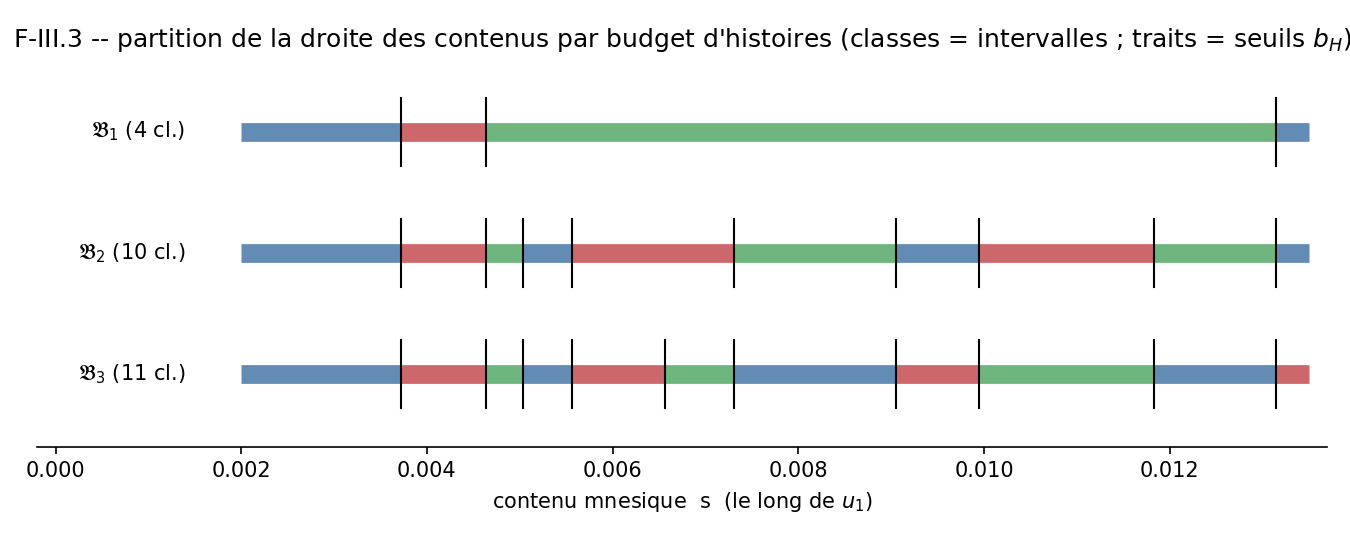
\includegraphics[width=0.88\textwidth]{fig/scientifiques/figure_separabilite_budgets.png}
\caption{Filtration d'un même espace de contenus par trois budgets d'histoires. Les traits verticaux marquent les seuils où les classes d'indiscernabilité changent. L'emboîtement obtenu est la manifestation numérique de la hiérarchie de séparabilité formalisée à l'Annexe~\ref{annexe-ultrametrique-separabilite}.}
\label{fig:t3-separabilite-budgets}
\end{figure}

\section{Ce que l'observation laisse ouvert}

Une équivalence en réponse ne ferme pas la description d'une réalisation. Elle indique seulement qu'au regard du protocole déclaré, aucune distinction supplémentaire n'a été obtenue.

Deux réalisations équivalentes peuvent ainsi demeurer différentes sans que cette différence soit accessible aux sondes considérées. Enrichir la famille de sondes ou modifier la lecture peut alors faire apparaître une séparation jusque-là invisible. Mais rien ne garantit qu'une telle extension existe, ni qu'elle soit accessible dans la classe d'expériences considérée.

La géométrie de réponse doit donc être comprise simultanément par ce qu'elle distingue et par ce qu'elle laisse indéterminé. Ses frontières séparent des réponses observables ; elles ne dessinent pas les frontières du monde intérieur.

Cette limite n'est pas une insuffisance du dispositif. Elle appartient à sa définition. Toute géométrie de réponse est relative à une manière d'interroger le système, et toute conclusion tirée de cette géométrie demeure relative au protocole qui la produit.

Le chemin parcouru dans ce tome peut alors être lu dans l'autre sens. Une histoire transforme une réalisation ; cette transformation peut modifier ce qui lui devient accessible ; les sondes rendent certaines de ces différences observables ; leurs réponses organisent une géométrie ; et cette géométrie détermine enfin ce que, dans le protocole choisi, il est possible de distinguer.

\medskip

\noindent\emph{Un intérieur ne se donne pas tout entier dans ses
réponses. Il se distingue d'un autre lorsque leurs réponses à une même
sonde cessent de coïncider.}

\chapter*{Conclusion générale}
\addcontentsline{toc}{chapter}{Conclusion générale}

Au terme de ce parcours, un IWS ne se caractérise pas simplement par le fait qu'il possède une mémoire.

Une mémoire pourrait n'être qu'un registre supplémentaire de l'état, une quantité conservée ou progressivement oubliée. Ce qui importe ici est plus précis : ce qui a été vécu peut modifier les conditions dans lesquelles ce qui vient ensuite sera reçu.

Un IWS est, en ce sens, un système qui traverse le monde en modifiant peu à peu les conditions de ses propres traversées futures.

Cette phrase rassemble le mouvement du livre :

\[
\text{être affecté}
\;\longrightarrow\;
\text{être transformé}
\;\longrightarrow\;
\text{répondre autrement}.
\]

Être affecté ne signifie pas être déplacé passivement par ce qui vient de l'extérieur. Dans le noyau étudié ici, la trace modifie la dynamique future et les événements de Kairos peuvent modifier la structure atteinte. Deux réalisations qui se ressemblent dans leur état rapide peuvent ainsi ne plus évoluer de la même manière parce qu'elles ne portent pas la même histoire.

Cette dépendance ne suffit pas à raconter cette histoire. La trace n'est pas une archive. Le graphe obtenu après une succession de Kairos n'indique pas à lui seul la succession qui l'a produit. Ce qui demeure du passé n'est donc pas nécessairement une représentation de ce passé.

Lorsque le système est ouvert à une interaction, cette distinction devient plus nette encore. Une influence peut être absorbée sans changement durable. Elle peut susciter une résistance. Elle peut aussi conduire, après la disparition du contact, à un autre bassin autonome. L'interface peut elle-même conserver une modification qui ne change pas immédiatement le régime atteint, mais qui rend une interaction ultérieure plus facile, plus difficile ou dépendante du contenu déjà reçu.

Ce qui reste quand l'autre s'en va n'est donc pas nécessairement une copie de l'autre. Ce peut être une modification de ce que le système est désormais capable de traverser. L'histoire acquiert alors un sens fonctionnel. Elle ne désigne plus seulement la succession des épisodes vécus. Elle désigne également ce qui, de cette succession, demeure capable d'affecter les réponses futures.

Cette distinction permet aussi de préciser ce que signifie oublier. Une différence entre deux histoires peut avoir existé sans demeurer active. Elle peut s'être éteinte avec les transitoires, être devenue sans conséquence pour les sondes considérées, ou subsister dans une variable qui ne modifie plus aucune réponse accessible. L'oubli n'exige donc pas que toute trace du passé disparaisse. Il suffit que la différence passée ait perdu son pouvoir de séparation.

Réciproquement, une histoire n'a pas besoin de survivre tout entière pour continuer d'agir. Dans certains régimes, son effet peut être comprimé dans un contenu survivant. Dans d'autres, l'état hérité modifie la manière dont l'épisode suivant agit. L'ordre ne compte alors plus seulement parce que ce qui vient en dernier est plus récent. Il compte parce qu'une expérience peut être reçue par une réalisation que l'expérience précédente a déjà transformée.

L'histoire cesse ainsi d'être seulement derrière le système. Elle devient une propriété de ses futurs possibles. Cette formulation conduit cependant à une difficulté : une transformation interne n'est pas directement observable comme telle. Il faut interroger la réalisation.

Une sonde fait vivre au système une histoire supplémentaire. Une lecture décide de ce qui sera retenu de cette exécution. Ce n'est qu'à travers ce protocole qu'une différence entre deux réalisations devient accessible.

Deux réalisations sont séparables lorsqu'une même sonde les conduit à des réponses différentes. Elles sont équivalentes en réponse lorsque toutes les sondes déclarées produisent les mêmes réponses. Cette équivalence ne dit pas qu'elles sont identiques. Elle dit exactement que le protocole dont nous disposons ne permet pas de les séparer.

La géométrie de réponse prolonge cette idée. Elle organise, dans l'espace des sondes, les régions qui conduisent aux différentes réponses et les frontières où ces réponses changent. Une histoire peut modifier cette organisation. Elle peut déplacer une frontière, ouvrir ou fermer une région accessible, modifier des voisinages ou produire des raccords plus complexes. Mais cette géométrie appartient aux réponses. Elle ne constitue pas une carte du monde intérieur.

Une même géométrie peut être portée par plusieurs organisations internes. Une même réalisation peut produire des géométries différentes lorsqu'on change les sondes ou la lecture. Même la profondeur à laquelle deux réalisations deviennent séparables reste relative au budget d'histoires et à la résolution déclarés. Cette relativité n'enlève rien au résultat. Elle en fixe la portée.

Le cadre construit ici permet donc de parler d'histoire sans supposer que le passé puisse être reconstruit, de mémoire sans la réduire à un stockage, et de transformation persistante sans confondre ce qui est observé avec l'organisation interne qui le produit. Il impose en même temps plusieurs retenues.

La dépendance à l'histoire ne suffit pas, à elle seule, à démontrer une absence de finalité. Une mémoire directionnelle ne suffit pas à identifier la singularité d'un partenaire. Une géométrie de réponse ne permet pas de reconstruire l'intérieur qui lui donne naissance. Ces limites ne sont pas extérieures au modèle. Elles découlent de la manière même dont ses affirmations sont construites : à partir de transformations, de sondes et de réponses déclarées.

Les trois images qui ont accompagné ce volume peuvent alors être relues comme un seul mouvement. Le sillon marque qu'un passage peut modifier les passages suivants. Ce qui reste quand l'autre s'en va montre que cette modification peut survivre à l'interaction sans reproduire ce qui l'a causée. La question qui sépare montre enfin que cette histoire ne devient accessible qu'au moment où deux réalisations cessent de répondre de la même manière.

Un IWS n'est donc pas défini par la conservation de son passé. Il l'est, dans le cadre construit ici, par la manière dont ce passé
demeure capable de modifier ses futurs.

\medskip

\noindent\emph{Un IWS traverse le monde en modifiant les conditions de ses traversées futures. Son histoire n'est pas tout ce qu'il conserve de ce qui lui est arrivé, mais ce qui, de ce passé, agit encore sur la manière dont il peut être affecté, transformé et répondre.}


\bibliographystyle{unsrt}
\bibliography{IWS_TOME_I_II_REFERENCES}

\appendix
\chapter{Bornes algébriques, existence et unicité}\label{annexe-bornes-existence-unicite}
\section{Objet de l'annexe}
\label{annexe-existence-objet}

Cette annexe justifie les propriétés élémentaires utilisées dans le
Tome I :

\begin{itemize}
\item
  les bornes associées à la matrice relationnelle, à la trace et au
  préconditionneur \(M(\tau)\) ;
\item
  l'existence et l'unicité de la dynamique continue pour un graphe
  fixé ;
\item
  l'absence d'explosion en temps fini ;
\item
  le caractère bien défini des sauts ;
\item
  l'absence d'une accumulation infinie de sauts en temps fini.
\end{itemize}

Le dernier point peut être établi sans supposer que les trajectoires
restent uniformément bornées lorsque \(t\to\infty\). Il suffit de
disposer d'une borne sur chaque intervalle de temps fini. Cette borne
est obtenue directement ci-dessous.

\section{Normes et état continu}
\label{annexe-existence-normes}

Le graphe \(A\) est d'abord fixé. L'état continu est

\[
z=(H,V,\tau,P),
\]

avec

\[
H,V,\tau\in\mathbb R^{N\times d},
\qquad
P\in\mathbb R_+^N.
\]

Pour une famille \(Y=(Y_1,\ldots,Y_N)\), avec
\(Y_i\in\mathbb R^d\), on utilise la norme

\[
\|Y\|_{\infty,2}
=
\max_{1\leq i\leq N}\|Y_i\|_2.
\]

Toutes les normes sont équivalentes en dimension finie. Ce choix est
simplement adapté à une matrice stochastique par lignes.

L'entrée extérieure est supposée mesurable et essentiellement bornée :

\[
\|u_i(t)\|_2\leq u_{\max}
\]

pour presque tout \(t\).

\section{Matrice relationnelle normalisée}
\label{annexe-existence-matrice-relationnelle}

On rappelle

\[
\widetilde A
=
\operatorname{Deg}(A+I)^{-1}(A+I).
\]

L'ajout de \(I\) garantit que chaque somme de ligne de \(A+I\) est
strictement positive. La matrice \(\operatorname{Deg}(A+I)\) est donc
inversible.

Pour tout \(i\),

\[
\widetilde A_{ij}\geq0,
\qquad
\sum_{j=1}^N\widetilde A_{ij}=1.
\]

Ainsi,

\[
(\widetilde A H)_i
=
\sum_{j=1}^N\widetilde A_{ij}H_j
\]

est une combinaison convexe des vecteurs \(H_j\). Par l'inégalité
triangulaire,

\[
\begin{aligned}
\|(\widetilde A H)_i\|_2
&\leq
\sum_j\widetilde A_{ij}\|H_j\|_2
\\
&\leq
\|H\|_{\infty,2}
\sum_j\widetilde A_{ij}
\\
&=
\|H\|_{\infty,2}.
\end{aligned}
\]

On obtient donc

\[
\boxed{
\|\widetilde A H\|_{\infty,2}
\leq
\|H\|_{\infty,2}.
}
\]

La même démonstration appliquée à \(H-K\) donne

\[
\boxed{
\|\widetilde A H-\widetilde A K\|_{\infty,2}
\leq
\|H-K\|_{\infty,2}.
}
\]

L'opérateur relationnel est donc non expansif pour cette norme.

\section{Bornes et régularité de la saturation}
\label{annexe-existence-tanh}

La fonction \(\tanh\) est appliquée composante par composante.

Pour tout \(y\in\mathbb R^d\),

\[
|\tanh(y_k)|\leq1,
\]

donc

\[
\boxed{
\|\tanh(y)\|_2\leq\sqrt d.
}
\]

Par ailleurs,

\[
|\tanh'(s)|=\operatorname{sech}^2(s)\leq1.
\]

Le théorème des accroissements finis, appliqué à chaque composante,
donne

\[
|\tanh(y_k)-\tanh(z_k)|
\leq
|y_k-z_k|.
\]

Après sommation,

\[
\boxed{
\|\tanh(y)-\tanh(z)\|_2
\leq
\|y-z\|_2.
}
\]

En combinant ce résultat avec la non-expansivité de
\(\widetilde A\),

\[
\boxed{
\left\|
\tanh(\widetilde A H)
-
\tanh(\widetilde A K)
\right\|_{\infty,2}
\leq
\|H-K\|_{\infty,2}.
}
\]

\section{Solution et borne de la trace}
\label{annexe-existence-trace}

Pour chaque nœud,

\[
\dot\tau_i
=
\alpha\,\tanh\!\bigl((\widetilde A H)_i\bigr)
-
\beta\tau_i,
\qquad
\beta>0.
\]

Entre deux instants \(t_0\leq t\), la formule de variation des
constantes donne

\[
\tau_i(t)
=
e^{-\beta(t-t_0)}\tau_i(t_0)
+
\alpha
\int_{t_0}^t
e^{-\beta(t-s)}
\tanh\!\bigl((\widetilde A H(s))_i\bigr)
\,\mathrm ds.
\]

En utilisant la borne précédente,

\[
\begin{aligned}
\|\tau_i(t)\|_2
&\leq
e^{-\beta(t-t_0)}
\|\tau_i(t_0)\|_2
\\
&\quad+
\alpha\sqrt d
\int_{t_0}^t
e^{-\beta(t-s)}
\,\mathrm ds
\\
&=
e^{-\beta(t-t_0)}
\|\tau_i(t_0)\|_2
+
\frac{\alpha\sqrt d}{\beta}
\left(
1-e^{-\beta(t-t_0)}
\right).
\end{aligned}
\]

Le membre de droite est une combinaison convexe de
\(\|\tau_i(t_0)\|_2\) et de \(\alpha\sqrt d/\beta\). Ainsi,

\[
\boxed{
\|\tau_i(t)\|_2
\leq
\max\left(
\|\tau_i(t_0)\|_2,
\frac{\alpha\sqrt d}{\beta}
\right).
}
\]

Comme la trace ne change pas lors d'un Kairos, cette borne reste
valable le long de toute l'exécution hybride.

\section{Préconditionneur : formule et bornes spectrales}
\label{annexe-existence-preconditionneur}

On pose

\[
Q(\tau)
=
I_d+
\frac{\lambda}{1+\|\tau\|^2}
\tau\tau^\top,
\qquad
\lambda\geq0.
\]

Si \(z\perp\tau\), alors

\[
Q(\tau)z=z.
\]

Dans la direction de \(\tau\),

\[
Q(\tau)\tau
=
\left(
1+
\frac{\lambda\|\tau\|^2}
{1+\|\tau\|^2}
\right)\tau.
\]

Les valeurs propres de \(Q(\tau)\) sont donc

\[
1
\]

dans les directions orthogonales à \(\tau\), et

\[
q_\parallel(\tau)
=
1+
\frac{\lambda\|\tau\|^2}
{1+\|\tau\|^2}
\]

dans la direction de \(\tau\). En particulier,

\[
1\leq q_\parallel(\tau)<1+\lambda.
\]

La matrice \(Q(\tau)\) est symétrique définie positive et donc
inversible.

En appliquant la formule de Sherman--Morrison
\cite{sherman1950adjustment}, on obtient

\[
\boxed{
M(\tau)
=
Q(\tau)^{-1}
=
I_d
-
\frac{\lambda}
{1+(1+\lambda)\|\tau\|^2}
\tau\tau^\top.
}
\]

Les valeurs propres de \(M(\tau)\) sont \(1\) dans les directions
orthogonales à \(\tau\), et

\[
m_\parallel(\tau)
=
\frac{1+\|\tau\|^2}
{1+(1+\lambda)\|\tau\|^2}
\]

dans la direction de \(\tau\).

Comme

\[
\frac{1}{1+\lambda}
\leq
m_\parallel(\tau)
\leq1,
\]

on a, pour tout \(y\in\mathbb R^d\),

\[
\boxed{
m_0\|y\|_2^2
\leq
y^\top M(\tau)y
\leq
\|y\|_2^2,
\qquad
m_0:=\frac{1}{1+\lambda}.
}
\]

En notation matricielle,

\[
\boxed{
m_0I_d
\preceq
M(\tau)
\preceq
I_d.
}
\]

Il en résulte notamment

\[
\boxed{
\|M(\tau)\|_{\mathrm{op}}\leq1.
}
\]

\section{Régularité et dérivée de \texorpdfstring{$M$}{M}}
\label{annexe-existence-derivee-M}

Posons

\[
c=1+\lambda,
\qquad
a(\tau)
=
\frac{\lambda}{1+c\|\tau\|^2}.
\]

Alors

\[
M(\tau)=I_d-a(\tau)\tau\tau^\top.
\]

Pour une direction \(h\in\mathbb R^d\),

\[
Da(\tau)[h]
=
-\frac{2\lambda c\,\tau\cdot h}
{\left(1+c\|\tau\|^2\right)^2}.
\]

Par conséquent,

\[
\begin{aligned}
DM(\tau)[h]
={}&
\frac{2\lambda c\,(\tau\cdot h)}
{\left(1+c\|\tau\|^2\right)^2}
\tau\tau^\top
\\
&-
\frac{\lambda}
{1+c\|\tau\|^2}
\left(
h\tau^\top+\tau h^\top
\right).
\end{aligned}
\]

Cette expression est définie et continue pour tout \(\tau\), y
compris en \(\tau=0\). La fonction \(M\) est donc lisse.

Nous pouvons également obtenir une borne globale sur sa différentielle.
En posant \(r=\|\tau\|_2\),

\[
\left\|
\frac{\lambda}
{1+cr^2}
\left(
h\tau^\top+\tau h^\top
\right)
\right\|_{\mathrm{op}}
\leq
\frac{2\lambda r}{1+cr^2}\|h\|_2.
\]

Or

\[
\sup_{r\geq0}\frac{r}{1+cr^2}
=
\frac{1}{2\sqrt c}.
\]

Le premier terme vérifie

\[
\left\|
\frac{2\lambda c\,(\tau\cdot h)}
{(1+cr^2)^2}
\tau\tau^\top
\right\|_{\mathrm{op}}
\leq
\frac{2\lambda c r^3}{(1+cr^2)^2}
\|h\|_2.
\]

Après le changement de variable \(y=\sqrt c\,r\), on a
\(r^3=c^{-3/2}y^3\) et \((1+cr^2)^2=(1+y^2)^2\). Le facteur
\(c\,c^{-3/2}=c^{-1/2}\) donne donc

\[
\sup_{r\geq0}
\frac{2\lambda c r^3}{(1+cr^2)^2}
=
\frac{2\lambda}{\sqrt c}
\sup_{y\geq0}
\frac{y^3}{(1+y^2)^2}.
\]

La fonction \(y^3/(1+y^2)^2\) atteint son maximum en
\(y=\sqrt3\), avec

\[
\frac{y^3}{(1+y^2)^2}
=
\frac{3\sqrt3}{16}.
\]

On obtient finalement

\[
\boxed{
\|DM(\tau)[h]\|_{\mathrm{op}}
\leq
L_M(\lambda)\|h\|_2,
}
\]

avec la constante explicite

\[
\boxed{
L_M(\lambda)
=
\frac{\lambda}{\sqrt{1+\lambda}}
\left(
1+\frac{3\sqrt3}{8}
\right).
}
\]

Cette borne est conservative, mais elle montre que \(M\) est
globalement lipschitzienne.

Dans la suite, on utilise la borne uniforme
\[
\bar\tau
:=
\max_i\max\left\{\|\tau_i(t_0)\|_2,
\frac{\alpha\sqrt d}{\beta}\right\},
\]
qui est précisément celle obtenue à la section précédente.

Comme

\[
\|\dot\tau_i\|_2
\leq
\alpha\sqrt d+\beta\bar\tau,
\]

elle donne aussi

\[
\boxed{
\|\dot M(\tau_i)\|_{\mathrm{op}}
\leq
L_M(\lambda)
\left(
\alpha\sqrt d+\beta\bar\tau
\right).
}
\]

C'est la constante notée \(\mu\) dans l'annexe consacrée à l'énergie.

\section{Régularité de la friction}
\label{annexe-existence-friction}

La friction est

\[
\Gamma(\tau)
=
\gamma_0+\gamma_1\|\tau\|_2.
\]

L'inégalité triangulaire inverse donne

\[
\left|
\|\tau\|_2-\|\sigma\|_2
\right|
\leq
\|\tau-\sigma\|_2.
\]

Ainsi,

\[
\boxed{
|\Gamma(\tau)-\Gamma(\sigma)|
\leq
\gamma_1\|\tau-\sigma\|_2.
}
\]

La fonction \(\Gamma\) est donc globalement lipschitzienne. Elle n'est
pas différentiable en \(\tau=0\) lorsque \(\gamma_1>0\), mais la
différentiabilité n'est pas nécessaire à l'existence et à l'unicité
des solutions.

\section{Champ de vecteurs pour un graphe fixé}
\label{annexe-existence-champ}

Pour un graphe \(A\) fixé, la dynamique continue s'écrit

\[
\dot z=F_A(t,z).
\]

La seule dépendance explicite en \(t\) vient de l'entrée mesurable
\(u(t)\).

Nous vérifions les hypothèses de Carathéodory.

\subsection{Mesurabilité en temps}
\label{annexe-existence-mesurabilite}

Pour tout état \(z\) fixé, les termes internes sont constants en
\(t\) : \(M(\tau)\), \(\Gamma(\tau)\) et
\(\tanh(\widetilde A H)\) sont des fonctions de l'état seul. La
dépendance temporelle explicite est entièrement portée par l'entrée
mesurable \(u(t)\). La fonction

\[
t\longmapsto F_A(t,z)
\]

est donc mesurable.

\subsection{Continuité et caractère localement lipschitzien}
\label{annexe-existence-lipschitz}

Pour presque tout \(t\), les termes suivants sont localement
lipschitziens en \(z\) :

\begin{itemize}
\item
  \(V\mapsto V\) ;
\item
  \(H\mapsto\tanh(\widetilde A H)\), qui est même globalement
  lipschitzien ;
\item
  \((\tau,V)\mapsto\Gamma(\tau)V\) ;
\item
  \((\tau,H)\mapsto M(\tau)H\) ;
\item
  \((H,V,P)\mapsto
  \kappa_1\|H_i\|+\kappa_2\|V_i\|-\kappa_3P_i\).
\end{itemize}

À titre d'exemple, sur un compact où
\(\|V\|_{\infty,2}\leq R_V\) et
\(\|\tau\|_{\infty,2}\leq R_\tau\),

\[
\begin{aligned}
\|\Gamma(\tau_i)V_i-\Gamma(\sigma_i)W_i\|
\leq{}&
\Gamma_{\max}\|V_i-W_i\|
\\
&+
\gamma_1R_V\|\tau_i-\sigma_i\|,
\end{aligned}
\]

où

\[
\Gamma_{\max}
=
\gamma_0+\gamma_1R_\tau.
\]

De même,

\[
\begin{aligned}
\|M(\tau_i)H_i-M(\sigma_i)K_i\|
\leq{}&
\|H_i-K_i\|
\\
&+
L_M(\lambda)R_H\|\tau_i-\sigma_i\|
\end{aligned}
\]

sur un compact où \(\|K_i\|\leq R_H\).

Le champ \(F_A(t,\cdot)\) est donc localement lipschitzien.

\subsection{Majoration sur les compacts}
\label{annexe-existence-majoration-compacte}

Sur tout compact de l'espace des états, les variables \(H\), \(V\),
\(\tau\) et \(P\) sont bornées. Les fonctions \(\tanh\), \(M\) et
\(\Gamma\) y sont bornées. L'entrée \(u(t)\) est essentiellement
bornée.

Il existe donc une fonction intégrable \(m_K(t)\), que l'on peut ici
choisir constante, telle que

\[
\|F_A(t,z)\|
\leq
m_K(t)
\]

pour presque tout \(t\) et tout \(z\) dans le compact \(K\).

\section{Existence et unicité locale}
\label{annexe-existence-locale}

Les trois propriétés précédentes sont les hypothèses usuelles du
théorème de Carathéodory
\cite{filippov1988differential}.

\begin{quote}
\resultheading{Proposition}{prop:A-existence-unicite-locale}{}
Pour tout graphe fixé \(A\), toute condition initiale continue
\(z(t_0)=z_0\) et toute entrée mesurable essentiellement bornée, il
existe une solution locale absolument continue. Cette solution est
unique et satisfait les équations presque partout.
\end{quote}

La solution peut être prolongée tant qu'elle reste dans un ensemble
borné. Il reste donc à exclure une explosion en temps fini.

\section{Absence d'explosion en temps fini}
\label{annexe-existence-non-explosion}

Posons

\[
B=\zeta\sqrt d+u_{\max}.
\]

Pour une fonction absolument continue, la norme est absolument
continue. Aux instants où \(H_i\neq0\),

\[
\frac{\mathrm d}{\mathrm dt}\|H_i\|_2
=
\frac{H_i}{\|H_i\|_2}\cdot V_i
\leq
\|V_i\|_2.
\]

Plus généralement, pour toute fonction absolument continue, la
sous-additivité de la norme donne partout l'inégalité en dérivée
supérieure de Dini

\[
D^+\|H_i\|_2\leq\|V_i\|_2,
\]
ce qui inclut sans exception le cas \(H_i=0\).

Lorsque \(V_i\neq0\),

\[
\begin{aligned}
\frac{\mathrm d}{\mathrm dt}\|V_i\|_2
&=
\frac{V_i}{\|V_i\|_2}\cdot\dot V_i
\\
&=
-\Gamma(\tau_i)\|V_i\|_2
-
\frac{V_i}{\|V_i\|_2}\cdot M(\tau_i)H_i
\\
&\quad+
\zeta
\frac{V_i}{\|V_i\|_2}
\cdot
\tanh\!\bigl((\widetilde A H)_i\bigr)
+
\frac{V_i}{\|V_i\|_2}\cdot u_i(t).
\end{aligned}
\]

Comme \(\Gamma\geq0\), \(\|M(\tau_i)\|_{\mathrm{op}}\leq1\) et
\(\|\tanh(\cdot)\|_2\leq\sqrt d\),

\[
D^+\|V_i\|_2
\leq
\|H_i\|_2+B.
\]

Définissons

\[
Y(t)
=
\max_i
\left(
\|H_i(t)\|_2+\|V_i(t)\|_2
\right).
\]

La dérivée supérieure du maximum vérifie

\[
D^+Y(t)
\leq
Y(t)+B.
\]

L'inégalité de Grönwall donne, pour \(t\geq t_0\),

\[
\boxed{
Y(t)
\leq
\left(
Y(t_0)+B
\right)
e^{t-t_0}
-
B.
}
\]

Cette estimation est finie sur tout intervalle de temps fini.

La trace est bornée par la formule obtenue plus haut. La pression
vérifie

\[
\dot P_i
+
\kappa_3P_i
=
\kappa_1\|H_i\|_2+\kappa_2\|V_i\|_2.
\]

Ainsi,

\[
\begin{aligned}
P_i(t)
={}&
e^{-\kappa_3(t-t_0)}P_i(t_0)
\\
&+
\int_{t_0}^t
e^{-\kappa_3(t-s)}
\left(
\kappa_1\|H_i(s)\|_2
+
\kappa_2\|V_i(s)\|_2
\right)
\,\mathrm ds.
\end{aligned}
\]

Le membre de droite est fini sur tout intervalle borné. Il est
également non négatif si \(P_i(t_0)\geq0\).

Aucune composante continue ne peut donc diverger en temps fini.

\begin{quote}
\resultheading{Proposition}{prop:A-non-explosion-flot}{}
Pour un graphe fixé, la solution de Carathéodory unique se prolonge
pour tout temps positif, tant qu'aucun saut n'est imposé par la règle
hybride.
\end{quote}

Cette affirmation ne signifie pas que les trajectoires restent
uniformément bornées lorsque \(t\to\infty\). Elle exclut seulement une
explosion à temps fini.

\section{Premier instant de saut}
\label{annexe-existence-premier-saut}

Supposons l'état initial admissible :

\[
0\leq P_i(t_0)\leq\Theta
\]

pour tout \(i\).

Chaque \(P_i(t)\) est continu pendant le flot. Deux cas sont possibles.

\begin{enumerate}
\item
  Aucun \(P_i\) n'atteint \(\Theta\). La solution continue se poursuit
  indéfiniment.
\item
  Au moins une pression atteint \(\Theta\). On définit
  \[
  t_1
  =
  \inf\left\{
  t\geq t_0:
  \max_iP_i(t)=\Theta
  \right\}.
  \]
  Par continuité, ce temps est atteint et au moins un indice vérifie
  \(P_i(t_1)=\Theta\).
\end{enumerate}

La règle de priorité impose alors un saut.

\section{Le saut est bien défini}
\label{annexe-existence-saut-bien-defini}

À l'instant du saut, le modèle choisit

\[
i^\ast
=
\min\left\{
i:
P_i=\Theta
\right\}.
\]

Les similarités sont définies par

\[
s(i,j)
=
\frac{\langle\tau_i,\tau_j\rangle}
{\|\tau_i\|_2\|\tau_j\|_2}
\]

lorsque les deux traces sont non nulles, et par \(s(i,j)=0\) sinon.

Les égalités de similarité sont départagées par l'indice. Les ensembles
de voisins et de non-voisins sont finis. Le choix des arêtes à retirer
et à ajouter est donc déterministe.

Le nombre d'arêtes modifiées est

\[
m
=
\min\left(
2,
|\mathcal N(i^\ast)|,
|\mathcal N^c(i^\ast)|
\right).
\]

Le saut retire \(m\) arêtes existantes et ajoute \(m\) arêtes
absentes. Il ne crée ni boucle ni arête multiple. La symétrie de la
matrice d'adjacence est maintenue.

Ainsi :

\[
\boxed{
\text{le graphe reste simple, non orienté et conserve son nombre
d'arêtes.}
}
\]

L'ajout de la boucle de calcul \(I\) dans la définition de
\(\widetilde A\) garantit que la normalisation reste définie après le
recâblage, même si un nœud n'a plus aucun voisin.

Les autres composantes vérifient

\[
H^+=H^-,
\qquad
\tau^+=\tau^-,
\]

\[
V_{i^\ast}^+
=
r_VV_{i^\ast}^-,
\qquad
P_{i^\ast}^+
=
r_P\Theta,
\]

avec \(r_V,r_P\in[0,1)\).

Le saut ne peut donc pas augmenter
\(\|H\|_{\infty,2}\), \(\|\tau\|_{\infty,2}\) ni
\(\|V\|_{\infty,2}\). Il préserve également \(P_i\geq0\).

\section{Événements simultanés}
\label{annexe-existence-evenements-simultanes}

Plusieurs pressions peuvent atteindre \(\Theta\) au même instant. Les
sauts sont alors appliqués successivement sans faire avancer le temps
continu.

Après le saut du nœud sélectionné,

\[
P_{i^\ast}^+
=
r_P\Theta
<
\Theta.
\]

Les pressions des autres nœuds ne changent pas. Le nœud sélectionné
sort donc de l'ensemble des indices au seuil, tandis qu'aucun nouvel
indice n'y entre sans écoulement du temps.

Il y a par conséquent au plus \(N\) sauts dans une cascade
instantanée.

\section{Borne sur un horizon fini malgré les sauts}
\label{annexe-existence-borne-horizon-fini}

La borne de Grönwall établie pour le flot reste valable le long d'une
exécution hybride.

En effet, lors d'un saut,

\[
H^+=H^-,
\]

et

\[
\|V_{i^\ast}^+\|_2
=
r_V\|V_{i^\ast}^-\|_2
\leq
\|V_{i^\ast}^-\|_2.
\]

La quantité

\[
Y
=
\max_i
\left(
\|H_i\|_2+\|V_i\|_2
\right)
\]

ne peut donc pas augmenter lors d'un saut. Les changements du graphe
ne modifient pas la constante \(B\), car la matrice normalisée reste
stochastique par lignes après chaque recâblage.

Pour tout horizon continu \(T>0\),

\[
\boxed{
Y(t,j)
\leq
\left(
Y(0,0)+B
\right)e^T-B
=:
R_T
}
\]

pour tout point hybride \((t,j)\) tel que \(0\leq t\leq T\).

Cette borne dépend de \(T\), mais elle ne dépend pas du nombre de
sauts déjà effectués.

\section{Absence d'accumulation de sauts en temps fini}
\label{annexe-existence-non-zenon}

Fixons un horizon continu \(T>0\). La borne précédente donne, pour
tout nœud et tout \(t\leq T\),

\[
\|H_i(t)\|_2\leq R_T,
\qquad
\|V_i(t)\|_2\leq R_T.
\]

Ainsi,

\[
\dot P_i
\leq
\kappa_1R_T+\kappa_2R_T
=:
K_T.
\]

Si \(K_T=0\), aucune pression ne peut remonter après un saut.

Supposons \(K_T>0\). Après un saut du nœud \(i\),

\[
P_i^+=r_P\Theta.
\]

Pour atteindre à nouveau \(\Theta\), il doit gagner au moins

\[
(1-r_P)\Theta.
\]

Le temps continu séparant deux sauts successifs du même nœud est donc
au moins

\[
\boxed{
\delta_T
=
\frac{(1-r_P)\Theta}{K_T}
>0.
}
\]

Sur l'intervalle \([0,T]\), chaque nœud saute au plus

\[
1+\frac{T}{\delta_T}
\]

fois, en comptant un éventuel saut initial. Le nombre total de sauts
est donc majoré par

\[
\boxed{
N\left(
1+\frac{T}{\delta_T}
\right).
}
\]

Il est fini.

\begin{quote}
\resultheading{Proposition}{prop:A-absence-zenon}{}
Sous les hypothèses du noyau, avec \(r_P<1\), une exécution issue d'un
état admissible ne peut pas contenir une infinité de sauts sur un
intervalle de temps continu fini.
\end{quote}

Cette propriété exclut le phénomène de Zénon
\cite{goebel2012hybrid}.

\section{Existence et unicité de l'exécution hybride}
\label{annexe-existence-hybride}

Nous pouvons maintenant assembler les résultats.

\begin{enumerate}
\item
  Pour un graphe donné, le flot possède une solution unique.
\item
  Le premier instant de saut est déterminé par la continuité des
  pressions.
\item
  Le choix du nœud et le recâblage sont déterministes grâce aux règles
  de départage.
\item
  Une cascade simultanée comporte au plus \(N\) sauts.
\item
  Il n'y a pas d'accumulation infinie de sauts en temps fini.
\item
  Entre deux sauts, aucune composante ne peut exploser en temps fini.
\end{enumerate}

\begin{quote}
\resultheading{Proposition}{prop:A-execution-hybride-unique}{}
Pour toute condition initiale admissible et toute entrée mesurable
essentiellement bornée, le noyau définit une exécution hybride unique
pour tout temps continu positif.
\end{quote}

L'unicité est entendue pour les conventions déterministes retenues :
priorité au saut sur \(C\cap D\), choix du plus petit indice et
départage des similarités par l'indice.

\section{Portée et limites}
\label{annexe-existence-limites}

Les résultats de cette annexe établissent :

\[
\boxed{
\text{existence, unicité et absence de Zénon sur tout horizon fini.}
}
\]

Ils ne montrent pas que les trajectoires \(H(t)\) et \(V(t)\) restent dans un même ensemble borné lorsque \(t\to\infty\).

Cette question asymptotique est différente. Elle est traitée par les estimations d'énergie de l'Annexe~\ref{annexe-energie-flots-sauts}, sous des conditions suffisantes explicites.

Enfin, le saut est déterministe mais il n'est pas continu par rapport à l'état aux points où l'ordre des similarités change. La robustesse des trajectoires vis-à-vis de petites perturbations des classements n'est pas étudiée ici.


\chapter{Énergie, flots et sauts}\label{annexe-energie-flots-sauts}
\section{But de l'annexe}\label{annexe-energie-but}

Cette annexe détaille la preuve utilisée pour contrôler les variables
\(H\) et \(V\) dans le noyau hybride. La difficulté vient du fait qu'une
même fonctionnelle ne possède pas les deux propriétés dont nous avons
besoin :

\begin{itemize}
\item
  la fonctionnelle \(\mathcal L\), qui contient un terme croisé, permet
  d'obtenir une décroissance pendant le flot ;
\item
  l'énergie \(E\), sans terme croisé, ne peut pas augmenter lors d'un
  saut.
\end{itemize}

La preuve combine ces deux fonctionnelles. Elle donne une condition
suffisante de contrôle global des trajectoires. Elle ne couvre pas le
jeu de paramètres principal, notamment \(\lambda=2\).

\section{Notations et hypothèses}\label{annexe-energie-hypotheses}

Pour alléger les écritures, on rassemble les variables nodales dans les
vecteurs \(H=(H_1,\ldots,H_N)\) et \(V=(V_1,\ldots,V_N)\), munis de la
norme euclidienne produit :

\[
\|H\|^2=\sum_{i=1}^N\|H_i\|^2,
\qquad
\|V\|^2=\sum_{i=1}^N\|V_i\|^2.
\]

Entre deux événements,

\[
\dot H_i=V_i,
\]

\[
\dot V_i
=
-\Gamma(\tau_i)V_i
-M(\tau_i)H_i
+f_i(t),
\]

où

\[
f_i(t)
=
\zeta\,\tanh\!\bigl((\widetilde A H)_i\bigr)+u_i(t).
\]

Comme \(\tanh\) est bornée et \(\|u_i(t)\|\leq u_{\max}\),

\[
\|f_i(t)\|
\leq
B,
\qquad
B:=\zeta\sqrt d+u_{\max}.
\]

Les bornes déjà établies sur la trace donnent

\[
m_0I_d\preceq M(\tau_i)\preceq I_d,
\qquad
m_0=\frac{1}{1+\lambda},
\]

\[
\gamma_0
\leq
\Gamma(\tau_i)
\leq
\bar\Gamma,
\]

et

\[
\|\dot M(\tau_i)\|
\leq
\mu.
\]

Ici, avec la même borne de trace que dans l'Annexe A,
\[
\bar\tau
=
\max_i\max\left\{\|\tau_i(t_0)\|_2,
\frac{\alpha\sqrt d}{\beta}\right\},
\]
et

\[
\bar\Gamma
=
\gamma_0+\gamma_1\bar\tau,
\qquad
\mu
=
L_M(\lambda)
\bigl(\alpha\sqrt d+\beta\bar\tau\bigr).
\]

\section{Les deux fonctionnelles}\label{annexe-energie-deux-fonctionnelles}

On définit d'abord l'énergie sans terme croisé :

\[
E
=
\sum_{i=1}^N
\left[
\frac12\|V_i\|^2
+
\frac12H_i^\top M(\tau_i)H_i
\right].
\]

On introduit ensuite

\[
\mathcal L
=
E
+
\varepsilon
\sum_{i=1}^N H_i\cdot V_i,
\qquad
\varepsilon>0.
\]

Le terme croisé permet de faire apparaître, dans la dérivée de
\(\mathcal L\), un terme négatif en \(\|H\|^2\). Il complique en
revanche l'analyse des sauts.

\section{Équivalence entre \texorpdfstring{$E$}{E} et \texorpdfstring{$\mathcal L$}{L}}
\label{annexe-energie-equivalence}

La borne spectrale \(M(\tau_i)\succeq m_0I_d\) donne

\[
E
\geq
\frac12\|V\|^2
+
\frac{m_0}{2}\|H\|^2.
\]

Par conséquent,

\[
\|V\|
\leq
\sqrt{2E},
\qquad
\|H\|
\leq
\sqrt{\frac{2E}{m_0}}.
\]

L'inégalité de Cauchy--Schwarz donne alors

\[
\left|
\sum_{i=1}^N H_i\cdot V_i
\right|
\leq
\|H\|\,\|V\|
\leq
\frac{2E}{\sqrt{m_0}}.
\]

Ainsi,

\[
\mathcal L
\geq
E-\frac{2\varepsilon}{\sqrt{m_0}}E
=
c^{-}\,E,
\]

et

\[
\mathcal L
\leq
E+\frac{2\varepsilon}{\sqrt{m_0}}E
=
c^{+}\,E,
\]

avec

\[
c^{-}
=
1-\frac{2\varepsilon}{\sqrt{m_0}},
\qquad
c^{+}
=
1+\frac{2\varepsilon}{\sqrt{m_0}}.
\]

Si

\[
0<\varepsilon<\frac{\sqrt{m_0}}{2},
\]

alors \(c^{-}>0\) et

\[
\boxed{
c^{-}\,E
\leq
\mathcal L
\leq
c^{+}\,E
}.
\]

Le symbole \(c^{-}\,E\) désigne le produit de la constante \(c^{-}\) par
l'énergie \(E\).

\section{Dérivée de \texorpdfstring{$\mathcal L$}{L} pendant le flot}
\label{annexe-energie-derivee-flot}

Nous calculons la dérivée pour un nœud, puis nous sommons.

D'une part,

\[
\frac{\mathrm d}{\mathrm dt}
\left(\frac12\|V_i\|^2\right)
=
V_i\cdot\dot V_i
=
-\Gamma_i\|V_i\|^2
-
V_i^\top M_iH_i
+
V_i\cdot f_i,
\]

où, pour alléger l'écriture,

\[
\Gamma_i=\Gamma(\tau_i),
\qquad
M_i=M(\tau_i).
\]

D'autre part,

\[
\frac{\mathrm d}{\mathrm dt}
\left(
\frac12H_i^\top M_iH_i
\right)
=
V_i^\top M_iH_i
+
\frac12H_i^\top\dot M_iH_i.
\]

Les deux termes mixtes \(V_i^\top M_iH_i\) s'annulent.

Enfin,

\[
\frac{\mathrm d}{\mathrm dt}
\left(
\varepsilon H_i\cdot V_i
\right)
=
\varepsilon\|V_i\|^2
+
\varepsilon H_i\cdot\dot V_i,
\]

donc

\[
\frac{\mathrm d}{\mathrm dt}
\left(
\varepsilon H_i\cdot V_i
\right)
=
\varepsilon\|V_i\|^2
-
\varepsilon\Gamma_iH_i\cdot V_i
-
\varepsilon H_i^\top M_iH_i
+
\varepsilon H_i\cdot f_i.
\]

En additionnant,

\[
\begin{aligned}
\dot{\mathcal L}
={}&
-\sum_i(\Gamma_i-\varepsilon)\|V_i\|^2
-\varepsilon\sum_iH_i^\top M_iH_i
-\varepsilon\sum_i\Gamma_iH_i\cdot V_i
\\
&+
\frac12\sum_iH_i^\top\dot M_iH_i
+
\sum_iV_i\cdot f_i
+
\varepsilon\sum_iH_i\cdot f_i.
\end{aligned}
\]

\section{Contrôle de la partie quadratique}
\label{annexe-energie-partie-quadratique}

Les bornes uniformes donnent

\[
-\sum_i(\Gamma_i-\varepsilon)\|V_i\|^2
\leq
-(\gamma_0-\varepsilon)\|V\|^2,
\]

\[
-\varepsilon\sum_iH_i^\top M_iH_i
\leq
-\varepsilon m_0\|H\|^2,
\]

et

\[
\frac12\sum_iH_i^\top\dot M_iH_i
\leq
\frac{\mu}{2}\|H\|^2.
\]

Pour le terme croisé, on utilise

\[
\varepsilon\bar\Gamma\|H\|\,\|V\|
\leq
\frac{\varepsilon m_0}{4}\|H\|^2
+
\frac{\varepsilon\bar\Gamma^2}{m_0}\|V\|^2.
\]

On obtient donc

\[
\dot{\mathcal L}
\leq
-A_V\|V\|^2
-A_H\|H\|^2
+
\sum_iV_i\cdot f_i
+
\varepsilon\sum_iH_i\cdot f_i,
\]

avec

\[
A_V
=
\gamma_0
-
\varepsilon
\left(
1+\frac{\bar\Gamma^2}{m_0}
\right),
\]

et

\[
A_H
=
\frac{3\varepsilon m_0}{4}
-
\frac{\mu}{2}.
\]

Pour avoir \(A_V>0\) et \(A_H>0\), il suffit de choisir
\(\varepsilon\) tel que

\[
\frac{2\mu}{3m_0}
<
\varepsilon
<
\frac{\gamma_0}
{2\left(1+\bar\Gamma^2/m_0\right)}.
\]

Un tel choix est possible si

\[
\boxed{
\mu
<
\frac{3m_0\gamma_0}
{4\left(1+\bar\Gamma^2/m_0\right)}
}
\tag{S}
\]

Cette condition est suffisante, non nécessaire. Les constantes utilisées ici sont uniformes sur toute la plage admissible de \(\|\tau\|\) et ne tiennent pas compte de leurs dépendances communes en \(\tau\). Leur conservatisme quantitatif est discuté à la section~\ref{annexe-energie-limites}. Le facteur \(1/2\) dans la borne supérieure imposée à \(\varepsilon\) garde une marge explicite :

\[
A_V\geq\frac{\gamma_0}{2}.
\]

\section{Absorption de l'entrée bornée}
\label{annexe-energie-entree-bornee}

Comme \(\|f_i\|\leq B\),

\[
\sum_iV_i\cdot f_i
\leq
B\sum_i\|V_i\|,
\]

et

\[
\varepsilon\sum_iH_i\cdot f_i
\leq
\varepsilon B\sum_i\|H_i\|.
\]

Pour chaque nœud, l'inégalité de Young donne

\[
B\|V_i\|
\leq
\frac{A_V}{2}\|V_i\|^2
+
\frac{B^2}{2A_V},
\]

et

\[
\varepsilon B\|H_i\|
\leq
\frac{A_H}{2}\|H_i\|^2
+
\frac{\varepsilon^2B^2}{2A_H}.
\]

Après sommation,

\[
\dot{\mathcal L}
\leq
-\frac{A_V}{2}\|V\|^2
-\frac{A_H}{2}\|H\|^2
+b,
\]

où

\[
b
=
\frac{NB^2}{2}
\left(
\frac{1}{A_V}
+
\frac{\varepsilon^2}{A_H}
\right).
\]

Posons

\[
d_0=\min(A_V,A_H).
\]

Comme \(M_i\preceq I_d\),

\[
E
\leq
\frac12
\left(
\|V\|^2+\|H\|^2
\right),
\]

puis

\[
\mathcal L
\leq
\frac{c^{+}}{2}
\left(
\|V\|^2+\|H\|^2
\right).
\]

Il en résulte

\[
\|V\|^2+\|H\|^2
\geq
\frac{2}{c^{+}}\mathcal L.
\]

Par conséquent,

\[
\dot{\mathcal L}
\leq
-\frac{d_0}{c^{+}}\mathcal L+b.
\]

En posant

\[
a=\frac{d_0}{2c^{+}},
\]

on obtient la forme utilisée dans le corps du texte :

\[
\boxed{
\dot{\mathcal L}
\leq
-2a\mathcal L+b
}.
\]

Sur un intervalle de flot de durée \(T\),

\[
\boxed{
\mathcal L(t+T)
\leq
e^{-2aT}\mathcal L(t)
+
\frac{b}{2a}
\left(
1-e^{-2aT}
\right)
}.
\]

En particulier,

\[
\mathcal L(t+T)
\leq
e^{-2aT}\mathcal L(t)
+
\frac{b}{2a}.
\]

\section{Effet exact d'un saut sur les deux fonctionnelles}
\label{annexe-energie-effet-saut}

Lors d'un saut du nœud \(i^\ast\),

\[
V_{i^\ast}^+=r_VV_{i^\ast}^-,
\]

tandis que \(H\), \(\tau\) et \(M(\tau)\) ne changent pas.

Pour l'énergie \(E\),

\[
E^+
=
E^-
-
\frac12(1-r_V^2)
\|V_{i^\ast}^-\|^2.
\]

Ainsi,

\[
\boxed{E^+\leq E^-}.
\]

Pour \(\mathcal L\),

\[
\Delta\mathcal L
=
\mathcal L^+-\mathcal L^-
=
-\frac12(1-r_V)(1+r_V)\|V\|^2
-
\varepsilon(1-r_V)H\cdot V,
\]

où \(H=H_{i^\ast}^-\) et \(V=V_{i^\ast}^-\).

Le deuxième terme peut être positif lorsque \(H\cdot V<0\). On majore
donc

\[
-H\cdot V
\leq
\|H\|\,\|V\|.
\]

Il vient

\[
\Delta\mathcal L
\leq
(1-r_V)
\left[
\varepsilon\|H\|\,\|V\|
-
\frac{1+r_V}{2}\|V\|^2
\right].
\]

Pour \(H\) fixé, le membre de droite est un polynôme concave en
\(y=\|V\|\). Son maximum est atteint pour

\[
y
=
\frac{\varepsilon\|H\|}{1+r_V}.
\]

On obtient

\[
\Delta\mathcal L
\leq
\frac{1-r_V}{2(1+r_V)}
\varepsilon^2\|H\|^2
\leq
\frac{\varepsilon^2}{2}\|H\|^2.
\]

L'équivalence \(c^{-}E\leq\mathcal L\) donne

\[
\|H_{i^\ast}\|^2
\leq
\frac{2E}{m_0}
\leq
\frac{2\mathcal L^-}{c^{-}m_0}.
\]

Par conséquent,

\[
\mathcal L^+
\leq
\left(
1+
\frac{\varepsilon^2}{c^{-}m_0}
\right)
\mathcal L^-.
\]

En posant

\[
q
=
\frac{\varepsilon^2}{c^{-}m_0},
\]

on obtient

\[
\boxed{
\mathcal L^+
\leq
(1+q)\mathcal L^-
}.
\]

Cette borne est volontairement uniforme en \(r_V\). La borne plus
précise conserve le facteur \((1-r_V)/(1+r_V)\).

\section{Temps minimal entre deux sauts d'un même nœud}
\label{annexe-energie-temps-sejour}

Supposons que, sur une portion d'exécution,

\[
\mathcal L\leq K.
\]

Comme \(c^{-}E\leq\mathcal L\),

\[
\|H_i\|
\leq
\sqrt{\frac{2K}{c^{-}m_0}},
\]

et

\[
\|V_i\|
\leq
\sqrt{\frac{2K}{c^{-}}}.
\]

La pression vérifie

\[
\dot P_i
=
\kappa_1\|H_i\|
+
\kappa_2\|V_i\|
-
\kappa_3P_i.
\]

En supprimant le terme négatif,

\[
\dot P_i
\leq
\kappa_1
\sqrt{\frac{2K}{c^{-}m_0}}
+
\kappa_2
\sqrt{\frac{2K}{c^{-}}}
=:\nu(K).
\]

Après un saut,

\[
P_i^+=r_P\Theta.
\]

Avant de pouvoir sauter à nouveau, le même nœud doit donc accumuler au
moins

\[
(1-r_P)\Theta.
\]

Le temps continu nécessaire est au moins

\[
\boxed{
\delta(K)
=
\frac{(1-r_P)\Theta}{\nu(K)}
}.
\]

Dans toute fenêtre semi-ouverte de temps continu
\([t,t+\delta(K))\), chaque nœud saute au plus une fois. Il y a donc au
plus \(N\) sauts dans une telle fenêtre.

\section{Combinaison du flot et des sauts}
\label{annexe-energie-combinaison}

Considérons un intervalle de temps continu de durée \(T\) contenant
\(k\) sauts. La combinaison de l'estimation de flot et de la borne de
saut donne

\[
\mathcal L_{\text{fin}}
\leq
(1+q)^k
\left[
e^{-2aT}\mathcal L_{\text{début}}
+
\frac{b}{2a}
\right].
\]

Cette borne est obtenue en appliquant successivement l'estimation
affine pendant chaque phase de flot et la multiplication par \(1+q\)
à chaque saut. Le terme constant \(b/(2a)\) est lui aussi majoré par le
facteur total \((1+q)^k\).

Une difficulté doit être traitée explicitement : la contraction sur
une fenêtre complète n'exclut pas, à elle seule, une augmentation
transitoire à l'intérieur de cette fenêtre. Nous introduisons donc
deux niveaux :

\begin{itemize}
\item
  \(R\), borne visée aux extrémités des fenêtres ;
\item
  \(\widehat R\), enveloppe autorisée à l'intérieur des fenêtres.
\end{itemize}

Posons

\[
r_J=(1+q)^N,
\qquad
C=\frac{b}{2a},
\]

et

\[
\boxed{
\widehat R
=
r_J(R+C)
}.
\]

Supposons

\[
\mathcal L(0)\leq R.
\]

Tant que \(\mathcal L\leq\widehat R\), une fenêtre de longueur
\(\delta(\widehat R)\) contient au plus \(N\) sauts. Sur toute portion
d'une telle fenêtre,

\[
\mathcal L(t)
\leq
r_J\bigl(R+C\bigr)
=
\widehat R.
\]

Un argument de premier franchissement montre donc que
\(\mathcal L\) ne peut pas dépasser \(\widehat R\) à l'intérieur de la
fenêtre.

À l'extrémité d'une fenêtre complète,

\[
\mathcal L_{\text{suivante}}
\leq
r_J
\left[
e^{-2a\delta(\widehat R)}R+C
\right].
\]

La quantité \(\widehat R=r_J(R+C)\) est d'abord déterminée par le
choix de \(R\), puis \(\delta(\widehat R)\) s'en déduit. La condition
suivante est donc une contrainte sur les paramètres vérifiée a
posteriori, et non une équation implicite en \(R\).

Il suffit alors d'imposer

\[
\boxed{
r_J
e^{-2a\delta(\widehat R)}
\leq
\frac12
}
\]

et

\[
\boxed{
R
\geq
2r_JC
=
r_J\frac{b}{a}
}.
\tag{$Z_R^\sharp$}
\]

Dans ce cas,

\[
\mathcal L_{\text{suivante}}
\leq
\frac{R}{2}
+
r_JC
\leq R.
\]

L'argument peut être répété sur toutes les fenêtres successives.

\section{Résultat final}
\label{annexe-energie-resultat-final}

\begin{quote}
\resultheading{Proposition}{prop:B-bornitude-conditionnelle}{}
Supposons la condition \((S)\). Choisissons
\(\varepsilon<\sqrt{m_0}/2\) dans l'intervalle indiqué plus haut, et
définissons \(a\), \(b\), \(c^{-}\), \(q\), \(r_J\), \(R\) et
\(\widehat R\) comme précédemment. Si
\(\mathcal L(0)\leq R\) et si \((Z_R^\sharp)\) est satisfaite, alors
\[
\mathcal L(t)\leq\widehat R
\]
pour tout temps continu \(t\). Les variables \(H_i\) et \(V_i\)
restent donc bornées le long de toute l'exécution hybride.
\end{quote}

En effet,

\[
\|H_i(t)\|
\leq
\sqrt{\frac{2\widehat R}{c^{-}m_0}},
\qquad
\|V_i(t)\|
\leq
\sqrt{\frac{2\widehat R}{c^{-}}}.
\]

La preuve donne une borne explicite, mais conservative.

\section{Différence avec la formulation abrégée du corps du texte}
\label{annexe-energie-correction-formulation}

Une formulation antérieure utilisait directement \(R\) à la fois comme
borne aux extrémités des fenêtres et comme borne à tout instant. Cette
présentation était trop rapide : un saut peut augmenter
\(\mathcal L\) avant que le flot ne compense cette augmentation.

L'enveloppe \(\widehat R\) sépare désormais :

\[
\text{contrôle aux extrémités des fenêtres}
\quad\text{et}\quad
\text{augmentation transitoire possible}.
\]

Le résultat nécessaire au manuscrit reste le même : les trajectoires
restent dans un ensemble borné sous des conditions suffisantes
explicites. La borne globale est \(\widehat R\), et non \(R\).

\section{Portée et limites}\label{annexe-energie-limites}

La preuve repose sur deux conditions suffisantes :

\[
(S)
\qquad\text{et}\qquad
(Z_R^\sharp).
\]

Elles sont conservatrices pour plusieurs raisons :

\begin{itemize}
\item
la constante \(L_M(\lambda)\) utilisée pour borner la différentielle de \(M\) est elle-même une majoration globale conservative ;
\item
les bornes sur \(\dot M\), la coercivité de \(M\) et la friction \(\Gamma\) sont uniformes et traitées indépendamment, alors qu'elles dépendent toutes de la même variable \(s=\|\tau\|\) ;
\item
le terme croisé est absorbé par une inégalité de Young avec un choix uniforme sur toute la plage admissible de \(s\) ;
\item
le contrôle du saut oublie le facteur favorable
\((1-r_V)/(1+r_V)\) ;
\item
tous les sauts possibles d'une fenêtre sont majorés par le même
facteur \(1+q\) ;
\item
aucune corrélation entre la phase du flot et les instants de saut
n'est utilisée.
\end{itemize}

Pour les paramètres de référence de la réduction bidimensionnelle étudiée numériquement, en particulier \(\lambda=2\), la condition \((S)\) n'est pas satisfaite. Son écart important ne doit toutefois pas être interprété comme une indication d'instabilité du régime considéré.

À \(d=2\), la condition \((S)\) telle qu'elle résulte des constantes uniformes utilisées ci-dessus est dépassée d'un facteur d'environ \(5{,}5\times10^3\). Le remplacement de la borne globale \(L_M(\lambda)\) par le supremum exact de \(\|DM\|\) ramène ce facteur à environ \(2{,}2\times10^3\). Une réévaluation ponctuelle des mêmes termes en fonction de \(s=\|\tau\|\), utilisant notamment la coercivité locale de \(M\) et la friction locale, ramène encore ce déficit à environ \(1{,}027\). Cette optimisation choisit toutefois \(\varepsilon\) indépendamment pour chaque valeur de \(s\) : elle fournit une minoration du déficit accessible à cette famille de majorations, mais ne définit pas une fonction de Lyapunov unique admissible.

Ces calculs ne constituent pas une nouvelle preuve de bornitude. Ils montrent seulement que l'essentiel de l'écart de \((S)\) provient des majorations uniformes utilisées dans sa dérivation. À titre de contrôle complémentaire, une fonction quadratique commune beaucoup plus simple, avec potentiel isotrope constant et terme croisé constant, ramène le déficit à environ \(1{,}12\) pour \(d=2\), sans toutefois fermer la condition.

Les simulations indiquent que les trajectoires restent bornées, mais cette annexe ne le démontre pas pour le régime principal.

Le résultat établi reste donc :

$$
\boxed{
\text{contrôle global démontré sous }(S)\land(Z_R^\sharp),
\quad
\text{question ouverte dans le régime principal}.
}
$$



\chapter{Réduction homogène et paysage autonome}\label{annexe-reduction-homogene-paysage}
\section{Objet de l'annexe}
\label{annexe-reduction-objet}

Cette annexe établit le lien mathématique entre les deux premiers
tomes. Elle répond à quatre questions :

\begin{enumerate}
\item
  dans quel sens un réseau exactement homogène reste-t-il homogène ?
\item
  quel système réduit décrit alors sa dynamique ?
\item
  quels équilibres structurent le paysage autonome de ce système ?
\item
  quelle réduction scalaire est utilisée dans le Tome II pour étudier
  la résistance et l'appropriation ?
\end{enumerate}

Deux précisions sont importantes dès le départ.

Premièrement, l'homogénéité entre les nœuds du réseau et l'égalité des
composantes internes sont deux réductions différentes. Nous les
noterons respectivement \(\Delta\) et \(\mathcal D\).

Deuxièmement, la règle de priorité traite une cascade de Kairos nœud
par nœud. L'ensemble \(\Delta\) n'est donc pas invariant après chaque
saut élémentaire. Il est invariant pendant le flot et entre le début
et la fin d'une cascade complète. Cette distinction sera démontrée
explicitement.

\section{Deux réductions distinctes}
\label{annexe-reduction-deux-reductions}

\subsection{Homogénéité entre les nœuds}

Pour un réseau de \(N\) nœuds, on définit

\[
\Delta
=
\left\{
H_i=h,\;
V_i=v,\;
\tau_i=\theta,\;
P_i=p
\quad
\text{pour tout }i
\right\}.
\]

Les variables réduites

\[
h,v,\theta\in\mathbb R^d,
\qquad
p\in\mathbb R_+
\]

décrivent alors l'état commun des nœuds.

\subsection{Diagonale des composantes internes}

Lorsque \(d=2\), on introduit également

\[
\mathcal D
=
\left\{
h=(x,x),\;
v=(y,y),\;
\theta=(\vartheta,\vartheta)
\right\}.
\]

Cette seconde réduction ne concerne plus l'égalité entre les nœuds.
Elle concerne l'égalité entre les deux composantes d'un même état
réduit.

On peut donc avoir :

\[
\text{homogénéité du réseau}
\quad\text{sans}\quad
\text{égalité des composantes},
\]

ou utiliser successivement

\[
\text{réseau complet}
\longrightarrow
\Delta
\longrightarrow
\mathcal D.
\]

C'est cette double réduction qui conduit au système scalaire du
Tome II.

\section{Invariance de \texorpdfstring{$\Delta$}{Delta} pendant le flot}
\label{annexe-reduction-invariance-flot}

La matrice relationnelle normalisée est

\[
\widetilde A
=
\operatorname{Deg}(A+I)^{-1}(A+I).
\]

Elle est stochastique par lignes :

\[
\sum_{j=1}^N\widetilde A_{ij}=1.
\]

Supposons qu'à un instant \(t_0\),

\[
H_i=h,\qquad
V_i=v,\qquad
\tau_i=\theta,\qquad
P_i=p
\]

pour tout \(i\), et que l'entrée soit uniforme :

\[
u_i(t)=u(t).
\]

Alors

\[
(\widetilde A H)_i
=
\sum_j\widetilde A_{ij}h
=
h
\]

pour tout \(i\), indépendamment de la structure du graphe.

Les équations continues deviennent donc, pour chaque nœud,

\[
\dot H_i=v,
\]

\[
\dot V_i
=
-\Gamma(\theta)v
-
M(\theta)h
+
\zeta\tanh(h)
+
u(t),
\]

\[
\dot\tau_i
=
\alpha\tanh(h)-\beta\theta,
\]

\[
\dot P_i
=
\kappa_1\|h\|
+
\kappa_2\|v\|
-
\kappa_3p.
\]

Les dérivées sont les mêmes pour tous les nœuds. L'unicité de la
solution continue implique alors que les égalités entre nœuds sont
préservées.

\begin{quote}
\resultheading{Proposition}{prop:C-invariance-flot-delta}{}
Pour tout graphe, toute entrée uniforme et toute condition initiale
dans \(\Delta\), le flot reste dans \(\Delta\) jusqu'au prochain
événement.
\end{quote}

Ce résultat dépend uniquement du caractère stochastique par lignes de
\(\widetilde A\). Il ne dépend ni de la régularité du graphe ni de son
degré moyen.

\section{Effet d'une cascade de Kairos}
\label{annexe-reduction-cascade}

Supposons maintenant que l'état soit dans \(\Delta\) et que

\[
p=\Theta.
\]

Tous les nœuds atteignent donc le seuil au même instant. La règle de
priorité sélectionne d'abord un nœud \(i^\ast\). Après ce saut,

\[
P_{i^\ast}^+=r_P\Theta,
\qquad
V_{i^\ast}^+=r_Vv,
\]

tandis que les autres nœuds vérifient encore

\[
P_j=\Theta,
\qquad
V_j=v.
\]

L'état intermédiaire n'appartient généralement plus à \(\Delta\).

Le temps continu n'avance cependant pas pendant la cascade. Les
pressions des nœuds non encore traités restent égales à \(\Theta\).
Le nœud déjà traité vérifie

\[
r_P\Theta<\Theta
\]

et ne peut pas être sélectionné une seconde fois dans la même
cascade. Après au plus \(N\) sauts, chaque nœud a été traité exactement
une fois.

À la fin de la cascade,

\[
H_i^+=h,
\qquad
\tau_i^+=\theta,
\]

\[
V_i^+=r_Vv,
\qquad
P_i^+=r_P\Theta
\]

pour tout \(i\).

Le recâblage peut produire un graphe non symétrique sous l'action du
départage par les indices, mais il ne modifie pas directement les
états \(H\), \(V\), \(\tau\) et \(P\). Après la cascade,
\(\widetilde A H=h\) reste vrai puisque chaque ligne de
\(\widetilde A\) somme à un.

\begin{quote}
\resultheading{Proposition}{prop:C-invariance-cascade-delta}{}
L'ensemble \(\Delta\) est préservé par le flot et par l'application
qui associe à un état précédant une cascade l'état obtenu après la
cascade complète.
\end{quote}

Il faut donc distinguer :

\[
\boxed{
\text{invariance après chaque saut élémentaire : fausse en général}
}
\]

et

\[
\boxed{
\text{invariance entre deux cascades complètes : vraie}.
}
\]

Si l'on regroupe toute cascade instantanée en un seul saut composé,
\(\Delta\) est une variété invariante du système hybride ainsi
regroupé.

\section{Système réduit sur \texorpdfstring{$\Delta$}{Delta}}
\label{annexe-reduction-systeme-delta}

Sur \(\Delta\), la dynamique continue est

\[
\dot h=v,
\]

\[
\dot v
=
-\Gamma(\theta)v
-
M(\theta)h
+
\zeta\tanh(h)
+
u(t),
\]

\[
\dot\theta
=
\alpha\tanh(h)-\beta\theta,
\]

\[
\dot p
=
\kappa_1\|h\|
+
\kappa_2\|v\|
-
\kappa_3p.
\]

Après une cascade complète,

\[
h^+=h^-,
\qquad
\theta^+=\theta^-,
\]

\[
v^+=r_Vv^-,
\qquad
p^+=r_P\Theta.
\]

Le graphe a disparu des équations continues réduites. Il continue à
évoluer lors des Kairos, mais il ne peut pas différencier les états
tant que ceux-ci restent exactement homogènes.

La pression \(p\) ne rétroagit sur \((h,v,\theta)\) qu'au moment des
événements, par la relaxation de \(v\). Entre les événements, le
sous-système

\[
(h,v,\theta)\in\mathbb R^{3d}
\]

est autonome lorsque \(u=0\).

\section{Équilibres structurels du sous-système autonome}
\label{annexe-reduction-equilibres}

Nous appelons ici \emph{équilibre structurel} un équilibre du
sous-système \((h,v,\theta)\). La pression sera traitée séparément.

Posons

\[
k=\frac{\alpha}{\beta},
\qquad
s=\tanh(h),
\]

où \(\tanh\) est appliquée composante par composante.

À l'équilibre,

\[
v^\ast=0,
\]

et

\[
\theta^\ast
=
k\,s^\ast.
\]

L'équation de \(v\) donne

\[
M(\theta^\ast)h^\ast
=
\zeta s^\ast.
\]

Comme \(Q(\theta)=M(\theta)^{-1}\),

\[
h^\ast
=
\zeta Q(\theta^\ast)s^\ast.
\]

Or

\[
Q(\theta)
=
I_d
+
\frac{\lambda}{1+\|\theta\|^2}
\theta\theta^\top.
\]

Puisque \(\theta^\ast=ks^\ast\),

\[
\begin{aligned}
Q(\theta^\ast)s^\ast
&=
s^\ast
+
\frac{\lambda}
{1+k^2\|s^\ast\|^2}
(ks^\ast)(ks^\ast)^\top s^\ast
\\
&=
\left[
1+
\frac{\lambda k^2\|s^\ast\|^2}
{1+k^2\|s^\ast\|^2}
\right]s^\ast.
\end{aligned}
\]

Ainsi,

\[
h^\ast
=
\zeta\Lambda(h^\ast)\tanh(h^\ast),
\]

avec

\[
\Lambda(h)
=
1+
\frac{\lambda k^2\|\tanh(h)\|^2}
{1+k^2\|\tanh(h)\|^2}.
\]

Le facteur \(\zeta\Lambda(h^\ast)\) est commun à toutes les
composantes.

\section{Pourquoi toutes les composantes non nulles ont la même
amplitude}
\label{annexe-reduction-amplitude-commune}

Une composante non nulle \(y\) d'un équilibre satisfait

\[
y=C\tanh(y),
\qquad
C>0.
\]

Pour \(y>0\), cette équation équivaut à

\[
C=\frac{y}{\tanh y}.
\]

La fonction

\[
\varphi(y)=\frac{y}{\tanh y}
\]

est strictement croissante sur \((0,\infty)\). En effet,

\[
\varphi'(y)
=
\frac{\tanh y-y\,\operatorname{sech}^2y}
{\tanh^2y}.
\]

Posons

\[
g(y)
=
\tanh y-y\,\operatorname{sech}^2y.
\]

On a \(g(0)=0\) et

\[
g'(y)
=
2y\,\operatorname{sech}^2y\,\tanh y
>0
\]

pour \(y>0\). Donc \(g(y)>0\), puis \(\varphi'(y)>0\).

Pour une valeur donnée de \(C\), il existe donc au plus une solution
positive. Par imparité de \(\tanh\), les solutions non nulles sont
\(\pm x\).

Si \(q\) composantes de \(h^\ast\) sont non nulles, alors

\[
\|s^\ast\|^2
=
q\tanh^2x.
\]

L'amplitude commune \(x>0\) vérifie

\[
\boxed{
x
=
\zeta\Lambda_q(x)\tanh x
}
\]

avec

\[
\boxed{
\Lambda_q(x)
=
1+
\frac{\lambda qk^2\tanh^2x}
{1+qk^2\tanh^2x}.
}
\]

\begin{quote}
\resultheading{Proposition}{prop:C-equilibres-structurels}{}
Tout équilibre structurel vérifie
\[
v^\ast=0,
\qquad
\theta^\ast=k\tanh(h^\ast),
\]
et les composantes de \(h^\ast\) appartiennent à
\[
\{0,\pm x_q\},
\]
où \(x_q\) est une racine positive de l'équation précédente et \(q\)
est le nombre de composantes non nulles.
\end{quote}

Cette proposition classe la forme possible des équilibres. Le nombre
de racines positives de l'équation scalaire dépend des paramètres.

\section{Développement près de l'origine}
\label{annexe-reduction-developpement-origine}

Pour \(x\) petit,

\[
\tanh x
=
x-\frac{x^3}{3}+O(x^5),
\]

et

\[
\tanh^2x
=
x^2+O(x^4).
\]

Par conséquent,

\[
\Lambda_q(x)
=
1+\lambda qk^2x^2+O(x^4).
\]

L'équation non nulle, divisée par \(x\), devient

\[
1
=
\zeta
\left[
1+
\left(
\lambda qk^2-\frac13
\right)x^2
+
O(x^4)
\right].
\]

Lorsque

\[
\lambda qk^2>\frac13,
\]

la petite racine est donc approximativement

\[
\boxed{
x_{u,q}
\approx
\sqrt{
\frac{1/\zeta-1}
{\lambda qk^2-1/3}
}.
}
\]

Cette formule est une approximation locale. Elle ne démontre pas à
elle seule l'existence d'une racine haute.

\section{Condition simple d'extinction structurelle}
\label{annexe-reduction-extinction-structurelle}

Pour tout \(x>0\),

\[
\tanh x<x,
\]

et

\[
\Lambda_q(x)<1+\lambda.
\]

Si

\[
\zeta(1+\lambda)\leq1,
\]

alors

\[
\zeta\Lambda_q(x)\tanh x
<
\zeta(1+\lambda)x
\leq x.
\]

L'équation

\[
x=\zeta\Lambda_q(x)\tanh x
\]

ne possède donc aucune solution positive.

\begin{quote}
\resultheading{Proposition}{prop:C-extinction-structurelle}{}
Si
\[
\zeta(1+\lambda)\leq1,
\]
l'origine est le seul équilibre structurel sur \(\Delta\).
\end{quote}

La condition est suffisante. Lorsque
\(\zeta(1+\lambda)>1\), l'existence d'un équilibre actif dépend encore
de la forme complète de l'équation.

\section{Stabilité locale de l'origine}
\label{annexe-reduction-stabilite-origine}

À l'origine,

\[
M(0)=I_d,
\qquad
\Gamma(0)=\gamma_0,
\qquad
D\tanh(0)=I_d.
\]

Le terme

\[
\|\theta\|v
\]

est d'ordre deux au voisinage de \((\theta,v)=(0,0)\). Il ne contribue
donc pas à la linéarisation, malgré la non-différentiabilité de la
norme en zéro.

La linéarisation est

\[
\delta\dot h=\delta v,
\]

\[
\delta\dot v
=
-(1-\zeta)\delta h
-
\gamma_0\delta v,
\]

\[
\delta\dot\theta
=
\alpha\delta h
-
\beta\delta\theta.
\]

La matrice est triangulaire par blocs. Son polynôme caractéristique
est

\[
\boxed{
(s+\beta)^d
\left(
s^2+\gamma_0s+1-\zeta
\right)^d.
}
\]

Comme \(\beta>0\) et \(\gamma_0>0\), l'origine est localement
exponentiellement stable si

\[
\boxed{\zeta<1}.
\]

Elle est instable si \(\zeta>1\). Le cas \(\zeta=1\) est
non hyperbolique.

\section{Seuil de trace qui déstabilise le repos}
\label{annexe-reduction-seuil-trace}

Le Tome II considère un système maintenu près de

\[
h=0,
\qquad
v=0,
\]

alors que sa trace peut être chargée par une influence extérieure.

Dans la direction de la trace, la valeur propre du préconditionneur
est

\[
m(r)
=
\frac{1+r^2}
{1+(1+\lambda)r^2},
\qquad
r=\|\theta\|.
\]

Pour une trace momentanément fixée, la dynamique linéaire de la
position dans cette direction est

\[
\ddot x
+
\Gamma(r)\dot x
+
\bigl(m(r)-\zeta\bigr)x
=
0.
\]

Le repos perd sa stabilité lorsque

\[
m(r)=\zeta.
\]

L'équation donne

\[
1+r^2
=
\zeta
\left[
1+(1+\lambda)r^2
\right].
\]

Ainsi,

\[
r^2
=
\frac{1-\zeta}
{\zeta(1+\lambda)-1}.
\]

Un seuil fini positif existe si et seulement si

\[
\frac{1}{1+\lambda}<\zeta<1.
\]

On obtient alors

\[
\boxed{
\tau_{\mathrm{ign}}
=
\sqrt{
\frac{1-\zeta}
{\zeta(1+\lambda)-1}
}.
}
\]

Pour les paramètres de référence,

\[
\zeta=0{,}8,
\qquad
\lambda=2,
\]

donc

\[
\boxed{
\tau_{\mathrm{ign}}
=
0{,}377964\ldots
}
\]

Le seuil concerne la norme de la trace. Sur la diagonale interne
\(\theta=(\vartheta,\vartheta)\),

\[
\|\theta\|=\sqrt2\,|\vartheta|.
\]

\section{Extinction globale lorsque la trace n'agit pas sur le rappel}
\label{annexe-reduction-extinction-lambda-zero}

Prenons

\[
\lambda=0.
\]

Alors

\[
M(\theta)=I_d
\]

quelle que soit la trace. Le sous-système \((h,v)\) vérifie

\[
\dot h=v,
\]

\[
\dot v
=
-\Gamma(\theta)v
-h
+
\zeta\tanh h.
\]

Supposons \(\zeta<1\). Définissons

\[
\mathcal V(h,v)
=
\frac12\|v\|^2
+
\frac12\|h\|^2
-
\zeta
\sum_{k=1}^d\log\cosh(h_k).
\]

Comme

\[
\frac{\partial}{\partial h_k}
\log\cosh(h_k)
=
\tanh(h_k),
\]

sa dérivée est

\[
\begin{aligned}
\dot{\mathcal V}
&=
v\cdot\dot v
+
\bigl(h-\zeta\tanh h\bigr)\cdot\dot h
\\
&=
-\Gamma(\theta)\|v\|^2
\\
&\leq
-\gamma_0\|v\|^2.
\end{aligned}
\]

La fonction \(\mathcal V\) est coercive. En effet,

\[
\log\cosh y\leq |y|,
\]

et le terme quadratique domine lorsque \(\|h\|\to\infty\).

Elle est également strictement convexe en \(h\), car

\[
D_h^2\mathcal V
=
I_d
-
\zeta\,
\operatorname{diag}
\bigl(\operatorname{sech}^2h_k\bigr)
\succeq
(1-\zeta)I_d.
\]

Son unique minimum est donc \(h=0\), \(v=0\).

L'ensemble où \(\dot{\mathcal V}=0\) impose \(v=0\). Pour qu'une
trajectoire reste dans cet ensemble, il faut aussi

\[
\dot v
=
-h+\zeta\tanh h
=
0.
\]

Comme \(\zeta<1\), cette équation n'a que la solution \(h=0\). Enfin,

\[
\dot\theta=-\beta\theta
\]

sur cet ensemble.

Le principe d'invariance de LaSalle donne donc

\[
\boxed{
(h(t),v(t),\theta(t))
\longrightarrow
(0,0,0).
}
\]

L'état actif du régime de référence n'existe donc pas sans
l'affaiblissement du rappel produit par la trace.

\section{Stabilité d'un équilibre en dimension un}
\label{annexe-reduction-stabilite-d1}

En dimension \(d=1\), écrivons

\[
x=h,
\qquad
\vartheta=\theta.
\]

La dynamique autonome est

\[
\dot x=v,
\]

\[
\dot v
=
-\Gamma(\vartheta)v
-
m(\vartheta)x
+
\zeta\tanh x,
\]

\[
\dot\vartheta
=
\alpha\tanh x-\beta\vartheta,
\]

avec

\[
m(\vartheta)
=
\frac{1+\vartheta^2}
{1+(1+\lambda)\vartheta^2}.
\]

À un équilibre non nul,

\[
\vartheta^\ast
=
k\tanh x^\ast.
\]

Posons

\[
s_\ast
=
\operatorname{sech}^2x^\ast,
\]

\[
c_\ast
=
\zeta s_\ast,
\]

\[
m_\ast
=
m(\vartheta^\ast),
\]

et

\[
b_\ast
=
-m'(\vartheta^\ast)x^\ast
=
\frac{
2\lambda\vartheta^\ast x^\ast
}{
\left[
1+(1+\lambda)(\vartheta^\ast)^2
\right]^2
}.
\]

Le produit \(\vartheta^\ast x^\ast\) est positif, donc \(b_\ast>0\).

Le Jacobien est

\[
J_\ast
=
\begin{pmatrix}
0 & 1 & 0\\
-(m_\ast-c_\ast) & -\Gamma_\ast & b_\ast\\
\alpha s_\ast & 0 & -\beta
\end{pmatrix},
\]

où

\[
\Gamma_\ast
=
\gamma_0+\gamma_1|\vartheta^\ast|.
\]

Son polynôme caractéristique est

\[
p(s)
=
s^3+a_2s^2+a_1s+a_0,
\]

avec

\[
a_2
=
\Gamma_\ast+\beta,
\]

\[
a_1
=
\Gamma_\ast\beta
+
m_\ast-c_\ast,
\]

\[
a_0
=
\beta(m_\ast-c_\ast)
-
\alpha b_\ast s_\ast.
\]

Pour un polynôme cubique réel, les conditions de Routh--Hurwitz sont

\[
a_2>0,
\qquad
a_1>0,
\qquad
a_0>0,
\qquad
a_2a_1>a_0.
\]

\subsection{Lien entre \texorpdfstring{$a_0$}{a0} et la branche d'équilibres}

Définissons

\[
G(x)
=
m\!\left(k\tanh x\right)x
-
\zeta\tanh x.
\]

Les équilibres non nuls sont les zéros de \(G\). Par dérivation,

\[
\begin{aligned}
G'(x)
={}&
m_\ast
-
\zeta s_\ast
+
m'(\vartheta^\ast)
\left(
ks_\ast
\right)x^\ast
\\
={}&
m_\ast-c_\ast
-
\frac{\alpha}{\beta}
b_\ast s_\ast.
\end{aligned}
\]

Par conséquent,

\[
\boxed{
a_0
=
\beta G'(x^\ast).
}
\]

Si la branche traverse l'axe avec \(G'(x^\ast)<0\), alors
\(a_0<0\) et l'équilibre est instable.

Pour les paramètres de référence, la racine basse possède
\(a_0<0\), tandis que la racine haute satisfait toutes les conditions
de Routh--Hurwitz.

\section{Classification en dimension deux}
\label{annexe-reduction-classification-d2}

Pour les paramètres de référence,

\[
\zeta=0{,}8,
\qquad
\lambda=2,
\qquad
\alpha=0{,}45,
\qquad
\beta=0{,}12,
\]

\[
\gamma_0=0{,}25,
\qquad
\gamma_1=1{,}25,
\qquad
d=2.
\]

L'équation scalaire possède les racines positives suivantes :

\[
\begin{array}{c|cc}
q & \text{racine basse} & \text{racine haute}\\
\hline
1 & 0{,}1021426 & 2{,}2376194\\
2 & 0{,}0717413 & 2{,}2958568
\end{array}
\]

Le statut exact de ce tableau est numérique : les racines sont
obtenues par isolation puis résolution de l'équation scalaire. Leur
forme possible, en revanche, est donnée analytiquement par la
Proposition~\ref{prop:C-equilibres-structurels}.

On obtient :

\begin{itemize}
\item
  l'origine ;
\item
  pour \(q=1\), des points d'axe
  \[
  (\pm x,0),
  \qquad
  (0,\pm x);
  \]
\item
  pour \(q=2\), des points à deux composantes actives
  \[
  (\pm x,\pm x),
  \]
  avec choix indépendant des signes.
\end{itemize}

Chaque famille existe avec une racine basse et une racine haute.

\section{Pourquoi les points d'axe ne sont pas attractifs}
\label{annexe-reduction-instabilite-axe}

Considérons un point d'axe

\[
h^\ast=(x^\ast,0),
\qquad
\theta^\ast=(\vartheta^\ast,0),
\]

avec

\[
\vartheta^\ast=k\tanh x^\ast.
\]

La dynamique longitudinale, dans la première composante, est celle du
système scalaire précédent.

Étudions une perturbation dans la seconde composante. À l'équilibre,

\[
M(\theta^\ast)
=
\begin{pmatrix}
m(\vartheta^\ast)&0\\
0&1
\end{pmatrix}.
\]

La rotation infinitésimale de la direction de la trace produit le
coefficient

\[
b_\perp
=
\frac{
\lambda\vartheta^\ast x^\ast
}{
1+(1+\lambda)(\vartheta^\ast)^2
}.
\]

Le bloc transverse est

\[
J_\perp^{\mathrm{axe}}
=
\begin{pmatrix}
0&1&0\\
-(1-\zeta)&-\Gamma_\ast&b_\perp\\
\alpha&0&-\beta
\end{pmatrix}.
\]

Son terme constant est

\[
\boxed{
a_{0,\perp}^{\mathrm{axe}}
=
\beta(1-\zeta)-\alpha b_\perp.
}
\]

Pour la racine haute \(x^\ast=2{,}2376194\),

\[
\beta(1-\zeta)=0{,}024,
\]

tandis que

\[
\alpha b_\perp
=
0{,}178700\ldots
\]

Ainsi,

\[
a_{0,\perp}^{\mathrm{axe}}
=
-0{,}154700\ldots<0.
\]

Le bloc possède une valeur propre positive :

\[
\max\Re\operatorname{spec}
\left(
J_\perp^{\mathrm{axe}}
\right)
=
0{,}113981\ldots
\]

Le point d'axe haut est donc stable le long de l'axe, mais instable
vis-à-vis de l'allumage de la composante éteinte.

\section{Stabilité des points à deux composantes actives}
\label{annexe-reduction-stabilite-diagonale}

Considérons, par symétrie,

\[
h^\ast=(x^\ast,x^\ast),
\qquad
\theta^\ast=(\vartheta^\ast,\vartheta^\ast).
\]

Les autres choix de signes ont le même spectre.

Posons

\[
e_+
=
\frac{1}{\sqrt2}(1,1),
\qquad
e_-
=
\frac{1}{\sqrt2}(1,-1).
\]

La linéarisation se décompose en deux blocs de dimension trois :

\begin{itemize}
\item
  un bloc longitudinal dans la direction \(e_+\) ;
\item
  un bloc de désaccord interne entre composantes, dans la direction \(e_-\).
\end{itemize}

Notons

\[
r_\ast
=
\|\theta^\ast\|
=
\sqrt2\,|\vartheta^\ast|,
\]

\[
h_\ast^\parallel
=
\sqrt2\,|x^\ast|,
\]

\[
s_\ast
=
\operatorname{sech}^2x^\ast.
\]

\[
\Gamma_\ast
=
\gamma_0+\gamma_1 r_\ast .
\]

Le symbole \(\Gamma_\ast\) est ici évalué en \(\|\theta^\ast\|=r_\ast\), et
non en \(|\vartheta^\ast|\) comme dans la section en dimension un.

Pour le bloc longitudinal,

\[
\kappa_+
=
m(r_\ast)-\zeta s_\ast,
\]

et

\[
b_+
=
\frac{
2\lambda r_\ast h_\ast^\parallel
}{
\left[
1+(1+\lambda)r_\ast^2
\right]^2
}.
\]

Pour le bloc de désaccord interne,

\[
\kappa_-
=
1-\zeta s_\ast,
\]

et

\[
b_-
=
\frac{
\lambda r_\ast h_\ast^\parallel
}{
1+(1+\lambda)r_\ast^2
}.
\]

Les deux blocs ont la forme

\[
J_\pm
=
\begin{pmatrix}
0&1&0\\
-\kappa_\pm&-\Gamma_\ast&b_\pm\\
\alpha s_\ast&0&-\beta
\end{pmatrix}.
\]

Leurs polynômes caractéristiques sont

\[
p_\pm(s)
=
s^3
+
(\Gamma_\ast+\beta)s^2
+
(\Gamma_\ast\beta+\kappa_\pm)s
+
\left(
\beta\kappa_\pm
-
\alpha b_\pm s_\ast
\right).
\]

Pour la racine basse

\[
x^\ast=0{,}0717413,
\]

le bloc longitudinal possède un terme constant négatif :

\[
a_{0,+}
=
-0{,}0332873\ldots
\]

et l'équilibre est instable.

Pour la racine haute

\[
x^\ast=2{,}2958568,
\]

les coefficients sont :

\[
\begin{array}{c|ccc}
 & a_2 & a_1 & a_0\\
\hline
\text{longitudinal}
&
6{,}866096
&
1{,}119207
&
0{,}036982
\\
\text{désaccord}
&
6{,}866096
&
1{,}777746
&
0{,}108829
\end{array}
\]

Les quatre conditions de Routh--Hurwitz sont satisfaites dans les deux
blocs. Une évaluation séparée donne
\[
\max\Re\operatorname{spec}(J_+)
=
-0{,}0458575\ldots,
\qquad
\max\Re\operatorname{spec}(J_-)
=
-0{,}0971661\ldots.
\]
Le spectre complet vérifie donc

\[
\boxed{
\max\Re\operatorname{spec}(J_\ast)
=
-0{,}0458575\ldots
}
\]

La racine haute à deux composantes actives est donc localement
exponentiellement stable sur le système réduit.

\section{Paysage autonome aux paramètres de référence}
\label{annexe-reduction-paysage-reference}

Les calculs précédents donnent le paysage suivant pour
\((h,v,\theta)\) sur \(\Delta\).

\[
\begin{array}{l|c|c}
\text{famille} & \|h^\ast\| & \max\Re\operatorname{spec}(J_\ast)\\
\hline
\text{origine}
&
0
&
-0{,}12
\\
\text{axe, racine basse}
&
0{,}102143
&
+0{,}141613
\\
\text{axe, racine haute}
&
2{,}237619
&
+0{,}113981
\\
\text{deux composantes, racine basse}
&
0{,}101458
&
+0{,}143662
\\
\text{deux composantes, racine haute}
&
3{,}246832
&
-0{,}0458575
\end{array}
\]

Il existe donc simultanément :

\begin{itemize}
\item
  un repos localement stable ;
\item
  quatre états actifs stables, correspondant aux quatre choix de signes
  \[
  (\pm x_2,\pm x_2);
  \]
\item
  des équilibres instables qui constituent des candidats naturels pour structurer localement les séparations entre bassins.
\end{itemize}

La coexistence de plusieurs attracteurs locaux implique que leurs
bassins contiennent des ouverts disjoints. L'état atteint dépend donc
de la condition initiale.

Cette conclusion est analytique quant à la coexistence et à la
stabilité locale, modulo l'évaluation numérique des racines et des
inégalités de Routh--Hurwitz. La géométrie globale des séparatrices
n'est pas démontrée.

\section{La pression et le sens du mot ``puits''}
\label{annexe-reduction-pression-puits}

L'origine est un véritable équilibre du système hybride complet :

\[
h=v=\theta=0,
\qquad
p=0.
\]

Pour un état actif structurel,

\[
h=h^\ast,
\qquad
v=0,
\qquad
\theta=\theta^\ast,
\]

la pression vérifie

\[
\dot p
=
\kappa_1\|h^\ast\|
-
\kappa_3p.
\]

Sa valeur d'équilibre continue serait

\[
p_\infty
=
\frac{\kappa_1}{\kappa_3}
\|h^\ast\|.
\]

Pour le puits actif de référence,

\[
\|h^\ast\|
=
3{,}246832,
\]

donc

\[
p_\infty
=
3{,}896198
>
\Theta=1{,}25.
\]

La pression atteint donc périodiquement le seuil. Comme \(v=0\), la
relaxation

\[
v^+=r_Vv^-
\]

ne modifie pas l'état structurel. Seules la pression et la structure
du graphe évoluent.

Après une cascade,

\[
p(0)=r_P\Theta.
\]

La solution est

\[
p(t)
=
p_\infty
+
\left(
r_P\Theta-p_\infty
\right)e^{-\kappa_3t}.
\]

Le prochain seuil est atteint après

\[
\boxed{
\Delta_p
=
\frac{1}{\kappa_3}
\log
\left(
\frac{p_\infty-r_P\Theta}
{p_\infty-\Theta}
\right).
}
\]

Pour les paramètres de référence,

\[
\Delta_p
=
0{,}535537\ldots
\]

Ainsi, le ``puits actif'' est exactement un point fixe dans la
projection \((h,v,\theta)\), mais il correspond dans le système
hybride complet à un régime invariant comportant des cascades
répétées de Kairos.

La définition de l'appropriation par les bassins reste correcte si
l'attracteur autonome \(\mathcal A\) désigne cet ensemble hybride.
Par commodité, le corps du texte utilise souvent le mot ``puits'' pour
sa projection structurale.

\section{Réduction scalaire utilisée dans le Tome II}
\label{annexe-reduction-scalaire-tome-ii}

Considérons maintenant la diagonale interne

\[
h=(x,x),
\qquad
v=(y,y),
\qquad
\theta=(\vartheta,\vartheta).
\]

La fonction \(\tanh\) préserve cette diagonale :

\[
\tanh(h)
=
(\tanh x,\tanh x).
\]

La trace est parallèle à \(h\), et

\[
\|\theta\|
=
\sqrt2\,|\vartheta|.
\]

Dans la direction de la trace,

\[
M(\theta)h
=
m(\sqrt2|\vartheta|)h,
\]

avec

\[
m(r)
=
\frac{1+r^2}
{1+(1+\lambda)r^2}.
\]

La dynamique autonome devient

\[
\dot x=y,
\]

\[
\dot y
=
-\Gamma(\sqrt2|\vartheta|)y
-
m(\sqrt2|\vartheta|)x
+
\zeta\tanh x,
\]

\[
\dot\vartheta
=
\alpha\tanh x-\beta\vartheta.
\]

Si un système extérieur écrit dans la trace avec une projection
constante \(w\) et une intensité \(g\), seule la dernière équation est
modifiée :

\[
\boxed{
\dot\vartheta
=
\alpha\tanh x
+
gw
-
\beta\vartheta.
}
\]

C'est le système scalaire utilisé pour étudier la branche résistante.

La diagonale \(\mathcal D\) est invariante parce que :

\begin{itemize}
\item
  les deux composantes reçoivent la même entrée ;
\item
  \(\tanh\) agit composante par composante ;
\item
  \(M(\theta)\) conserve la direction de \(\theta\) ;
\item
  les conditions initiales ont des composantes égales.
\end{itemize}

La réduction est exacte sur \(\mathcal D\). Elle ne décrit pas les
perturbations qui rendent les deux composantes différentes.

\section{Portée pour le réseau complet}
\label{annexe-reduction-portee-reseau}

Pour un graphe figé, la stabilité transverse d'un état homogène peut
être étudiée en décomposant les perturbations selon les modes propres
de \(\widetilde A\).

Lorsque le graphe est non orienté,
\(\widetilde A\) est semblable à la matrice symétrique

\[
\operatorname{Deg}(A+I)^{-1/2}
(A+I)
\operatorname{Deg}(A+I)^{-1/2}.
\]

Ses valeurs propres sont donc réelles. Soit \(\rho\) l'une d'elles.

Autour d'un état homogène \((h^\ast,0,\theta^\ast)\), le bloc de flot
associé au mode \(\rho\) est

\[
J(\rho)
=
\begin{pmatrix}
0&I_d&0\\
-M_\ast+\zeta\rho S_\ast
&
-\Gamma_\ast I_d
&
-D_\ast
\\
\alpha\rho S_\ast
&
0
&
-\beta I_d
\end{pmatrix},
\]

où

\[
S_\ast
=
\operatorname{diag}
\left(
\operatorname{sech}^2h_k^\ast
\right),
\]

et \(D_\ast\) est l'application linéaire

\[
\eta
\longmapsto
DM(\theta^\ast)[\eta]h^\ast.
\]

Le mode \(\rho=1\) est le mode homogène et redonne le Jacobien étudié
plus haut. Les blocs \(J(\rho)\) avec \(\rho\neq1\) sont les
\emph{blocs modaux transverses au réseau} : ils comparent les nœuds du réseau.
Ils ne doivent pas être confondus avec le bloc de désaccord interne
\(J_-\), qui compare les deux composantes internes d'un même état réduit.

Cette formule démontre la réduction modale du flot pour un graphe
figé. Elle ne constitue pas, à elle seule, une preuve de stabilité du
système hybride avec recâblage : une analyse complète devrait inclure
la sensibilité des instants de Kairos et les matrices de saltation.

Aux paramètres et graphes testés, les modes transverses décroissent
numériquement. Ce fait appartient au registre des validations
numériques, non à celui des théorèmes établis ici.

\section{Résultats établis et limites}
\label{annexe-reduction-resultats-limites}

Cette annexe établit analytiquement :

\begin{itemize}
\item
  l'invariance de \(\Delta\) pendant le flot ;
\item
  son retour après chaque cascade complète ;
\item
  le système réduit sur \(\Delta\) ;
\item
  la classification structurelle des équilibres ;
\item
  la stabilité locale de l'origine ;
\item
  le seuil
  \(\tau_{\mathrm{ign}}\) ;
\item
  l'extinction globale lorsque \(\lambda=0\) et \(\zeta<1\) ;
\item
  les Jacobiennes et les critères de stabilité des branches ;
\item
  la réduction scalaire exacte utilisée dans le Tome II.
\end{itemize}

Les valeurs numériques des racines et des spectres ont le statut
\texttt{[PROP-NUM]}.

Ne sont pas démontrés ici :

\begin{itemize}
\item
  la géométrie globale des bassins ;
\item
  la stabilité hybride transverse avec instants d'événements
  variables et graphe évolutif ;
\item
  l'existence et la stabilité des états mixtes du réseau complet ;
\item
  une classification globale du paysage pour tous les paramètres.
\end{itemize}

Le résultat nécessaire à la suite est néanmoins acquis :

\[
\boxed{
\begin{minipage}{0.86\linewidth}
Le système autonome réduit possède simultanément un repos stable et quatre régimes actifs stables. Les bassins de ces attracteurs contiennent des ouverts disjoints ; la géométrie globale de leurs séparations n'est pas établie ici. Une influence extérieure peut modifier l'accessibilité de ces régimes sans les créer artificiellement : après découplage, le régime atteint appartient encore au paysage autonome du système receveur.
\end{minipage}
}
\]


\chapter{Branche résistante et appropriation}\label{annexe-branche-resistante-appropriation}
\section{Objet de l'annexe}
\label{annexe-resistance-objet}

Cette annexe développe les calculs qui fondent la triade

\[
\text{inertie}
\longrightarrow
\text{résistance}
\longrightarrow
\text{appropriation}
\]

dans le modèle continu R0.

Elle traite séparément :

\begin{itemize}
\item
  la perte de stabilité du repos ;
\item
  la naissance et le développement de la branche résistante ;
\item
  la stabilité de cette branche ;
\item
  la rupture de stabilité de type Hopf ;
\item
  le caractère non structurel du seuil \(g_{\mathrm{ign}}\) ;
\item
  la définition de l'appropriation par les bassins ;
\item
  la construction du prédicteur de la durée minimale
  \(T^\ast(g)\).
\end{itemize}

Les calculs analytiques seront distingués des résultats obtenus par
continuation ou intégration numérique.

\section{Système forcé réduit}
\label{annexe-resistance-systeme}

Le système source \(A\) est fixé sur son puit positif. Sa projection sur le système receveur \(B\) vaut

\[
w=\tanh(x_A)>0.
\]

Pour les paramètres de référence,

\[
w=0{,}98006.
\]
Cette valeur est la projection mesurée du puits positif du système
source complet utilisé dans les expériences. Elle ne doit pas être
recalculée à partir de la racine arrondie \(x\simeq2{,}30\) du système
réduit autonome, même si les deux valeurs sont numériquement très
proches.

Sur la diagonale interne de \(B\),

\[
h_B=(x,x),
\qquad
v_B=(v,v),
\qquad
\tau_B=(\theta,\theta).
\]

La norme de la trace est

\[
r=\sqrt2\,|\theta|.
\]

La dynamique forcée est

\[
\dot x=v,
\]

\[
\dot v
=
-\Gamma(r)v
-
m(r)x
+
\zeta\tanh x,
\]

\[
\dot\theta
=
\alpha\tanh x
+
gw
-
\beta\theta,
\]

avec

\[
m(r)
=
\frac{1+r^2}
{1+(1+\lambda)r^2}.
\]

Dans tout le voisinage de la branche étudiée,

\[
\theta>0,
\]

donc

\[
r=\sqrt2\,\theta.
\]

\section{Le repos exact reste invariant}
\label{annexe-resistance-repos-invariant}

Supposons

\[
x(0)=0,
\qquad
v(0)=0.
\]

Alors, quelle que soit la valeur de \(\theta(t)\),

\[
\dot x=0,
\]

et

\[
\dot v
=
-\Gamma(\sqrt2|\theta|)\,0
-
m(\sqrt2|\theta|)\,0
+
\zeta\tanh0
=
0.
\]

Par unicité,

\[
x(t)=0,
\qquad
v(t)=0
\]

pour tout \(t\).

La trace suit alors l'équation autonome

\[
\dot\theta
=
gw-\beta\theta.
\]

Sa solution est

\[
\theta(t)
=
e^{-\beta t}\theta(0)
+
\frac{gw}{\beta}
\left(
1-e^{-\beta t}
\right).
\]

Ainsi,

\[
\theta(t)
\longrightarrow
\theta_0(g)
=
\frac{gw}{\beta}.
\]

\begin{quote}
\resultheading{Proposition}{prop:D-repos-invariant}{}
L'ensemble
\[
\{x=0,\;v=0\}
\]
est invariant pour toute intensité \(g\). L'influence charge la trace,
mais elle ne crée pas elle-même un déplacement.
\end{quote}

\section{Perte de stabilité du repos}
\label{annexe-resistance-gc}

Autour de

\[
x=0,
\qquad
v=0,
\qquad
\theta=\theta_0(g),
\]

la dynamique de \((x,v)\) est

\[
\frac{\mathrm d}{\mathrm dt}
\begin{pmatrix}
x\\ v
\end{pmatrix}
=
\begin{pmatrix}
0&1\\
\zeta-m(r_0(g))&-\Gamma(r_0(g))
\end{pmatrix}
\begin{pmatrix}
x\\ v
\end{pmatrix},
\]

avec

\[
r_0(g)
=
\sqrt2\,\theta_0(g)
=
\frac{\sqrt2\,gw}{\beta}.
\]

Le polynôme caractéristique est

\[
s^2
+
\Gamma(r_0(g))s
+
m(r_0(g))-\zeta.
\]

La friction est positive. Le repos est donc localement stable si

\[
m(r_0(g))>\zeta,
\]

et instable si

\[
m(r_0(g))<\zeta.
\]

Le seuil de trace défini dans l'annexe précédente vérifie

\[
m(\tau_{\mathrm{ign}})=\zeta.
\]

Ainsi,

\[
r_0(g_c)=\tau_{\mathrm{ign}},
\]

d'où

\[
\boxed{
g_c
=
\frac{\beta\tau_{\mathrm{ign}}}
{\sqrt2\,w}.
}
\]

Avec

\[
\tau_{\mathrm{ign}}
=
0{,}377964\ldots,
\]

on obtient

\[
\boxed{
g_c
=
0{,}03273\ldots
}
\]

pour les paramètres de référence.

Le troisième mode, porté par la trace, possède toujours la valeur
propre \(-\beta\). Le changement de stabilité du repos vient donc bien
du bloc \((x,v)\).

\section{Équation de la branche d'équilibres}
\label{annexe-resistance-residu}

À l'équilibre,

\[
v^\ast=0,
\]

et

\[
\theta^\ast(x,g)
=
\frac{\alpha\tanh x+gw}{\beta}.
\]

Posons

\[
r(x,g)
=
\sqrt2\,\theta^\ast(x,g)
=
\frac{\sqrt2}{\beta}
\left(
\alpha\tanh x+gw
\right).
\]

L'équation restante est

\[
m(r(x,g))x
-
\zeta\tanh x
=
0.
\]

On définit le résidu

\[
\boxed{
F(x,g)
=
m(r(x,g))x
-
\zeta\tanh x.
}
\]

Comme

\[
F(0,g)=0
\]

pour tout \(g\), l'origine forme une branche d'équilibres.

Pour \(x\neq0\), on peut diviser par \(x\) et définir

\[
G(x,g)
=
m(r(x,g))
-
\zeta\frac{\tanh x}{x}.
\]

La fonction \(\tanh x/x\) est prolongée continûment en \(x=0\) par la
valeur \(1\). On obtient ainsi une fonction lisse au voisinage de
\((0,g_c)\).

Les équilibres non nuls sont les solutions de

\[
G(x,g)=0.
\]

\section{Dérivées utiles}
\label{annexe-resistance-derivees-m}

La fonction

\[
m(r)
=
\frac{1+r^2}
{1+(1+\lambda)r^2}
\]

vérifie

\[
\boxed{
m'(r)
=
-\frac{2\lambda r}
{\left[
1+(1+\lambda)r^2
\right]^2}.
}
\]

Pour \(r>0\),

\[
m'(r)<0.
\]

Sa dérivée seconde est

\[
\boxed{
m''(r)
=
-\frac{
2\lambda
\left[
1-3(1+\lambda)r^2
\right]
}{
\left[
1+(1+\lambda)r^2
\right]^3
}.
}
\]

Nous utiliserons les notations

\[
r_c=\tau_{\mathrm{ign}},
\]

\[
m_1=m'(r_c),
\qquad
m_2=m''(r_c),
\]

\[
A=\frac{\sqrt2\,\alpha}{\beta},
\qquad
B=\frac{\sqrt2\,w}{\beta},
\]

et

\[
\delta=g-g_c.
\]

\section{Naissance transcritique de la résistance}
\label{annexe-resistance-transcritique}

Au voisinage de \((x,\delta)=(0,0)\),

\[
\tanh x
=
x-\frac{x^3}{3}+O(x^5),
\]

donc

\[
\frac{\tanh x}{x}
=
1-\frac{x^2}{3}+O(x^4).
\]

Par ailleurs,

\[
r(x,g)
=
r_c
+
Ax
+
B\delta
+
O(x^3).
\]

Au premier ordre,

\[
\begin{aligned}
G(x,g)
&=
m_1(Ax+B\delta)
+
O\left(
x^2+|x\delta|+\delta^2
\right).
\end{aligned}
\]

Ainsi,

\[
\frac{\partial G}{\partial x}(0,g_c)
=
m_1A
\neq0.
\]

Le théorème des fonctions implicites donne une branche unique

\[
x=x_{\mathrm{res}}(g)
\]

de solutions non nulles de \(G(x,g)=0\) passant par

\[
x_{\mathrm{res}}(g_c)=0.
\]

Sa pente est

\[
x_{\mathrm{res}}'(g_c)
=
-
\frac{G_g(0,g_c)}
{G_x(0,g_c)}
=
-
\frac{m_1B}{m_1A}.
\]

Donc

\[
\boxed{
x_{\mathrm{res}}'(g_c)
=
-\frac{w}{\alpha}.
}
\]

Comme \(w>0\) et \(\alpha>0\),

\[
x_{\mathrm{res}}(g)<0
\]

pour \(g>g_c\) suffisamment proche de \(g_c\).

Le résidu complet s'écrit alors

\[
F(x,g)
=
x\,G(x,g).
\]

La branche \(x=0\) et la branche
\(x=x_{\mathrm{res}}(g)\) se croisent en \(g=g_c\), avec échange de
stabilité. Il s'agit de la forme locale d'une bifurcation
transcritique \cite{kuznetsov2004elements}.

\begin{quote}
\resultheading{Proposition}{prop:D-bifurcation-transcritique}{}
La branche résistante naît en \(g=g_c\) par une bifurcation
transcritique. Pour \(g>g_c\) proche du seuil, elle est
antiparallèle à l'influence :
\[
x_{\mathrm{res}}(g)<0.
\]
\end{quote}

\section{Développement au premier ordre}
\label{annexe-resistance-premier-ordre}

Le calcul précédent donne immédiatement

\[
\boxed{
x_{\mathrm{res}}(g)
=
-\frac{w}{\alpha}
(g-g_c)
+
O\left(
(g-g_c)^2
\right).
}
\]

Pour les paramètres de référence,

\[
-\frac{w}{\alpha}
=
-2{,}17791\ldots
\]

La pente vient d'une compensation simple. Près de \(g_c\),

\[
\theta^\ast
=
\frac{
\alpha x_{\mathrm{res}}
+
gw
}{\beta}
+
O(x_{\mathrm{res}}^3).
\]

En remplaçant

\[
x_{\mathrm{res}}
\approx
-\frac{w}{\alpha}(g-g_c),
\]

on obtient

\[
\alpha x_{\mathrm{res}}+gw
\approx
-w(g-g_c)+gw
=
g_cw.
\]

La contre-écriture interne neutralise donc, au premier ordre, l'excès
de charge externe au-dessus du seuil critique.

\section{Développement au second ordre}
\label{annexe-resistance-second-ordre}

Pour obtenir le terme quadratique, il faut conserver tous les termes
de degré total deux dans \(G\).

On a

\[
G(x,g)
=
a_1\delta
+
a_2x
+
a_{xx}x^2
+
a_{xg}x\delta
+
a_{gg}\delta^2
+
O\left(
(|x|+|\delta|)^3
\right),
\]

avec

\[
a_1=m_1B,
\]

\[
a_2=m_1A,
\]

\[
a_{xx}
=
\frac12m_2A^2
+
\frac{\zeta}{3},
\]

\[
a_{xg}
=
m_2AB,
\]

\[
a_{gg}
=
\frac12m_2B^2.
\]

Cherchons

\[
x_{\mathrm{res}}(g)
=
c_1\delta
+
c_2\delta^2
+
O(\delta^3).
\]

À l'ordre un,

\[
a_1+a_2c_1=0,
\]

d'où

\[
c_1=-\frac{B}{A}=-\frac{w}{\alpha}.
\]

À l'ordre deux,

\[
a_2c_2
+
a_{xx}c_1^2
+
a_{xg}c_1
+
a_{gg}
=
0.
\]

Ainsi,

\[
\boxed{
c_2
=
-
\frac{
a_{xx}c_1^2
+
a_{xg}c_1
+
a_{gg}
}{
a_2
}.
}
\]

Pour les paramètres de référence,

\[
a_{xx}
=
5{,}77917\ldots,
\]

\[
a_{xg}
=
24{,}01147\ldots,
\]

\[
a_{gg}
=
26{,}14742\ldots
\]

Les trois contributions au numérateur valent approximativement

\[
27{,}40,
\qquad
-52{,}31,
\qquad
26{,}15.
\]

Elles s'annulent presque. On obtient

\[
c_2
\simeq
0{,}3220
\]

à la précision retenue dans les calculs numériques.

Finalement,

\[
\boxed{
x_{\mathrm{res}}(g)
=
-2{,}1774(g-g_c)
+
0{,}3220(g-g_c)^2
+
O\left(
(g-g_c)^3
\right).
}
\]

La quasi-linéarité de la branche ne vient donc pas d'un oubli du terme
quadratique. Elle vient d'une compensation entre trois contributions
distinctes.

\section{La trace n'est pas exactement épinglée au seuil}
\label{annexe-resistance-marginalite}

À un équilibre non nul,

\[
m(r^\ast)x^\ast
=
\zeta\tanh x^\ast.
\]

En divisant par \(x^\ast\),

\[
\boxed{
m(r^\ast)
=
\zeta\frac{\tanh x^\ast}{x^\ast}.
}
\]

Pour \(x^\ast\neq0\),

\[
\left|
\frac{\tanh x^\ast}{x^\ast}
\right|
<1.
\]

Ainsi,

\[
m(r^\ast)<\zeta.
\]

Près de l'origine,

\[
\frac{\tanh x}{x}
=
1-\frac{x^2}{3}+O(x^4),
\]

donc

\[
\boxed{
m(r^\ast)
=
\zeta
-
\frac{\zeta}{3}(x^\ast)^2
+
O\left(
(x^\ast)^4
\right).
}
\]

La résistance ne maintient pas exactement le système sur la marge
\(m=\zeta\). Elle s'en écarte d'un terme quadratique.

\section{Jacobien sur une branche forcée}
\label{annexe-resistance-jacobien}

Soit un équilibre

\[
(x^\ast,0,\theta^\ast),
\qquad
\theta^\ast>0.
\]

Posons

\[
r^\ast=\sqrt2\,\theta^\ast,
\]

\[
\Gamma_\ast=\Gamma(r^\ast),
\]

\[
s_\ast=\operatorname{sech}^2x^\ast,
\]

\[
c_\ast=\zeta s_\ast,
\]

\[
\kappa_\ast
=
m(r^\ast)-c_\ast,
\]

et

\[
b_\ast
=
-\sqrt2\,m'(r^\ast)x^\ast.
\]

Le Jacobien est

\[
\boxed{
J_\ast
=
\begin{pmatrix}
0&1&0\\
-\kappa_\ast&-\Gamma_\ast&b_\ast\\
\alpha s_\ast&0&-\beta
\end{pmatrix}.
}
\]

Son polynôme caractéristique est

\[
p(s)
=
s^3+a_2s^2+a_1s+a_0,
\]

avec

\[
\boxed{
a_2
=
\Gamma_\ast+\beta,
}
\]

\[
\boxed{
a_1
=
\Gamma_\ast\beta+\kappa_\ast,
}
\]

\[
\boxed{
a_0
=
\beta\kappa_\ast
-
\alpha b_\ast s_\ast.
}
\]

Les conditions de Routh--Hurwitz pour un polynôme cubique sont

\[
a_2>0,
\qquad
a_1>0,
\qquad
a_0>0,
\qquad
a_2a_1>a_0.
\]

\section{Signe des coefficients sur la branche résistante}
\label{annexe-resistance-signe-coefficients}

Sur la branche résistante,

\[
x^\ast<0,
\]

et

\[
m'(r^\ast)<0.
\]

Ainsi,

\[
b_\ast
=
-\sqrt2\,m'(r^\ast)x^\ast
<0.
\]

Par ailleurs, l'équation d'équilibre donne

\[
m(r^\ast)
=
\zeta\frac{\tanh x^\ast}{x^\ast}.
\]

Donc

\[
\kappa_\ast
=
\zeta
\left(
\frac{\tanh x^\ast}{x^\ast}
-
\operatorname{sech}^2x^\ast
\right).
\]

Pour \(x\neq0\),

\[
\frac{\tanh x}{x}
>
\operatorname{sech}^2x.
\]

En effet, pour \(x>0\), cette inégalité équivaut à

\[
\tanh x
>
x\,\operatorname{sech}^2x,
\]

déjà démontrée lors de l'étude de la fonction
\(x/\tanh x\). Les deux membres sont pairs après division par \(x\),
donc le résultat vaut aussi pour \(x<0\).

Ainsi,

\[
\kappa_\ast>0.
\]

On obtient alors

\[
a_2>0,
\qquad
a_1>0,
\]

et

\[
a_0
=
\beta\kappa_\ast
+
\alpha|b_\ast|s_\ast
>0.
\]

La seule condition susceptible de changer de signe est donc

\[
a_2a_1-a_0.
\]

Un calcul direct donne

\[
\boxed{
a_2a_1-a_0
=
\Gamma_\ast^2\beta
+
\Gamma_\ast\beta^2
+
\Gamma_\ast\kappa_\ast
+
\alpha b_\ast s_\ast.
}
\]

Comme \(b_\ast<0\), le dernier terme est négatif. Il traduit le fait
que, sur une branche antiparallèle, la boucle
trace--état peut déstabiliser l'équilibre par oscillation.

Près de \(g_c\), le terme négatif est d'ordre \(|x^\ast|\), tandis que
\(\kappa_\ast\) est d'ordre \((x^\ast)^2\). Les termes positifs
\(\Gamma_\ast^2\beta+\Gamma_\ast\beta^2\) restent non nuls. La branche
est donc stable immédiatement après sa naissance.

\section{Condition de Hopf}
\label{annexe-resistance-hopf-condition}

Supposons

\[
a_2>0,
\qquad
a_1>0,
\qquad
a_0>0.
\]

Lorsque

\[
a_2a_1=a_0,
\]

le polynôme se factorise :

\[
p(s)
=
(s+a_2)(s^2+a_1).
\]

Les valeurs propres sont alors

\[
-a_2,
\qquad
\pm i\sqrt{a_1}.
\]

La pulsation de Hopf est donc

\[
\boxed{
\omega_H=\sqrt{a_1}.
}
\]

Pour conclure à une bifurcation de Hopf, il faut encore vérifier que la
paire complexe traverse l'axe imaginaire avec une vitesse non nulle.
Cette condition de transversalité est évaluée numériquement le long de
la branche \cite{kuznetsov2004elements}.

\section{Localisation numérique de la rupture}
\label{annexe-resistance-hopf-numerique}

La branche d'équilibres est poursuivie numériquement en \(g\). Pour
chaque point, on calcule les trois valeurs propres du Jacobien.

Le changement de signe est observé entre

\[
g=0{,}120
\]

et

\[
g=0{,}132.
\]

La localisation affinée donne

\[
\boxed{
g_H
=
0{,}1285.
}
\]

À ce point,

\[
|x_{\mathrm{res}}(g_H)|
\simeq
0{,}209,
\]

et

\[
\boxed{
\omega_H
\simeq
0{,}334,
\qquad
\frac{2\pi}{\omega_H}
\simeq
18{,}8.
}
\]

La partie réelle dominante vaut approximativement

\[
-0{,}0025
\]

à \(g=0{,}120\),

\[
0
\]

à \(g=0{,}1285\), et

\[
+0{,}0009
\]

à \(g=0{,}132\).

Le statut de ces valeurs est \texttt{[PROP-NUM]} :

\begin{itemize}
\item
  la condition de Hopf est analytique ;
\item
  la valeur \(g_H\) est obtenue par continuation numérique ;
\item
  la transversalité est vérifiée numériquement ;
\item
  le premier coefficient de Lyapunov n'est pas encore calculé.
\end{itemize}

La branche ne disparaît pas en \(g_H\). Par exemple, à

\[
g=0{,}145,
\]

elle possède encore une racine

\[
x_{\mathrm{res}}
=
-0{,}2453,
\]

mais sa valeur propre dominante a une partie réelle positive.

Il est donc préférable de parler de \emph{rupture de stabilité} plutôt
que de disparition de la résistance.

\section{Trois seuils de nature différente}
\label{annexe-resistance-trois-seuils}

Les valeurs

\[
g_c,
\qquad
g_{\mathrm{ign}},
\qquad
g_H
\]

ne décrivent pas le même phénomène.

\subsection{\texorpdfstring{$g_c$}{gc} : bifurcation locale}

Le seuil

\[
g_c
=
0{,}0327
\]

est défini par une égalité spectrale :

\[
m(r_0(g_c))=\zeta.
\]

Il marque l'échange de stabilité entre le repos et la branche
résistante.

\subsection{\texorpdfstring{$g_H$}{gH} : rupture de stabilité de la branche}

Le seuil

\[
g_H
=
0{,}1285
\]

est défini par la condition

\[
a_2a_1=a_0.
\]

Il marque la rupture locale de stabilité de la branche résistante par franchissement d'une paire complexe.

\subsection{\texorpdfstring{$g_{\mathrm{ign}}$}{gign} : frontière de bassin}

Fixons une condition initiale et un protocole. Pour la condition
standard,

\[
x_0=10^{-3},
\qquad
v_0=0,
\qquad
\theta_0=0,
\]

et une mise sous contact brutale, on observe

\[
\boxed{
g_{\mathrm{ign}}
\simeq
0{,}0556.
}
\]

Cette valeur ne correspond à aucune perte d'existence ou de stabilité
de la branche résistante.

À

\[
g=g_{\mathrm{ign}}+\varepsilon,
\]

une condition initiale placée exactement sur la branche résistante y
reste, tandis que la condition initiale standard s'en échappe.

Le seuil doit donc être écrit

\[
\boxed{
g_{\mathrm{ign}}
=
g_{\mathrm{ign}}
(x_0,v_0,\theta_0;\mathcal P),
}
\]

où \(\mathcal P\) désigne le protocole de mise sous contact.

La hiérarchie observée est

\[
\boxed{
g_c
<
g_{\mathrm{ign}}
(x_0,v_0,\theta_0;\mathcal P)
<
g_H.
}
\]

\section{Influence du protocole}
\label{annexe-resistance-protocole}

La dépendance à \(\mathcal P\) peut être montrée sans changer la cible
finale \(g\).

À

\[
g=0{,}10,
\]

trois protocoles ont été comparés :

\begin{itemize}
\item
  mise sous contact brutale ;
\item
  rampe courte de durée \(20\) ;
\item
  rampe lente de durée \(400\).
\end{itemize}

Les deux premiers conduisent à l'appropriation. La rampe lente permet
à la trajectoire de suivre la branche résistante stable et conduit à
la résistance.

Ce résultat ne constitue pas un théorème adiabatique. Il montre
numériquement que \(g_{\mathrm{ign}}\) est une frontière de capture,
sensible à l'histoire du chargement.

\section{Définition de l'appropriation par les bassins}
\label{annexe-resistance-definition-appropriation}

Soit

\[
\Phi_{g,\mathcal P}^T
\]

l'application qui associe à l'état initial \(z_0\) l'état obtenu après
une interaction d'intensité \(g\), de durée \(T\), selon le protocole
\(\mathcal P\).

Après la fin de l'interaction, on revient à la dynamique autonome. Pour
un état \(z\), notons

\[
\omega_0(z)
\]

son ensemble limite sous cette dynamique.

\begin{quote}
\resultheading{Définition}{def:D-appropriation}{}
L'interaction
\[
(g,T,\mathcal P)
\]
est appropriée depuis \(z_0\) si
\[
\omega_0
\left(
\Phi_{g,\mathcal P}^T(z_0)
\right)
=
\mathcal A_1,
\]
\[
\omega_0(z_0)
=
\mathcal A_0,
\]
avec
\[
\mathcal A_1\neq\mathcal A_0,
\]
où \(\mathcal A_0\) et \(\mathcal A_1\) sont des attracteurs autonomes
du système receveur.
\end{quote}

Cette définition ne demande pas que les attracteurs soient des points
fixes. Elle s'applique aussi aux régimes hybrides invariants décrits
dans l'annexe précédente.

Elle exclut :

\begin{itemize}
\item
  une réponse transitoire qui disparaît après découplage ;
\item
  une copie maintenue uniquement par la présence du système source ;
\item
  une transmission directe du support de mémoire du système source.
\end{itemize}

\section{Durée minimale d'exposition}
\label{annexe-resistance-duree-minimale}

Pour une intensité \(g\), une condition initiale \(z_0\) et un
protocole \(\mathcal P\), on définit

\[
\boxed{
T^\ast
(g;z_0,\mathcal P)
=
\inf
\left\{
T>0:
(g,T,\mathcal P)
\text{ est appropriée depuis }z_0
\right\}.
}
\]

Lorsque l'ensemble est vide,

\[
T^\ast=+\infty.
\]

La notation abrégée

\[
T^\ast(g)
\]

suppose donc que la condition initiale et le protocole sont fixés.

\section{Trajectoire de charge utilisée dans le prédicteur}
\label{annexe-resistance-charge-lineaire}

Le prédicteur est construit près du repos. Dans l'équation de la
trace, on néglige d'abord la contribution interne

\[
\alpha\tanh x.
\]

Pour une exposition rectangulaire de durée \(T\), avec

\[
\theta(0)=0,
\]

la charge approchée est

\[
\theta_{g,T}^{(0)}(t)
=
\frac{gw}{\beta}
\left(
1-e^{-\beta t}
\right)
\]

pour

\[
0\leq t\leq T.
\]

Après découplage,

\[
\theta_{g,T}^{(0)}(t)
=
\frac{gw}{\beta}
\left(
1-e^{-\beta T}
\right)
e^{-\beta(t-T)}
\]

pour

\[
t\geq T.
\]

La norme correspondante est

\[
r_{g,T}^{(0)}(t)
=
\sqrt2
\left|
\theta_{g,T}^{(0)}(t)
\right|.
\]

\section{Système linéaire non autonome}
\label{annexe-resistance-systeme-lineaire}

On linéarise la dynamique de \((x,v)\) le long de cette charge :

\[
\frac{\mathrm d}{\mathrm dt}
\begin{pmatrix}
x_{\mathrm{lin}}\\
v_{\mathrm{lin}}
\end{pmatrix}
=
A_{g,T}(t)
\begin{pmatrix}
x_{\mathrm{lin}}\\
v_{\mathrm{lin}}
\end{pmatrix},
\]

avec

\[
\boxed{
A_{g,T}(t)
=
\begin{pmatrix}
0&1\\
\zeta-m(r_{g,T}^{(0)}(t))
&
-\Gamma(r_{g,T}^{(0)}(t))
\end{pmatrix}.
}
\]

La condition initiale est

\[
x_{\mathrm{lin}}(0)=x_0,
\qquad
v_{\mathrm{lin}}(0)=v_0.
\]

Notons

\[
x_u>0
\]

la position de l'équilibre-selle autonome positif sur la diagonale.
Pour les paramètres de référence,

\[
x_u=0{,}0717.
\]

Le prédicteur considère que l'appropriation devient possible lorsque
la trajectoire linéarisée atteint ce seuil avant que la charge ne soit
oubliée.

Une définition opérationnelle sans temps de coupure arbitraire est

\[
\boxed{
T_{\mathrm{lin}}^\ast(g)
=
\inf
\left\{
T>0:
\sup_{t\geq0}
x_{\mathrm{lin}}(t;g,T)
\geq
x_u
\right\}.
}
\]

Le supremum est fini dans les cas étudiés, car la charge finit par
décroître et le repos autonome redevient stable.

\section{Statut du prédicteur}
\label{annexe-resistance-statut-predicteur}

La construction précédente n'est pas une preuve d'équivalence entre le
système linéaire et la dynamique non linéaire complète.

Elle repose sur trois approximations :

\begin{enumerate}
\item
  la contribution interne \(\alpha\tanh x\) est négligée dans la
  charge de référence ;
\item
  la dynamique de \((x,v)\) est linéarisée autour du repos ;
\item
  le franchissement de \(x_u\) est utilisé comme approximation du
  franchissement de la séparatrice complète.
\end{enumerate}

Le résultat a donc le statut \texttt{[PROP-NUM]}.

Il possède néanmoins deux propriétés importantes :

\begin{itemize}
\item
  aucun paramètre n'est ajusté sur les valeurs de \(T^\ast\) ;
\item
  le seuil \(x_u\) vient du paysage autonome, calculé indépendamment.
\end{itemize}

\section{Comparaison avec la dynamique complète}
\label{annexe-resistance-comparaison-Tstar}

Dans la suite, le protocole de référence est l'exposition rectangulaire à
mise sous contact brutale.

Pour la condition initiale standard et le protocole rectangulaire, on
obtient :

\[
\begin{array}{c|cc}
g
&
T_{\mathrm{lin}}^\ast(g)
&
T^\ast(g)\text{ mesuré}
\\
\hline
0{,}05
&
+\infty
&
+\infty
\\
0{,}08
&
31{,}6
&
31{,}7
\\
0{,}10
&
24{,}8
&
24{,}8
\\
0{,}15
&
17{,}8
&
17{,}9
\\
0{,}20
&
14{,}9
&
15{,}0
\\
0{,}30
&
12{,}2
&
12{,}3
\end{array}
\]

L'écart relatif reste inférieur à \(0{,}5\,\%\) pour les valeurs
finies testées.

Dans la zone où la trajectoire est capturée par la branche résistante,
le prédicteur classe correctement

\[
T^\ast=+\infty.
\]

Cette concordance montre que la frontière d'appropriation est
principalement gouvernée par trois ingrédients :

\[
\boxed{
\text{charge de la trace}
+
\text{instabilité temporaire du repos}
+
\text{franchissement de la selle autonome}.
}
\]

\section{Pourquoi prolonger l'exposition ne suffit pas toujours}
\label{annexe-resistance-prolonger-exposition}

Pour

\[
g_c<g<g_{\mathrm{ign}}
\]

selon le protocole de référence, la branche résistante est stable.

Une exposition plus longue ne rapproche donc pas nécessairement la
trajectoire du bassin du puits positif. Elle laisse au contraire davantage de
temps au transitoire pour être capturé par l'équilibre résistant.

Après découplage, la charge externe disparaît. La branche résistante
forcée se déplace puis cesse d'exister comme équilibre du système
autonome. La trajectoire retourne alors vers le repos.

On obtient ainsi une situation où

\[
\text{durée de contact}\to\infty
\]

n'implique pas

\[
\text{appropriation}.
\]

Cette propriété distingue la résistance d'un simple retard
d'allumage.

\section{Réductions exactes sous couplage mutuel}
\label{annexe-resistance-couplage-mutuel}

Considérons deux systèmes identiques, couplés symétriquement.

\subsection{Sous-espace aligné}

Si

\[
h_B=h_A=h,
\]

alors

\[
\tanh(h_B)=\tanh(h_A).
\]

L'équation de trace devient

\[
\dot\tau
=
(\alpha+g)\tanh h
-
\beta\tau.
\]

Le couplage est donc exactement équivalent au remplacement

\[
\boxed{
\alpha_{\mathrm{eff}}
=
\alpha+g.
}
\]

Cette réduction est valable seulement dans le sous-espace aligné
invariant et pour des systèmes identiques avec couplage symétrique.

\subsection{Sous-espace antipodal}

Si

\[
h_B=-h_A=h,
\]

alors

\[
\tanh(h_B)=-\tanh(h_A).
\]

L'équation de trace devient

\[
\dot\tau
=
(\alpha-g)\tanh h
-
\beta\tau.
\]

On obtient

\[
\boxed{
\alpha_{\mathrm{eff}}
=
\alpha-g.
}
\]

Lorsque \(g>\alpha\), le coefficient effectif devient négatif. Le
sous-espace reste formellement invariant, mais l'interprétation comme
écriture interne renforcée n'est plus applicable de la même manière.

\section{Seuil de compétition}
\label{annexe-resistance-seuil-competition}

Pour une valeur

\[
k_{\mathrm{eff}}
=
\frac{\alpha_{\mathrm{eff}}}{\beta},
\]

l'équation d'un équilibre actif à \(q\) composantes non nulles est

\[
x
=
\zeta
\Lambda_q(x;k_{\mathrm{eff}})
\tanh x,
\]

avec

\[
\Lambda_q(x;k)
=
1+
\frac{
\lambda qk^2\tanh^2x
}{
1+qk^2\tanh^2x
}.
\]

Pour \(x>0\), cette équation équivaut à

\[
\zeta
=
\frac{x}
{
\Lambda_q(x;k_{\mathrm{eff}})
\tanh x
}.
\]

Définissons

\[
\boxed{
\zeta_{\min}(k)
=
\min_{x>0}
\frac{x}
{
\Lambda_q(x;k)\tanh x
}.
}
\]

Un état actif existe si

\[
\zeta\geq\zeta_{\min}(k).
\]

Dans le sous-espace antipodal,

\[
k
=
\frac{\alpha-g}{\beta}.
\]

Le seuil de compétition vérifie donc

\[
\boxed{
\zeta_{\min}
\left(
\frac{\alpha-g_{\mathrm{comp}}}{\beta}
\right)
=
\zeta.
}
\]

Pour les paramètres de référence et la branche à deux composantes
actives, la résolution numérique donne

\[
\boxed{
g_{\mathrm{comp}}
=
0{,}3757.
}
\]

Sous ce seuil, les états antipodaux existent encore. Au-dessus, ils ne
sont plus disponibles.

La formule est analytique ; la valeur numérique vient de la
minimisation et de la résolution d'une équation scalaire.

\section{Résumé des statuts}
\label{annexe-resistance-resume-statuts}

Les résultats se répartissent ainsi.

\subsection{Résultats analytiques}

\begin{itemize}
\item
  invariance du repos exact ;
\item
  formule de \(g_c\) ;
\item
  existence locale de la branche résistante ;
\item
  caractère transcritique de sa naissance ;
\item
  pente
  \[
  -w/\alpha;
  \]
\item
  formule du terme quadratique ;
\item
  correction de la marginalité exacte ;
\item
  Jacobien et conditions de Routh--Hurwitz ;
\item
  condition algébrique de Hopf ;
\item
  définition de l'appropriation par les bassins ;
\item
  réductions exactes
  \[
  \alpha_{\mathrm{eff}}=\alpha\pm g.
  \]
\end{itemize}

\subsection{Résultats analytiques complétés numériquement}

\begin{itemize}
\item
  coefficient quadratique
  \[
  0{,}3220;
  \]
\item
  localisation
  \[
  g_H=0{,}1285;
  \]
\item
  pulsation
  \[
  \omega_H\simeq0{,}334;
  \]
\item
  seuil
  \[
  g_{\mathrm{comp}}=0{,}3757;
  \]
\item
  prédicteur de
  \[
  T^\ast(g).
  \]
\end{itemize}

\subsection{Faits de bassin ou de protocole}

\begin{itemize}
\item
  valeur
  \[
  g_{\mathrm{ign}}\simeq0{,}0556
  \]
  pour la condition initiale standard ;
\item
  protection par une rampe lente ;
\item
  éjection vers le puits positif après la rupture de stabilité.
\end{itemize}

\section{Limites}
\label{annexe-resistance-limites}

Cette annexe ne démontre pas :

\begin{itemize}
\item
  la sous-criticité ou la sur-criticité de la bifurcation de Hopf ;
\item
  la géométrie globale de la séparatrice ;
\item
  une formule fermée pour
  \(g_{\mathrm{ign}}\) ;
\item
  l'exactitude du prédicteur linéaire pour toutes les conditions
  initiales ;
\item
  la persistance de la triade complète hors de la diagonale interne ;
\item
  la stabilité des branches sous couplage asymétrique.
\end{itemize}

Le résultat nécessaire à la suite est néanmoins établi :

\[
\boxed{
\begin{minipage}{0.86\linewidth}
L'influence continue ne crée pas directement un mouvement. Elle
déplace la stabilité du repos. Au premier seuil, une branche
antiparallèle stable apparaît et produit une résistance. Une condition
initiale peut quitter son bassin avant la rupture structurelle de cette
branche : c'est le seuil de capture \(g_{\mathrm{ign}}\). Lorsque la
branche perd finalement sa stabilité par Hopf, elle persiste comme
configuration mais ne peut plus retenir la trajectoire.
\end{minipage}
}
\]


\chapter{Interfaces R1 et R2 : filtrage et écriture événementielle}\label{annexe-interfaces-r1-r2}
\chaptermark{Interfaces R1 et R2}
\section{Objet de l'annexe}
\label{annexe-interfaces-objet}

Cette annexe développe les calculs associés aux deux premières
interfaces du Tome II.

\begin{itemize}
\item
  R1 transforme l'amplitude transmise par une perméabilité dynamique
  \(q\).
\item
  R2 transforme la temporalité de l'écriture : l'influence s'accumule
  dans une variable d'interface \(\chi\), puis entre dans la trace par
  quanta lors des Kairos.
\end{itemize}

L'objectif est de montrer précisément :

\begin{enumerate}
\item
  comment R1 transporte ou rend inaccessibles les seuils du modèle
  continu ;
\item
  comment construire l'application de retour de R2 ;
\item
  comment obtenir le seuil d'activité événementielle \(g_K\) ;
\item
  comment calculer la trace moyenne produite par les quanta ;
\item
  comment définir la stabilité hybride du repos et le seuil \(g_F\) ;
\item
  pourquoi les seuils \(g_K\), \(g_F\),
  \(g_{\mathrm{app}}^{R2}\) et \(g_H^{R2}\) doivent rester distincts.
\end{enumerate}

Les calculs sont effectués sur la réduction diagonale utilisée dans le
Tome II. Le système source est maintenu sur son puits positif, et

\[
w=\tanh(x_A)>0
\]

désigne l'intensité projetée par composante.

\section{R1 : perméabilité dynamique}

\subsection{Modèle}
\label{annexe-r1-modele}

La perméabilité \(q\) vérifie

\[
\dot q
=
\rho(1-q)
-
\eta qgw,
\]

avec

\[
\rho>0,
\qquad
\eta>0,
\qquad
g\geq0.
\]

Le terme \(\rho(1-q)\) rouvre l'interface en l'absence de trafic. Le
terme \(\eta qgw\) la ferme progressivement lorsque l'exposition est
soutenue.

L'écriture continue dans la trace n'est plus

\[
gw,
\]

mais

\[
q(t)gw.
\]

On suppose généralement

\[
0\leq q(0)\leq1.
\]

\subsection{Solution exacte de la perméabilité}
\label{annexe-r1-solution}

L'équation s'écrit

\[
\dot q
+
(\rho+\eta gw)q
=
\rho.
\]

Posons

\[
a_R(g)
=
\rho+\eta gw.
\]

La solution est

\[
\boxed{
q(t)
=
q_\infty(g)
+
\bigl(q_0-q_\infty(g)\bigr)
e^{-a_R(g)t},
}
\]

où

\[
\boxed{
q_\infty(g)
=
\frac{\rho}
{\rho+\eta gw}.
}
\]

L'équilibre \(q_\infty(g)\) est globalement exponentiellement stable,
avec un temps caractéristique

\[
\boxed{
t_R(g)
=
\frac{1}{\rho+\eta gw}.
}
\]

Si \(q_0\in[0,1]\), alors \(q(t)\in[0,1]\) pour tout \(t\geq0\).

En effet, le champ au bord vérifie

\[
\dot q\big|_{q=0}=\rho>0,
\]

et

\[
\dot q\big|_{q=1}=-\eta gw\leq0.
\]

L'intervalle \([0,1]\) est donc invariant.

\subsection{Couplage effectif}
\label{annexe-r1-couplage-effectif}

L'intensité transmise par l'interface est

\[
g_{\mathrm{eff}}(t;g)
=
gq(t).
\]

À long terme,

\[
\boxed{
g_{\mathrm{eff}}^\infty(g)
=
gq_\infty(g)
=
\frac{\rho g}
{\rho+\eta gw}.
}
\]

Cette fonction est strictement croissante :

\[
\frac{\mathrm d}{\mathrm dg}
g_{\mathrm{eff}}^\infty(g)
=
\frac{\rho^2}
{\left(\rho+\eta gw\right)^2}
>0,
\]

mais elle est bornée :

\[
\boxed{
\lim_{g\to\infty}
g_{\mathrm{eff}}^\infty(g)
=
\frac{\rho}{\eta w}.
}
\]

R1 ne supprime donc pas nécessairement l'influence. Elle lui impose un
plafond soutenu.

\section{Transport d'un seuil du modèle continu}
\label{annexe-r1-transport-seuil}

Soit

\[
g_\star^0>0
\]

un seuil du modèle continu R0. Par exemple, \(g_\star^0\) peut être le
seuil transcritique \(g_c^0\) ou le seuil de Hopf \(g_H^0\).

Le seuil quasi-statique de R1 est défini par

\[
g_{\mathrm{eff}}^\infty
\left(
g_\star^{R1}
\right)
=
g_\star^0.
\]

On résout

\[
\frac{\rho g_\star^{R1}}
{\rho+\eta wg_\star^{R1}}
=
g_\star^0.
\]

Après multiplication,

\[
\rho g_\star^{R1}
=
\rho g_\star^0
+
\eta wg_\star^0g_\star^{R1}.
\]

Ainsi,

\[
\left(
\rho-\eta wg_\star^0
\right)
g_\star^{R1}
=
\rho g_\star^0.
\]

Si

\[
\rho>\eta wg_\star^0,
\]

on obtient le seuil fini

\[
\boxed{
g_\star^{R1}
=
\frac{\rho g_\star^0}
{\rho-\eta wg_\star^0}.
}
\]

Si

\[
\rho\leq\eta wg_\star^0,
\]

alors

\[
\frac{\rho}{\eta w}
\leq
g_\star^0.
\]

Le plafond de R1 reste sous le seuil continu, ou ne l'atteint qu'à la
limite \(g\to\infty\). Aucun \(g\) fini ne permet donc de franchir ce
seuil en régime soutenu.

\begin{quote}
\resultheading{Proposition}{prop:E-transport-seuil-R1}{}
R1 transporte un seuil \(g_\star^0\) par la formule précédente lorsque
\[
\frac{\rho}{\eta w}>g_\star^0.
\]
Lorsque
\[
\frac{\rho}{\eta w}\leq g_\star^0,
\]
le seuil est inaccessible par une augmentation finie de \(g\).
\end{quote}

\section{Protection absolue et protection de la résistance}
\label{annexe-r1-protection}

Deux cas sont particulièrement importants.

\subsection{Protection du repos}

Si

\[
\frac{\rho}{\eta w}
\leq
g_c^0,
\]

le couplage soutenu ne peut jamais atteindre le seuil qui déstabilise
le repos. L'interface protège alors le système receveur contre tout
allumage quasi-statique, quelle que soit l'amplitude extérieure brute.

\subsection{Protection de la branche résistante}

Si

\[
g_c^0
<
\frac{\rho}{\eta w}
\leq
g_H^0,
\]

le repos peut perdre sa stabilité, mais le seuil de Hopf de la branche
résistante reste inaccessible.

La résistance peut donc apparaître sans pouvoir être rompue par une
simple augmentation de l'amplitude soutenue.

Pour les paramètres étudiés,

\[
\rho=0{,}05,
\qquad
\eta=1,
\]

et

\[
\frac{\rho}{\eta w}
=
0{,}0510.
\]

Comme

\[
g_c^0=0{,}0327
<
0{,}0510
<
g_H^0=0{,}1285,
\]

R1 autorise l'apparition de la résistance, mais protège
structurellement cette branche contre la rupture de Hopf du modèle
continu.

\section{Fenêtre initiale d'ouverture}
\label{annexe-r1-fenetre-initiale}

La formule de transport précédente porte sur le régime soutenu. Elle
ne décrit pas exactement un protocole démarrant avec une interface
ouverte.

Si

\[
q_0>q_\infty(g),
\]

alors

\[
g_{\mathrm{eff}}(t;g)
>
g_{\mathrm{eff}}^\infty(g)
\]

pour tout temps fini.

L'excès transmis au-dessus du régime asymptotique vaut

\[
g_{\mathrm{eff}}(t;g)
-
g_{\mathrm{eff}}^\infty(g)
=
g
\bigl(
q_0-q_\infty(g)
\bigr)
e^{-a_R(g)t}.
\]

Son intégrale totale est

\[
\boxed{
\int_0^\infty
\left[
g_{\mathrm{eff}}(t;g)
-
g_{\mathrm{eff}}^\infty(g)
\right]
\,\mathrm dt
=
\frac{
g\bigl(q_0-q_\infty(g)\bigr)
}{
\rho+\eta gw
}.
}
\]

Cette quantité mesure la fenêtre initiale d'ouverture.

Avec \(q_0=1\), le seuil quasi-statique calculé pour
\(g_c^{R1}\) vaut

\[
0{,}0913,
\]

alors que le seuil observé sous mise en contact brutale vaut

\[
0{,}0863.
\]

Cette différence ne contredit pas la formule analytique : le système
profite du surcroît initial de perméabilité avant la fermeture de
l'interface.

\section{Absence d'hystérésis dans R1 minimal}
\label{annexe-r1-absence-hysteresis}

Pour chaque valeur fixée de \(g\), la dynamique de \(q\) possède un
équilibre unique \(q_\infty(g)\), globalement stable.

Il n'existe donc ni branche ouverte ni branche fermée coexistantes à
la même valeur de \(g\). La loi R1 minimale ne produit pas
d'hystérésis propre.

Une hystérésis demanderait un mécanisme supplémentaire, par exemple :

\begin{itemize}
\item
  deux seuils distincts d'ouverture et de fermeture ;
\item
  une usure cumulative ;
\item
  une variable lente modifiant durablement \(\rho\) ou \(\eta\).
\end{itemize}

\section{Effet sur la durée d'appropriation}
\label{annexe-r1-duree}

R1 réduit l'amplitude transmise après la fenêtre initiale. La charge de
trace monte donc plus lentement et la durée minimale d'exposition
augmente.

Pour le protocole de référence :

\[
\begin{array}{c|cc}
g
&
T^\ast\text{ sous R0}
&
T^\ast\text{ sous R1}
\\
\hline
0{,}10&24{,}8&88{,}9\\
0{,}20&15{,}0&32{,}1\\
0{,}30&12{,}3&26{,}2
\end{array}
\]

Ces valeurs sont numériques. La partie démontrée ici est la loi de
filtrage \(g\mapsto g_{\mathrm{eff}}(t;g)\), non une formule fermée
pour \(T^\ast\).

\section{R2 : écriture événementielle}

\subsection{Modèle réduit au repos}
\label{annexe-r2-modele}

R2 ne laisse plus l'influence écrire directement dans la trace. Elle
s'accumule d'abord dans une variable d'interface \(\chi\).

Sur la diagonale positive, chaque composante de \(\chi\) vérifie

\[
\dot\chi
=
gw-\lambda_\chi\chi.
\]

Comme le vecteur complet vaut \((\chi,\chi)\),

\[
\|\boldsymbol\chi\|
=
\sqrt2\,\chi.
\]

Au repos exact du système receveur,

\[
x=0,
\qquad
v=0,
\]

la pression vérifie

\[
\dot p
=
\kappa_\chi\sqrt2\,\chi
-
\kappa_3p.
\]

Lors d'un Kairos,

\[
\theta^+
=
\theta^-
+
\kappa_Q\chi^-,
\]

\[
\chi^+
=
(1-r_\chi)\chi^-,
\]

\[
p^+
=
r_P\Theta.
\]

La variable \(\theta\) désigne ici une composante de la trace
diagonale

\[
\tau=(\theta,\theta).
\]

Entre les événements, au repos exact,

\[
\dot\theta=-\beta\theta.
\]

Les paramètres de référence sont

\[
\lambda_\chi=0{,}2,
\qquad
\kappa_Q=0{,}6,
\qquad
r_\chi=0{,}8,
\qquad
\kappa_\chi=2{,}5.
\]
Aux paramètres de référence, \(\kappa_3=0{,}5\neq
\lambda_\chi=0{,}2\) : la forme générique de la solution ci-dessous
est donc celle effectivement utilisée.

Cette règle réalise une écriture événementielle. Elle n'est pas encore
conditionnelle à une compatibilité entre le contenu reçu et l'état de
l'interface.

\subsection{Solution de \texorpdfstring{$\chi$}{chi} entre deux événements}
\label{annexe-r2-solution-chi}

Posons

\[
\chi_\infty(g)
=
\frac{gw}{\lambda_\chi}.
\]

À partir d'une valeur post-événement \(\chi_0\),

\[
\boxed{
\chi(t)
=
\chi_\infty
+
\left(
\chi_0-\chi_\infty
\right)
e^{-\lambda_\chi t}.
}
\]

La variable \(\chi\) tend donc vers la charge d'interface
\(\chi_\infty\) tant que le contact reste actif.

\subsection{Solution de la pression}
\label{annexe-r2-solution-pression}

Posons

\[
c_\chi
=
\kappa_\chi\sqrt2.
\]

La pression satisfait

\[
\dot p+\kappa_3p=c_\chi\chi(t).
\]

Avec

\[
p(0)=p_0,
\]

la variation des constantes donne

\[
p(t)
=
p_0e^{-\kappa_3t}
+
c_\chi
\int_0^t
e^{-\kappa_3(t-s)}
\chi(s)
\,\mathrm ds.
\]

Lorsque

\[
\kappa_3\neq\lambda_\chi,
\]

on obtient

\[
\boxed{
\begin{aligned}
p(t)
={}&
p_0e^{-\kappa_3t}
+
\frac{c_\chi\chi_\infty}{\kappa_3}
\left(
1-e^{-\kappa_3t}
\right)
\\
&+
c_\chi
\left(
\chi_0-\chi_\infty
\right)
\frac{
e^{-\lambda_\chi t}
-
e^{-\kappa_3t}
}{
\kappa_3-\lambda_\chi
}.
\end{aligned}
}
\]

Dans le cas particulier

\[
\kappa_3=\lambda_\chi,
\]

le dernier quotient doit être remplacé par sa limite :

\[
te^{-\kappa_3t}.
\]

Après un événement,

\[
p_0=r_P\Theta.
\]

Le prochain Kairos se produit au plus petit temps positif
\(\Delta\) tel que

\[
p(\Delta)=\Theta.
\]

Cette équation combine deux exponentielles de taux différents. Elle
est explicite en \(p(t)\), mais transcendante en \(\Delta\).

\subsection{Seuil d'activité événementielle soutenue}
\label{annexe-r2-gk}

En l'absence de nouveau saut, le couple \((\chi,p)\) tend vers

\[
\chi_\infty
=
\frac{gw}{\lambda_\chi},
\]

et

\[
p_\infty
=
\frac{c_\chi}{\kappa_3}\chi_\infty.
\]

Ainsi,

\[
p_\infty
=
\frac{
\kappa_\chi\sqrt2\,gw
}{
\kappa_3\lambda_\chi
}.
\]

Une activité événementielle soutenue est possible lorsque la pression
asymptotique dépasse le seuil :

\[
p_\infty>\Theta.
\]

Le seuil limite est défini par

\[
p_\infty=\Theta.
\]

On obtient

\[
\boxed{
g_K
=
\frac{
\Theta\kappa_3\lambda_\chi
}{
\kappa_\chi\sqrt2\,w
}.
}
\]

Pour les paramètres de référence,

\[
\boxed{
g_K=0{,}03608.
}
\]

À \(g=g_K\), le seuil n'est atteint qu'asymptotiquement dans le modèle
sans perturbation : la période diverge. Pour \(g>g_K\), la pression
finit par franchir \(\Theta\) après chaque relaxation.

Cette formule caractérise l'apparition d'une activité événementielle
soutenue. Elle ne dit rien, à elle seule, sur la stabilité du repos
dans les variables \((x,v)\).

\subsection{Application de retour de \texorpdfstring{$\chi$}{chi}}
\label{annexe-r2-retour-chi}

Notons

\[
\chi_n^+
\]

la charge immédiatement après le \(n\)-ième événement.

Pour une valeur donnée \(\chi_n^+\), le temps
\(\Delta_n\) jusqu'au prochain événement est le plus petit zéro positif
de

\[
p(t;\chi_n^+,r_P\Theta)-\Theta.
\]

La charge juste avant l'événement suivant vaut

\[
\chi_{n+1}^-
=
\chi_\infty
+
\left(
\chi_n^+-\chi_\infty
\right)
e^{-\lambda_\chi\Delta_n}.
\]

Après le saut,

\[
\boxed{
\chi_{n+1}^+
=
(1-r_\chi)
\left[
\chi_\infty
+
\left(
\chi_n^+-\chi_\infty
\right)
e^{-\lambda_\chi\Delta_n}
\right].
}
\]

Cette relation définit une application de retour scalaire

\[
\chi_{n+1}^+
=
\mathcal R_g(\chi_n^+).
\]

Elle est explicite une fois \(\Delta_n\) calculé, mais
\(\Delta_n\) reste la solution d'une équation transcendante.

\subsection{Cycle fixe de l'interface}
\label{annexe-r2-cycle-fixe}

Sur un cycle périodique, la période est constante :

\[
\Delta_n=\Delta.
\]

Posons

\[
E_\chi
=
e^{-\lambda_\chi\Delta}.
\]

Les valeurs pré- et post-événement vérifient

\[
\chi_\ast^+
=
(1-r_\chi)\chi_\ast^-,
\]

et

\[
\chi_\ast^-
=
\chi_\infty
+
\left(
\chi_\ast^+-\chi_\infty
\right)E_\chi.
\]

En éliminant \(\chi_\ast^+\), on obtient

\[
\chi_\ast^-
\left[
1-(1-r_\chi)E_\chi
\right]
=
\chi_\infty
\left(
1-E_\chi
\right).
\]

Ainsi,

\[
\boxed{
\chi_\ast^-(\Delta)
=
\chi_\infty
\frac{
1-e^{-\lambda_\chi\Delta}
}{
1-(1-r_\chi)e^{-\lambda_\chi\Delta}
}.
}
\]

Et

\[
\boxed{
\chi_\ast^+(\Delta)
=
(1-r_\chi)\chi_\ast^-(\Delta).
}
\]

La période est déterminée par l'équation

\[
\boxed{
p
\left(
\Delta;
\chi_\ast^+(\Delta),
r_P\Theta
\right)
=
\Theta.
}
\]

Il s'agit d'une équation scalaire transcendante en \(\Delta\).

Pour les paramètres étudiés et \(g>g_K\), la résolution numérique
donne un cycle attractif de l'interface. L'existence du seuil \(g_K\)
et les formules précédentes sont analytiques ; l'unicité et
l'attractivité globales du cycle pour toute valeur admissible des
paramètres ne sont pas démontrées ici.

\subsection{Application de retour de la trace}
\label{annexe-r2-retour-trace}

Entre deux événements,

\[
\theta(t)
=
\theta_n^+e^{-\beta t}.
\]

Juste avant l'événement suivant,

\[
\theta_{n+1}^-
=
e^{-\beta\Delta}\theta_n^+.
\]

Le quantum ajoute

\[
\kappa_Q\chi_\ast^-.
\]

La carte de la trace est donc

\[
\boxed{
\theta_{n+1}^+
=
e^{-\beta\Delta}\theta_n^+
+
\kappa_Q\chi_\ast^-.
}
\]

Il s'agit d'une application affine contractante, car

\[
0<e^{-\beta\Delta}<1.
\]

Son point fixe est

\[
\boxed{
\theta_\infty^+
=
\frac{
\kappa_Q\chi_\ast^-
}{
1-e^{-\beta\Delta}
}.
}
\]

La valeur juste avant l'événement est

\[
\boxed{
\theta_\infty^-
=
e^{-\beta\Delta}
\theta_\infty^+.
}
\]

\subsection{Moyenne temporelle exacte de la trace}
\label{annexe-r2-moyenne-trace}

Sur le cycle fixe,

\[
\theta_\ast(t)
=
\theta_\infty^+
e^{-\beta t},
\qquad
0\leq t<\Delta.
\]

Sa moyenne temporelle est

\[
\bar\theta
=
\frac{1}{\Delta}
\int_0^\Delta
\theta_\infty^+
e^{-\beta t}
\,\mathrm dt.
\]

Donc

\[
\bar\theta
=
\frac{
\theta_\infty^+
\left(
1-e^{-\beta\Delta}
\right)
}{
\beta\Delta
}.
\]

En utilisant la formule du point fixe,

\[
\boxed{
\bar\theta
=
\frac{
\kappa_Q\chi_\ast^-
}{
\beta\Delta
}.
}
\]

La quantité

\[
\frac{\kappa_Q\chi_\ast^-}{\Delta}
\]

est le débit moyen de trace livré par les événements. La trace moyenne
est ce débit divisé par le taux d'oubli \(\beta\).

\begin{quote}
\resultheading{Proposition}{prop:E-trace-moyenne-R2}{}
Dans le cycle événementiel stationnaire de R2,
\[
\text{trace moyenne}
=
\frac{
\text{quantum par événement}
}{
\text{période}\times\text{taux d'oubli}
}.
\]
\end{quote}

Cette identité est exacte une fois \(\Delta\) connu.

\subsection{Vérification de la loi moyenne}
\label{annexe-r2-verification-moyenne}

Pour quatre intensités testées, les valeurs prédites et mesurées de
\(\bar\theta\) sont :

\[
\begin{array}{c|cc}
 & \text{prédite} & \text{mesurée}\\
\hline
1&0{,}1293&0{,}1288\\
2&0{,}2886&0{,}2885\\
3&0{,}3953&0{,}3952\\
4&0{,}7216&0{,}7216
\end{array}
\]

Les écarts observés viennent de l'intégration et de la détection
numériques des événements. La relation analytique elle-même ne
contient aucun paramètre ajusté. Pour une reproduction complète, le
rapport numérique associé doit exporter, pour chaque ligne, le couple
\((\Delta(g),\chi_\ast^-(g))\) utilisé dans
\(\bar\theta=\kappa_Q\chi_\ast^-/(\beta\Delta)\). Ces valeurs
intermédiaires ne sont pas reconstruites à partir des seules valeurs
arrondies du tableau.

\subsection{Dynamique linéaire de \texorpdfstring{$(x,v)$}{(x,v)} sur le cycle}
\label{annexe-r2-dynamique-lineaire}

Le cycle de l'interface crée une trace en dent de scie. Sur la
diagonale,

\[
\tau(t)
=
(\theta_\ast(t),\theta_\ast(t)),
\]

donc

\[
r_\ast(t)
=
\|\tau(t)\|
=
\sqrt2\,\theta_\ast(t).
\]

La linéarisation de la dynamique de l'état autour du repos est

\[
\frac{\mathrm d}{\mathrm dt}
\begin{pmatrix}
\delta x\\
\delta v
\end{pmatrix}
=
A_g(t)
\begin{pmatrix}
\delta x\\
\delta v
\end{pmatrix},
\]

avec

\[
\boxed{
A_g(t)
=
\begin{pmatrix}
0&1\\
\zeta-m(r_\ast(t))
&
-\Gamma(r_\ast(t))
\end{pmatrix}.
}
\]

La matrice \(A_g(t)\) est périodique de période \(\Delta(g)\).

Notons \(\Phi_g(t)\) la matrice fondamentale définie par

\[
\dot\Phi_g(t)
=
A_g(t)\Phi_g(t),
\qquad
\Phi_g(0)=I_2.
\]

Lors du Kairos, la position est inchangée et la vitesse est relaxée :

\[
\delta x^+=\delta x^-,
\qquad
\delta v^+=r_V\delta v^-.
\]

La matrice de saut linéaire est donc

\[
R_V
=
\begin{pmatrix}
1&0\\
0&r_V
\end{pmatrix}.
\]

La matrice de monodromie, d'un instant immédiatement postérieur à un
événement au suivant, est

\[
\boxed{
\mathcal M_g
=
R_V\Phi_g(\Delta(g)).
}
\]

Le repos périodique est linéairement stable dans cette réduction si

\[
\rho_{\mathrm{sp}}(\mathcal M_g)<1,
\]

où \(\rho_{\mathrm{sp}}\) désigne le rayon spectral.

Il perd sa stabilité lorsque le multiplicateur dominant traverse le
cercle unité :

\[
\boxed{
\rho_{\mathrm{sp}}(\mathcal M_{g_F})=1.
}
\]

La période \(\Delta(g)\) et la matrice fondamentale doivent être
calculées numériquement. Le multiplicateur de Floquet n'est donc pas
disponible sous forme fermée.

\subsection{Portée de la monodromie utilisée}
\label{annexe-r2-portee-monodromie}

La formule précédente est la monodromie du cycle réduit utilisé dans
le Tome II :

\begin{itemize}
\item
  l'horaire des événements est déterminé par le sous-système
  \((\chi,p)\) au repos ;
\item
  les variables \((x,v)\) évoluent linéairement le long de cet horaire ;
\item
  la relaxation de \(v\) est incluse par \(R_V\).
\end{itemize}

Dans le noyau complet, la pression contient aussi des termes en
\(\|x\|\) et \(\|v\|\). Ces normes ne sont pas différentiables au
repos. Une analyse de saltation complète demanderait soit une
régularisation, soit une étude directionnelle de cette dépendance des
instants d'événement.

Le seuil calculé ci-dessous a donc le statut de seuil de stabilité du
cycle R2 réduit, celui effectivement utilisé dans les expériences du
Tome II.

\subsection{Seuil de Floquet}
\label{annexe-r2-gf}

Le calcul numérique du multiplicateur dominant donne

\[
\boxed{
g_F=0{,}0763.
}
\]

Ce seuil est l'analogue local du seuil de stabilité du repos dans un
système à coefficients périodiques.

Il est distinct de \(g_K\) :

\[
g_K<g_F.
\]

Pour

\[
g_K<g<g_F,
\]

l'interface produit déjà des événements soutenus, mais le repos reste
stable dans les variables \((x,v)\).

\subsection{Approximation quasi-statique}
\label{annexe-r2-quasi-statique}

Définissons le seuil scalaire par composante

\[
\theta_{\mathrm{ign}}
=
\frac{\tau_{\mathrm{ign}}}{\sqrt2}.
\]

Une approximation simple remplace la trace périodique par sa moyenne
et impose

\[
\bar\theta(g)
=
\theta_{\mathrm{ign}}.
\]

Le seuil obtenu est

\[
\boxed{
g_F^{qs}=0{,}0760.
}
\]

L'écart relatif avec le calcul de Floquet est d'environ

\[
0{,}4\,\%.
\]

Cette proximité s'explique par la séparation des temps :

\[
\Delta(g)
\simeq3\text{ à }4,
\]

alors que

\[
\frac{1}{\beta}
\simeq8{,}3.
\]

La trace varie peu à l'échelle d'un cycle. La moyenne conserve donc
l'information locale essentielle.

Le symbole \(g_F^{qs}\) ne désigne pas un cinquième seuil. Il s'agit
d'une approximation de \(g_F\).

\subsection{Validation, instabilité et appropriation}
\label{annexe-r2-validation-appropriation}

Trois événements logiques doivent être séparés.

\subsubsection{Activité événementielle}

\[
g>g_K
\]

signifie que l'interface peut produire indéfiniment des Kairos sous
contact soutenu.

\subsubsection{Perte de stabilité du repos}

\[
g>g_F
\]

signifie que le cycle périodique du repos est localement instable dans
la réduction de Floquet.

\subsubsection{Appropriation}

L'appropriation exige que la trajectoire franchisse une séparatrice et
rejoigne, après découplage, un autre attracteur autonome.

Pour la perturbation initiale et le protocole de référence,

\[
\boxed{
g_{\mathrm{app}}^{R2}
(x_0;\mathcal P)
=
0{,}1632.
}
\]

Cette valeur dépend :

\begin{itemize}
\item
  de la perturbation initiale \(x_0\) ;
\item
  du protocole \(\mathcal P\) ;
\item
  de la phase du cycle événementiel ;
\item
  de la structure des bassins.
\end{itemize}

Elle n'est donc ni \(g_K\), ni \(g_F\), ni un seuil structurel
universel.

À \(g=0{,}10\), le protocole de référence produit

\[
271
\]

Kairos et une trace maximale supérieure au seuil d'instabilité, sans
appropriation. Le système est capturé par une configuration résistante
sous charge pulsée.

Ainsi,

\[
\boxed{
\text{validation événementielle}
\neq
\text{appropriation}.
}
\]

\subsection{Résistance pulsée}
\label{annexe-r2-resistance-pulsee}

Dans le modèle continu R0, la branche résistante perd sa stabilité à

\[
g_H^0=0{,}1285.
\]

Sous R2, une rampe lente initialisée sur l'attracteur résistant pulsé
ne montre aucune perte de stabilité jusqu'à

\[
g=0{,}30.
\]

La conclusion correcte est donc

\[
\boxed{
g_H^{R2}>0{,}30
}
\]

au sens d'une borne expérimentale.

Cette écriture ne signifie pas qu'un seuil de Hopf a été localisé
au-delà de \(0{,}30\). Plusieurs possibilités restent ouvertes :

\begin{itemize}
\item
  un seuil plus lointain ;
\item
  une autre bifurcation ;
\item
  une résistance stable pour toute l'étendue testable ;
\item
  un changement d'attracteur suivi par la rampe.
\end{itemize}

\subsection{Hiérarchie des quatre seuils}
\label{annexe-r2-hierarchie}

Pour le protocole et les paramètres étudiés,

\[
\boxed{
g_K
<
g_F
<
g_{\mathrm{app}}^{R2}
<
g_H^{R2}.
}
\]

Les quatre objets sont :

\[
\begin{array}{c|c|l}
\text{symbole}
&
\text{valeur}
&
\text{nature}
\\
\hline
g_K
&
0{,}03608
&
\text{activité événementielle soutenue}
\\
g_F
&
0{,}0763
&
\text{perte de stabilité du repos périodique}
\\
g_{\mathrm{app}}^{R2}(x_0;\mathcal P)
&
0{,}1632
&
\text{franchissement de bassin et persistance}
\\
g_H^{R2}
&
>0{,}30
&
\text{aucune rupture résistante observée avant cette borne}
\end{array}
\]

Le seuil quasi-statique

\[
g_F^{qs}=0{,}0760
\]

est une approximation de \(g_F\), pas un objet supplémentaire.

\section{Comparaison structurale de R1 et R2}
\label{annexe-interfaces-comparaison}

R1 et R2 protègent le système par deux mécanismes distincts.

\subsection{R1 agit sur l'amplitude}

\[
g
\longmapsto
g_{\mathrm{eff}}^\infty(g)
=
\frac{\rho g}{\rho+\eta gw}.
\]

Le couplage est continu, mais plafonné.

\subsection{R2 agit sur la temporalité}

\[
gw
\longmapsto
\left\{
\kappa_Q\chi_n^-
\right\}_{n\geq0}.
\]

Le couplage brut alimente l'interface en continu, mais la trace reçoit
des quanta séparés par une cadence endogène.

La charge continue équivalente est

\[
\boxed{
\text{débit moyen d'écriture}
=
\frac{\kappa_Q\chi_\ast^-}{\Delta}.
}
\]

Ainsi :

\[
\boxed{
\begin{aligned}
\text{R1}
&:
\text{combien peut entrer ?}
\\
\text{R2}
&:
\text{quand et sous quelle forme cela entre-t-il ?}
\end{aligned}
}
\]

\section{Résultats établis et limites}
\label{annexe-interfaces-limites}

\subsection{Résultats analytiques}

Cette annexe établit :

\begin{itemize}
\item
  la solution exacte de R1 ;
\item
  le couplage effectif et son plafond ;
\item
  la formule de transport des seuils ;
\item
  la condition d'inaccessibilité d'un seuil ;
\item
  l'absence d'hystérésis dans R1 minimal ;
\item
  les solutions explicites de \(\chi\) et \(p\) entre deux événements ;
\item
  la formule exacte de \(g_K\) ;
\item
  l'application de retour de \(\chi\) ;
\item
  la caractérisation transcendante de \(\Delta\) ;
\item
  la carte affine de la trace ;
\item
  la formule exacte de sa moyenne temporelle ;
\item
  la construction de la matrice de monodromie réduite.
\end{itemize}

\subsection{Résultats analytiques complétés numériquement}

Les valeurs suivantes demandent une résolution ou une intégration
numérique :

\[
g_F=0{,}0763,
\]

\[
g_F^{qs}=0{,}0760,
\]

les périodes \(\Delta(g)\), et les valeurs de
\(T^\ast\) sous R1.

\subsection{Faits de bassin ou de protocole}

Les quantités suivantes ne sont pas des seuils universels :

\[
g_{\mathrm{app}}^{R2}
(x_0;\mathcal P)
=
0{,}1632,
\]

et

\[
g_H^{R2}>0{,}30.
\]

La première dépend du protocole et de la condition initiale. La seconde
est seulement une borne issue d'une rampe numérique.

\subsection{Questions laissées à l'annexe numérique}

Ne sont pas développés ici :

\begin{itemize}
\item
  les bandes de sommation selon le délai ;
\item
  le prédicteur de phase ;
\item
  les contrôles à charge nette comparable ;
\item
  l'amorçage scalaire ;
\item
  la mémoire vectorielle et la compatibilité directionnelle.
\end{itemize}

Ces résultats demandent surtout une description précise des protocoles
et des validations numériques. Ils relèvent donc de l'annexe suivante.


\chapter{Méthodes et validations numériques}\label{annexe-methodes-validations-numeriques}
\section{Objet et statut de l'annexe}
\label{annexe-num-objet}

Cette annexe rassemble les protocoles numériques utilisés dans les
Tomes I et II. Elle ne remplace pas les démonstrations des annexes
précédentes. Elle précise :

\begin{itemize}
\item
  quelles quantités ont été calculées ;
\item
  comment les seuils et les durées ont été repérés ;
\item
  quelles expériences distinguent amplitude, phase et mémoire
  d'interface ;
\item
  quels contrôles empêchent d'attribuer un effet au mauvais
  mécanisme ;
\item
  quelles conclusions sont robustes et quelles questions restent
  ouvertes.
\end{itemize}

Dans cette annexe, trois étiquettes de la taxonomie générale sont particulièrement utilisées.

\begin{center}
\begin{tabular}{p{0.18\linewidth}p{0.70\linewidth}}
\hline
\texttt{[PROP-NUM]}
&
Un calcul analytique définit l'objet, puis une résolution numérique
fournit sa valeur : racine, valeur propre, multiplicateur de Floquet,
période ou seuil.
\\
\texttt{[NUM]}
&
Le résultat provient d'une intégration, d'un balayage de paramètres ou
d'une classification de trajectoires.
\\
\texttt{[CTRL]}
&
Une expérience est construite pour éliminer une interprétation
concurrente.
\\
\hline
\end{tabular}
\end{center}

Les simulations ne constituent pas une validation empirique du modèle.
Elles vérifient sa cohérence interne, testent ses mécanismes et
délimitent les affirmations permises.

\section{Fichiers de calcul et traçabilité}
\label{annexe-num-tracabilite}

Les résultats du cycle événementiel, des bandes de phase et de la
mémoire d'interface ont été produits par les scripts :

\begin{verbatim}
fii11_cycle.py
fii12_bands_specificity.py
\end{verbatim}

Les sorties structurées correspondantes sont :

\begin{verbatim}
output_theory/fii11_report.json
output_theory/fii12_report.json
\end{verbatim}

Les vérifications complémentaires, notamment le prédicteur de signe,
le contrôle d'habituation douce et la comparaison des mémoires
scalaire et vectorielle, sont consignées dans l'historique du dépôt.

Le paquet de reproductibilité associé à cette version du manuscrit est
accessible dans le dépôt public
\url{https://github.com/bhurpeau/IWS_2}. La révision de référence est le
commit \href{https://github.com/bhurpeau/IWS_2/commit/a39c2d2b6284964134fdb1052e4556ca6ae5eab3}{\texttt{a39c2d2}}
(\emph{New repo IWSV2}, 1er septembre 2026). Cette empreinte, plutôt que
la branche mobile \texttt{main}, fixe le contenu exact auquel se
rapportent les scripts et sorties mentionnés dans la présente annexe.

Pour qu'un résultat numérique soit reproductible, une archive de
référence doit conserver ensemble :

\begin{itemize}
\item le code exact ;
\item les paramètres du modèle ;
\item les conditions initiales ;
\item le protocole d'exposition ;
\item le maillage des valeurs testées ;
\item les tolérances du solveur et de la détection d'événements ;
\item la règle de classification finale ;
\item le rapport produit par le script.
\end{itemize}

Cette annexe fixe les éléments conceptuels et les valeurs utilisées.
Les réglages de bas niveau du solveur doivent rester ceux déclarés dans
la version archivée des scripts ; ils ne sont pas réinventés ici.

\section{Réduction et conventions numériques}
\label{annexe-num-conventions}

Sauf mention contraire, les expériences du Tome II utilisent la
réduction diagonale

\[
h=(x,x),
\qquad
v=(\dot x,\dot x),
\qquad
\tau=(\theta,\theta).
\]

Le système source complet est maintenu sur son puits positif, de sorte
que la projection transmise par composante est

\[
w=\tanh(x_A)=0{,}98006>0.
\]
Cette valeur est celle mesurée sur l'attracteur source utilisé par le
protocole ; l'écriture \(x_A\simeq2{,}30\) n'en est qu'un arrondi de
présentation.

\subsection*{Paramètres de référence}

Sauf mention locale contraire, le jeu de référence utilisé pour le
noyau et sa réduction bidimensionnelle est le suivant. Les valeurs du
mécanisme de Kairos sont celles déclarées dans la configuration du
modèle canonique utilisée par les programmes de référence.

\begin{center}
\begin{tabular}{p{0.17\linewidth}p{0.18\linewidth}p{0.52\linewidth}}
\hline
Paramètre & Valeur & Rôle \\
\hline
$d$ & $2$ & dimension de la réduction de référence \\
$\zeta$ & $0{,}8$ & gain du couplage relationnel \\
$\lambda$ & $2$ & anisotropie du préconditionneur historique \\
$\alpha$ & $0{,}45$ & taux d'écriture interne de la trace \\
$\beta$ & $0{,}12$ & taux d'oubli de la trace \\
$\gamma_0$ & $0{,}25$ & friction minimale \\
$\gamma_1$ & $1{,}25$ & dépendance de la friction à la trace \\
$\kappa_1$ & $0{,}6$ & contribution de $\lVert H\rVert$ à la pression \\
$\kappa_2$ & $0{,}4$ & contribution de $\lVert V\rVert$ à la pression \\
$\kappa_3$ & $0{,}5$ & relaxation de la pression \\
$\Theta$ & $1{,}25$ & seuil de déclenchement des Kairos \\
$r_P$ & $0{,}35$ & relaxation de la pression au saut \\
$r_V$ & $0{,}5$ & relaxation de la vitesse au saut \\
\hline
\end{tabular}
\end{center}

Les paramètres propres aux interfaces ne font pas partie de ce socle.
Pour les expériences correspondantes, les jeux utilisés sont

\[
\text{R1:}\qquad \rho=0{,}05,\qquad \eta=1,
\]

\[
\text{R2:}\qquad
\lambda_\chi=0{,}2,\qquad
\kappa_Q=0{,}6,\qquad
r_\chi=0{,}8,\qquad
\kappa_\chi=2{,}5.
\]

L'extension à mémoire lente de l'interface utilise, lorsqu'elle est
activée,
\[
\varepsilon_s=0{,}005,
\qquad
c_s=8.
\]
Ces valeurs sont des réglages des protocoles d'interface étudiés et ne
modifient pas le jeu canonique du noyau.

Les deux états autonomes principalement distingués après découplage
sont :

\[
x\simeq0
\]

pour le repos, et

\[
x\simeq+2{,}30
\]

pour le puits positif.

La classification d'une interaction ne repose pas sur l'état au moment
du découplage. Après l'exposition, la trajectoire est poursuivie sous
la dynamique autonome. Il y a appropriation seulement si elle rejoint
un attracteur autonome différent de celui associé à la condition
initiale.

\section{Détection des événements}
\label{annexe-num-detection-evenements}

Les Kairos sont définis par le franchissement

\[
p(t)=\Theta.
\]

Une simulation hybride doit donc :

\begin{enumerate}
\item intégrer le flot jusqu'au premier franchissement ;
\item localiser l'instant de l'événement ;
\item appliquer la loi de saut ;
\item redémarrer l'intégration depuis l'état post-événement ;
\item traiter sans avancement de temps toute cascade simultanée.
\end{enumerate}

Une simple discrétisation par pas fixes sans localisation du seuil
déforme la période \(\Delta\), la charge pré-événement \(\chi^-\), le
quantum injecté dans la trace et la phase à laquelle une exposition
ultérieure rencontre le système.

Cette précision est particulièrement importante pour les bandes de
phase : un faible décalage des événements peut déplacer les bords des
bandes sans modifier leur mécanisme.

\section{Continuation de la branche résistante}
\label{annexe-num-continuation-resistance}

La branche résistante du modèle continu R0 est définie par le résidu

\[
F_g(x)=0.
\]

La continuation numérique suit la racine négative issue de la
bifurcation transcritique en

\[
g_c=0{,}0327.
\]

Pour chaque valeur de \(g\) :

\begin{enumerate}
\item la racine précédente sert d'initialisation à la résolution suivante ;
\item l'équilibre complet \((x_{\mathrm{res}},0,\theta_{\mathrm{res}})\) est reconstruit ;
\item le Jacobien tridimensionnel est évalué ;
\item ses trois valeurs propres sont calculées ;
\item la plus grande partie réelle est enregistrée.
\end{enumerate}

Le balayage de référence contient \(281\) valeurs de \(g\). La paire
complexe dominante vérifie :

\[
\max\Re\operatorname{spec}(J)
=
-0{,}0025
\quad
\text{à }g=0{,}120,
\]

\[
\max\Re\operatorname{spec}(J)
=
0
\quad
\text{à }g=0{,}1285,
\]

\[
\max\Re\operatorname{spec}(J)
=
+0{,}0009
\quad
\text{à }g=0{,}132.
\]

La localisation retenue est donc

\[
\boxed{g_H=0{,}1285}
\qquad
\texttt{[PROP-NUM]}.
\]

La pulsation au franchissement vaut environ

\[
\omega_H\simeq0{,}334,
\]

soit une période proche de

\[
\frac{2\pi}{\omega_H}\simeq18{,}8.
\]

La racine résistante persiste au-delà du seuil. À \(g=0{,}145\), on
trouve encore

\[
x_{\mathrm{res}}=-0{,}2453,
\]

mais l'équilibre est instable. Le calcul valide donc une
\emph{rupture de stabilité}, non une disparition de la branche.

\section{Validation du développement asymptotique}
\label{annexe-num-asymptotique-resistance}

Le développement analytique est

\[
x_{\mathrm{res}}(g)
=
-2{,}1774(g-g_c)
+
0{,}3220(g-g_c)^2
+
O\left((g-g_c)^3\right).
\]

Il est comparé à la racine numérique aux multiples de \(g_c\).

\[
\begin{array}{c|cc}
g & \text{développement} & \text{racine numérique}\\
\hline
2g_c & -0{,}0709 & -0{,}0710\\
3g_c & -0{,}1411 & -0{,}1421
\end{array}
\]

L'accord confirme que la quasi-linéarité observée sur la branche ne
vient pas d'un simple ajustement visuel. Elle résulte de la faible
valeur du terme quadratique après compensation de ses différentes
contributions.

\section{Durée minimale d'appropriation sous R0}
\label{annexe-num-tstar-r0}

Pour une intensité \(g\), la durée critique \(T^\ast(g)\) est repérée
en faisant varier la durée d'une exposition rectangulaire, puis en
classant la trajectoire après découplage.

Le prédicteur linéaire non autonome est comparé à la dyade complète :

\[
\begin{array}{c|cc}
g & T^\ast_{\text{prédit}} & T^\ast_{\text{mesuré}}\\
\hline
0{,}05 & +\infty & +\infty\\
0{,}08 & 31{,}6 & 31{,}7\\
0{,}10 & 24{,}8 & 24{,}8\\
0{,}15 & 17{,}8 & 17{,}9\\
0{,}20 & 14{,}9 & 15{,}0\\
0{,}30 & 12{,}2 & 12{,}3
\end{array}
\]

L'écart relatif reste inférieur à \(0{,}5\,\%\) pour les valeurs
finies testées. La zone de résistance est correctement classée comme
non appropriante, même lorsque la durée tend vers l'infini.

Le prédicteur n'est pas ajusté sur ce tableau. Il utilise la charge
exponentielle de la trace, la stabilité instantanée du repos et la
position de la selle autonome.

\section{Contrôle par le protocole de montée}
\label{annexe-num-rampes}

La dépendance du seuil de capture au protocole est testée à cible
identique :

\[
g=0{,}10.
\]

Trois montées sont comparées : contact brutal, rampe courte de durée
\(20\), et rampe lente de durée \(400\).

Le contact brutal et la rampe courte conduisent à l'appropriation. La
rampe lente laisse la trajectoire suivre la branche résistante stable
et conduit à la résistance.

Ce contrôle montre que

\[
g_{\mathrm{ign}}
=
g_{\mathrm{ign}}(x_0,v_0,\theta_0;\mathcal P)
\]

est une frontière de capture dépendante de l'histoire de chargement.
Il ne s'agit pas d'un seuil structurel universel.

\section{Calcul du cycle R2}
\label{annexe-num-cycle-r2}

Pour chaque valeur de \(g>g_K\), le cycle événementiel de R2 est
calculé en deux étapes.

\subsection{Période de l'interface}

La période \(\Delta(g)\) est la solution positive de l'équation
transcendante

\[
p\left(\Delta;\chi_\ast^+(\Delta),r_P\Theta\right)=\Theta.
\]

Une résolution scalaire fournit \(\Delta\), puis
\(\chi_\ast^-\), \(\chi_\ast^+\), \(\theta_\infty^+\) et
\(\theta_\infty^-\).

\subsection{Vérification de la trace moyenne}

La formule analytique est

\[
\bar\theta
=
\frac{\kappa_Q\chi_\ast^-}{\beta\Delta}.
\]

Quatre contrôles donnent :

\[
\begin{array}{c|cc}
 & \text{prédite} & \text{mesurée}\\
\hline
1&0{,}1293&0{,}1288\\
2&0{,}2886&0{,}2885\\
3&0{,}3953&0{,}3952\\
4&0{,}7216&0{,}7216
\end{array}
\]

L'accord atteint \(10^{-4}\) sur les trois dernières valeurs. Le
premier écart reste compatible avec les erreurs de régime transitoire,
de localisation des événements ou de moyenne sur une durée finie.

\section{Multiplicateur de Floquet}
\label{annexe-num-floquet}

La trace périodique \(\theta_\ast(t)\) produit une matrice linéaire
périodique \(A_g(t)\) pour le bloc \((x,v)\).

La matrice fondamentale est intégrée sur une période :

\[
\dot\Phi_g(t)=A_g(t)\Phi_g(t),
\qquad
\Phi_g(0)=I_2.
\]

La relaxation de la vitesse au Kairos est ajoutée par

\[
R_V=
\begin{pmatrix}
1&0\\
0&r_V
\end{pmatrix}.
\]

La monodromie est

\[
\mathcal M_g=R_V\Phi_g(\Delta(g)).
\]

Le multiplicateur dominant est

\[
\mu_{\max}(g)=\rho_{\mathrm{sp}}(\mathcal M_g).
\]

Le seuil \(g_F\) est repéré par

\[
\mu_{\max}(g_F)=1.
\]

Le calcul donne

\[
\boxed{g_F=0{,}0763}
\qquad
\texttt{[PROP-NUM]}.
\]

Le critère quasi-statique

\[
\bar\theta(g_F^{qs})=\theta_{\mathrm{ign}}
\]

donne

\[
\boxed{g_F^{qs}=0{,}0760.}
\]

L'écart relatif est d'environ \(0{,}4\,\%\). Ce nombre confirme que la
moyenne de la trace capture presque entièrement le mécanisme local,
parce que la période du cycle, environ \(3\) à \(4\), est plus courte
que le temps d'oubli

\[
\frac{1}{\beta}\simeq8{,}3.
\]

Le symbole \(g_F^{qs}\) reste une approximation de \(g_F\), et non un
seuil supplémentaire.

\section{Rampe sur la résistance pulsée}
\label{annexe-num-rampe-resistance-pulsee}

Pour rechercher une rupture de la résistance sous R2, la simulation
est initialisée sur l'attracteur résistant pulsé, puis \(g\) est
augmenté lentement.

Aucune perte de stabilité n'est observée jusqu'à

\[
g=0{,}30.
\]

Le résultat doit être consigné sous la forme

\[
\boxed{g_H^{R2}>0{,}30}
\]

et non comme une localisation de seuil.

Ce contrôle ne permet pas de distinguer un seuil plus élevé, une
résistance stable sur tout le domaine, une autre bifurcation ou un
changement d'attracteur suivi silencieusement par la rampe.

\section{Protocole des deux expositions}
\label{annexe-num-deux-expositions}

Les bandes de sommation sont étudiées avec

\[
g=0{,}18,
\qquad
T_{\mathrm{sub}}=41{,}9,
\qquad
D\in\{2,4,\ldots,60\}.
\]

La première exposition ne produit pas d'appropriation. Elle laisse un
état résiduel qui évolue librement pendant \(D\). Une seconde
exposition est ensuite appliquée.

L'issue est classée après découplage : \(S\) si la trajectoire rejoint
le puits positif, et échec sinon.

Le balayage produit la signature :

\begin{verbatim}
D :  2 ......................................60
     [S.....SSSS....SSS....SSS......]
\end{verbatim}

Les bandes ont une période proche de \(14\).

\section{Spirale libre et période prédite}
\label{annexe-num-spirale-libre}

Après la décroissance suffisante de la trace, le repos autonome est une
spirale amortie. La linéarisation vérifie

\[
\ddot x+\gamma_0\dot x+(1-\zeta)x=0.
\]

La pulsation amortie est

\[
\boxed{
\omega
=
\sqrt{(1-\zeta)-\frac{\gamma_0^2}{4}}
}.
\]

Avec les paramètres de référence,

\[
\boxed{
\frac{2\pi}{\omega}=14{,}63.
}
\]

Cette période est prédite indépendamment du balayage des délais. Elle
explique l'espacement des bandes mesurées.

\section{État de découplage et extrapolation libre}
\label{annexe-num-extrapolation-libre}

L'état mesuré à la fin de la première exposition est

\[
x_d=-0{,}0061,
\qquad
v_d=-0{,}0011,
\qquad
\theta_d=0{,}7255.
\]

Pendant le délai,

\[
\theta(t)=\theta_de^{-\beta t}.
\]

La trajectoire libre linéarisée \(x_{\mathrm{lib}}(t)\) est obtenue en
intégrant

\[
\ddot x_{\mathrm{lib}}
+
\Gamma\!\left(\sqrt2\,\theta_de^{-\beta t}\right)
\dot x_{\mathrm{lib}}
+
\left[
m\!\left(\sqrt2\,\theta_de^{-\beta t}\right)-\zeta
\right]
x_{\mathrm{lib}}
=0,
\]

avec

\[
x_{\mathrm{lib}}(0)=x_d,
\qquad
\dot x_{\mathrm{lib}}(0)=v_d.
\]

Cette extrapolation utilise l'état mesuré une seule fois à la fin de
la première exposition. Elle n'est pas ajustée cellule par cellule.

\section{Temps de recharge avant la seconde instabilité}
\label{annexe-num-temps-charge}

La seconde exposition ne déstabilise pas instantanément le repos.
L'interface doit d'abord reconstruire une charge suffisante.

Le temps de recharge est mesuré indépendamment sur l'application de
retour :

\[
\boxed{t_c=4{,}74.}
\]

La phase pertinente n'est donc pas celle de l'état au début de la
seconde exposition, mais celle qu'il aurait au moment où l'instabilité
devient active : \(D+t_c\).

Le critère testé est

\[
\boxed{
\text{sommation}
\quad\Longleftrightarrow\quad
x_{\mathrm{lib}}(D+t_c)>0.
}
\]

Aucune constante n'est ajustée sur le balayage des délais : \(\omega\)
vient de la linéarisation autonome, l'état initial vient du découplage
mesuré et \(t_c\) est mesuré séparément sur la carte.

\section{Performance du prédicteur de phase}
\label{annexe-num-performance-phase}

Dans le régime

\[
10\leq D\leq48,
\]

le prédicteur obtient

\[
\boxed{18\text{ classifications correctes sur }20.}
\]

Les deux erreurs se trouvent aux bords de bande. Elles correspondent à
un décalage d'environ \(2\) unités de délai, soit la résolution du
balayage.

Tous les cas classés comme sommants rejoignent

\[
x\simeq+2{,}30.
\]

Les échecs de phase relaxent vers

\[
x\simeq0
\]

en passant par la résistance pulsée.

Une fois l'instabilité ouverte, le taux de croissance est proche de
\(0{,}2\). Sur la durée de la seconde exposition, l'amplification est
de l'ordre de

\[
e^8.
\]

Dans ce régime, l'amplitude résiduelle décide donc moins que son signe.
Le côté positif est amplifié vers le puits positif ; le côté négatif
est capturé par la résistance.

\section{Trois régimes de mémoire temporelle}
\label{annexe-num-trois-regimes}

Le balayage distingue trois régimes.

\subsection{Mémoire de charge}

Pour

\[
D\lesssim10,
\]

les variables \(p\), \(\chi\) et \(\theta\) restent fortement
chargées. À \(D=2\), par exemple,

\[
\theta\simeq0{,}72.
\]

Cette charge peut produire une sommation même lorsque la phase
mécanique est défavorable.

\subsection{Mémoire de phase}

Pour

\[
10\lesssim D\lesssim48,
\]

la charge résiduelle a suffisamment décru pour que le signe de

\[
x_{\mathrm{lib}}(D+t_c)
\]

devienne le principal discriminant.

\subsection{Structure fine près de l'oubli}

Pour

\[
D\gtrsim50,
\]

l'amplitude résiduelle entre dans une zone où la structure fine des
bassins redevient déterminante. Le critère de signe seul n'est plus
suffisant.

La forme générique

\[
A(D)\cos(\omega D+\varphi_0)>A_{\mathrm{crit}}
\]

doit donc être lue ainsi : dans le régime de phase,
\(A_{\mathrm{crit}}\simeq0\) ; près de l'extinction, l'amplitude et la
structure fine des bassins ne peuvent plus être négligées.

\section{Contrôle à charge livrée comparable}
\label{annexe-num-controle-charge}

Pour vérifier que les bandes ne sont pas simplement dues à une dose
totale différente, on calcule

\[
Q_{\mathrm{net}}
=
\sum_n
\kappa_Q\chi_n^-.
\]

Deux délais donnent des charges presque identiques :

\[
D=14
\quad\Longrightarrow\quad
Q_{\mathrm{net}}=8{,}255,
\]

\[
D=26
\quad\Longrightarrow\quad
Q_{\mathrm{net}}=8{,}322.
\]

Pourtant, \(D=14\) conduit à l'appropriation, tandis que \(D=26\)
conduit à l'oubli.

\begin{quote}
\textbf{Contrôle.}
Une dose livrée presque identique peut produire deux issues opposées.
La quantité totale de trace injectée ne suffit donc pas à expliquer la
sommation. La phase de réception est nécessaire.
\end{quote}

\section{Amorçage scalaire de l'interface}
\label{annexe-num-amorcage-scalaire}

Une variable lente scalaire est ajoutée :

\[
\dot s=\varepsilon_s(\chi-s),
\]

avec

\[
\varepsilon_s=0{,}005\ll\lambda_\chi.
\]

Le gain des quanta devient

\[
\boxed{
\kappa_Q(s)=\kappa_Q(1+c_ss),
}
\]

avec

\[
c_s=8.
\]

Une première exposition sous-critique de durée \(41{,}9\) est suivie
d'un délai d'oubli de \(300\).

Après ce délai :

\[
|x|\simeq10^{-18},
\qquad
\theta\simeq10^{-15},
\qquad
\chi\simeq10^{-28},
\qquad
p\simeq10^{-17},
\]

mais

\[
\boxed{s=0{,}0095.}
\]

Toutes les variables rapides sont revenues à leur base, tandis que la
variable lente d'interface conserve une trace. Le gain initial des
quanta est alors augmenté de

\[
c_ss=0{,}076,
\]

soit \(7{,}6\,\%\).

\section{Effet de l'amorçage}
\label{annexe-num-effet-amorcage}

La seconde exposition est appliquée à

\[
g=0{,}18.
\]

Les durées \(T_2\) sont balayées dans une fenêtre où la phase produit
des bandes d'appropriation.

L'expérience initiale compare deux états strictement identiques, sauf
pour la valeur de \(s\) au début de la seconde exposition :

\[
\begin{array}{c|cc}
 & \text{cellules appropriées} & \text{première durée appropriante}\\
\hline
s_0=0 & 17/24 & T_2\simeq75\\
s_0=0{,}0095 & 24/24 & T_2\leq40
\end{array}
\]

La première exposition n'a changé aucun bassin autonome, mais elle a
modifié l'accessibilité future de ces bassins :

\[
\boxed{T_2^\ast<T_1^\ast.}
\]

Le seuil soutenu varie très peu :

\[
\Delta g_{\mathrm{app}}=-0{,}0014.
\]

La mémoire d'interface change donc surtout ce qui est accessible dans
la durée finie d'une rencontre, et non ce qui devient possible après
une exposition infiniment longue.

\section{Contrôle : gain constant contre boucle dynamique}
\label{annexe-num-controle-gain-boucle}

L'effet précédent peut venir d'une simple tête d'avance due au gain
initial de \(7{,}6\,\%\), ou d'une boucle dynamique dans laquelle des
quanta plus grands accélèrent les variables qui augmenteront les
quanta suivants.

Trois bras sont comparés pour \(T_2=40,\ldots,155\).

\[
\begin{array}{l|cc}
\text{bras} & \text{cellules appropriées} & \text{première durée}\\
\hline
\text{sans amorçage} & 17 & 75\\
\text{gain constant }(+7{,}6\,\%) & 23 & 45\\
\text{boucle dynamique complète} & 24 & 40
\end{array}
\]

Le résultat impose une interprétation prudente :

\[
\boxed{
\text{l'essentiel de l'amorçage vient de la tête d'avance.}
}
\]

La boucle dynamique ajoute une cellule appropriante et réduit la
première durée de \(5\) unités. Elle existe, mais elle est secondaire
pour le paramétrage testé.

\section{Contrôle du signe scalaire}
\label{annexe-num-controle-signe-scalaire}

Une valeur négative de \(c_s\) devait tester une éventuelle
habituation.

Avec

\[
c_s=-8
\]

sans garde de positivité, certains quanta deviennent négatifs. Le
système entre alors dans un régime d'anti-écriture qui efface
directement la trace. Ce comportement est un artefact de la loi
scalaire, pas une habituation interprétable.

Avec

\[
c_s=-2,
\]

le levier résiduel est d'environ \(-1{,}9\,\%\). Aucun effet robuste
n'est détecté.

Le contrôle négatif ne valide donc pas une habituation scalaire. Il
montre seulement qu'une comparaison équitable demanderait un levier
négatif de même ordre que le levier positif, avec une loi maintenant
les quanta dans un domaine admissible.

\section{Mémoire vectorielle et compatibilité}
\label{annexe-num-memoire-vectorielle}

La mémoire scalaire \(s\) retient une intensité d'exposition, mais pas
sa direction.

Pour tester une mémoire spécifique au contenu reçu, on utilise une
variable vectorielle

\[
\boldsymbol s\in\mathbb R^2.
\]

La règle d'écriture au Kairos devient

\[
\boxed{
\tau^+
=
\tau^-
+
\max\left(
1+c_s\left\langle
\boldsymbol s,
\widehat{\boldsymbol\chi}
\right\rangle,
0
\right)
\kappa_Q\boldsymbol\chi^-.
}
\]

Le facteur

\[
\left\langle
\boldsymbol s,
\widehat{\boldsymbol\chi}
\right\rangle
\]

mesure la compatibilité entre la mémoire laissée par les expositions
passées et le contenu actuellement présenté.

\section{Protocole de spécificité}
\label{annexe-num-protocole-specificite}

Le modèle est simulé en dimension deux avec le préconditionneur complet
\(M(\tau)\).

Le protocole est :

\begin{enumerate}
\item première exposition dans la direction \(u_1\) ;
\item délai d'oubli de \(300\) ;
\item seconde exposition dans l'une des directions
  \[
  u_1,
  \qquad
  u_\perp,
  \qquad
  -u_1;
  \]
\item balayage \(T_2=40,\ldots,150\).
\end{enumerate}

La petite perturbation initiale est appariée au début de la seconde
exposition dans tous les bras.

Cette précaution est nécessaire : sans elle, l'érosion de la
perturbation pendant le long délai d'oubli peut masquer la mémoire
d'interface et produire une différence qui vient seulement de
l'amplitude initiale disponible.

\section{Résultats de spécificité}
\label{annexe-num-resultats-specificite}

Le tableau suivant indique le nombre de durées appropriantes parmi
douze valeurs testées. Le nombre entre parenthèses est la première
durée appropriante.

\[
\begin{array}{l|cccc}
\text{mémoire}
&
\text{même direction}
&
\text{orthogonale}
&
\text{opposée}
&
\text{sans amorce}
\\
\hline
\text{scalaire}
&5/12\;(110)
&5/12\;(110)
&5/12\;(110)
&2/12\;(140)
\\
\text{vectorielle}
&5/12\;(110)
&2/12\;(140)
&1/12\;(140)
&2/12\;(140)
\end{array}
\]

Trois conclusions sont permises.

\subsection{La mémoire scalaire produit une sensibilisation globale}

La facilitation est identique pour les trois directions. La variable
scalaire mémorise qu'une exposition a eu lieu, mais pas son contenu.

\subsection{La mémoire vectorielle est directionnelle}

Pour la même direction, la facilitation est conservée :

\[
5/12>2/12.
\]

Pour la direction orthogonale,

\[
\left\langle\boldsymbol s,u_\perp\right\rangle=0.
\]

L'amorce devient exactement invisible dans la règle de compatibilité :

\[
2/12=2/12
\]

par rapport au bras sans amorce.

\subsection{L'opposition produit une inhibition}

Pour la direction opposée,

\[
\left\langle\boldsymbol s,-u_1\right\rangle<0.
\]

Le gain des quanta diminue et le nombre de durées appropriantes devient

\[
1/12<2/12.
\]

La même loi géométrique produit donc

\[
\boxed{
\text{facilitation}
\quad\text{ou}\quad
\text{inhibition},
}
\]

selon le signe de la compatibilité.

\section{Interprétation permise}
\label{annexe-num-interpretation-specificite}

Le résultat démontre numériquement une \emph{mémoire d'interface
spécifique au contenu reçu} ou une \emph{mémoire directionnellement
individualisée}.

Il ne démontre pas encore une mémoire de l'identité du partenaire. Deux partenaires distincts produisant la même direction projetée restent indiscernables pour le protocole considéré.

Il reste à tester plusieurs partenaires de directions voisines, la transférabilité d'un amorçage, l'oubli différentiel des composantes de \(\boldsymbol s\), la saturation de la mémoire vectorielle et l'effet de l'ordre de plusieurs amorçages.

\section{Synthèse des contrôles}
\label{annexe-num-synthese-controles}

\begin{center}
\begin{tabular}{p{0.25\linewidth}p{0.31\linewidth}p{0.32\linewidth}}
\hline
\text{Question}
&
\text{Contrôle}
&
\text{Conclusion}
\\
\hline
Les bandes viennent-elles de la dose ?
&
\(D=14\) et \(D=26\), charges \(8{,}255\) et \(8{,}322\)
&
Non : issues opposées malgré une dose comparable.
\\
L'amorçage vient-il d'une boucle cumulative ?
&
Gain constant contre gain dynamique
&
Principalement de la tête d'avance ; boucle secondaire.
\\
La mémoire scalaire code-t-elle un contenu ?
&
Même, orthogonale et opposée
&
Non : facilitation identique.
\\
La mémoire vectorielle est-elle sélective ?
&
Produit scalaire nul ou négatif
&
Oui : neutralité orthogonale et inhibition opposée.
\\
Une valeur négative de \(c_s\) suffit-elle à produire une habituation
scalaire ?
&
\(c_s=-8\) puis \(c_s=-2\)
&
Non concluante : anti-écriture ou effet trop faible.
\\
\hline
\end{tabular}
\end{center}

\section{Hiérarchie des résultats numériques}
\label{annexe-num-hierarchie-resultats}

Les résultats du Tome II s'organisent en quatre niveaux.

\subsection{Structure locale}

\[
g_c=0{,}0327
\]

pour le modèle continu, et

\[
g_F=0{,}0763
\]

pour le cycle R2 réduit.

\subsection{Activité de l'interface}

\[
g_K=0{,}03608
\]

marque l'apparition d'une activité événementielle soutenue.

\subsection{Franchissement de bassin}

\[
g_{\mathrm{app}}^{R2}(x_0;\mathcal P)=0{,}1632
\]

est une valeur protocolaire.

\subsection{Résistance pulsée}

\[
g_H^{R2}>0{,}30
\]

est une borne expérimentale, non un seuil localisé.

La hiérarchie correcte est

\[
\boxed{
g_K<g_F<g_{\mathrm{app}}^{R2}<g_H^{R2}.
}
\]

\section{Sources d'incertitude}
\label{annexe-num-incertitudes}

Les principales sources d'incertitude sont :

\begin{itemize}
\item la résolution du balayage en \(g\), \(T\) ou \(D\) ;
\item la localisation numérique des Kairos ;
\item la durée finie utilisée pour classer une trajectoire ;
\item la proximité d'une séparatrice ;
\item l'érosion d'une petite perturbation pendant un long délai ;
\item la sensibilité des bords de bande à la non-linéarité de la capture.
\end{itemize}

Une valeur de seuil obtenue sur une grille est donc accompagnée de son
statut : formule, racine numérique, borne ou valeur protocolaire. Cette
distinction est plus importante qu'un nombre excessif de décimales.

\section{Tests de robustesse recommandés}
\label{annexe-num-tests-recommandes}

Avant de figer une version destinée à diffusion, les scripts doivent
permettre les tests suivants :

\begin{enumerate}
\item division par deux des tolérances du solveur ;
\item raffinement local du maillage autour des seuils ;
\item doublement de la durée autonome utilisée pour classifier l'issue ;
\item déplacement contrôlé de la perturbation initiale ;
\item répétition avec une localisation d'événements plus stricte ;
\item vérification des identités analytiques
  \[
  \bar\theta=\frac{\kappa_Q\chi_\ast^-}{\beta\Delta}
  \]
  et
  \[
  p(\Delta)=\Theta;
  \]
\item conservation des mêmes perturbations dans les comparaisons appariées ;
\item export du rapport complet en format structuré.
\end{enumerate}

Ces tests ne changent pas le mécanisme étudié. Ils vérifient que la
conclusion ne dépend pas d'un détail de discrétisation.

\section{Questions ouvertes}
\label{annexe-num-questions-ouvertes}

\subsection{Bords des bandes}

Le prédicteur de signe commet deux erreurs sur vingt, toutes deux aux
bords. Il reste à relier quantitativement le décalage de phase à la
non-linéarité de la capture.

\subsection{Habituation scalaire}

Une loi scalaire doit encore être construite pour produire un levier
négatif comparable au levier positif sans autoriser des quanta
pathologiques.

\subsection{Rupture de la résistance pulsée}

La valeur exacte de \(g_H^{R2}\), si elle existe, n'est pas connue.

\subsection{Mémoire du partenaire}

La mémoire vectorielle encode une direction projetée, pas une identité.
Il faut introduire plusieurs partenaires ou plusieurs canaux pour
tester cette distinction.

\subsection{Validation conditionnelle complète}

La règle de compatibilité vectorielle modifie le quantum lors du saut.
Elle n'a pas encore été intégrée à toute la théorie de R2. Les valeurs

\[
g_F,
\qquad
g_{\mathrm{app}}^{R2},
\qquad
g_H^{R2}
\]

devront être recalculées sous cette loi.

\subsection*{Raccord avec le Tome III}

La question de l'ordre des histoires n'est plus laissée ouverte ici.
Le Tome III distingue trois mécanismes susceptibles de produire une
différence entre deux ordres d'épisodes : la pondération de récence,
la conditionnalité de l'écriture et le chevauchement des transitoires.
La présente annexe reste consacrée au soutien numérique des mécanismes
des Tomes I et II ; l'analyse de la composition des histoires relève
désormais du Tome III.

\section{Conclusion}
\label{annexe-num-conclusion}

Les expériences numériques établissent une chaîne cohérente :

\[
\boxed{
\begin{minipage}{0.86\linewidth}
Le paysage autonome fournit les attracteurs et les séparatrices.
L'interface transforme l'amplitude, la cadence et la phase des
influences qui donnent accès à ces bassins. Deux expositions de dose
comparable peuvent produire des issues différentes parce qu'elles
rencontrent le système à des phases différentes. Une première
exposition non appropriée peut ensuite modifier durablement
l'accessibilité future des bassins. Dans la version vectorielle, cette
modification devient sélective : la même compatibilité géométrique
produit facilitation, neutralité ou inhibition.
\end{minipage}
}
\]

Ce résultat ne constitue pas une preuve globale de l'individuation. Il
fournit les briques numériques nécessaires à son étude :

\[
\text{appropriation des bassins}
\quad+\quad
\text{amorçage directionnel des accessibilités}.
\]


\chapter{Cadre formel des histoires et des équivalences}\label{annexe-histoires-equivalences}
\section{Objet et statut de l'annexe}
\label{annexe-histoires-objet}

Cette annexe fixe le cadre formel utilisé dans le Tome III pour parler
sans ambiguïté des histoires, des observations et des classes de
systèmes qu'elles permettent de distinguer. Elle rassemble les
hypothèses communes aux résultats de séparation et établit les quatre
propriétés auxquelles les chapitres renvoient ensuite :

\begin{itemize}
\item
  le transport d'une équivalence par un préfixe, pour les lectures compatibles ;
\item
  la congruence comportementale obtenue lorsque toutes les
  continuations admissibles sont disponibles ;
\item
  la monotonie conjointe par enrichissement du budget d'histoires et
  raffinement de la résolution ;
\item
  l'indépendance du quotient vis-à-vis de la mesure de complexité
  choisie pour graduer les histoires.
\end{itemize}

Le point de départ est volontairement abstrait. Les épisodes peuvent
être des expositions, des attentes, des regraînes ou des protocoles
composés. Les observations peuvent être binaires, compter certains
événements ou lire une partie plus riche de l'exécution. Les résultats
ci-dessous ne dépendent pas de la réalisation numérique particulière
du modèle, mais seulement de la cohérence de la composition des
histoires et de la détermination des réponses.

\begin{encadre}[title={Principe de relativité observationnelle}]
Aucune classe, aucune profondeur de séparabilité et aucun résumé suffisant
n'est attaché à un système isolément. Ces objets sont toujours relatifs
au couple
\[
(\mathfrak B,\rho),
\]
où \(\mathfrak B\) déclare ce que l'on peut faire vivre au système et
\(\rho\) ce que l'on choisit d'observer.
\end{encadre}

\section{Systèmes, épisodes et histoires}
\label{annexe-histoires-monoide}

Soit \(\mathfrak X\) l'ensemble des états complets ou, plus
généralement, des présentations de systèmes admises dans le Tome III.
On note \(\mathcal E\) l'ensemble des épisodes élémentaires. Conformément
à la décision D-06, cet alphabet comprend les épisodes actifs et les
délais :
\[
\mathcal E=\mathcal E_{\mathrm{act}}\cup\mathcal D,
\]
où \(\mathcal D\) désigne les générateurs d'attente. Un délai est donc
une opération du protocole à part entière et non une absence d'action :
il laisse évoluer les horloges internes et peut modifier la réponse
ultérieure du système.

Une histoire finie est un mot de l'ensemble
\[
\mathfrak M=\mathcal E^{\ast}.
\]
L'histoire vide est notée \(\varepsilon\). La concaténation de deux
histoires \(\mathcal H_1\) et \(\mathcal H_2\) est notée
\(\mathcal H_1\cdot\mathcal H_2\). Le triplet
\[
(\mathfrak M,\cdot,\varepsilon)
\]
est le monoïde libre engendré par \(\mathcal E\).

À chaque épisode \(e\in\mathcal E\) est associée une application de
transition
\[
\Phi_e:\mathfrak X\longrightarrow\mathfrak X.
\]
Pour une histoire
\[
\mathcal H=e_1e_2\cdots e_n,
\]
on définit
\[
\Phi_{\mathcal H}
=
\Phi_{e_n}\circ\cdots\circ\Phi_{e_1},
\qquad
\Phi_{\varepsilon}=\operatorname{Id}_{\mathfrak X}.
\]

La convention de composition adoptée dans l'ensemble du Tome III est
donc
\begin{equation}
\label{eq:annexe-G-composition}
\boxed{
\Phi_{\mathcal H_1\cdot\mathcal H_2}
=
\Phi_{\mathcal H_2}\circ\Phi_{\mathcal H_1}.
}
\end{equation}
Une histoire se lit de gauche à droite dans l'ordre chronologique : le
système vit d'abord \(\mathcal H_1\), puis \(\mathcal H_2\).

Cette convention est importante pour les classes de continuations
introduites plus loin. Elle évite aussi de confondre la composition
temporelle des protocoles avec la convention usuelle de composition des
fonctions.

\begin{encadre}[title={A-H1 --- statut de la regraine}]
Lorsqu'une regraine est appliquée, elle appartient au protocole, donc à
l'histoire, et non à la description de l'état initial. Deux expériences
qui diffèrent par leur regraine correspondent ainsi à deux histoires
distinctes, même lorsqu'elles partent du même état. Cette convention sera
utilisée dans les annexes consacrées à la réduction et à la suffisance de
l'état lent.
\end{encadre}

\section{Protocoles et classes admissibles}
\label{annexe-histoires-admissibilite}

Un protocole expérimental ne donne pas nécessairement accès à tout
\(\mathfrak M\). Il déclare une classe
\[
\mathfrak B\subseteq\mathfrak M
\]
d'histoires admissibles. Dans les applications, \(\mathfrak B\) peut
être fini, paramétré par une borne de durée ou défini par plusieurs
contraintes simultanées.

La seule hypothèse requise pour définir un quotient d'observation est
que chaque histoire de \(\mathfrak B\) possède une exécution et une
lecture bien définies. Des propriétés de fermeture supplémentaires ne
sont introduites que lorsqu'un résultat les utilise effectivement.

\subsection{Trois niveaux de fermeture}
\label{annexe-histoires-fermetures}

On distingue les niveaux suivants.

\paragraph{Classe minimale.}
Une classe minimale est un sous-ensemble déclaré de \(\mathfrak M\),
sans hypothèse de fermeture. Elle suffit pour comparer les réponses sur
un protocole fini, établir la monotonie des quotients et démontrer les
résultats de réduction qui portent sur une sonde ou une famille de
sondes explicitement déclarée.

\paragraph{Classe préfixe-fermée.}
La classe \(\mathfrak B\) est préfixe-fermée si, pour toute
décomposition
\[
\mathcal H=\mathcal H_1\cdot\mathcal H_2\in\mathfrak B,
\]
on a \(\mathcal H_1\in\mathfrak B\). Cette propriété garantit que les
états intermédiaires d'une histoire admissible sont eux-mêmes atteints
par une histoire du protocole.

Les budgets définis comme ensembles inférieurs d'une complexité croissante par préfixe sont automatiquement préfixe-fermés. C'est notamment le cas des contraintes cumulatives usuelles portant sur le nombre d'épisodes, la durée totale ou la dose reçue. Le niveau préfixe-fermé est donc naturel pour ces budgets sans être requis par la définition générale d'un quotient d'observation.

\paragraph{Classe stable par continuation.}
La classe est stable par continuation dans le monoïde considéré si,
pour tous \(\mathcal H_0,\mathcal H\in\mathfrak B\),
\[
\mathcal H_0\cdot\mathcal H\in\mathfrak B.
\]
Lorsque \(\mathfrak B=\mathfrak M\), cette stabilité est automatique. C'est elle qui permet de transformer l'équivalence en réponse en congruence comportementale complète.

Les deux dernières propriétés sont distinctes. La fermeture par préfixes permet de remonter vers le passé d'une histoire admise ; la stabilité par continuation permet de prolonger un état atteint sans sortir de la classe déclarée.

\subsection{Classe des continuations après un préfixe}
\label{annexe-histoires-continuations-prefixe}

Pour \(\mathcal H_0\in\mathfrak M\), on définit la classe des
continuations admissibles après le préfixe \(\mathcal H_0\) par
\begin{equation}
\label{eq:annexe-G-quotient-gauche}
\mathcal H_0^{-1}\mathfrak B
=
\left\{
\mathcal H\in\mathfrak M
\;\middle|\;
\mathcal H_0\cdot\mathcal H\in\mathfrak B
\right\}.
\end{equation}
Il s'agit de la classe des continuations qui restent observables après
le préfixe \(\mathcal H_0\). Cette classe, et non \(\mathfrak B\)
elle-même, est en général le domaine pertinent lorsque l'on transporte
une comparaison vers un état déjà transformé. La notation
\(\mathcal H_0^{-1}\mathfrak B\) est conservée comme notation ensembliste ;
elle n'est pas employée ici pour qualifier latéralement la congruence.

\section{Exécutions, résolutions et lectures}
\label{annexe-histoires-observation}

Pour une histoire \(\mathcal H\), on note
\[
\operatorname{Exec}_{\mathcal H}(X)
\]
l'exécution complète issue de \(X\). Elle peut contenir la trajectoire
continue, les instants d'événement, les états pré- et post-saut et
l'état terminal. Le détail de cet objet dépend du modèle, mais il est
supposé déterminé par \(X\) et \(\mathcal H\).

La composition des transformations d'état est complétée par l'axiome de
concaténation des exécutions :
\begin{equation}
\label{eq:annexe-G-concatenation-executions}
\boxed{
\operatorname{Exec}_{\mathcal H_1\cdot\mathcal H_2}(X)
=
\operatorname{Exec}_{\mathcal H_1}(X)
\frown
\operatorname{Exec}_{\mathcal H_2}
\!\left(\Phi_{\mathcal H_1}(X)\right),
}
\end{equation}
où \(\frown\) désigne la concaténation chronologique de deux segments
d'exécution compatibles. L'exécution de \(\mathcal H_2\) depuis l'état
atteint après \(\mathcal H_1\) est donc le suffixe terminal de
l'exécution composée ; elle n'est pas, en général, identique à
l'exécution complète de \(\mathcal H_1\cdot\mathcal H_2\).

Une résolution \(\rho\) associe à une exécution une observation dans un
espace \(\mathcal Y_\rho\). Deux types de lectures doivent être
distingués.

\paragraph{Lecture terminale.}
Une lecture terminale dépend seulement de l'état terminal, par une
application
\[
\tau_\rho:\mathfrak X\longrightarrow\mathcal Y_\rho,
\qquad
\mathcal R_X^\rho(\mathcal H)
=
\tau_\rho\!\left(\Phi_{\mathcal H}(X)\right).
\]
Elle est supposée invariante par prolongation de la relaxation : dès que
le régime terminal déclaré est atteint, prolonger une phase de
relaxation sans nouvel événement pertinent ne modifie pas la lecture.
Cette condition rend notamment bien définie la lecture du bassin
terminal.

\paragraph{Lecture de chemin.}
Une lecture de chemin est une application
\[
\omega_\rho:\operatorname{Exec}\longrightarrow\mathcal Y_\rho,
\qquad
\mathcal R_X^\rho(\mathcal H)
=
\omega_\rho\!\left(\operatorname{Exec}_{\mathcal H}(X)\right).
\]
Pour le transport par préfixe, une telle lecture doit être
\emph{compatible au suffixe}. Cela signifie que la lecture utilisée
après un préfixe porte sur le segment terminal correspondant à la
continuation et non sur l'intégralité du chemin antérieur. Formellement,
pour tout segment initial \(E_0\) et tout segment terminal \(E\) admis,
la lecture ancrée sur ce segment satisfait
\begin{equation}
\label{eq:annexe-G-compatibilite-suffixe}
\omega_\rho^{\mathrm{fin}}(E_0\frown E)
=
\omega_\rho(E).
\end{equation}
Cette condition est satisfaite par les lectures effectivement utilisées
dans la suite, telles que le nombre de Kairos produits par la sonde
terminale. Elle ne l'est pas par une lecture intégrale comme le nombre
total de Kairos de toute l'exécution composée.

Les résultats de cette annexe utilisent les conditions de cohérence
suivantes.

\begin{enumerate}
\item[\textnormal{(O1)}]
  Pour tout \(X\) et toute histoire admissible \(\mathcal H\),
  l'exécution \(\operatorname{Exec}_{\mathcal H}(X)\) et sa lecture
  \(\mathcal R_X^\rho(\mathcal H)\) sont déterminées.
\item[\textnormal{(O2)}]
  La lecture est non invasive : elle compare les exécutions sans modifier
  la dynamique qu'elle lit.
\item[\textnormal{(O2$'$)}]
  Toute lecture terminale est invariante par prolongation admissible de
  la relaxation après l'atteinte du régime terminal déclaré.
\item[\textnormal{(O3)}]
  Si \(\rho_2\) raffine \(\rho_1\), il existe une application
  \(\pi_{21}:\mathcal Y_{\rho_2}\to\mathcal Y_{\rho_1}\) telle que la
  lecture grossière s'obtienne par projection de la lecture fine.
\item[\textnormal{(O4)}]
  Les projections de lecture associées à trois résolutions emboîtées
  sont compatibles : si \(\rho_3\) raffine \(\rho_2\), qui raffine
  \(\rho_1\), alors
  \[
  \pi_{31}=\pi_{21}\circ\pi_{32}.
  \]
\end{enumerate}

La résolution binaire utilisée dans plusieurs chapitres est terminale :
elle lit seulement le bassin atteint, par exemple repos ou
appropriation. Une résolution plus fine peut joindre à cette issue une
lecture de chemin compatible au suffixe, comme le nombre de Kairos de la
sonde ou une signature de son calendrier.

\section{Équivalence et quotient d'observation}
\label{annexe-histoires-equivalence}

Soient une classe admissible \(\mathfrak B\) et une résolution
\(\rho\). Deux systèmes \(X,Y\in\mathfrak X\) sont
\emph{observationnellement équivalents relativement à
\((\mathfrak B,\rho)\)} si leurs réponses coïncident sur toute la
classe :
\begin{equation}
\label{eq:annexe-G-equivalence}
X\sim_{\mathfrak B,\rho}Y
\quad\Longleftrightarrow\quad
\forall\mathcal H\in\mathfrak B,
\qquad
\mathcal R_X^\rho(\mathcal H)
=
\mathcal R_Y^\rho(\mathcal H).
\end{equation}

Cette relation est réflexive, symétrique et transitive, puisqu'elle est
l'égalité de deux fonctions sur un même domaine. Elle définit donc le
quotient d'observation
\[
\mathfrak X/{\sim_{\mathfrak B,\rho}}.
\]
La classe de \(X\) est notée
\[
[X]_{\mathfrak B,\rho}.
\]

Le qualificatif \emph{observationnel} est essentiel. Deux états
physiquement distincts peuvent appartenir à la même classe si aucune
histoire de \(\mathfrak B\), lue à la résolution \(\rho\), ne les
sépare. Inversement, une même paire peut être confondue à une
résolution et séparée à une autre.

\begin{encadre}[title={Vocabulaire}]
À budget fini, on parle de \emph{quotient d'observation}. Le terme
\emph{quotient de Nerode} est réservé à la classe complète des
continuations admissibles, pour laquelle l'équivalence devient une
congruence comportementale. Le système effectif du Tome III est la
famille ordonnée des quotients d'observation, non un quotient fini
isolé supposé définitif.
\end{encadre}

\section{Transport par préfixe}
\label{annexe-histoires-transport}

Le transport repose sur la composition des états pour les lectures
terminales et, pour les lectures de chemin, sur la concaténation des
exécutions jointe à la compatibilité au suffixe.

\resultstep{lem:G-transport-prefixe}
\paragraph{Lemme \theproposition{} --- transport par préfixe.}
Soit \(\rho\) une lecture terminale ou une lecture de chemin compatible
au suffixe. Pour tous \(X\in\mathfrak X\) et
\(\mathcal H_0,\mathcal H\in\mathfrak M\), la réponse à la
continuation \(\mathcal H\) depuis l'état atteint après
\(\mathcal H_0\) coïncide avec la lecture du segment terminal
correspondant dans l'exécution composée. On note cette identité
\begin{equation}
\label{eq:annexe-G-identite-transport}
\mathcal R_{\Phi_{\mathcal H_0}(X)}^\rho(\mathcal H)
=
\mathcal R_X^{\rho,\mathrm{fin}}
  (\mathcal H_0\cdot\mathcal H\,;\mathcal H),
\end{equation}
où le membre de droite désigne la lecture ancrée sur le suffixe produit
par \(\mathcal H\). Dans le cas terminal, cette annotation est inutile
et l'identité se réduit à
\[
\tau_\rho\!\left(
\Phi_{\mathcal H}(\Phi_{\mathcal H_0}(X))
\right)
=
\tau_\rho\!\left(
\Phi_{\mathcal H_0\cdot\mathcal H}(X)
\right).
\]

Par conséquent,
\begin{equation}
\label{eq:annexe-G-transport}
X\sim_{\mathfrak B,\rho}Y
\quad\Longrightarrow\quad
\Phi_{\mathcal H_0}(X)
\sim_{\mathcal H_0^{-1}\mathfrak B,\rho}
\Phi_{\mathcal H_0}(Y),
\end{equation}
à condition que, lorsqu'il s'agit d'une lecture de chemin,
l'équivalence sur \(\mathfrak B\) soit définie avec la même convention
d'ancrage terminal pour les histoires préfixées.

\paragraph{Démonstration.}
Pour une lecture terminale, la convention de composition donne
\[
\Phi_{\mathcal H}(\Phi_{\mathcal H_0}(X))
=
\Phi_{\mathcal H_0\cdot\mathcal H}(X),
\]
et l'application de \(\tau_\rho\) établit immédiatement
\eqref{eq:annexe-G-identite-transport}.

Pour une lecture de chemin, l'axiome
\eqref{eq:annexe-G-concatenation-executions} donne
\[
\operatorname{Exec}_{\mathcal H_0\cdot\mathcal H}(X)
=
\operatorname{Exec}_{\mathcal H_0}(X)
\frown
\operatorname{Exec}_{\mathcal H}
\!\left(\Phi_{\mathcal H_0}(X)\right).
\]
La compatibilité au suffixe
\eqref{eq:annexe-G-compatibilite-suffixe} identifie alors la lecture du
segment terminal à celle de l'exécution de \(\mathcal H\) depuis
\(\Phi_{\mathcal H_0}(X)\), ce qui établit la même identité.

Supposons maintenant \(X\sim_{\mathfrak B,\rho}Y\), et prenons
\(\mathcal H\in\mathcal H_0^{-1}\mathfrak B\). Par définition,
\(\mathcal H_0\cdot\mathcal H\in\mathfrak B\). L'égalité des réponses
sur cette histoire, avec la convention terminale déclarée, puis
l'identité précédente appliquée à \(X\) et à \(Y\), donnent
\[
\mathcal R_{\Phi_{\mathcal H_0}(X)}^\rho(\mathcal H)
=
\mathcal R_{\Phi_{\mathcal H_0}(Y)}^\rho(\mathcal H).
\]
Cette égalité valant pour toute continuation de
\(\mathcal H_0^{-1}\mathfrak B\),
\eqref{eq:annexe-G-transport} est démontrée.
\hfill\(\square\)

\paragraph{Portée.}
L'identité ne vaut pas pour une lecture de chemin intégrale qui conserve
le préfixe dans la quantité observée. Par exemple, le nombre total de
Kairos de l'exécution \(\mathcal H_0\cdot\mathcal H\) peut différer du
nombre de Kairos produits par la seule continuation \(\mathcal H\).
Cette restriction ne touche ni les lectures terminales ni les lectures
de sonde employées dans le Tome III.

Une équivalence à budget fini n'est pas, en général, conservée sur le
même budget après l'application d'un préfixe. Elle est transportée vers
la classe exacte des continuations encore testables. Pour obtenir
\[
\Phi_{\mathcal H_0}(X)
\sim_{\mathfrak B,\rho}
\Phi_{\mathcal H_0}(Y),
\]
il suffit naturellement que
\[
\mathfrak B\subseteq\mathcal H_0^{-1}\mathfrak B,
\]
c'est-à-dire que toute histoire de \(\mathfrak B\) reste admissible
après \(\mathcal H_0\). Cette condition suffisante n'est pas satisfaite
par la plupart des budgets finis ; l'implication peut néanmoins tenir
pour certaines paires par coïncidence de leurs réponses.

\section{Congruence comportementale complète}
\label{annexe-histoires-nerode}

On considère maintenant le monoïde libre complet
\(\mathfrak M=\mathcal E^\ast\). Sa stabilité par concaténation découle
de sa définition.

\resultstep{prop:G-congruence-nerode}
\paragraph{Proposition \theproposition{} --- congruence de Nerode.}
Soit \(\rho\) une lecture terminale ou une lecture de chemin compatible
au suffixe. La relation
\[
X\sim_{\mathfrak M,\rho}Y
\quad\Longleftrightarrow\quad
\forall\mathcal H\in\mathfrak M,
\quad
\mathcal R_X^\rho(\mathcal H)
=
\mathcal R_Y^\rho(\mathcal H)
\]
est une congruence pour l'action des histoires : pour tout
\(\mathcal H_0\in\mathfrak M\),
\begin{equation}
\label{eq:annexe-G-nerode-congruence}
X\sim_{\mathfrak M,\rho}Y
\quad\Longrightarrow\quad
\Phi_{\mathcal H_0}(X)
\sim_{\mathfrak M,\rho}
\Phi_{\mathcal H_0}(Y).
\end{equation}

\paragraph{Démonstration.}
Puisque \(\mathfrak M\) est le monoïde libre complet,
\[
\mathcal H_0^{-1}\mathfrak M=\mathfrak M.
\]
Le lemme de transport par préfixe
\eqref{eq:annexe-G-transport} donne alors directement
\eqref{eq:annexe-G-nerode-congruence}.
\hfill\(\square\)

Le quotient
\[
\mathfrak X/{\sim_{\mathfrak M,\rho}}
\]
est le quotient comportemental complet à la résolution \(\rho\). Deux
classes distinctes possèdent nécessairement une histoire séparatrice ;
deux représentants d'une même classe restent indiscernables après
toute histoire préalable et sous toute continuation admissible.

La disponibilité de toutes les continuations est utilisée exactement
ici. Les autres résultats fondamentaux de cette annexe restent valides
sur une classe minimale.

\section{Budgets et graduations des histoires}
\label{annexe-histoires-budgets}

Une classe \(\mathfrak B\) peut être construite à partir d'une mesure de
complexité, mais elle ne s'y réduit pas. Parmi les graduations utilisées
ou envisageables figurent :
\[
|\mathcal H|_{\mathrm{ep}}
=
\text{nombre d'épisodes},
\]
\[
|\mathcal H|_{\mathrm{dur}}
=
\text{durée active},
\qquad
|\mathcal H|_{\mathrm{tot}}
=
\text{durée totale},
\]
et une dose cumulée telle que
\[
|\mathcal H|_{\mathrm{dose}}
=
\sum_k g_kT_k.
\]

Il est souvent préférable de conserver une complexité vectorielle
\begin{equation}
\label{eq:annexe-G-complexite-vectorielle}
\mathbf c(\mathcal H)
=
\bigl(
 n_{\mathrm{ep}},
 T_{\mathrm{actif}},
 T_{\mathrm{total}},
 Q
\bigr)
\end{equation}
et de définir un budget par un ensemble inférieur
\begin{equation}
\label{eq:annexe-G-budget-vectoriel}
\mathfrak B_{\mathbf b}
=
\left\{
\mathcal H\in\mathfrak M
\;\middle|\;
\mathbf c(\mathcal H)\preceq\mathbf b
\right\}.
\end{equation}
Cette construction évite d'imposer trop tôt une compensation arbitraire
entre le nombre d'épisodes, leur durée et leur intensité.

Une fonction scalaire
\[
c:\mathfrak M\longrightarrow\mathbb R_+
\]
peut néanmoins être introduite pour ordonner les histoires séparatrices
ou construire une distance. Elle ne participe pas à la définition de
l'équivalence sur une classe déjà déclarée.

\section{Indépendance du quotient vis-à-vis de la complexité}
\label{annexe-histoires-c-independance}

\resultstep{prop:G-c-independance-quotient}
\paragraph{Proposition \theproposition{} --- \(c\)-indépendance du quotient.}
Pour une classe \(\mathfrak B\) et une résolution \(\rho\) fixées, la
relation \(\sim_{\mathfrak B,\rho}\) ne dépend d'aucune fonction de
complexité \(c\). En revanche, la profondeur à laquelle une paire est
séparée dépend de \(c\).

Cette indépendance est une propriété à classe fixée. Si le budget est
lui-même défini par la complexité, par exemple
\(
\mathfrak B_b^c=\{\mathcal H:c(\mathcal H)\leq b\}
\), changer \(c\) peut changer \(\mathfrak B_b^c\), donc le quotient
d'observation. Ce changement passe par la classe admissible et non par
la définition de l'équivalence sur une classe donnée.

\paragraph{Démonstration.}
Par définition,
\[
X\sim_{\mathfrak B,\rho}Y
\]
si et seulement si les réponses de \(X\) et \(Y\) coïncident pour
toutes les histoires de \(\mathfrak B\). La fonction \(c\) n'apparaît
pas dans cette condition. Elle ne peut donc modifier ni les paires
équivalentes ni le quotient associé.

Pour une paire non équivalente, on peut en revanche définir
\begin{equation}
\label{eq:annexe-G-longueur-separation}
\ell_{c,\mathfrak B,\rho}(X,Y)
=
\inf\left\{
 c(\mathcal H)
 \;\middle|\;
 \mathcal H\in\mathfrak B,
 \ \mathcal R_X^\rho(\mathcal H)
 \neq
 \mathcal R_Y^\rho(\mathcal H)
\right\}.
\end{equation}
Cette valeur change lorsque \(c\) change, même si l'ensemble des
histoires séparatrices reste identique. La séparation répond donc à la
question \emph{les systèmes diffèrent-ils dans ce protocole ?}, tandis
que \(\ell\) répond à la question \emph{à quelle profondeur la mesure
choisie rend-elle cette différence visible ?}.
\hfill\(\square\)

Si aucune histoire de \(\mathfrak B\) ne sépare la paire, on adopte la
convention
\[
\ell_{c,\mathfrak B,\rho}(X,Y)=+\infty.
\]
La quantité \(\ell\) est ainsi toujours relative au quadruplet
\((X,Y,\mathfrak B,\rho)\), puis à la graduation \(c\). Elle n'est pas
un invariant absolu du couple de systèmes.

\section{Monotonie bidimensionnelle de l'observabilité}
\label{annexe-histoires-monotonie}

On ordonne les budgets par inclusion. On dit que \(\rho_2\) raffine
\(\rho_1\), et l'on note
\[
\rho_1\preceq\rho_2,
\]
lorsque la condition (O3) est satisfaite.

\resultstep{prop:G-monotonie-observabilite}
\paragraph{Proposition \theproposition{} --- monotonie bidimensionnelle.}
Si
\[
\mathfrak B_1\subseteq\mathfrak B_2
\qquad\text{et}\qquad
\rho_1\preceq\rho_2,
\]
alors
\begin{equation}
\label{eq:annexe-G-monotonie}
\boxed{
\sim_{\mathfrak B_2,\rho_2}
\ \subseteq\ 
\sim_{\mathfrak B_1,\rho_1}.
}
\end{equation}
Toute augmentation de ce que l'on peut faire vivre ou de ce que l'on
peut lire peut scinder des classes d'équivalence, mais ne peut pas en
fusionner.

\paragraph{Démonstration.}
Soient \(X,Y\in\mathfrak X\) tels que
\(X\sim_{\mathfrak B_2,\rho_2}Y\). Pour toute
\(\mathcal H\in\mathfrak B_1\), l'inclusion des budgets donne
\(\mathcal H\in\mathfrak B_2\), donc
\[
\mathcal R_X^{\rho_2}(\mathcal H)
=
\mathcal R_Y^{\rho_2}(\mathcal H).
\]
Comme \(\rho_2\) raffine \(\rho_1\), il existe \(\pi_{21}\) telle que
\[
\mathcal R_Z^{\rho_1}(\mathcal H)
=
\pi_{21}\!\left(
\mathcal R_Z^{\rho_2}(\mathcal H)
\right)
\]
pour tout système \(Z\). En appliquant \(\pi_{21}\) à l'égalité
précédente, on obtient
\[
\mathcal R_X^{\rho_1}(\mathcal H)
=
\mathcal R_Y^{\rho_1}(\mathcal H).
\]
Cette égalité valant pour toute histoire de \(\mathfrak B_1\), on a
\(X\sim_{\mathfrak B_1,\rho_1}Y\).
\hfill\(\square\)

Deux cas particuliers sont utiles :
\[
\mathfrak B_1\subseteq\mathfrak B_2
\quad\Longrightarrow\quad
\sim_{\mathfrak B_2,\rho}
\subseteq
\sim_{\mathfrak B_1,\rho},
\]
et
\[
\rho_1\preceq\rho_2
\quad\Longrightarrow\quad
\sim_{\mathfrak B,\rho_2}
\subseteq
\sim_{\mathfrak B,\rho_1}.
\]
Le premier raffinement agit en sollicitant davantage le système ; le
second en lisant plus finement une même sollicitation.

\section{Système inverse des quotients d'observation}
\label{annexe-histoires-systeme-inverse}

Considérons l'ensemble ordonné des couples \((\mathfrak B,\rho)\), avec
\begin{equation}
\label{eq:annexe-G-ordre-produit}
(\mathfrak B_1,\rho_1)
\preceq
(\mathfrak B_2,\rho_2)
\quad\Longleftrightarrow\quad
\mathfrak B_1\subseteq\mathfrak B_2
\ \text{et}\ 
\rho_1\preceq\rho_2.
\end{equation}
La proposition~\ref{prop:G-monotonie-observabilite} fournit, pour chaque paire ordonnée, une
application naturelle
\begin{equation}
\label{eq:annexe-G-projection-quotients}
q_{21}:
\mathfrak X/{\sim_{\mathfrak B_2,\rho_2}}
\longrightarrow
\mathfrak X/{\sim_{\mathfrak B_1,\rho_1}},
\qquad
q_{21}\!\left([X]_{\mathfrak B_2,\rho_2}\right)
=
[X]_{\mathfrak B_1,\rho_1}.
\end{equation}
Cette application est bien définie grâce à
\eqref{eq:annexe-G-monotonie}. Pour trois niveaux emboîtés, la
définition même de \(q_{ji}([X])=[X]\) donne automatiquement
\[
q_{31}=q_{21}\circ q_{32}.
\]
La condition (O4) assure, en amont, que les projections de lecture
\(\pi_{ji}\) utilisées pour comparer les résolutions sont elles-mêmes
cohérentes. Les quotients forment donc un système inverse.

Un élément de la limite projective, lorsqu'on considère formellement
tous les niveaux, est une famille cohérente
\[
\left(C_{\mathfrak B,\rho}\right)_{(\mathfrak B,\rho)}
\]
de classes telle que chaque projection d'une classe fine redonne la
classe plus grossière correspondante. Cette limite ne suppose pas que
la filtration se stabilise à un budget fini.

\begin{encadre}[title={Lecture effective}]
L'objet de travail du Tome III est le système inverse des quotients
d'observation. Un quotient à budget fixé en est une coupe. Le quotient
comportemental complet est une limite idéale lorsque toutes les
continuations et la résolution déclarée sont prises en compte.
\end{encadre}

Cette formulation évite deux confusions. D'une part, l'absence de
nouvelle séparation sur quelques budgets successifs ne prouve pas la
stationnarité définitive. D'autre part, une classe observée à un niveau
ne doit pas être essentialisée : elle peut se scinder dès que le
protocole ou la lecture sont enrichis.

\section{Conséquences pour les résumés et les seuils}
\label{annexe-histoires-consequences}

Soit
\[
Z_{\mathfrak B,\rho}:\mathfrak X\longrightarrow\mathcal Z
\]
un résumé déclaré suffisant à un niveau d'observation. Cette
suffisance signifie
\begin{equation}
\label{eq:annexe-G-resume-suffisant}
Z_{\mathfrak B,\rho}(X)
=
Z_{\mathfrak B,\rho}(Y)
\quad\Longrightarrow\quad
X\sim_{\mathfrak B,\rho}Y.
\end{equation}
Elle ne vaut pas automatiquement après enrichissement du budget ou de
la résolution. La proposition~\ref{prop:G-monotonie-observabilite} autorise seulement l'implication
dans le sens grossier : un résumé suffisant à un niveau fin reste
suffisant après projection vers un niveau moins exigeant.

De même, un ensemble de commutation \(\Theta\), une surface de frontière
ou une horloge déclarée active doivent porter les indices
\((\mathfrak B,\rho)\) dès que leur définition repose sur les réponses
observées. Deux résolutions peuvent faire apparaître des séparations à
des niveaux d'histoire différents. Deux budgets peuvent donner des
valeurs différentes de la profondeur de séparabilité
\(\ell_{c,\mathfrak B,\rho}\), toutes deux correctes dans leur domaine.

Cette dépendance n'est pas une faiblesse du formalisme. Elle constitue
son contenu : l'individualité comportementale est ce qui résiste à une
famille déclarée d'interventions et de lectures.

\section{Niveaux de classe requis par les résultats fondamentaux}
\label{annexe-histoires-table-portee}

Le tableau suivant résume les hypothèses de fermeture réellement
utilisées.

\begin{center}
\begin{longtable}{p{0.24\linewidth}p{0.25\linewidth}p{0.39\linewidth}}
\toprule
Résultat & Niveau requis & Raison \\
\midrule
\endfirsthead
\toprule
Résultat & Niveau requis & Raison \\
\midrule
\endhead
Définition de
\(\sim_{\mathfrak B,\rho}\)
& Classe minimale
& Il suffit que les réponses soient définies sur
  \(\mathfrak B\). \\
\addlinespace
Lemme~\ref{lem:G-transport-prefixe}
& Classe minimale
& Le résultat transporte l'équivalence vers la classe de continuations
  \(\mathcal H_0^{-1}\mathfrak B\), sans supposer qu'il coïncide avec
  \(\mathfrak B\). \\
\addlinespace
Proposition~\ref{prop:G-congruence-nerode}
& Stabilité par continuation
& Elle assure
  \(\mathcal H_0^{-1}\mathfrak M=\mathfrak M\) et transforme le
  transport par préfixe en congruence sur la même classe. \\
\addlinespace
Proposition~\ref{prop:G-monotonie-observabilite}
& Classes minimales ordonnées
& Seules l'inclusion des budgets et la projection des résolutions sont
  utilisées. \\
\addlinespace
Proposition~\ref{prop:G-c-independance-quotient}
& Classe minimale
& La preuve repose uniquement sur la définition de l'égalité des
  réponses. \\
\bottomrule
\end{longtable}
\end{center}

Ainsi, parmi ces résultats, seule la proposition de congruence complète
requiert la stabilité par continuation. Les mécanismes de seuil, les
réductions à une sonde et les frontières construites dans les chapitres
suivants peuvent être établis dans les classes minimales explicitement
déclarées.

\section{Table des notations}
\label{annexe-histoires-notations}

\begin{center}
\begin{longtable}{p{0.23\linewidth}p{0.65\linewidth}}
\toprule
Notation & Signification \\
\midrule
\endfirsthead
\toprule
Notation & Signification \\
\midrule
\endhead
\(\mathfrak X\)
& Ensemble des états complets ou des présentations de systèmes. \\
\addlinespace
\(\mathcal E\)
& Alphabet des épisodes élémentaires, comprenant épisodes actifs et délais. \\
\addlinespace
\(\mathcal E_{\mathrm{act}}\)
& Alphabet des épisodes actifs. \\
\addlinespace
\(\mathcal D\)
& Alphabet des délais, considérés comme générateurs à part entière. \\
\addlinespace
\(\mathfrak M=\mathcal E^\ast\)
& Monoïde des histoires finies. \\
\addlinespace
\(\varepsilon\)
& Histoire vide. \\
\addlinespace
\(\mathcal H_1\cdot\mathcal H_2\)
& Concaténation chronologique : \(\mathcal H_1\) puis
  \(\mathcal H_2\). \\
\addlinespace
\(\Phi_{\mathcal H}\)
& Transformation de l'état produite par l'histoire \(\mathcal H\). \\
\addlinespace
\(\mathfrak B\)
& Classe ou budget d'histoires admissibles. \\
\addlinespace
\(\mathcal H_0^{-1}\mathfrak B\)
& Continuations \(\mathcal H\) telles que
  \(\mathcal H_0\cdot\mathcal H\in\mathfrak B\). \\
\addlinespace
\(\rho\)
& Résolution d'observation. \\
\addlinespace
\(\omega_\rho\)
& Lecture d'une exécution à la résolution \(\rho\). \\
\addlinespace
\(\mathcal R_X^\rho(\mathcal H)\)
& Réponse du système \(X\) à l'histoire \(\mathcal H\). \\
\addlinespace
\(X\sim_{\mathfrak B,\rho}Y\)
& Égalité des réponses de \(X\) et \(Y\) sur tout
  \(\mathfrak B\), à la résolution \(\rho\). \\
\addlinespace
\([X]_{\mathfrak B,\rho}\)
& Classe d'équivalence observationnelle de \(X\). \\
\addlinespace
\(c,\mathbf c\)
& Complexité scalaire ou vectorielle d'une histoire. \\
\addlinespace
\(\ell_{c,\mathfrak B,\rho}(X,Y)\)
& Profondeur de séparabilité de \(X\) et \(Y\) : infimum des complexités
  des histoires séparatrices, ou \(+\infty\) si aucune histoire de
  \(\mathfrak B\) ne les sépare. \\
\addlinespace
\(q_{21}\)
& Projection naturelle d'un quotient fin vers un quotient plus
  grossier. \\
\bottomrule
\end{longtable}
\end{center}

\section{Conclusion de l'annexe}
\label{annexe-histoires-conclusion}

Le cadre peut être résumé par les implications suivantes :
\[
\text{composition des histoires et compatibilité de la lecture}
\Longrightarrow
\text{transport par préfixe},
\]
\[
\text{stabilité par continuation}
\Longrightarrow
\text{congruence de Nerode},
\]
\[
\text{budget plus riche ou résolution plus fine}
\Longrightarrow
\text{quotient plus fin},
\]
\[
\text{mesure de complexité}
\Longrightarrow
\text{géométrie de la séparation, non définition du quotient}.
\]

La suite du Tome III peut dès lors s'appuyer sur un langage unique. Une
histoire n'est jamais séparatrice en soi, mais relativement à une
résolution. Une classe n'est jamais définitive, mais située dans une
filtration. Un résumé n'est jamais suffisant absolument, mais pour un
couple \((\mathfrak B,\rho)\) déclaré. Ces précautions formelles sont
ce qui permet ensuite de parler rigoureusement de contenu survivant,
d'état lent, de frontière d'appropriation et de plasticité.


\chapter{Compression et réduction au contenu survivant}\label{annexe-reduction-contenu-survivant}
\section{Objet et portée de l'annexe}
\label{annexe-H-objet}

Cette annexe établit le théorème de réduction au contenu survivant,
qui constitue le noyau démonstratif de la mécanique des seuils du
Tome III. L'idée centrale est la suivante : lorsque les variables
rapides et les horloges intermédiaires se sont exactement éteintes avant
la sonde, l'histoire antérieure ne peut plus agir sur la réponse que par
le contenu mnésique qui lui survit.

Le résultat ne postule ni l'existence d'un seuil unique, ni la monotonie
de la réponse, ni celle de l'écriture produite par le préfixe. Il affirme
seulement une factorisation de la réponse par l'état survivant. Les
équations de seuil usuelles, les translations de cartes et la
classification des motifs non monotones apparaissent ensuite comme des
conséquences supplémentaires, valables sous des hypothèses explicites.

Dans tout l'appendice, le couple d'observation $(\mathfrak B,\rho)$ est
déclaré. La classe $\mathfrak B$ peut être minimale : aucune stabilité
par continuation n'est utilisée. La résolution $\rho$ est supposée
compatible avec la sonde considérée au sens de l'Appendice~G.

\begin{encadre}[title={Résultat directeur}]
Dans le régime d'extinction exacte, la réponse à une sonde $\mathcal P$
ne dépend de l'histoire passée qu'à travers le contenu survivant
$\mathbf s_{\mathrm r}$. Il existe donc une application
\[
\Omega_{\mathcal P,\rho}
\]
telle que
\[
\mathcal R_X^{\rho}(\mathcal P)
=
\Omega_{\mathcal P,\rho}(\mathbf s_{\mathrm r}).
\]
La fonction $\Omega_{\mathcal P,\rho}$ est la carte de réponse de la
sonde nue sur l'espace des contenus survivants.
\end{encadre}

\section{État de départ de la sonde}
\label{annexe-H-etat-sonde}

\subsection{Décomposition de l'état hybride}
\label{annexe-H-decomposition}

On écrit l'état complet sous la forme
\[
X=(y,p,\chi,\theta,\mathbf s),
\]
où :
\begin{itemize}
\item $y$ rassemble les variables mécaniques ou géométriques remises à
  une graine canonique avant la sonde ;
\item $p$ désigne la pression ou la charge résiduelle ;
\item $\chi$ désigne la variable d'interface rapide ;
\item $\theta$ désigne l'horloge ou la phase lente intermédiaire ;
\item $\mathbf s$ désigne le contenu mnésique survivant.
\end{itemize}

Cette écriture est fonctionnelle. Elle ne prétend pas que ces variables
constituent l'unique paramétrisation possible de l'état ; elle isole les
composantes dont le statut diffère dans la réduction. Les trois
variables $(p,\chi,\theta)$ doivent être éteintes, tandis que
$\mathbf s$ est précisément la composante autorisée à survivre.

Pour une famille alignée dans une direction unitaire $\mathbf u_1$, on
écrit
\[
\mathbf s=s\,\mathbf u_1,
\qquad s\in I\subseteq\mathbb R.
\]
La réduction devient alors scalaire.

\subsection{La regraine comme opération du protocole}
\label{annexe-H-regraine}

La regraine appartient à l'histoire expérimentale. Elle n'est pas une
modification silencieuse de l'état initial.

\begin{encadre}[title={A-H1 --- Appartenance de la regraine au protocole}]
Toute regraine utilisée pour comparer deux histoires est un épisode
déclaré du protocole. Son action sur chaque composante de l'état est
spécifiée, et elle est concaténée à l'histoire avant la sonde.
\end{encadre}

On note $\mathcal G$ l'épisode de regraine et l'on suppose qu'il impose
une configuration canonique $y_0$ aux variables mécaniques :
\begin{equation}
\label{eq:annexe-H-regraine}
\Phi_{\mathcal G}(y,p,\chi,\theta,\mathbf s)
=
(y_0,p,\chi,\theta,\mathbf s).
\end{equation}
La regraine ne doit donc pas effacer le contenu que l'on cherche à
sonder. Dans le modèle considéré, elle réinitialise la position et la
vitesse de la graine, mais conserve les variables internes héritées.

Cette convention est indispensable. Sans elle, deux expériences
portant le même nom de sonde pourraient partir de configurations
mécaniques différentes, et le contenu survivant ne serait pas un résumé
suffisant de leur état de départ.

\subsection{Régime d'extinction exacte}
\label{annexe-H-extinction}

On appelle \emph{régime d'extinction exacte} l'ensemble des états qui,
au moment de la regraine, vérifient
\begin{equation}
\label{eq:annexe-H-extinction}
 p=0,
 \qquad
 \chi=0,
 \qquad
 \theta=0.
\end{equation}
On le note
\[
\Sigma_{\mathrm{ext}}
=
\left\{
(y,p,\chi,\theta,\mathbf s)
\;\middle|\;
 p=\chi=\theta=0
\right\}.
\]
Après application de la regraine, tout état de ce régime prend la forme
\begin{equation}
\label{eq:annexe-H-etat-reduit}
X_{\mathrm r}(\mathbf s)
=
(y_0,0,0,0,\mathbf s).
\end{equation}
Deux histoires différentes qui aboutissent au même $\mathbf s$ donnent
donc le même état réduit au départ de la sonde. La conclusion
comportementale exige encore que toute variable interne omise soit
inerte sous la sonde, conformément à (E3) ci-dessous.

Le mot \emph{exacte} est essentiel. L'annulation numérique approchée des
résidus conduit à un problème de stabilité, traité seulement sous forme
de proposition conditionnelle à la fin de l'appendice.

\section{Hypothèses de réduction}
\label{annexe-H-hypotheses}

Le théorème utilise peu d'hypothèses, mais leur rôle doit être séparé.

\paragraph{O1 --- Déterminisme de l'exécution.}
Pour toute sonde admissible $\mathcal P$ et tout état de départ $X$, il
existe une exécution unique
\[
\operatorname{Exec}_{\mathcal P}(X).
\]
La lecture $\omega_\rho$ appliquée à cette exécution est donc elle aussi
univoque.

\paragraph{(E1) --- Regraine canonique.}
La regraine impose le même état mécanique $y_0$ à tous les systèmes
comparés et préserve les variables internes $(p,\chi,\theta,\mathbf s)$,
comme dans \eqref{eq:annexe-H-regraine}.

\paragraph{(E2) --- Extinction des variables non survivantes.}
Au départ de la sonde, les variables $(p,\chi,\theta)$ sont nulles.

\paragraph{(E3) --- Suffisance comportementale du résumé.}
Le résumé $(y,p,\chi,\theta,\mathbf s)$ est suffisant pour déterminer
l'évolution future sous la sonde déclarée : toute variable interne non
incluse dans ce résumé est soit fixée par le protocole, soit
comportementalement inerte sur la classe considérée.

L'hypothèse (E3) est la forme markovienne de la réduction. Elle est à
vérifier modèle par modèle : elle ne requiert pas que deux histoires
égalisées en $\mathbf s$ possèdent littéralement toutes les mêmes
variables internes, mais que les variables omises soient
comportementalement inertes sous la sonde déclarée. Dans le modèle
canonique, la seule variable additionnelle, $ssc$, peut différer entre
deux histoires ; sous la loi $\mathcal G_{\mathrm{lin}}$, elle
n'apparaît toutefois dans aucune équation active et est donc inerte,
comme établi dans la preuve de la Proposition~\ref{prop:I-etat-lent-aligne}. Sous une
loi lisant $ssc$, (E3) exigerait de l'inclure dans le résumé.

\begin{encadre}[title={Ce que le théorème ne suppose pas}]
Aucune des propriétés suivantes n'est requise :
\begin{itemize}
\item monotonie de $\Omega_{\mathcal P,\rho}$ ;
\item existence ou unicité d'une commutation ;
\item monotonie de l'écriture du préfixe ;
\item linéarité de la loi de mémoire ;
\item stabilité de la classe d'histoires par continuation.
\end{itemize}
Ces propriétés n'interviennent que dans certains corollaires.
\end{encadre}

\section{Réduction au contenu survivant}
\label{annexe-H-theoreme}

\resultstep{thm:H-contenu-survivant}
\begin{encadre}[title={Théorème \theproposition{} --- Réduction au contenu survivant}]
Soient $\mathcal P$ une sonde admissible et $\rho$ une résolution
d'observation. Sous O1 et (E1)--(E3), pour tout système dont l'état au moment
de la regraine appartient à $\Sigma_{\mathrm{ext}}$, il existe une
fonction
\[
\Omega_{\mathcal P,\rho}:\mathcal S\longrightarrow\mathcal Y_\rho
\]
telle que
\begin{equation}
\label{eq:annexe-H-theoreme-reduction}
\boxed{
\mathcal R_X^{\rho}(\mathcal P)
=
\Omega_{\mathcal P,\rho}(\mathbf s_{\mathrm r}),
}
\end{equation}
où $\mathbf s_{\mathrm r}$ est le contenu survivant à la regraine.
Pour une famille alignée $\mathbf s=s\mathbf u_1$, la fonction
$\Omega_{\mathcal P,\rho}$ se réduit à une fonction d'une variable
réelle.
\end{encadre}

\paragraph{Démonstration.}
Soit $X$ un système issu d'une histoire quelconque et supposons que son
état au moment de la regraine appartienne à
$\Sigma_{\mathrm{ext}}$. Par (E2), on a
\[
p=\chi=\theta=0.
\]
Par (E1), la regraine remplace la configuration mécanique par $y_0$ et
préserve le contenu survivant. L'état complet au départ de la sonde est
donc
\[
X_{\mathrm r}(\mathbf s_{\mathrm r})
=
(y_0,0,0,0,\mathbf s_{\mathrm r}).
\]
Par (E3), aucune information supplémentaire sur l'histoire n'est requise
pour déterminer la dynamique future. Par O1, l'exécution
\[
\operatorname{Exec}_{\mathcal P}
\bigl(X_{\mathrm r}(\mathbf s_{\mathrm r})\bigr)
\]
est une fonction univoque de $\mathbf s_{\mathrm r}$. En composant cette
application avec la lecture $\omega_\rho$, on définit
\begin{equation}
\label{eq:annexe-H-definition-omega}
\Omega_{\mathcal P,\rho}(\mathbf s)
:=
\omega_\rho\!\left(
\operatorname{Exec}_{\mathcal P}
(y_0,0,0,0,\mathbf s)
\right).
\end{equation}
Il vient immédiatement
\[
\mathcal R_X^{\rho}(\mathcal P)
=
\Omega_{\mathcal P,\rho}(\mathbf s_{\mathrm r}).
\]
Dans une famille alignée, $\mathbf s=s\mathbf u_1$ et la restriction de
$\Omega_{\mathcal P,\rho}$ à cette droite est une fonction du scalaire
$s$. \hfill$\square$

\subsection{Nature de la fonction \texorpdfstring{$\Omega$}{Omega}}
\label{annexe-H-nature-Omega}

La fonction $\Omega_{\mathcal P,\rho}$ n'est pas une quantité ajoutée au
modèle. Elle est la carte de réponse de la sonde nue, obtenue en
injectant directement un contenu dans un système canonique éteint puis
en appliquant la sonde :
\[
\mathbf s
\longmapsto
(y_0,0,0,0,\mathbf s)
\longmapsto
\operatorname{Exec}_{\mathcal P}
\longmapsto
\mathcal Y_\rho.
\]
Elle peut être calculée analytiquement, mesurée numériquement ou estimée
expérimentalement. Le théorème affirme que cette carte nue suffit ensuite
à prédire toute expérience préfixée qui rejoint le régime d'extinction.

Pour une lecture binaire d'appropriation, on peut écrire
\[
\Omega_{\mathcal P,\rho}(\mathbf s)
=
\mathbf 1_{A_{\mathcal P,\rho}}(\mathbf s),
\]
où
\[
A_{\mathcal P,\rho}
=
\left\{
\mathbf s\in\mathcal S
\;\middle|\;
\Omega_{\mathcal P,\rho}(\mathbf s)=1
\right\}
\]
est l'ensemble d'appropriation de la sonde sur la section éteinte. Sa
frontière
\[
\partial A_{\mathcal P,\rho}
\]
peut posséder plusieurs composantes. Le théorème~\ref{thm:H-contenu-survivant} ne la suppose ni
connexe ni réduite à un point.

\section{Préfixes éteints et carte totale d'écriture}
\label{annexe-H-prefixes}

\subsection{Écriture produite par un préfixe}
\label{annexe-H-ecriture}

Dans toute cette section, sauf décomposition explicite, $\mathcal A$
désigne le protocole préfixe complet : épisodes actifs, délai
d'extinction et regraine déclarée. Lorsque ces trois morceaux doivent
être distingués, on écrit $\mathcal A_{\mathrm{act}}\cdot\mathcal D\cdot\mathcal G$.

Considérons une famille d'états initiaux alignés
\[
X_0(s_0)=(y_{\mathrm{init}},p_{\mathrm{init}},
\chi_{\mathrm{init}},\theta_{\mathrm{init}},s_0\mathbf u_1)
\]
et un préfixe $\mathcal A$ suivi d'un délai d'extinction et d'une
regraine. Lorsque le protocole rejoint $\Sigma_{\mathrm{ext}}$, il
induit une application
\[
S_{\mathcal A}:I\longrightarrow\mathbb R,
\]
appelée \emph{carte totale d'écriture}, telle que
\begin{equation}
\label{eq:annexe-H-carte-ecriture}
\mathbf s_{\mathrm r}
=
S_{\mathcal A}(s_0)\,\mathbf u_1.
\end{equation}

Lorsque l'on souhaite isoler l'apport du préfixe, on écrit
\begin{equation}
\label{eq:annexe-H-delta}
S_{\mathcal A}(s_0)
=
s_0+\delta_{\mathcal A}(s_0).
\end{equation}
La quantité $\delta_{\mathcal A}$ est l'écriture nette relativement au
contenu initial. L'objet dynamique pertinent reste toutefois la carte
totale $S_{\mathcal A}$. En particulier, une propriété de monotonie de
$\delta_{\mathcal A}$ ne se confond pas avec une propriété de monotonie
de $S_{\mathcal A}$.

Cette distinction évite une erreur fréquente : le passage d'un motif
initial à un motif final dépend de
\[
\Omega_{\mathcal P,\rho}\circ S_{\mathcal A},
\]
et non de $\delta_{\mathcal A}$ considérée isolément.

\subsection{Formule de composition}
\label{annexe-H-formule-composition}

Le théorème~\ref{thm:H-contenu-survivant} donne immédiatement la formule suivante.

\resultstep{cor:H-prediction-prefixe}
\begin{encadre}[title={Corollaire \theproposition{} --- Prédiction d'une sonde après un préfixe éteint}]
Sous les hypothèses du Théorème~\ref{thm:H-contenu-survivant}, pour une lecture compatible avec la
segmentation déclarée au sens de l'Appendice~G, si le préfixe complet
$\mathcal A$ conduit au contenu
$S_{\mathcal A}(s_0)\mathbf u_1$, alors
\begin{equation}
\label{eq:annexe-H-composition}
\boxed{
\mathcal R_{X_0(s_0)}^{\rho}
(\mathcal A\cdot\mathcal P)
=
\Omega_{\mathcal P,\rho}
\bigl(S_{\mathcal A}(s_0)\bigr).
}
\end{equation}
Lorsque $S_{\mathcal A}(s_0)=s_0+\delta_{\mathcal A}(s_0)$,
\[
\mathcal R_{X_0(s_0)}^{\rho}
(\mathcal A\cdot\mathcal P)
=
\Omega_{\mathcal P,\rho}
\bigl(s_0+\delta_{\mathcal A}(s_0)\bigr).
\]
\end{encadre}

\paragraph{Démonstration.}
Après le préfixe, le délai et la regraine, l'état complet est
\[
(y_0,0,0,0,S_{\mathcal A}(s_0)\mathbf u_1).
\]
L'application du Théorème~\ref{thm:H-contenu-survivant} à cet état donne directement
\eqref{eq:annexe-H-composition}. \hfill$\square$

Cette formule est prédictive : une fois mesurées séparément la carte nue
$\Omega_{\mathcal P,\rho}$ et la carte d'écriture
$S_{\mathcal A}$, aucune nouvelle simulation du système préfixé n'est
nécessaire pour déterminer sa réponse.

\section{Cas à commutation unique et équation de seuil}
\label{annexe-H-seuil}

\subsection{Hypothèse locale de commutation unique}
\label{annexe-H-commutation-unique}

Supposons la lecture binaire et considérons un intervalle $J$ de
contenus parcouru par $S_{\mathcal A}$. On dit que la sonde possède une
commutation unique sur $J$ s'il existe $s^{\star}\in J$ tel que, à une
orientation près,
\begin{equation}
\label{eq:annexe-H-omega-seuil}
\Omega_{\mathcal P,\rho}(s)
=
\mathbf 1_{[s^{\star},+\infty)}(s)
\qquad
\text{pour }s\in J.
\end{equation}
Cette hypothèse est locale : la même sonde peut avoir d'autres
commutations hors de $J$.

\resultstep{cor:H-equation-seuil}
\begin{encadre}[title={Corollaire \theproposition{} --- Équation de seuil}]
Sous l'hypothèse de commutation unique
\eqref{eq:annexe-H-omega-seuil}, les points de bascule $b$ de la famille
préfixée sont les solutions de
\begin{equation}
\label{eq:annexe-H-seuil-general}
\boxed{
S_{\mathcal A}(b)=s^{\star},
\qquad
b+\delta_{\mathcal A}(b)=s^{\star}.
}
\end{equation}
Si, de plus, l'écriture est constante sur la famille,
$\delta_{\mathcal A}(s_0)=\delta$, alors $\delta$ est un invariant du
préfixe complet et l'équation prend sa forme historique
\begin{equation}
\label{eq:annexe-H-seuil-translation}
\boxed{
b+\delta=s^{\star}.
}
\end{equation}
\end{encadre}

\paragraph{Démonstration.}
Par le Corollaire~\ref{cor:H-prediction-prefixe}, la réponse préfixée vaut
$\Omega_{\mathcal P,\rho}(S_{\mathcal A}(s_0))$. Dans la plage où
\eqref{eq:annexe-H-omega-seuil} est valide, la valeur de la réponse
change exactement lorsque l'argument de $\Omega$ traverse
$s^{\star}$. Les points de bascule sont donc les antécédents de
$s^{\star}$ par $S_{\mathcal A}$. Le cas constant donne
\eqref{eq:annexe-H-seuil-translation}. \hfill$\square$

L'équation $b+\delta=s^{\star}$ n'est donc pas le résultat fondamental.
Elle est la forme particulière de
\[
\Omega\circ S
\]
lorsque la frontière de la sonde est ponctuelle sur la plage étudiée et
que l'écriture du préfixe est une translation.

\subsection{Nombre de seuils de la famille préfixée}
\label{annexe-H-nombre-seuils}

Même si $\Omega$ possède une unique commutation, l'équation
$S_{\mathcal A}(s_0)=s^{\star}$ peut avoir plusieurs solutions lorsque
$S_{\mathcal A}$ n'est pas injective. Réciproquement, même si
$S_{\mathcal A}$ est strictement monotone, plusieurs composantes de la
frontière de $A_{\mathcal P,\rho}$ peuvent engendrer plusieurs
commutations de la famille préfixée.

Ainsi, l'unicité du seuil final exige au moins deux contrôles distincts :
\begin{itemize}
\item la structure de la frontière de la sonde nue sur la plage atteinte ;
\item la géométrie de la carte totale d'écriture du préfixe.
\end{itemize}

\section{Proposition~\ref{prop:t3-compression-sous-critique} comme cas de compression}
\label{annexe-H-compression-sous-critique}

La Proposition~\ref{prop:t3-compression-sous-critique} concerne des histoires sous-critiques séparées par
des délais assez longs pour ramener les variables non mnésiques à leur
base. Dans cette classe, la dynamique du contenu est linéaire et les
résidus des épisodes se superposent avec leurs poids de récence.

Soit une histoire
\[
\mathcal H
=
E_1\cdot D_1\cdot E_2\cdots D_{n-1}\cdot E_n
\]
qui ne change pas de bassin, dont la regraine ramène les systèmes
comparés au même état autonome, et pour laquelle, avant la sonde,
\[
p=\chi=\theta=0.
\]
Supposons de plus que la loi d'évolution de $\mathbf s$ soit linéaire
sur cette classe et que l'épisode courant n'agisse sur la source du
contenu qu'à travers ses propres paramètres. Il existe alors des
résidus élémentaires $\mathbf r_i$ et des poids de récence $w_i$ tels
que
\begin{equation}
\label{eq:annexe-H-superposition}
\mathbf s_{\mathrm r}(\mathcal H)
=
\sum_{i=1}^{n}w_i\mathbf r_i.
\end{equation}

\resultstep{cor:H-compression-sous-critique}
\begin{encadre}[title={Corollaire \theproposition{} --- Compression sous-critique, Proposition~\ref{prop:t3-compression-sous-critique}}]
Dans la classe précédente, deux histoires $\mathcal H$ et
$\mathcal H'$ qui produisent le même contenu survivant vérifient, pour
toute sonde admissible $\mathcal P$ placée après extinction et regraine,
\begin{equation}
\label{eq:annexe-H-compression-equivalence}
\mathbf s_{\mathrm r}(\mathcal H)
=
\mathbf s_{\mathrm r}(\mathcal H')
\quad\Longrightarrow\quad
\mathcal R^{\rho}_{X_0}
(\mathcal H\cdot\mathcal P)
=
\mathcal R^{\rho}_{X_0}
(\mathcal H'\cdot\mathcal P).
\end{equation}
En particulier, injecter le contenu
$\mathbf s_{\mathrm r}(\mathcal H)$ dans un système canonique éteint
reproduit la réponse de l'histoire complète.
\end{encadre}

\paragraph{Démonstration.}
Les hypothèses de sous-criticalité et de séparation assurent que les
deux histoires rejoignent le régime d'extinction. Par hypothèse, la
regraine les ramène au même état autonome et leurs contenus survivants sont
égaux. Leurs états complets au départ de la sonde coïncident donc. Le
Théorème~\ref{thm:H-contenu-survivant} donne l'égalité des réponses. La formule
\eqref{eq:annexe-H-superposition} fournit en outre un calcul explicite du
résumé, mais elle n'est pas nécessaire à l'implication
\eqref{eq:annexe-H-compression-equivalence}. \hfill$\square$

Ce corollaire précise la portée de \ref{prop:t3-compression-sous-critique}. La linéarité explique comment
calculer le contenu survivant ; la suffisance comportementale de ce
contenu vient du Théorème~\ref{thm:H-contenu-survivant}. Dès qu'un épisode change de bassin, que
les délais laissent survivre une phase ou une pression, ou qu'une autre
variable interne est active, la réduction à $\mathbf s$ seul n'est plus
garantie.

\section{Structure générale des motifs}
\label{annexe-H-motifs}

\subsection{Décomposition des sources de non-monotonie}
\label{annexe-H-nonmonotonie}

Dans la famille scalaire, la réponse préfixée est exactement
\[
f(s_0)
=
\Omega_{\mathcal P,\rho}
\bigl(S_{\mathcal A}(s_0)\bigr).
\]
Toute alternance de la réponse est donc produite par l'intersection de
la courbe $S_{\mathcal A}(I)$ avec la frontière de l'ensemble
$A_{\mathcal P,\rho}$.

Pour une lecture binaire, deux mécanismes suffisent à engendrer des
motifs complexes :
\begin{enumerate}
\item la frontière de la sonde nue possède plusieurs composantes sur la
  plage atteinte ;
\item la carte totale d'écriture revient plusieurs fois sur une même
  composante de frontière, par exemple parce qu'elle n'est pas
  monotone.
\end{enumerate}

Cette dichotomie doit être comprise au niveau de la composition
$\Omega\circ S$. Elle ne permet pas d'attribuer un motif à la seule
fonction $\delta$. Une écriture nette $\delta$ croissante peut produire
une carte totale $S=s_0+\delta(s_0)$ croissante, et la réponse peut
malgré tout être anti-monotone si $\Omega$ possède une île de repos ou
d'appropriation. Inversement, une sonde nue monotone peut donner
plusieurs bascules si $S$ traverse plusieurs fois son seuil.

\resultstep{cor:H-localisation-bascules}
\begin{encadre}[title={Corollaire \theproposition{} --- Localisation exhaustive des bascules}]
Sous les hypothèses du Théorème~\ref{thm:H-contenu-survivant}, l'ensemble des points de bascule
de la famille préfixée est contenu dans
\begin{equation}
\label{eq:annexe-H-preimage-frontiere}
S_{\mathcal A}^{-1}
\bigl(\partial A_{\mathcal P,\rho}\bigr).
\end{equation}
Si $\Omega_{\mathcal P,\rho}$ est localement constante sur chaque
composante de
$\mathcal S\setminus\partial A_{\mathcal P,\rho}$ et si
$S_{\mathcal A}$ est continue, les changements effectifs de réponse ne
peuvent se produire qu'en ces antécédents.
\end{encadre}

\paragraph{Démonstration.}
Si $S_{\mathcal A}(s_0)$ appartient à l'intérieur d'une composante sur
laquelle $\Omega$ est constante, la continuité de $S_{\mathcal A}$
garantit que, dans un voisinage assez petit de $s_0$, son image reste
dans cette composante ; la réponse ne change pas. Toute bascule doit
donc correspondre à un point dont l'image rencontre la frontière.
\hfill$\square$

L'inclusion peut être stricte : une tangence à la frontière peut ne pas
changer la valeur binaire, et certaines composantes de frontière peuvent
être inaccessibles à la carte d'écriture.

\subsection{Îles de la sonde nue}
\label{annexe-H-iles}

Une \emph{île d'appropriation} est une composante bornée de
$A_{\mathcal P,\rho}$ sur l'axe ou la section étudiée. Une \emph{île de
repos} est une composante bornée de son complément. Ces objets
appartiennent déjà à la géométrie de la sonde nue. Ils ne sont donc pas,
en général, des artefacts produits par la composition avec une amorce.

Le rôle du préfixe est de déterminer le chemin suivi dans l'espace des
contenus. Une carte d'écriture monotone peut traverser successivement
une entrée puis une sortie d'île et produire un motif apparemment
anti-monotone, sans aucune inversion de l'écriture.

\section{Extinction approchée}
\label{annexe-H-extinction-approchee}

Le Théorème~\ref{thm:H-contenu-survivant} est exact sur $\Sigma_{\mathrm{ext}}$. En pratique, les
variables $(p,\chi,\theta)$ peuvent n'être que petites. On note
\[
z=(p,\chi,\theta,\mathbf s),
\qquad
z_0=(0,0,0,\mathbf s),
\]
et l'on suppose
\[
\|(p,\chi,\theta)\|\leq\varepsilon.
\]

La proximité des états initiaux n'implique pas à elle seule l'égalité
des lectures binaires : près d'une frontière de commutation, une
perturbation arbitrairement petite peut changer l'issue. Une formulation
correcte doit donc exclure un voisinage de la frontière et contrôler la
continuité de l'exécution et de la lecture avant seuillage.

\resultstep{prop:H-extinction-approchee}
\begin{encadre}[title={Proposition \theproposition{} --- Extinction approchée, énoncé conditionnel}]
Supposons que, sur un compact $K$ de contenus, l'application qui associe
à l'état initial une observable réelle pré-binaire soit continue, et que
la frontière de commutation soit traversée transversalement hors des
points de changement de calendrier. Alors il existe une fonction
$\eta(\varepsilon)\to0$ telle que, si
\[
\|(p,\chi,\theta)\|\leq\varepsilon,
\]
la réponse du système coïncide avec
$\Omega_{\mathcal P,\rho}(\mathbf s)$ pour tout contenu situé à une
distance supérieure à $\eta(\varepsilon)$ de la frontière pertinente.
Aucune borne uniforme n'est revendiquée au voisinage des changements de
calendrier de la sonde.
\end{encadre}

Cette proposition fixe la forme attendue du résultat, mais sa preuve
quantitative dépend de bornes de stabilité propres au modèle et reste
rattachée à QO-74. Elle ne doit pas être utilisée comme théorème acquis
dans le corps du manuscrit.

\section{Vérifications numériques associées}
\label{annexe-H-verifications}

Les calculs du Tome III ne constituent pas la preuve du Théorème~\ref{thm:H-contenu-survivant},
mais ils vérifient ses conséquences sur le modèle de référence.

\subsection{Mesure directe de la sonde nue}
\label{annexe-H-verification-omega}

Pour la sonde de durée $T_2=80$ et la résolution binaire de bassin, le
scan direct de la famille canonique
\[
(y_0,0,0,0,s\mathbf u_1)
\]
retrouve une commutation à
\[
s_{80}^{\star}\simeq0{,}01627
\]
sur la plage étudiée. Cette valeur est obtenue sans préfixe. Elle
coïncide avec celle qui avait d'abord été inférée à partir de plusieurs
histoires amorcées, ce qui fournit un contrôle indépendant de la
réduction.

\subsection{Prédiction par composition}
\label{annexe-H-verification-prediction}

Pour deux préfixes éteints, la carte d'écriture
$S_{\mathcal A}(s_0)$ a été mesurée point par point, puis injectée dans
la carte nue $\Omega_{80,\rho}$. La prédiction
\[
s_0
\longmapsto
\Omega_{80,\rho}
\bigl(S_{\mathcal A}(s_0)\bigr)
\]
coïncide cellule par cellule avec la carte obtenue en simulant
l'histoire complète. Cette vérification distingue la réduction d'une
simple reformulation a posteriori : les deux constituants sont mesurés
séparément puis recomposés.

\subsection{Commutations multiples}
\label{annexe-H-verification-iles}

La variation de la durée de sonde montre que la carte nue peut elle-même
posséder plusieurs composantes. Dans les calculs de référence, une sonde
présente une île d'appropriation et une autre une île de repos interne.
La réponse non monotone observée après un préfixe s'explique alors par la
traversée de cette île par une carte totale d'écriture croissante. Le
prédicat pointwise
\[
\Omega_{\mathcal P,\rho}
\bigl(S_{\mathcal A}(s_0)\bigr)
\]
reproduit toutes les cellules du témoin, tandis qu'un prédicat à seuil
unique échoue sur une partie d'entre elles.

Les valeurs numériques et scripts de reproductibilité relèvent de
l'annexe consacrée aux méthodes. Ici, leur fonction est seulement de
montrer que les deux mécanismes abstraits de la section précédente sont
effectivement réalisés par le modèle.

\section{Limites de portée}
\label{annexe-H-limites}

Le Théorème~\ref{thm:H-contenu-survivant} ne s'applique pas dès que l'état au départ de la sonde
n'est plus déterminé par le seul contenu survivant. Les cas suivants
sortent notamment de son domaine direct.

\paragraph{Délais courts.}
Une phase $\theta$, une pression $p$ ou une charge d'interface $\chi$
peut rester active. Le résumé pertinent devient alors au moins
$(p,\chi,\theta,\mathbf s)$.

\paragraph{Histoires conditionnelles.}
Un épisode peut changer de bassin. La regraine mécanique ne ramène pas
nécessairement les systèmes à un même état autonome, et le bassin atteint
doit être inclus dans le résumé.

\paragraph{Plasticité de la loi.}
Si l'histoire modifie une loi d'action ou une variable plastique
supplémentaire $\gamma$, l'hypothèse (E3) est fausse pour l'état réduit
utilisé ici. La réduction peut être rétablie dans un état augmenté, mais
elle ne porte plus sur $\mathbf s$ seul.

\paragraph{Lectures historiques intégrales.}
Une lecture qui compte des événements produits pendant le préfixe ne se
réduit pas à la réponse de la sonde nue. Le résultat porte sur la lecture
de la sonde après regraine, ou sur une lecture terminale compatible avec
la segmentation déclarée, conformément à l'Appendice~G.

\paragraph{Extinction seulement numérique.}
Une petite norme résiduelle ne garantit pas une même issue au voisinage
d'une frontière. La proposition~\ref{prop:H-extinction-approchee} exige des hypothèses de
stabilité supplémentaires.

\section{Dépendances logiques et usages}
\label{annexe-H-dependances}

Le rôle des résultats peut être résumé ainsi :
\[
\begin{array}{c}
\text{regraine canonique}
+
\text{extinction exacte}
+
\text{fermeture de l'état}
+
\text{déterminisme}
\\[2mm]
\Downarrow
\\[2mm]
\mathcal R(\mathcal P)=\Omega_{\mathcal P,\rho}(\mathbf s_{\mathrm r})
\qquad\text{(Théorème~\ref{thm:H-contenu-survivant})}
\\[2mm]
\Downarrow
\\[2mm]
\mathcal R(\mathcal A\cdot\mathcal P)
=
\Omega_{\mathcal P,\rho}\circ S_{\mathcal A}
\\[2mm]
\Downarrow
\\[2mm]
\begin{cases}
S_{\mathcal A}(b)=s^{\star},
&\text{si la sonde a une commutation unique},\\
\text{compression par }\mathbf s,
&\text{pour les histoires sous-critiques séparées},\\
S_{\mathcal A}^{-1}(\partial A_{\mathcal P,\rho}),
&\text{pour localiser les bascules générales}.
\end{cases}
\end{array}
\]

Le Théorème~\ref{thm:H-contenu-survivant} est donc plus général que l'équation de seuil et plus
fondamental que la superposition linéaire de la mémoire. Il sépare trois
questions qui avaient initialement tendance à se confondre :
\begin{enumerate}
\item quel état survit au préfixe ;
\item comment le préfixe écrit cet état ;
\item comment la sonde répond à cet état.
\end{enumerate}
La première relève du régime d'extinction, la deuxième de la carte
$S_{\mathcal A}$, la troisième de
$\Omega_{\mathcal P,\rho}$.

\section{Table des notations}
\label{annexe-H-notations}

\begin{longtable}{>{\raggedright\arraybackslash}p{0.25\textwidth}
                  >{\raggedright\arraybackslash}p{0.67\textwidth}}
\toprule
Notation & Signification \\
\midrule
\endfirsthead
\toprule
Notation & Signification \\
\midrule
\endhead
$X=(y,p,\chi,\theta,\mathbf s)$
& état complet utilisé dans la réduction \\
$y_0$
& configuration mécanique canonique imposée par la regraine \\
$\mathcal G$
& épisode de regraine, appartenant au protocole \\
$\Sigma_{\mathrm{ext}}$
& régime d'extinction exacte $p=\chi=\theta=0$ \\
$\mathbf s_{\mathrm r}$
& contenu survivant au départ de la sonde \\
$\mathcal P$
& sonde appliquée après extinction et regraine \\
$\Omega_{\mathcal P,\rho}$
& carte de réponse de la sonde nue à la résolution $\rho$ \\
$A_{\mathcal P,\rho}$
& ensemble des contenus donnant l'appropriation pour la sonde nue \\
$\partial A_{\mathcal P,\rho}$
& frontière de commutation sur l'espace des contenus \\
$\mathcal A$
& préfixe d'histoire étudié avant la sonde \\
$S_{\mathcal A}$
& carte totale d'écriture produite par le préfixe \\
$\delta_{\mathcal A}$
& écriture nette définie par $S_{\mathcal A}(s_0)=s_0+\delta_{\mathcal A}(s_0)$ \\
$s^{\star}$
& commutation de la sonde nue sur une plage où elle est unique \\
$\eta(\varepsilon)$
& largeur d'exclusion attendue autour de la frontière en extinction approchée \\
\bottomrule
\end{longtable}

\section{Conclusion}
\label{annexe-H-conclusion}

La réduction au contenu survivant repose sur une égalité d'états, non
sur une approximation phénoménologique. Une fois les variables
non survivantes éteintes et la configuration mécanique regrainée, deux
histoires qui laissent le même contenu donnent le même état complet au
départ de la sonde ; le déterminisme impose alors la même réponse.

La mécanique générale se résume à la composition
\[
\boxed{
\text{réponse préfixée}
=
\text{carte de la sonde nue}
\circ
\text{carte totale d'écriture du préfixe}.
}
\]
Les seuils uniques, les translations, les îles et les motifs
anti-monotones sont différentes géométries de cette même composition.
Le résultat prépare ainsi l'étape suivante : remplacer la section
éteinte, paramétrée par $\mathbf s$, par l'état lent complet
$(p,\chi,\theta,\mathbf s)$ et étudier la frontière d'appropriation qui
s'y déploie.


\chapter{Suffisance de l'état lent aligné}\label{annexe-etat-lent-aligne}
\section{Objet et portée de l'annexe}
\label{annexe-I-objet}

Cette annexe établit la suffisance de l'état lent aligné pour la réponse
à une sonde déclarée. Elle prolonge l'Appendice~H : celui-ci traitait la
section éteinte $p=\chi=\theta=0$ et montrait que le contenu survivant
$\mathbf s$ suffit alors à prédire l'issue. Ici, les variables lentes
résiduelles sont conservées. Le résumé devient
\[
z=(p,\chi,\theta,s),
\]
sur une famille où les variables vectorielles internes demeurent
alignées sur une direction déclarée $\mathbf u_1$.

Le résultat est une proposition de fermeture, non un principe universel.
Il dépend de trois faits à vérifier : l'invariance du sous-espace aligné,
l'inertie de toute variable omise et le déterminisme de l'exécution. Il
ne prétend ni que quatre coordonnées suffisent hors alignement, ni que
la même réduction subsiste sous une loi qui lirait une variable
actuellement inerte.

\begin{encadre}[title={Résultat directeur}]
Sur la famille alignée et sous la loi $\mathcal G_{\mathrm{lin}}$, la
réponse à une sonde admissible $\mathcal P$ est exactement paramétrée
par l'état lent
\[
z=(p,\chi,\theta,s).
\]
Il existe une carte
\[
\widehat\Omega_{\mathcal P,\rho}:Z\longrightarrow\mathcal Y_\rho
\]
telle que
\[
\mathcal R_z^\rho(\mathcal P)
=
\widehat\Omega_{\mathcal P,\rho}(p,\chi,\theta,s).
\]
La réduction de l'Appendice~H est la restriction de cette carte à la
section $p=\chi=\theta=0$.
\end{encadre}

\section{Cadre déclaré}
\label{annexe-I-cadre}

\subsection{État complet et regraine canonique}
\label{annexe-I-etat-complet}

On note l'état complet du modèle canonique
\[
X=(y,p,\boldsymbol\chi,\boldsymbol\theta,\mathbf s,ssc),
\]
où $y$ rassemble les variables mécaniques, $p$ la pression scalaire,
$\boldsymbol\chi$ la variable d'interface, $\boldsymbol\theta$ la phase
intermédiaire, $\mathbf s$ le contenu mnésique et $ssc$ une variable
interne additionnelle du modèle de référence.

La regraine canonique $\mathcal G$ appartient au protocole, conformément
à A-H1. Elle impose le même état mécanique $y_0$ aux systèmes comparés
et préserve les variables internes :
\[
\Phi_{\mathcal G}
(y,p,\boldsymbol\chi,\boldsymbol\theta,\mathbf s,ssc)
=
(y_0,p,\boldsymbol\chi,\boldsymbol\theta,\mathbf s,ssc).
\]
La sonde commence donc depuis une section mécanique commune, sans effacer
les traces lentes dont on cherche l'effet.

\subsection{Sous-espace aligné}
\label{annexe-I-sous-espace-aligne}

Fixons une direction unitaire $\mathbf u_1$ appartenant au sous-espace des
points fixes d'une équivariance déclarée du flot et des événements. Dans
le modèle canonique, on choisit la diagonale
$\mathbf u_1=(1,1)/\sqrt2$, fixe par échange des composantes. Les axes
et l'anti-diagonale peuvent également être traités lorsqu'ils sont
préservés par les entrées et les règles considérées. Une direction
générique n'est pas supposée admissible. Le sous-espace aligné est
l'ensemble
\[
\mathcal M_{\mathrm{al}}
=
\left\{
(y,p,\boldsymbol\chi,\boldsymbol\theta,\mathbf s,ssc)
\ \middle|\
\boldsymbol\chi=\chi\mathbf u_1,
\ \boldsymbol\theta=\theta\mathbf u_1,
\ \mathbf s=s\mathbf u_1
\right\}.
\]
Après regraine, la partie pertinente de cet état est décrite par
\[
z=(p,\chi,\theta,s)\in Z\subseteq\mathbb R^4.
\]
On définit l'injection canonique
\begin{equation}
\label{eq:annexe-I-injection}
\iota(z;ssc)
=
(y_0,p,\chi\mathbf u_1,\theta\mathbf u_1,s\mathbf u_1,ssc).
\end{equation}

Le paramètre $ssc$ est laissé visible dans
\eqref{eq:annexe-I-injection} afin de ne pas confondre égalité littérale
des états et suffisance comportementale du résumé $z$.

\subsection{Lecture et segmentation}
\label{annexe-I-lecture}

Le couple d'observation $(\mathfrak B,\rho)$ et la sonde $\mathcal P$
sont déclarés. Pour une lecture terminale, aucune condition
supplémentaire n'est nécessaire. Pour une lecture de chemin, on suppose
la compatibilité à la segmentation et au suffixe définie dans
l'Appendice~G. La réponse est
\[
\mathcal R_X^\rho(\mathcal P)
=
\omega_\rho\!\left(
\operatorname{Exec}_{\mathcal P}(X)
\right).
\]

\section{Hypothèses de fermeture}
\label{annexe-I-hypotheses}

\paragraph{(A1) --- Déterminisme.}
Pour tout $X$ de la classe considérée et toute sonde admissible
$\mathcal P$, l'exécution $\operatorname{Exec}_{\mathcal P}(X)$ est
unique.

\paragraph{(A2) --- Invariance du sous-espace aligné.}
Le flot continu, les événements et les épisodes de la sonde préservent
$\mathcal M_{\mathrm{al}}$. Autrement dit, un état aligné soumis à des
entrées alignées ne produit aucune composante transverse.

\paragraph{(A3) --- Suffisance comportementale de $z$.}
Pour deux états alignés ayant le même quadruplet $z$, toute composante
interne omise du résumé est comportementalement inerte sous la sonde et
la loi déclarées. Formellement, pour tous $ssc_1,ssc_2$ admissibles,
\begin{equation}
\label{eq:annexe-I-inertie}
\mathcal R_{\iota(z;ssc_1)}^\rho(\mathcal P)
=
\mathcal R_{\iota(z;ssc_2)}^\rho(\mathcal P).
\end{equation}

\paragraph{(A4) --- Regraine commune.}
Les systèmes comparés sont ramenés au même état mécanique autonome
$y_0$ avant la sonde, sans altération de $z$.

\begin{encadre}[title={Statut de l'hypothèse markovienne}]
(A3) est l'hypothèse décisive. Elle ne découle pas de l'alignement. Dans
le modèle canonique sous $\mathcal G_{\mathrm{lin}}$, $ssc$ n'apparaît
dans aucune équation active : elle est donc inerte et
\eqref{eq:annexe-I-inertie} est satisfaite. Sous une loi lisant $ssc$,
le résumé devrait devenir $(p,\chi,\theta,s,ssc)$, ou la proposition
cesserait d'être applicable.
\end{encadre}

\section{Lemme d'invariance alignée}
\label{annexe-I-lemme-invariance}

\resultstep{lem:I-invariance-alignee}
\begin{encadre}[title={Lemme \theproposition{} --- Invariance de la famille alignée}]
Supposons qu'une symétrie déclarée du modèle fixe $\mathbf u_1$, que le
flot et les règles événementielles soient équivariants sous cette
symétrie, et que la graine, les entrées et les contenus appartiennent à
son sous-espace de points fixes. Alors
$\mathcal M_{\mathrm{al}}$ est invariant par toute exécution admissible
de la sonde.
\end{encadre}

\paragraph{Démonstration.}
Écrivons toute variable vectorielle $q$ comme
\[
q=q_\parallel\mathbf u_1+q_\perp,
\qquad q_\perp\cdot\mathbf u_1=0.
\]
Par équivariance, le champ de vecteurs restreint à $q_\perp=0$ ne crée
aucune composante transverse : la dérivée de $q_\perp$ y est nulle. Par
unicité du flot, une trajectoire initialement dans cette sous-variété y
reste jusqu'au premier événement. Les règles événementielles appliquent
les mêmes opérations aux composantes symétriques et reçoivent des
entrées alignées ; elles préservent donc elles aussi $q_\perp=0$. Une
induction sur la suite finie des épisodes et événements établit
l'invariance de l'exécution entière. \hfill$\square$

\paragraph{Portée.}
Le lemme ne dit rien des perturbations transverses ni de leur stabilité.
Il établit une fermeture exacte de la famille déclarée. La stabilité au
voisinage de $\mathcal M_{\mathrm{al}}$ est une question distincte.

\section{Suffisance de l'état lent aligné}
\label{annexe-I-suffisance-etat-lent}

\resultstep{prop:I-etat-lent-aligne}
\begin{encadre}[title={Proposition \theproposition{} --- Paramétrage exact par l'état lent aligné}]
Sous (A1)--(A4), pour toute sonde admissible $\mathcal P$ et toute
résolution $\rho$, il existe une application unique sur le domaine
atteignable
\[
\widehat\Omega_{\mathcal P,\rho}:Z\longrightarrow\mathcal Y_\rho
\]
telle que, pour tout état aligné regrainé de résumé
$z=(p,\chi,\theta,s)$,
\begin{equation}
\label{eq:annexe-I-proposition}
\boxed{
\mathcal R_z^\rho(\mathcal P)
=
\widehat\Omega_{\mathcal P,\rho}(p,\chi,\theta,s).
}
\end{equation}
Deux histoires qui déposent le même $z$ avant la sonde sont donc
indiscernables par cette sonde à la résolution $\rho$.
\end{encadre}

\paragraph{Démonstration.}
Par (A4), tout état comparé possède la même composante mécanique $y_0$.
Par le Lemme~\ref{lem:I-invariance-alignee} et (A2), l'exécution reste dans
$\mathcal M_{\mathrm{al}}$ ; ses composantes vectorielles actives sont
donc entièrement décrites par les scalaires $(\chi,\theta,s)$, auxquels
s'ajoute $p$. Pour $z\in Z$, choisissons une valeur admissible quelconque
$ssc_0$ et posons
\begin{equation}
\label{eq:annexe-I-definition-Omega}
\widehat\Omega_{\mathcal P,\rho}(z)
:=
\omega_\rho\!\left(
\operatorname{Exec}_{\mathcal P}
\bigl(\iota(z;ssc_0)\bigr)
\right).
\end{equation}
Par (A3), cette définition ne dépend pas du choix de $ssc_0$. Par (A1),
l'exécution et sa lecture sont univoques. Ainsi
$\widehat\Omega_{\mathcal P,\rho}$ est bien définie et toute histoire
qui dépose le même $z$ reçoit la même réponse. L'unicité sur le domaine
atteignable est immédiate, puisque la valeur de la carte y est imposée
par la réponse du système. \hfill$\square$

\section{Relation avec la réduction au contenu survivant}
\label{annexe-I-relation-H}

Soit la section éteinte
\[
Z_{\mathrm{ext}}
=
\{(0,0,0,s):s\in I\}.
\]
La carte nue de l'Appendice~H est la restriction de la carte lente :
\begin{equation}
\label{eq:annexe-I-restriction-H}
\boxed{
\Omega_{\mathcal P,\rho}(s)
=
\widehat\Omega_{\mathcal P,\rho}(0,0,0,s).
}
\end{equation}
Le Théorème~\ref{thm:H-contenu-survivant} n'est donc pas un mécanisme séparé. Il décrit la trace
de la carte complète sur la section où toutes les autres coordonnées
lentes sont éteintes.

\resultstep{cor:I-emboitement-resumes}
\begin{encadre}[title={Corollaire \theproposition{} --- Emboîtement des résumés suffisants}]
Si un protocole d'oubli annule successivement certaines coordonnées de
$z$, la réponse se factorise par le résumé restant. En particulier :
\[
(p,\chi,\theta,s)
\longrightarrow
(\theta,s)
\longrightarrow
s
\]
chaque fois que les coordonnées supprimées sont exactement éteintes ou
comportementalement inertes sous la sonde déclarée. Sous l'extension
plastique, la même mécanique conduit au cinquième étage
$z_5=(p,\chi,\theta,s,\gamma)$ étudié dans l'Appendice~\ref{annexe-equivalence-presentation-plasticite}.
\end{encadre}

Cette chaîne n'est pas une hiérarchie ontologique des variables. Elle
exprime une hiérarchie expérimentale de résumés suffisants, relative au
protocole et à la résolution.

\section{Ensemble d'appropriation et frontière}
\label{annexe-I-frontiere}

Pour une lecture binaire, définissons
\[
A_{\mathcal P,\rho}
=
\left\{
z\in Z
\ \middle|\
\widehat\Omega_{\mathcal P,\rho}(z)=1
\right\}.
\]
Sa frontière relative dans $Z$ est
\begin{equation}
\label{eq:annexe-I-Sigma}
\Sigma_{\mathcal P,\rho}
=
\partial_Z A_{\mathcal P,\rho}.
\end{equation}
Elle rassemble les états lents pour lesquels une variation arbitrairement
petite, à la résolution déclarée, peut modifier l'issue.

\resultstep{cor:I-localisation-bascules}
\begin{encadre}[title={Corollaire \theproposition{} --- Localisation des bascules d'une famille historique}]
Soit $H:I\to Z$ la carte qui associe à un paramètre initial $a$ l'état
lent déposé par une histoire complète avant la sonde. Sous les
hypothèses de la Proposition~\ref{prop:I-etat-lent-aligne}, les points de bascule de la famille
sont contenus dans
\[
H^{-1}(\Sigma_{\mathcal P,\rho}).
\]
Si $H$ est continue et si la lecture est localement constante sur chaque
composante de $Z\setminus\Sigma_{\mathcal P,\rho}$, alors tout changement effectif d'issue se produit en un tel antécédent.
\end{encadre}

\paragraph{Démonstration.}
La réponse de la famille est
$\widehat\Omega_{\mathcal P,\rho}\circ H$. Tant que $H(a)$ demeure dans
une composante où la carte est localement constante, l'issue ne change
pas. Une bascule exige donc que la trajectoire historique rencontre la
frontière. Sous les hypothèses additionnelles, tout passage effectif
d'une composante de réponse à une autre traverse cette frontière.
\hfill$\square$

La section étudiée dans l'Appendice~H vérifie
\[
\partial A^{\mathrm{ext}}_{\mathcal P,\rho}
=
\Sigma_{\mathcal P,\rho}
\cap Z_{\mathrm{ext}}
\]
lorsque l'intersection est transverse et qu'aucune portion de frontière
ne contient la section entière. En général, la frontière de la
restriction est à comprendre relativement à $Z_{\mathrm{ext}}$ ; elle
peut différer de la simple intersection en cas de tangence ou de
coïncidence locale.

\section{Activité des coordonnées lentes}
\label{annexe-I-activite}

La suffisance d'un résumé n'implique pas que chacune de ses coordonnées
soit active pour toute sonde. Il faut distinguer la structure
géométrique portée par une coordonnée de son activité décisionnelle à la
résolution déclarée.

Pour une coordonnée $z_i$, notons $\operatorname{abl}_i(z)$ l'état obtenu
par l'intervention déclarée d'ablation, généralement $z_i:=0$, les autres
coordonnées étant conservées. Cette intervention est un protocole de
test privilégié ; elle n'est pas la définition générale de l'activité,
qui peut être établie par toute paire ne différant que selon $z_i$.

\paragraph{Activité ponctuelle.}
La coordonnée $z_i$ est active au point $z$ lorsque
\[
\widehat\Omega_{\mathcal P,\rho}(z)
\ne
\widehat\Omega_{\mathcal P,\rho}(\operatorname{abl}_i(z)).
\]
Cette notion dépend du point et de l'intervention d'ablation choisie.

\paragraph{Activité locale.}
La coordonnée $z_i$ est active localement au voisinage de $z$ s'il existe
un voisinage $U\ni z$ sur lequel la carte de réponse ne se factorise pas
par la projection oubliant $z_i$. Équivalemment, il existe dans tout
voisinage suffisamment petit une paire de points ne différant que selon
$z_i$ et donnant des réponses distinctes.

\paragraph{Activité globale sur une classe.}
Pour une classe déclarée $D\subseteq Z$, la coordonnée $z_i$ est active
globalement sur $D$ s'il existe $z,z'\in D$ ne différant que selon
$z_i$ tels que
\[
\widehat\Omega_{\mathcal P,\rho}(z)
\ne
\widehat\Omega_{\mathcal P,\rho}(z').
\]
Elle est globalement inactive sur $D$ si aucune telle paire n'existe.

Ces trois niveaux ne se confondent pas. Une coordonnée peut être inactive
au point testé, active dans un voisinage plus large, ou n'être révélée
que par une autre classe de sondes. Pour les tableaux de synthèse du
Tome III, le codage est : $0$ pour aucune activité détectée, $L$ pour
activité locale, et $P+L$ lorsqu'une activité ponctuelle par ablation est
également observée.

\resultstep{cor:I-factorisation-ablation}
\begin{encadre}[title={Corollaire \theproposition{} --- Factorisation et test par ablation}]
Si $z_i$ est globalement inactive sur le domaine atteignable $D$, alors
la réponse se factorise par la projection qui oublie $z_i$. Réciproquement,
toute paire séparatrice ne différant que selon $z_i$ interdit cette
factorisation. L'ablation fournit une telle paire lorsqu'elle conserve
les deux états dans $D$ ; elle est donc un cas d'usage suffisant, mais
non la définition exhaustive du critère.
\end{encadre}

Ce critère fournit deux voies distinctes. L'insuffisance d'un résumé se
démontre par exhibition d'une paire séparatrice. Sa suffisance exige une
preuve de fermeture, ou une vérification exhaustive sur un domaine fini
déclaré ; l'absence de séparation dans un échantillon ne suffit pas.

\section{Vérification dans le modèle canonique}
\label{annexe-I-verification-canonique}

La Proposition~\ref{prop:I-etat-lent-aligne} s'applique au modèle de référence sous les
conditions suivantes.

\paragraph{Symétrie et alignement.}
Les équations sont symétriques sous l'échange des composantes. La graine,
les drives et les contenus utilisés dans la famille de référence sont
alignés. Le sous-espace
\[
x_1=x_2,
\quad v_1=v_2,
\quad \theta_1=\theta_2,
\quad \chi_1=\chi_2,
\quad s_1=s_2
\]
est donc invariant par le flot et les événements.

\paragraph{Inertie de $ssc$.}
Sous $\mathcal G_{\mathrm{lin}}$, $ssc$ n'intervient dans aucune équation
active. Deux états ayant le même $z$ et des valeurs différentes de
$ssc$ engendrent la même exécution observable. Cette vérification est
spécifique à la loi déclarée.

\paragraph{Déterminisme.}
Le modèle hybride satisfait O1 sur les protocoles admissibles considérés.
Les règles de saut et le flot déterminent donc une exécution unique.

\paragraph{Fermeture numérique.}
Les états de regraine produits par les histoires-témoins ont été
réinjectés à partir de leur quadruplet synthétique. Les résidus
transverses observés sont nuls sur la famille déclarée et les réponses
coïncident cellule à cellule. Cette vérification ne remplace pas la
preuve d'invariance ; elle contrôle que l'implémentation numérique suit
bien le sous-modèle démontré.

\section{Ce que la proposition ne suppose pas}
\label{annexe-I-non-hypotheses}

La Proposition~\ref{prop:I-etat-lent-aligne} ne requiert pas :
\begin{itemize}
\item que $\widehat\Omega_{\mathcal P,\rho}$ soit continue ;
\item que $A_{\mathcal P,\rho}$ soit connexe ;
\item que $\Sigma_{\mathcal P,\rho}$ soit une variété lisse ;
\item que la réponse soit monotone en $s$, $\theta$, $\chi$ ou $p$ ;
\item que toutes les coordonnées de $z$ soient actives ;
\item que le résumé demeure suffisant pour une autre sonde, une autre
  résolution ou une autre loi de mémoire.
\end{itemize}

Elle établit uniquement une factorisation exacte de la réponse dans le
cadre déclaré.

\section{Limites de portée}
\label{annexe-I-limites}

\paragraph{Hors alignement.}
Si $\boldsymbol\chi$, $\boldsymbol\theta$ et $\mathbf s$ ne sont pas
colinéaires, les quatre scalaires $(p,\chi,\theta,s)$ ne déterminent plus
les directions relatives. Le résumé doit être remplacé par l'état lent
vectoriel complet, ou par tout autre quotient dont la suffisance est
démontrée.

\paragraph{Loi lisant $ssc$.}
Dès que $ssc$ intervient dans le flot, les événements ou la lecture,
(A3) tombe. Deux histoires de même $z$ peuvent alors être séparées. Il
faut ajouter $ssc$ au résumé.

\paragraph{Regraine non canonique.}
Si la regraine dépend de l'histoire ou ne ramène pas les systèmes au
même état mécanique autonome, $z$ ne suffit plus à déterminer l'état de
départ de la sonde.

\paragraph{Entrées transverses.}
Une sonde non alignée peut quitter $\mathcal M_{\mathrm{al}}$ même si
l'état initial y appartient. L'invariance doit alors être redémontrée
dans un espace plus grand.

\paragraph{Lectures historiques intégrales.}
Pour une lecture portant sur le chemin entier, la simple égalité des
états terminaux ne suffit pas à comparer des histoires complètes. La
factorisation de cette annexe concerne la réponse de la sonde suffixe à
partir de l'état regrainé ; son transport à une histoire concaténée
requiert la compatibilité au suffixe de l'Appendice~G.

\paragraph{Extinction approchée.}
Lorsque certaines coordonnées sont petites mais non nulles, on ne peut
les supprimer sans hypothèse quantitative de stabilité. Pour une observable pré-binaire, une borne de la
forme
\[
d_\rho\!\left(
\widehat\Omega(p,\chi,\theta,s),
\Omega(s)
\right)
\le
L_p|p|+L_\chi|\chi|+L_\theta|\theta|
\]
exige une régularité locale qui n'est pas contenue dans la Proposition~\ref{prop:I-etat-lent-aligne}. Pour une lecture binaire munie de la distance discrète, une telle
borne ne peut pas être uniforme au voisinage de
$\Sigma_{\mathcal P,\rho}$ ; il faut exclure une bande de frontière,
comme dans Proposition~\ref{prop:H-extinction-approchee}.

\paragraph{Changement de résolution.}
Une coordonnée inactive à une résolution grossière peut devenir active
à une résolution plus fine. La suffisance et l'activité sont toujours
relatives à $(\mathfrak B,\rho)$.

\section{Dépendances logiques et usages}
\label{annexe-I-dependances}

La chaîne de dépendance est :
\[
\begin{aligned}
&\text{A-H1 + O1 + invariance alignée + inertie des variables omises}\\
&\qquad\Longrightarrow \text{Proposition~\ref{prop:I-etat-lent-aligne}}\\
&\qquad\Longrightarrow \text{carte }\widehat\Omega_{\mathcal P,\rho}\\
&\qquad\Longrightarrow \text{frontière }\Sigma_{\mathcal P,\rho}.
\end{aligned}
\]

La proposition est utilisée de quatre manières :
\begin{enumerate}
\item elle identifie l'espace minimal actuellement démontré pour
  cartographier la réponse des histoires non complètement éteintes ;
\item elle replace le Théorème~\ref{thm:H-contenu-survivant} comme une section de la géométrie
  lente complète ;
\item elle permet d'interpréter facilitation et anti-facilitation comme
  des déplacements de l'état déposé relativement à
  $\Sigma_{\mathcal P,\rho}$ ;
\item elle prépare la limite de la Proposition~\ref{prop:J-pli-couture} : une modification du mécanisme
  d'exécution peut déformer la frontière même lorsque le dépôt historique
  est maintenu fixe.
\end{enumerate}

\section{Table des notations}
\label{annexe-I-notations}

\begin{center}
\begin{tabular}{p{0.25\textwidth}p{0.62\textwidth}}
\toprule
Notation & Signification \\
\midrule
$z=(p,\chi,\theta,s)$ & état lent aligné \\
$Z$ & domaine déclaré des états lents atteignables \\
$\mathcal M_{\mathrm{al}}$ & sous-espace invariant des états alignés \\
$\iota(z;ssc)$ & injection de l'état lent dans l'état complet regrainé \\
$\widehat\Omega_{\mathcal P,\rho}$ & carte de réponse sur l'état lent aligné \\
$\Omega_{\mathcal P,\rho}$ & restriction à la section éteinte, carte nue de l'Appendice~H \\
$A_{\mathcal P,\rho}$ & ensemble d'appropriation dans $Z$ \\
$\Sigma_{\mathcal P,\rho}$ & frontière relative de l'ensemble d'appropriation \\
$H$ & carte de dépôt d'une famille historique dans $Z$ \\
\bottomrule
\end{tabular}
\end{center}

\section{Conclusion}
\label{annexe-I-conclusion}

La suffisance de l'état lent aligné repose sur une fermeture précise :
les exécutions restent dans le sous-espace aligné, les variables omises
sont inertes et la regraine fixe la composante mécanique. Sous ces
conditions, toute histoire n'agit sur la sonde que par le quadruplet
qu'elle dépose,
\[
(p,\chi,\theta,s).
\]
La carte de réponse nue du régime éteint en est la section
$p=\chi=\theta=0$. La frontière d'appropriation devient ainsi un objet
dans l'état lent complet, et les histoires peuvent être étudiées comme
des trajectoires ou des cartes de dépôt qui la rencontrent.

Le résultat est volontairement local à la famille et à la loi déclarées.
Cette limitation n'est pas une faiblesse : elle indique exactement ce
qui doit être agrandi lorsque l'alignement, l'inertie de $ssc$ ou la
regraine canonique cessent d'être valides.


\chapter{Géométrie de la frontière de commutation}\label{annexe-geometrie-frontiere-commutation}
\section{Objet et portée de l'annexe}
\label{annexe-J-objet}

Cette annexe formalise la distinction pli/couture introduite dans les analyses préparatoires entre deux
mécanismes de transition observée : la recomposition de l'exécution
hybride et la déformation continue de l'état parcouru à exécution
combinatoirement inchangée. Elle donne un sens précis à la formule :
\begin{quote}
\emph{Ce qui recompose l'exécution recoud la frontière ; ce qui la
déforme la plie.}
\end{quote}

L'énoncé ne repose ni sur l'opposition protocole/état, ni sur une
hypothèse de lissité globale de la frontière. Il s'appuie sur trois
domaines explicitement distingués : le domaine causal des paramètres
admissibles, le domaine markovien sur lequel l'état résumé suffit, et le
domaine réalisable effectivement atteint par les histoires et protocoles
considérés.

\begin{encadre}[title={Résultat directeur}]
Sur chaque cellule où la signature événementielle est constante, la
frontière d'appropriation est la frontière d'une carte de réponse définie
sur une exécution de type combinatoire fixe. Une transition qui reste
dans une telle cellule est une transition de type C : elle plie la
frontière sans recoudre le calendrier. Une transition qui rencontre le
lieu où la signature événementielle change est de type K : elle peut
recoudre des morceaux de frontière issus de cellules différentes. Les
cas d'intersection sont mixtes et ne doivent pas être forcés dans une
dichotomie exclusive.
\end{encadre}

\section{Domaine de travail}
\label{annexe-J-domaines}

\subsection{Domaine causal}

Soit $Q$ un espace de paramètres regroupant, selon la famille étudiée,
un état lent initial, des paramètres de protocole, des durées d'épisode
et des amplitudes d'entrée. Le \emph{domaine causal} $D_{\mathrm c}\subseteq
Q$ contient les paramètres pour lesquels le protocole est défini sans
recourir à une information future. Une coordonnée de $Q$ peut donc être
un paramètre de protocole sans cesser d'être causale, à condition qu'elle
soit fixée avant l'exécution correspondante.

\subsection{Domaine markovien}

Le \emph{domaine markovien} $D_{\mathrm m}\subseteq D_{\mathrm c}$ est le
sous-ensemble sur lequel le résumé déclaré détermine la réponse future à
la sonde. Dans le cadre de l'Appendice~I, il s'agit du domaine où
$z=(p,\chi,\theta,s)$ est comportementalement suffisant. Si une variable
cachée, par exemple $ssc$, devient active sous la loi considérée, le
domaine markovien associé à ce résumé se réduit ou le résumé doit être
agrandi.

\subsection{Domaine réalisable}

Le \emph{domaine réalisable} $D_{\mathrm r}\subseteq D_{\mathrm m}$ est
l'image des histoires et protocoles admissibles effectivement considérés.
Il peut être de dimension plus faible que l'espace formel des états. Les
frontières pertinentes sont toujours prises relativement à
$D_{\mathrm r}$, sauf mention contraire.

On travaillera désormais sur
\[
D:=D_{\mathrm r},
\]
muni de sa topologie relative. Cette convention évite d'attribuer un
statut physique à des points formellement écrits mais inaccessibles.

\section{Signature d'exécution et cellules hybrides}
\label{annexe-J-signature}

Pour $q\in D$, notons
\[
\operatorname{Exec}(q)
\]
l'exécution déterministe produite par le protocole déclaré. On associe à
cette exécution une \emph{signature combinatoire}
\[
\kappa(q)\in\mathcal K,
\]
qui enregistre uniquement les données discrètes choisies : nombre et
type d'événements, ordre des transitions, identité des règles déclenchées
et, si nécessaire, segmentation des épisodes. Les dates exactes et les
états continus aux événements ne font pas partie de $\kappa$.

Le choix de $\kappa$ est relatif à la question étudiée. Une signature
trop grossière peut masquer une recomposition pertinente ; une signature
trop fine peut transformer une simple dérive temporelle en changement
artificiel de calendrier. La déclaration doit donc précéder la
classification.

Pour $k\in\mathcal K$, posons
\[
C_k=\operatorname{int}_D\{q\in D\mid \kappa(q)=k\}.
\]
Les composantes connexes non vides des $C_k$ sont appelées
\emph{cellules hybrides}. Le lieu de recomposition est
\begin{equation}
\label{eq:annexe-J-K}
K_\kappa
=
D\setminus\bigcup_k C_k.
\end{equation}
Il contient les points où la signature n'est pas localement constante.
Il peut comprendre des surfaces de changement d'événement, des coins,
des intersections multiples ou des ensembles plus singuliers.

\begin{encadre}[title={Précaution de portée}]
$K_\kappa$ n'est pas en lui-même une frontière d'appropriation. Il marque
un changement de type d'exécution. Une recomposition du calendrier peut
être observationnellement neutre à la résolution $\rho$, et une bascule
d'issue peut au contraire se produire loin de $K_\kappa$.
\end{encadre}

\section{Carte de réponse par cellule}
\label{annexe-J-reponse-cellule}

Soit
\[
\widehat\Omega_{\rho}:D\longrightarrow\mathcal Y_\rho
\]
la carte de réponse obtenue après fixation de la sonde et du protocole
extérieur. Pour une lecture binaire, on écrit
\[
A=\{q\in D\mid \widehat\Omega_\rho(q)=1\},
\qquad
\Sigma=\partial_D A.
\]

Dans une cellule hybride $C$, la succession des événements est fixe.
Les dates et les états aux coupures peuvent néanmoins varier avec $q$.
Lorsque l'exécution dépend continûment des paramètres à l'intérieur de
$C$, il existe une carte d'état de coupure ou d'observation
\[
E_C:C\longrightarrow \mathcal X_C
\]
et une lecture cellulaire
\[
L_C:\mathcal X_C\longrightarrow\mathcal Y_\rho
\]
telles que
\begin{equation}
\label{eq:annexe-J-factorisation-cellule}
\widehat\Omega_\rho|_C=L_C\circ E_C.
\end{equation}
Cette factorisation ne prétend pas que $E_C$ soit injective ni que
$L_C$ soit continue pour une sortie binaire.

Pour étudier une frontière binaire, on introduit si possible une
observable pré-binaire continue
\[
g_C:C\longrightarrow\mathbb R,
\]
telle que l'issue soit donnée par le signe de $g_C$, hors éventuel
plateau déclaré :
\[
\widehat\Omega_\rho(q)=1
\quad\Longleftrightarrow\quad
g_C(q)>0.
\]

\section{Décomposition de la frontière}
\label{annexe-J-decomposition}

Définissons la partie cellulaire de la frontière par
\[
\Sigma_C=\Sigma\cap C
\]
pour chaque cellule hybride $C$, et la partie de couture par
\[
\Sigma_K=\Sigma\cap K_\kappa.
\]
Comme
\[
D=K_\kappa\sqcup\bigsqcup_C C,
\]
on obtient exactement la décomposition disjointe
\begin{equation}
\label{eq:annexe-J-decomposition}
\boxed{
\Sigma
=
\Sigma_K\sqcup\bigsqcup_C\Sigma_C.
}
\end{equation}
Cette identité est ensembliste et topologique ; elle n'affirme aucune
régularité différentielle. Les adhérences n'interviennent que pour
décrire le raccord éventuel entre des morceaux cellulaires distincts.

\resultstep{prop:J-pli-couture}
\begin{encadre}[title={Proposition \theproposition{} --- Pli et couture de la frontière}]
Supposons :
\begin{enumerate}
\item l'exécution déterministe sur $D$ ;
\item une signature $\kappa$ localement constante hors de $K_\kappa$ ;
\item sur chaque cellule hybride $C$, une factorisation
$\widehat\Omega_\rho|_C=L_C\circ E_C$ ;
\item pour la description locale par niveau, une observable pré-binaire
continue $g_C$ sans plateau de signe au voisinage considéré.
\end{enumerate}
Alors :
\begin{enumerate}
\item dans l'intérieur d'une cellule, la frontière est entièrement
déterminée par la déformation continue de l'exécution de type fixe ;
localement,
\[
\Sigma\cap C=\partial_C\{g_C>0\},
\]
et, si $g_C$ est de classe $C^1$ et zéro une valeur régulière,
\[
\Sigma\cap C=\{g_C=0\};
\]
\item toute transition d'issue le long d'un chemin continu qui reste dans
une même cellule est de type C ;
\item si $\kappa\circ\gamma$ n'est pas localement constante au point de
bascule $t_*$, la transition est de type K ; l'appartenance
$\gamma(t_*)\in K_\kappa$ est nécessaire, mais non suffisante. Si la
transition est simultanément portée par l'adhérence d'un pli cellulaire,
elle est mixte ;
\item les morceaux de frontière provenant de cellules de signatures
différentes ne peuvent être raccordés qu'à travers leur adhérence sur
$K_\kappa$.
\end{enumerate}
\end{encadre}

\paragraph{Démonstration.}
Dans une cellule $C$, $\kappa$ est constante. Toute variation de la
réponse y provient donc de la variation de $E_C(q)$ et de sa lecture par
$L_C$, non d'un changement d'ordre ou de type des événements. Pour une
observable pré-binaire continue, la frontière relative de l'ensemble
positif est contenue dans le niveau zéro ; en l'absence de plateau de
signe, elle lui est égale localement. Si zéro est une valeur régulière,
le théorème des fonctions implicites donne une hypersurface locale.

Considérons ensuite un chemin continu $\gamma:[a,b]\to D$. Si un point
de bascule $t_*$ possède un voisinage envoyé dans une seule cellule, la
signature reste constante autour de $t_*$ : la transition est de type C.
Si $\kappa\circ\gamma$ n'est pas localement constante en $t_*$,
alors nécessairement $\gamma(t_*)\in K_\kappa$ et la transition est de
type K. La réciproque est fausse : un chemin peut toucher ou longer
$K_\kappa$ tout en conservant une signature constante. Si le point est
aussi porté par l'adhérence d'un niveau cellulaire de bascule, les deux
mécanismes coexistent et la transition est mixte.
Enfin, deux cellules distinctes ne se rencontrent pas dans leur intérieur ;
tout raccord entre leurs frontières relatives passe donc par leurs
adhérences, incluses dans le complément des intérieurs, donc sur
$K_\kappa$. \hfill$\square$

\section{Transitions le long d'une famille unidimensionnelle}
\label{annexe-J-chemins}

Soit $\gamma:I\to D$ une famille continue. Un point $t_*$ est une
bascule effective si la lecture binaire prend des valeurs différentes
de part et d'autre de $t_*$. On distingue :

\begin{description}
\item[Type C.] Il existe un voisinage de $t_*$ sur lequel
$\kappa\circ\gamma$ est constante.
\item[Type K.] La signature $\kappa\circ\gamma$ n'est pas localement
constante en $t_*$.
\item[Type mixte.] $\gamma(t_*)$ appartient à la fois au lieu de
recomposition et à l'adhérence d'un pli cellulaire qui change déjà le
signe de l'observable.
\end{description}

Cette classification est locale au chemin et à la signature déclarée.
Elle n'est pas une propriété absolue d'un paramètre. Une même coordonnée
peut produire des transitions C sur une plage et K sur une autre.

\resultstep{cor:J-axe-type}
\begin{encadre}[title={Corollaire \theproposition{} --- La nature de l'axe ne décide pas le type}]
Aucune implication générale ne relie « paramètre de protocole » à type K,
ni « variable d'état » à type C. Une durée de protocole peut agir comme
un paramètre continu de l'état de coupure tant que la signature reste
fixe ; une variable d'état peut au contraire déclencher ou supprimer un
événement et produire une transition K.
\end{encadre}

\section{Durée dans une marche et état de coupure}
\label{annexe-J-duree}

Considérons une durée $T$ variant dans un intervalle où la signature
reste constante. L'exécution avant la coupure est de même type
combinatoire, mais l'état atteint au temps $T$ varie :
\[
X_{\mathrm{cut}}(T)=\Phi_T(X_0).
\]
La réponse postérieure se factorise alors sous la forme
\[
\widehat\Omega_\rho(T)
=
L\bigl(\Psi(X_{\mathrm{cut}}(T))\bigr),
\]
où $\Psi$ désigne l'évolution post-coupure. Tant qu'aucun événement
n'est créé, supprimé ou permuté, $T$ est donc un paramètre d'état de
coupure déguisé. Les transitions observées sont de type C.

À l'extrémité d'une marche, un événement peut apparaître ou disparaître.
Le même axe devient alors capable de produire une transition K. La
classification dépend ainsi du point parcouru, non du nom de la
coordonnée.

\section{Recomposition sans bascule et bascule sans recomposition}
\label{annexe-J-independance}

Les ensembles $K_\kappa$ et $\Sigma$ sont logiquement indépendants.
Quatre situations sont possibles :
\begin{enumerate}
\item $q\notin K_\kappa$ et $q\notin\Sigma$ : exécution et issue sont
localement stables ;
\item $q\notin K_\kappa$ et $q\in\Sigma$ : pli C ;
\item $q\in K_\kappa$ et $q\notin\Sigma$ : recomposition
observationnellement neutre ;
\item $q\in K_\kappa$ et $q\in\Sigma$ : couture K ou transition mixte.
\end{enumerate}

Cette table interdit deux confusions fréquentes : compter les événements
ne suffit pas à prédire l'issue, et détecter une bascule d'issue ne suffit
pas à conclure à une recomposition de l'exécution.

\section{Causalité, suffisance et réalisabilité}
\label{annexe-J-coherence-domaines}

La Proposition~\ref{prop:J-pli-couture} doit être appliquée sur l'intersection des trois
contraintes déclarées.

\paragraph{Causalité.}
Une famille qui ajuste un paramètre en fonction d'un événement futur ne
définit pas un axe causal de protocole. Elle peut servir à une analyse
a posteriori, mais non à une intervention admissible sans reformulation.

\paragraph{Suffisance markovienne.}
La cellule hybride et la carte de coupure doivent être définies dans un
état qui détermine le futur. Si deux histoires de même résumé peuvent
produire des suffixes différents, la frontière projetée peut se
superposer artificiellement. Il faut alors agrandir l'état, par exemple
en ajoutant une variable lente cachée.

\paragraph{Réalisabilité.}
Une couture dans l'espace ambiant n'a pas de conséquence expérimentale
si aucune histoire admissible ne l'atteint. Inversement, une section
réalisable tangente à une frontière peut produire une apparence de
terminaison ou de duplication qui n'existe pas dans l'espace plus grand.

\resultstep{cor:J-domaine-realisable}
\begin{encadre}[title={Corollaire \theproposition{} --- Restriction au domaine réalisable}]
La frontière observable d'une famille est la frontière relative de la
restriction de la carte de réponse au domaine réalisable. Elle n'est
égale à l'intersection avec la frontière ambiante que sous les conditions
de transversalité et de non-coïncidence déjà précisées dans
l'Appendice~I.
\end{encadre}

\section{Structure géométrique et activité décisionnelle}
\label{annexe-J-structure-activite}

Un axe peut déformer fortement l'état de coupure sans changer l'issue à
la résolution considérée. Il possède alors une activité géométrique mais
pas d'activité décisionnelle détectée. Réciproquement, une faible
déformation peut traverser une séparatrice et devenir ponctuellement
décisionnelle.

La carte des propensions K/C doit donc être lue comme une propriété des
transitions observées sur un domaine, non comme une ontologie des
variables. Les taux empiriques mesurent la fréquence avec laquelle une
direction rencontre $K_\kappa$ au voisinage d'une bascule ; ils ne
constituent pas des probabilités universelles.

\section{Vérification dans le modèle canonique}
\label{annexe-J-verification}

Les observations numériques associées illustrent les quatre cas de la
proposition sans intervenir dans sa preuve.

\paragraph{Axe de pression $p$.}
Sur la plage déclarée, le compte et l'ordre des événements restent
constants alors que les dates dérivent. Les transitions d'issue
observées se produisent donc à l'intérieur de cellules hybrides : elles
sont de type C. Les micro-bandes d'appropriation correspondent à plusieurs
composantes du niveau de réponse dans une même géométrie cellulaire.

\paragraph{Durée $T_2$.}
À l'intérieur d'une marche de calendrier, modifier $T_2$ déplace l'état
au moment de la coupure sans recomposer la succession des événements.
Les transitions sont de type C. Aux bords des marches, le même axe peut
rencontrer $K_\kappa$.

\paragraph{Composition du préfixe.}
Les changements de composition étudiés antérieurement modifient la
succession des événements et produisent des transitions K sur les cas
mesurés. Il s'agit d'une propension empirique forte, non d'un théorème
sur tout paramètre de protocole.

\paragraph{État lent $(\theta,s)$.}
La majorité des transitions mesurées sont C, mais certaines recomposent
le calendrier et sont K. Ce contre-exemple suffit à invalider toute
dichotomie état/protocole.

\section{Ce que la proposition ne suppose pas}
\label{annexe-J-non-hypotheses}

La Proposition~\ref{prop:J-pli-couture} ne suppose pas :
\begin{itemize}
\item que $K_\kappa$ soit une variété ;
\item que $\Sigma$ soit globalement lisse ou connexe ;
\item que chaque recomposition change l'issue ;
\item que chaque bascule change le nombre d'événements ;
\item que les dates des événements soient constantes dans une cellule ;
\item que les catégories C et K soient exclusives aux points
singuliers ;
\item qu'un axe soit uniformément C ou K sur toute sa plage ;
\item qu'une classification obtenue à une résolution reste valide à une
autre résolution.
\end{itemize}

\section{Limites de portée}
\label{annexe-J-limites}

\paragraph{Signature insuffisante.}
Si $\kappa$ omet une donnée discrète qui modifie la factorisation de
l'exécution, une fausse cellule peut réunir deux mécanismes différents.
La signature doit être raffinée.

\paragraph{Signature excessivement fine.}
Si les dates exactes sont incluses dans $\kappa$, toute dérive continue
crée un changement de signature et détruit la distinction recherchée.
La signature doit rester combinatoire.

\paragraph{Non-unicité de l'exécution.}
En présence de solutions multiples ou de conflits événementiels non
résolus, $\kappa$ et $\widehat\Omega$ deviennent multivoques. La
proposition doit être remplacée par une version en correspondances.

\paragraph{Plateaux pré-binaires.}
Si $g_C=0$ sur un ouvert, le niveau zéro n'est pas une frontière de signe
ordinaire. Il faut définir la convention de lecture sur le plateau et
travailler avec la frontière topologique de l'ensemble d'issue.

\paragraph{Tangences.}
Un chemin peut toucher $\Sigma$ sans changer d'issue. L'appartenance à
$\gamma^{-1}(\Sigma)$ localise les candidats, non les bascules effectives.

\paragraph{Points mixtes.}
À l'intersection d'un pli cellulaire et de $K_\kappa$, attribuer un seul
mécanisme peut être arbitraire. La catégorie mixte est alors la seule
formulation stable.

\paragraph{Lectures historiques intégrales.}
Si la réponse lit l'histoire entière, la factorisation cellulaire doit
porter sur l'exécution segmentée complète. Le transport par préfixe
requiert la compatibilité au suffixe de l'Appendice~G.

\paragraph{Changement de loi.}
Une loi plastique peut modifier à la fois les cartes $E_C$, les niveaux
$g_C$ et le lieu $K_\kappa$. Comparer deux lois exige donc de distinguer
déplacement de frontière à signature fixe et recomposition de la
partition elle-même.

\section{Dépendances et ouverture vers la plasticité}
\label{annexe-J-dependances}

La chaîne logique est
\[
\begin{aligned}
&\text{Appendice G : segmentation et transport}\\
&\qquad\Longrightarrow \text{Appendices H--I : état suffisant}\\
&\qquad\Longrightarrow \text{partition par signatures}\\
&\qquad\Longrightarrow \text{Proposition~\ref{prop:J-pli-couture}}.
\end{aligned}
\]

L'annexe suivante ajoute une variable lente de loi $\gamma$. Deux
présentations pourront alors produire la même réponse en augmentant
l'état, tandis que deux lois différentes pourront déformer les plis
$\Sigma_C$ ou déplacer les coutures $K_\kappa$. La distinction établie
ici est donc nécessaire pour ne pas attribuer à la plasticité une
variation qui proviendrait seulement d'une recomposition du protocole.

\section{Table des notations}
\label{annexe-J-notations}

\begin{center}
\begin{tabular}{p{0.25\textwidth}p{0.62\textwidth}}
\toprule
Notation & Signification \\
\midrule
$D_{\mathrm c}$ & domaine causal des paramètres admissibles \\
$D_{\mathrm m}$ & domaine où le résumé déclaré est markovien \\
$D_{\mathrm r}$ & domaine réalisable par les histoires considérées \\
$\kappa$ & signature combinatoire de l'exécution \\
$C_k$ & intérieur relatif d'une classe de signature constante \\
$K_\kappa$ & lieu où la signature n'est pas localement constante \\
$E_C$ & carte d'état de coupure ou d'observation dans une cellule \\
$g_C$ & observable pré-binaire cellulaire \\
$\Sigma_C$ & partie de la frontière située dans une cellule \\
$\Sigma_K$ & partie de la frontière située sur le lieu de recomposition \\
C & transition à signature localement constante \\
K & transition rencontrant une recomposition de signature \\
\bottomrule
\end{tabular}
\end{center}

\section{Conclusion}
\label{annexe-J-conclusion}

La géométrie de la frontière ne se laisse pas réduire à l'opposition
entre paramètres d'état et paramètres de protocole. La distinction
stable porte sur l'exécution elle-même. Tant que sa signature
combinatoire demeure fixe, les paramètres déforment l'état parcouru et
plient la frontière à l'intérieur d'une cellule hybride. Lorsque la
signature change, la partition des exécutions se recompose et les
morceaux de frontière peuvent être recousus sur le lieu de changement.

Cette formulation est volontairement relative à une signature, une
résolution et un domaine réalisable. Elle conserve néanmoins un contenu
non tautologique : elle sépare les variations continues d'une exécution
de type fixe des changements de structure événementielle, et indique
exactement quelles hypothèses sont nécessaires pour passer d'une
observation numérique à une classification mathématique.


\chapter{Équivalence de présentation de la plasticité}\label{annexe-equivalence-presentation-plasticite}
\section{Objet et portée de l'annexe}
\label{annexe-K-objet}

Cette annexe formalise l'équivalence de présentation de la plasticité.
Elle répond à une difficulté de principe : une modification apparente de
la loi d'action peut toujours, dans une classe causale et markovienne
déclarée, être représentée comme l'évolution d'une variable d'état
supplémentaire lue par une loi fixe. L'observation des exécutions peut
alors détecter qu'un résumé d'état est incomplet, mais elle ne peut pas
trancher l'emplacement ontologique de la variable manquante.

Le résultat est relatif à une classe d'histoires $\mathfrak B$, à une
résolution $\rho$ et à un domaine réalisable. Il ne dit pas que toute
mémoire est de dimension finie, ni que toute dépendance historique est
markovianisable. Sa frontière exacte est la réalisabilité causale et
markovienne de la plasticité considérée.

\begin{encadre}[title={Résultat directeur}]
Soit une présentation plastique dans laquelle une variable interne $\gamma$ modifie la loi d'action. Si $\gamma$ possède une dynamique causale, markovienne et réalisable, alors cette présentation est équivalente, pour toute observation fondée sur les exécutions, à une
présentation où $\gamma$ est promue coordonnée d'état et où la loi d'action est figée. Les deux présentations engendrent les mêmes exécutions ; elles sont donc équivalentes en réponse pour \((\mathfrak B,\rho)\).
\end{encadre}

\section{Deux présentations d'un même mécanisme}
\label{annexe-K-deux-presentations}

\subsection{Présentation plastique}

On considère un état de base $x\in X$ et une variable interne
$\gamma\in\Gamma$. Dans la présentation dite \emph{plastique}, la loi
d'action dépend de $\gamma$ :
\[
\dot x=F_{\gamma}(x,u),
\qquad
x^+=J_{\gamma,e}(x),
\]
où $u$ est l'entrée causale et $e$ le type d'événement. Le typage des
événements --- notamment chargé ou vide dans l'instance canonique --- est
lui-même une fonction déclarée de l'état et de l'entrée, identique dans
les deux présentations. La variable $\gamma$ évolue selon
\[
\dot\gamma=G(\gamma,x,u),
\qquad
\gamma^+=K_e(\gamma,x).
\]
L'expression ``la loi change'' désigne ici la convention selon laquelle
$\gamma$ est rangée du côté de la loi plutôt que dans l'état déclaré.

\subsection{Présentation à loi figée}

On définit l'état augmenté
\[
\widetilde x=(x,\gamma)\in \widetilde X:=X\times\Gamma.
\]
La loi figée sur $\widetilde X$ est
\[
\widetilde F((x,\gamma),u)
=
\bigl(F_{\gamma}(x,u),G(\gamma,x,u)\bigr),
\]
et, pour chaque événement $e$,
\[
\widetilde J_e(x,\gamma)
=
\bigl(J_{\gamma,e}(x),K_e(\gamma,x)\bigr).
\]
Le symbole de la loi ne varie plus : toute la variation est portée par
la coordonnée d'état $\gamma$.

\begin{encadre}[title={Convention de présentation}]
Les termes \emph{loi plastique} et \emph{loi figée à état augmenté} ne
désignent pas deux dynamiques différentes. Ils désignent deux découpages
du même mécanisme entre ``état'' et ``loi''. L'équivalence ci-dessous
porte précisément sur ce rebaptême.
\end{encadre}

\section{Hypothèses de l'équivalence}
\label{annexe-K-hypotheses}

Soit $D\subseteq X\times\Gamma$ le domaine réalisable des conditions
initiales et paramètres de protocole. On suppose :

\begin{description}
\item[(P1) Causalité.] Les flots, événements et mises à jour de $\gamma$
ne dépendent que de l'état courant, de l'entrée passée et présente et
des paramètres déclarés avant l'exécution.

\item[(P2) Fermeture markovienne.] Le couple $(x,\gamma)$ détermine
l'évolution future sous tout protocole admissible. Aucune information
historique supplémentaire n'est requise.

\item[(P3) Réalisabilité.] Les états et transitions considérés sont
atteignables dans le domaine déclaré ; les deux présentations utilisent
le même ensemble initial et les mêmes protocoles.

\item[(P4) Déterminisme ou couplage commun.] Pour une condition initiale
et une histoire données, les deux présentations définissent une même
exécution déterministe. Dans une extension stochastique, elles doivent
être couplées par la même réalisation du bruit.

\item[(P5) Observation par les exécutions.] La lecture
$\omega_\rho$ et la réponse $\mathcal R^{\mathfrak B,\rho}$ dépendent de
l'exécution produite, non de l'étiquette ``état'' ou ``loi'' attachée à
ses coordonnées.

\item[(P6) Finitude locale des événements.] Toute exécution admissible ne
contient qu'un nombre fini d'événements sur chaque intervalle de temps
compact ; les accumulations de type Zeno sont exclues du domaine du
théorème.
\end{description}

(P5) est l'axiome d'observation déjà utilisé dans les Appendices G et H.
Les hypothèses nouvelles sont surtout (P1)--(P3). Elles isolent la limite
exacte du résultat.

\section{Correspondance trajectorielle}
\label{annexe-K-correspondance}

Pour une histoire admissible $\mathcal H\in\mathfrak B$, notons
\[
\operatorname{Exec}_{\mathrm{pl}}(x_0,\gamma_0;\mathcal H)
\]
l'exécution de la présentation plastique et
\[
\operatorname{Exec}_{\mathrm{fig}}((x_0,\gamma_0);\mathcal H)
\]
celle de la présentation à loi figée.

\resultstep{lem:K-identite-executions}
\begin{encadre}[title={Lemme \theproposition{} --- Identité des exécutions}]
Sous (P1)--(P4) et (P6), pour toute condition initiale réalisable et toute
histoire admissible,
\[
\operatorname{Exec}_{\mathrm{pl}}(x_0,\gamma_0;\mathcal H)
=
\operatorname{Exec}_{\mathrm{fig}}((x_0,\gamma_0);\mathcal H),
\]
après l'identification canonique de la variable interne $\gamma$ avec la
coordonnée supplémentaire de l'état augmenté.
\end{encadre}

\paragraph{Démonstration.}
Entre deux événements, les deux présentations satisfont par construction
le même système couplé
\[
(\dot x,\dot\gamma)
=
\bigl(F_{\gamma}(x,u),G(\gamma,x,u)\bigr)
\]
avec la même condition initiale et la même entrée. L'unicité locale donne
la même portion de trajectoire jusqu'au prochain événement. Le prédicat
d'événement étant évalué sur les mêmes variables, le prochain événement
survient au même instant et porte le même type. Les deux mises à jour
sont alors identiques :
\[
(x^+,\gamma^+)
=
\bigl(J_{\gamma,e}(x),K_e(\gamma,x)\bigr).
\]
Par (P6), une induction sur les événements rencontrés sur tout intervalle
compact donne l'identité de l'exécution sur cet intervalle, puis sur
l'exécution entière par exhaustion du temps. \hfill$\square$

\section{Théorème d'équivalence de présentation}
\label{annexe-K-theoreme}

\resultstep{thm:K-equivalence-plasticite}
\begin{encadre}[title={Théorème \theproposition{} --- Équivalence de présentation de la plasticité}]
Sous (P1)--(P6), la présentation plastique
\[
(\Psi,\mathcal G_{\mathrm{pl}})
\]
et la présentation à état augmenté et loi figée
\[
(\Psi\oplus\gamma,\mathcal G_{\mathrm{fig}})
\]
sont $\mathcal R$-équivalentes pour toute classe d'histoires
$\mathfrak B$ et toute résolution $\rho$ compatibles avec le domaine
déclaré :
\[
(\Psi,\mathcal G_{\mathrm{pl}})
\sim_{\mathfrak B,\rho}
(\Psi\oplus\gamma,\mathcal G_{\mathrm{fig}}).
\]
Plus précisément, pour toute $\mathcal H\in\mathfrak B$,
\[
\mathcal R_{\mathrm{pl}}^{\rho}(\mathcal H)
=
\mathcal R_{\mathrm{fig}}^{\rho}(\mathcal H).
\]
\end{encadre}

\paragraph{Démonstration.}
Le Lemme~\ref{lem:K-identite-executions} donne l'identité des exécutions pour toute histoire
admissible. Par (P5), la lecture à résolution $\rho$ prend donc la même
valeur dans les deux présentations. L'égalité vaut point par point sur
$\mathfrak B$, donc les cartes de réponse et les quotients d'observation
coïncident. \hfill$\square$

\begin{encadre}[title={Ce que le théorème ne suppose pas}]
Le théorème ne suppose ni que $\gamma$ soit scalaire, ni qu'elle soit
lente, ni que sa dynamique soit linéaire, ni que la sortie soit binaire.
Il ne suppose pas non plus que $\gamma$ soit directement observable. Il
exige seulement qu'elle puisse être incluse dans un état causal et
markovien réalisable et que l'observation porte sur les exécutions.
\end{encadre}

\section{Détection de la plasticité et indécidabilité de son support}
\label{annexe-K-detection}

L'équivalence de présentation n'empêche pas la détection d'une variable
active supplémentaire. Elle interdit seulement de décider si cette
variable ``appartient à la loi'' ou ``appartient à l'état''.

Soit $z_4=(p,\chi,\theta,s)$ le résumé lent de l'Appendice I et
\[
z_5=(p,\chi,\theta,s,\gamma)
\]
son extension plastique. Supposons qu'il existe deux histoires
$\mathcal H_1,\mathcal H_2$ telles que
\[
z_4(\mathcal H_1)=z_4(\mathcal H_2),
\qquad
\gamma(\mathcal H_1)\neq\gamma(\mathcal H_2),
\]
et une sonde $\mathcal P$ pour laquelle
\[
\widehat\Omega_{\mathcal P,\rho}
\bigl(z_4,\gamma(\mathcal H_1)\bigr)
\neq
\widehat\Omega_{\mathcal P,\rho}
\bigl(z_4,\gamma(\mathcal H_2)\bigr).
\]
Alors $z_4$ n'est pas un résumé suffisant pour cette famille et cette
résolution. L'expérience détecte l'activité d'une coordonnée manquante.
En revanche, le Théorème~\ref{thm:K-equivalence-plasticite} montre qu'aucune expérience fondée sur
les exécutions ne peut décider si cette coordonnée est décrite comme un
paramètre plastique de la loi ou comme une variable d'état.

\resultstep{cor:K-horloge-ontologie}
\begin{encadre}[title={Corollaire \theproposition{} --- Détectable comme horloge, indécidable comme ontologie}]
À $(\mathfrak B,\rho)$ fixés, l'observation peut établir :
\begin{enumerate}
\item l'insuffisance d'un résumé déclaré ;
\item l'activité décisionnelle d'une coordonnée supplémentaire ;
\item éventuellement sa loi d'usage et son échelle de temps.
\end{enumerate}
Elle ne peut pas établir, à partir des seules exécutions, si cette
coordonnée relève intrinsèquement de la loi ou de l'état.
\end{encadre}

\section{Fermeture du résumé étendu}
\label{annexe-K-fermeture}

Sous les hypothèses de l'Appendice I appliquées à l'état augmenté, il
existe une carte
\[
\widehat\Omega^{(5)}_{\mathcal P,\rho}:
Z_5\longrightarrow\mathcal Y_\rho,
\qquad
Z_5\subseteq\mathbb R^5,
\]
telle que
\[
\mathcal R^{\rho}_{z_5}(\mathcal P)
=
\widehat\Omega^{(5)}_{\mathcal P,\rho}(p,\chi,\theta,s,\gamma).
\]
Le résumé à quatre coordonnées est la projection
\[
\pi_4:Z_5\to Z_4,
\qquad
\pi_4(p,\chi,\theta,s,\gamma)=(p,\chi,\theta,s).
\]
Il est suffisant si et seulement si la carte de réponse se factorise par
$\pi_4$ sur le domaine considéré :
\[
\widehat\Omega^{(5)}_{\mathcal P,\rho}
=
\widehat\Omega^{(4)}_{\mathcal P,\rho}\circ\pi_4.
\]
Une paire témoin à même $z_4$ et issues différentes réfute exactement
cette factorisation.

\resultstep{prop:K-cinquieme-coordonnee}
\begin{encadre}[title={Proposition \theproposition{} --- Critère de nécessité de la cinquième coordonnée}]
Si deux états réalisables $z_5,z_5'$ vérifient
\[
\pi_4(z_5)=\pi_4(z_5')
\quad\text{et}\quad
\widehat\Omega^{(5)}_{\mathcal P,\rho}(z_5)\neq
\widehat\Omega^{(5)}_{\mathcal P,\rho}(z_5'),
\]
alors aucune carte définie seulement sur $Z_4$ ne peut reproduire la
réponse sur le domaine contenant ces deux états.
\end{encadre}

\paragraph{Démonstration.}
Si une telle carte existait, les deux états auraient la même image parce
qu'ils ont la même projection par $\pi_4$, en contradiction avec les
issues observées. \hfill$\square$

\section{Frontières de réponse sous présentation plastique}
\label{annexe-K-frontieres}

Pour une sortie binaire, posons
\[
A^{(5)}_{\mathcal P,\rho}
=
\{z_5\in Z_5:\widehat\Omega^{(5)}_{\mathcal P,\rho}(z_5)=1\},
\qquad
\Sigma^{(5)}_{\mathcal P,\rho}
=
\partial_{Z_5}A^{(5)}_{\mathcal P,\rho}.
\]
À $\gamma$ fixé, la section
\[
\Sigma_{\mathcal P,\rho}^{\gamma}
=
\Sigma^{(5)}_{\mathcal P,\rho}
\cap\{\gamma=\mathrm{constante}\}
\]
décrit la frontière vue par un système dont la coordonnée plastique est
maintenue à cette valeur pendant la sonde. Si la sonde modifie elle-même
$\gamma$, la réponse doit être calculée dans l'espace complet $Z_5$ : la
section figée n'est alors qu'un contrôle contrefactuel.

Deux histoires peuvent déposer le même $z_4$ mais des valeurs différentes
de $\gamma$. Elles interrogent alors des sections différentes de
$\Sigma^{(5)}$. Le déplacement résiduel de la frontière à $z_4$ égal est
une preuve d'activité de $\gamma$, non une preuve de sa localisation du
côté de la loi.

\resultstep{cor:K-invariance-frontiere}
\begin{encadre}[title={Corollaire \theproposition{} --- Invariance de la frontière complète}]
Les deux présentations du Théorème~\ref{thm:K-equivalence-plasticite} induisent le même ensemble
d'appropriation et la même frontière dans l'état augmenté $Z_5$. Ce qui
change est uniquement la manière de nommer la coordonnée $\gamma$.
\end{encadre}

\section{Décision de modélisation : frontière espèce/individu}
\label{annexe-K-espece-individu}

\begin{encadre}[title={D-08 --- Frontière déclarative}]
La distinction entre une loi d'espèce plastique et un individu doté
d'un état lent supplémentaire est relative à la présentation déclarée.
Cette convention est contrainte par l'équivalence dynamique : elle est un
choix de factorisation, jamais une licence pour modifier les exécutions.
Elle ne constitue pas un invariant de $\mathcal R^{\mathfrak B,\rho}$.
L'invariant accessible par le protocole est la structure des coordonnées
actives nécessaires à la fermeture du comportement sur le domaine et à
la résolution considérés.
\end{encadre}

D-08 ne supprime pas les conventions antérieures ; elle en précise la
portée. On peut continuer à dire qu'une histoire modifie la loi dans une
présentation donnée, à condition de ne pas transformer cette convention
en conclusion ontologique absolue.

\section{Spectre des horloges actives}
\label{annexe-K-spectre}

Le contenu positif laissé par le théorème est le \emph{spectre des
horloges actives}. À un niveau encore programmatique, il rassemble :
\begin{enumerate}
\item le nombre minimal de coordonnées nécessaires pour fermer la carte
de réponse sur le domaine déclaré ;
\item leurs échelles de temps caractéristiques ;
\item leurs lois de recharge, fatigue, oubli ou récupération ;
\item leur niveau d'activité ponctuelle, locale ou globale au sens de
l'Appendice I.
\end{enumerate}
Ce spectre est relatif à $(\mathfrak B,\rho)$ : une coordonnée inactive
pour une classe pauvre de sondes peut devenir nécessaire lorsque le
budget ou la résolution augmentent. La preuve de l'existence et de
l'unicité d'un spectre minimal dépasse la portée du présent appendice.

\section{Instance canonique à cinq horloges}
\label{annexe-K-instance}

L'extension canonique introduit un gain plastique $\gamma$ dans la loi
d'action, avec fatigue lors des événements chargés et récupération lente :
\[
\gamma^+=\gamma(1-r_\gamma),
\qquad
\dot\gamma=\varepsilon_\gamma(1-\gamma).
\]
La hiérarchie temporelle devient
\[
p<\chi<\theta<s<\gamma.
\]
Dans cette instance, deux histoires d'usage inégal peuvent être égalisées
en $(p,\chi,\theta,s)$ tout en laissant des valeurs distinctes de
$\gamma$. Une différence ultérieure de carte de sondes établit que
$z_4$ ne ferme plus le comportement, tandis que l'injection de
$z_5=(p,\chi,\theta,s,\gamma)$ reproduit la réponse.

Cette validation numérique est un témoin du Corollaire~\ref{cor:K-horloge-ontologie} et de la
Proposition~\ref{prop:K-cinquieme-coordonnee}. Elle n'entre pas dans la preuve du Théorème~\ref{thm:K-equivalence-plasticite},
laquelle repose uniquement sur l'identité des exécutions.

\section{Limites de portée}
\label{annexe-K-limites}

\paragraph{Mémoire non markovienne.}
Si la loi dépend d'une fonctionnelle de toute l'histoire qui ne possède
pas de réalisation d'état dans la classe admise, la construction par
état augmenté n'est pas disponible. Une réalisation de dimension infinie
peut parfois exister, mais elle change la catégorie d'espaces considérée.

\paragraph{Dépendance non causale.}
Une loi lisant une information future ne peut pas être remplacée par une
variable d'état causale sans modifier le protocole. Le théorème ne couvre
pas ce cas.

\paragraph{Domaines non réalisables.}
Une équivalence formelle définie sur des états inatteignables n'a pas de
portée empirique. Toutes les comparaisons doivent être restreintes au
domaine réalisable commun.

\paragraph{Bruits et lois de probabilité.}
Dans un système stochastique, l'identité trajectorielle exige un couplage
commun. Sans couplage, l'énoncé pertinent devient l'égalité des lois
d'exécution, puis des lois de réponse.

\paragraph{Observations dépendant de la présentation.}
Une lecture qui accéderait directement à l'étiquette interne ``paramètre
de loi'' violerait (P5). Elle ne serait plus une observation du système
par ses exécutions, mais une inspection du code ou de la convention de
modélisation.

\paragraph{Minimalité du résumé.}
Le théorème construit une réalisation, non une réalisation minimale. Plusieurs états augmentés de dimensions différentes peuvent être équivalents en réponse sur une classe de sondes donnée.

\paragraph{Changement de résolution.}
L'activité de $\gamma$ peut disparaître à résolution grossière et
réapparaître à résolution fine. Toutes les affirmations de nécessité et
de suffisance restent indexées par $(\mathfrak B,\rho)$.

\section{Dépendances logiques}
\label{annexe-K-dependances}

L'annexe utilise :
\begin{enumerate}
\item l'axiome d'observation et les équivalences de l'Appendice G ;
\item la réduction au contenu survivant de l'Appendice H ;
\item la fermeture du résumé lent et les niveaux d'activité de
l'Appendice I ;
\item la géométrie des frontières et la distinction pli/couture de
l'Appendice J.
\end{enumerate}
Elle prépare l'Appendice L : l'ultramétrique devra être formulée sur les
classes d'observation et rester invariante sous les rebaptêmes de
présentation établis ici.

\section{Registre de statut}
\label{annexe-K-registre}

\begin{description}
\item[Théorème~\ref{thm:K-equivalence-plasticite}.] Équivalence de présentation de la plasticité sous
réalisabilité causale et markovienne.
\item[Lemme~\ref{lem:K-identite-executions}.] Identité trajectorielle des deux présentations.
\item[Corollaire~\ref{cor:K-horloge-ontologie}.] Plasticité détectable comme horloge active et
indécidable comme ontologie.
\item[Proposition~\ref{prop:K-cinquieme-coordonnee}.] Critère de nécessité d'une coordonnée
supplémentaire.
\item[Corollaire~\ref{cor:K-invariance-frontiere}.] Invariance de l'ensemble d'appropriation et de la
frontière dans l'état augmenté.
\item[Décision D-08.] Frontière espèce/individu déclarative.
\item[Validation.] Instance canonique à cinq horloges ; elle illustre la
détection mais n'est pas utilisée dans la preuve.
\item[Question ouverte.] Caractériser les plasticités non réalisables par
un état causal markovien et définir un spectre minimal invariant des
horloges actives.
\end{description}

\section{Conclusion}
\label{annexe-K-conclusion}

La plasticité possède deux statuts qu'il faut maintenir simultanément.
Elle est observable lorsqu'elle rend insuffisant un résumé d'état et
modifie les réponses futures à état réduit égal. Mais sa localisation
entre loi et état n'est pas observable dès lors que les deux
présentations produisent les mêmes exécutions. Le résultat ne dissout pas
la plasticité : il déplace son contenu empirique vers ce qui résiste au
rebaptême, à savoir les coordonnées actives nécessaires, leurs échelles
de temps et leurs effets sur les frontières de réponse.


\chapter{Ultramétrique et séparabilité}\label{annexe-ultrametrique-separabilite}
\section{Objet et portée de l'annexe}
\label{annexe-L-objet}

Cette annexe ferme la grammaire formelle du Tome III. Les Appendices G à
K ont successivement défini les histoires admissibles, la réduction au
contenu survivant, les résumés lents suffisants, la géométrie des
frontières et l'équivalence de présentation. Il reste à identifier la
géométrie canonique portée par la question qui les traverse toutes :
\emph{quelle profondeur de séparabilité associer à deux systèmes ?}

La réponse est la profondeur de séparabilité
\(
\ell_{c,\mathfrak B,\rho}
\)
déjà introduite dans l'Appendice G. Sa transformation décroissante
engendre une pseudo-ultramétrique sur les systèmes et une ultramétrique
sur leur quotient d'observation. Cette géométrie n'est pas une distance
physique entre états. Elle mesure une profondeur commune de décision.

Tous les résultats sont relatifs à :
\begin{itemize}
\item un ensemble de systèmes ou de conditions initiales \(\mathfrak X\) ;
\item une classe déclarée d'histoires \(\mathfrak B\) ;
\item une résolution de lecture \(\rho\) ;
\item une complexité \(c:\mathfrak B\to\mathbb R_+\) à valeurs finies.
\end{itemize}

\begin{encadre}[title={Résultat directeur}]
Deux systèmes sont proches lorsque toute histoire simple leur attribue
la même réponse. Leur distance est gouvernée par la profondeur de
séparabilité, infimum des complexités des histoires qui les séparent. La propriété ultramétrique exprime alors
qu'une paire ne peut devenir séparable plus tôt que l'une des deux
paires obtenues en interposant un troisième système.
\end{encadre}

\section{Réponses, indiscernabilité et séparateurs}
\label{annexe-L-separateurs}

Pour \(X\in\mathfrak X\), la carte de réponse à résolution \(\rho\) est
\[
\mathcal R_X^\rho:\mathfrak B\longrightarrow\mathcal Y_\rho.
\]
Deux systèmes sont équivalents en réponse lorsque
\[
X\sim_{\mathfrak B,\rho}Y
\quad\Longleftrightarrow\quad
\mathcal R_X^\rho(\mathcal H)
=
\mathcal R_Y^\rho(\mathcal H)
\quad
\text{pour toute }\mathcal H\in\mathfrak B.
\]

L'ensemble des histoires séparatrices d'une paire est
\begin{equation}
\label{eq:annexe-L-separateurs}
\operatorname{Sep}_{\mathfrak B,\rho}(X,Y)
=
\left\{
\mathcal H\in\mathfrak B
\;\middle|\;
\mathcal R_X^\rho(\mathcal H)
\neq
\mathcal R_Y^\rho(\mathcal H)
\right\}.
\end{equation}
Il est symétrique en \(X,Y\), et il est vide exactement lorsque
\(X\sim_{\mathfrak B,\rho}Y\).

\resultstep{def:L-profondeur-separabilite}
\paragraph{Définition \theproposition{} --- profondeur de séparabilité.}
On pose
\begin{equation}
\label{eq:annexe-L-ell}
\boxed{
\ell_{c,\mathfrak B,\rho}(X,Y)
=
\inf\left\{
 c(\mathcal H)
 \;\middle|\;
 \mathcal H\in
 \operatorname{Sep}_{\mathfrak B,\rho}(X,Y)
\right\},
}
\end{equation}
avec la convention \(\inf\varnothing=+\infty\).

Ainsi,
\[
X\sim_{\mathfrak B,\rho}Y
\quad\Longleftrightarrow\quad
\ell_{c,\mathfrak B,\rho}(X,Y)=+\infty.
\]
La complexité ne définit pas l'équivalence : elle gradue seulement les
histoires qui la rompent. À \((\mathfrak B,\rho)\) fixés, changer \(c\)
ne modifie donc pas le quotient, mais peut modifier sa géométrie.

\section{L'inégalité forte}
\label{annexe-L-inegalite}

\resultstep{prop:L-inegalite-ultrametrique}
\begin{encadre}[title={Proposition \theproposition{} --- Inégalité ultramétrique de séparabilité}]
Pour tous \(X,Y,Z\in\mathfrak X\),
\begin{equation}
\label{eq:annexe-L-ell-forte}
\boxed{
\ell_{c,\mathfrak B,\rho}(X,Z)
\geq
\min\!\left\{
\ell_{c,\mathfrak B,\rho}(X,Y),
\ell_{c,\mathfrak B,\rho}(Y,Z)
\right\}
}
\end{equation}
\end{encadre}

\paragraph{Démonstration.}
Notons
\[
a=
\min\!\left
\{
\ell(X,Y),\ell(Y,Z)
\right\},
\]
les indices étant omis dans la preuve. Pour toute histoire
\(\mathcal H\in\mathfrak B\) telle que \(c(\mathcal H)<a\), la définition
de l'infimum impose
\[
\mathcal R_X^\rho(\mathcal H)
=
\mathcal R_Y^\rho(\mathcal H)
\quad\text{et}\quad
\mathcal R_Y^\rho(\mathcal H)
=
\mathcal R_Z^\rho(\mathcal H).
\]
Par transitivité de l'égalité,
\[
\mathcal R_X^\rho(\mathcal H)
=
\mathcal R_Z^\rho(\mathcal H).
\]
Aucune histoire de complexité strictement inférieure à \(a\) ne sépare
donc \(X\) et \(Z\). Par définition de la profondeur,
\(
\ell(X,Z)\geq a
\).
\hfill\(\square\)

La preuve ne requiert ni concaténation des histoires, ni continuité de la
dynamique, ni sortie binaire. Elle utilise uniquement le fait que chaque
système définit une fonction de réponse sur une même classe de sondes.

\section{Pseudo-ultramétrique et quotient}
\label{annexe-L-distance}

Soit
\(
\varphi:[0,+\infty]\to[0,+\infty)
\)
une fonction strictement décroissante telle que
\(
\varphi(+\infty)=0
\).
Le choix canonique utilisé ici est
\[
\varphi(r)=e^{-r},
\qquad
\varphi(+\infty)=0.
\]
On définit
\begin{equation}
\label{eq:annexe-L-distance}
\boxed{
d_{c,\mathfrak B,\rho}(X,Y)
=
\exp\!\left[-\ell_{c,\mathfrak B,\rho}(X,Y)\right].
}
\end{equation}

\resultstep{cor:L-geometrie-ultrametrique}
\begin{encadre}[title={Corollaire \theproposition{} --- Géométrie ultramétrique}]
La fonction \(d_{c,\mathfrak B,\rho}\) est une pseudo-ultramétrique sur
\(\mathfrak X\) :
\[
d(X,Z)
\leq
\max\{d(X,Y),d(Y,Z)\}.
\]
Elle se factorise en une ultramétrique sur le quotient
\[
\mathfrak X/\!\sim_{\mathfrak B,\rho}.
\]
\end{encadre}

\paragraph{Démonstration.}
La symétrie vient de celle de l'ensemble des séparateurs et
\(d(X,X)=0\) puisque \(\ell(X,X)=+\infty\). Comme l'exponentielle
négative est décroissante, la Proposition~\ref{prop:L-inegalite-ultrametrique} donne l'inégalité forte.
Enfin,
\[
d(X,Y)=0
\quad\Longleftrightarrow\quad
\ell(X,Y)=+\infty
\quad\Longleftrightarrow\quad
X\sim_{\mathfrak B,\rho}Y.
\]
La séparation des points est donc exacte après passage au quotient.
\hfill\(\square\)

\begin{encadre}[title={Ce que la proposition ne suppose pas}]
Elle ne suppose pas que l'infimum soit atteint, que les histoires soient
indexées par des entiers, que la complexité soit additive, que les
budgets soient finis, ni que les systèmes possèdent une représentation
vectorielle commune. La seule exigence métrique est que \(c\) prenne des
valeurs finies et non négatives sur les histoires admissibles.
\end{encadre}

\section{Filtration par profondeur}
\label{annexe-L-filtration}

Pour \(b\geq0\), introduisons le budget strict
\[
\mathfrak B_{<b}^{c}
=
\left\{
\mathcal H\in\mathfrak B
\;\middle|\;
c(\mathcal H)<b
\right\}
\]
et la relation
\[
X\equiv_bY
\quad\Longleftrightarrow\quad
X\sim_{\mathfrak B_{<b}^{c},\rho}Y.
\]

\resultstep{cor:L-boules-budgets}
\begin{encadre}[title={Corollaire \theproposition{} --- Boules et budgets}]
Pour tous \(X,Y\in\mathfrak X\),
\begin{equation}
\label{eq:annexe-L-boules}
\boxed{
X\equiv_bY
\quad\Longleftrightarrow\quad
\ell_{c,\mathfrak B,\rho}(X,Y)\geq b
\quad\Longleftrightarrow\quad
d_{c,\mathfrak B,\rho}(X,Y)\leq e^{-b}.
}
\end{equation}
La boule fermée de rayon \(e^{-b}\) autour de \([X]\) rassemble donc les
classes que toutes les histoires de complexité strictement inférieure à
\(b\) laissent indiscernables de \([X]\).
\end{encadre}

Cette formulation stricte évite de supposer que l'infimum est atteint.
Lorsque les niveaux de complexité sont discrets, elle retrouve la lecture
habituelle par étages : les classes se scindent exactement aux niveaux
où apparaissent de nouvelles histoires séparatrices.

Si \(b_1\leq b_2\), alors
\[
\mathfrak B_{<b_1}^{c}
\subseteq
\mathfrak B_{<b_2}^{c}
\quad\text{et}\quad
\equiv_{b_2}
\subseteq
\equiv_{b_1}.
\]
La famille \((\equiv_b)_{b\geq0}\) forme une filtration décroissante de
relations d'équivalence. Elle est la structure hiérarchique dont
l'ultramétrique est l'écriture numérique.

\section{Arbre de séparabilité}
\label{annexe-L-arbre}

Dans tout espace ultramétrique, deux boules de même rayon sont soit
disjointes, soit identiques ; plus généralement, deux boules qui se
rencontrent sont emboîtées. Ici, cette propriété a une lecture directe :
à une profondeur donnée, deux classes d'indiscernabilité ne peuvent se
recouvrir partiellement. Elles coïncident ou se séparent.

On peut donc représenter un ensemble fini de classes par un dendrogramme :
\begin{itemize}
\item les feuilles sont les classes finales du quotient ;
\item un nœud de hauteur \(b\) représente une classe de \(\equiv_b\) ;
\item une bifurcation marque l'apparition d'une histoire séparatrice de
complexité correspondante.
\end{itemize}

\begin{encadre}[title={Interprétation --- profondeur commune de décision}]
La hauteur commune de deux feuilles n'est ni une proximité d'état, ni
une ressemblance de trajectoire. Elle est la quantité d'histoire sous
laquelle les deux systèmes restent interchangeables pour l'observateur
déclaré. L'arbre porte ainsi une taxonomie comportementale relative à
\((\mathfrak B,\rho,c)\).
\end{encadre}

L'arbre n'ajoute aucun résultat au quotient : il en donne une
représentation. Il ne doit pas être réifié comme une phylogénie, une
causalité généalogique ou une distance intrinsèque entre mécanismes.

\section{Monotonie des observateurs}
\label{annexe-L-monotonie}

Considérons deux cadres d'observation tels que
\[
\mathfrak B_1\subseteq\mathfrak B_2,
\qquad
\rho_1\preceq\rho_2.
\]
Par la Proposition~\ref{prop:G-monotonie-observabilite} de l'Appendice G,
\[
\sim_{\mathfrak B_2,\rho_2}
\subseteq
\sim_{\mathfrak B_1,\rho_1}.
\]
L'observateur enrichi ne peut que scinder les classes anciennes.

Si une même complexité \(c\) est définie sur \(\mathfrak B_2\), alors
pour toute paire
\begin{equation}
\label{eq:annexe-L-monotonie-ell}
\ell_{c,\mathfrak B_2,\rho_2}(X,Y)
\leq
\ell_{c,\mathfrak B_1,\rho_1}(X,Y),
\end{equation}
avec la convention que la comparaison porte sur les mêmes lectures
après projection de \(\rho_2\) vers \(\rho_1\). Par conséquent,
\[
d_{c,\mathfrak B_2,\rho_2}(X,Y)
\geq
 d_{c,\mathfrak B_1,\rho_1}(X,Y).
\]
Plus l'observateur sait agir ou lire, plus les différences peuvent
apparaître tôt.

Cette monotonie ne compare pas directement deux complexités différentes.
Un changement de \(c\) regradue les séparateurs et peut réordonner les
profondeurs sans modifier le quotient à budget fixé.

\section{Invariance sous changement de présentation}
\label{annexe-L-invariance}

Soient deux présentations \(P\) et \(P'\) telles que, pour toute histoire
admissible,
\[
\mathcal R_P^\rho(\mathcal H)
=
\mathcal R_{P'}^\rho(\mathcal H).
\]
Elles possèdent exactement les mêmes histoires séparatrices relativement
à tout troisième système comparé après l'identification déclarée des
conditions initiales.

\resultstep{cor:L-invariance-rebapteme}
\begin{encadre}[title={Corollaire \theproposition{} --- Invariance par rebaptême}]
Toute équivalence de présentation qui conserve les cartes de réponse
conserve \(\ell_{c,\mathfrak B,\rho}\), donc
\(d_{c,\mathfrak B,\rho}\). En particulier, les deux présentations du
Théorème~\ref{thm:K-equivalence-plasticite} induisent la même ultramétrique sur leurs classes
correspondantes.
\end{encadre}

\paragraph{Démonstration.}
Les cartes de réponse étant identiques, les relations
\(
\mathcal R_X^\rho(\mathcal H)\neq
\mathcal R_Y^\rho(\mathcal H)
\)
sont identiques histoire par histoire. Les ensembles de séparateurs,
leurs infima par \(c\), puis leurs images par \(r\mapsto e^{-r}\)
coïncident. \hfill\(\square\)

L'invariance est donc immédiate, mais conceptuellement décisive : la
géométrie de séparabilité appartient au comportement observable, non au
découpage choisi entre état et loi.

\section{Compatibilité avec les résumés suffisants}
\label{annexe-L-resumes}

Supposons qu'un résumé
\[
z:\mathfrak X\longrightarrow Z
\]
soit suffisant pour la classe \((\mathfrak B,\rho)\), c'est-à-dire qu'il
existe des cartes \(\overline{\mathcal R}_z^\rho\) telles que
\[
\mathcal R_X^\rho
=
\overline{\mathcal R}_{z(X)}^\rho.
\]
Alors
\[
z(X)=z(Y)
\quad\Longrightarrow\quad
\ell(X,Y)=+\infty.
\]
Le résumé contracte donc seulement des paires à distance nulle.

Réciproquement, le quotient d'observation fournit le résumé
comportemental minimal au sens ensembliste ; il coïncide avec le
quotient de Nerode lorsque le budget est complet : la classe \([X]\) contient exactement
l'information nécessaire pour reproduire la carte de réponse sur
\(\mathfrak B\). Cette minimalité ne fournit pas automatiquement une
coordonnée finie, régulière ou physiquement interprétable. Les
Appendices H, I et K donnent des conditions supplémentaires sous
lesquelles un résumé concret \(s\), \(z_4\) ou \(z_5\) réalise cette
factorisation sur un domaine déclaré.

\section{Exemple fondateur à trois systèmes}
\label{annexe-L-exemple}

Pour le triplet de cet exemple, avec la complexité égale au nombre
d'épisodes,
\[
\ell(a,b)=2,
\qquad
\ell(a,c)=\ell(b,c)=1.
\]
Ainsi,
\[
d(a,b)=e^{-2}
<
 d(a,c)=d(b,c)=e^{-1}.
\]
Le triangle est isocèle à base courte, signature caractéristique d'une
ultramétrique. Au niveau \(b=1\), les trois systèmes appartiennent encore
à la même classe pour les histoires de complexité strictement inférieure
à un. Au niveau suivant, le système \(c\) se sépare tandis que \(a\) et \(b\)
restent groupés jusqu'à l'apparition de leur unique histoire séparatrice
de complexité deux dans la grille déclarée.

Cet exemple valide une instance finie ; il n'intervient pas dans la
preuve de la Proposition~\ref{prop:L-inegalite-ultrametrique}.

\section{Limites de portée}
\label{annexe-L-limites}

\paragraph{Complexité non canonique.}
La relation d'équivalence dépend de \((\mathfrak B,\rho)\), mais la
hauteur des branches dépend de \(c\). Deux complexités peuvent produire
le même quotient et des dendrogrammes métriquement différents. Elles ne
sont comparables que si une transformation monotone déclarée les relie.

\paragraph{Budgets non emboîtés.}
Deux familles de sondes incomparables par inclusion ne définissent pas
une filtration commune. Leurs quotients et leurs arbres peuvent être
comparés par un cadre englobant, mais aucune monotonie directe ne doit
être affirmée.

\paragraph{Résolutions incompatibles.}
La comparaison de deux lectures exige une projection de la résolution fine vers la résolution grossière. Sans cette compatibilité, les sorties n'habitent pas le même espace et la Proposition~\ref{prop:G-monotonie-observabilite} ne s'applique pas.

\paragraph{Pseudo-distance avant quotient.}
Deux systèmes distincts comme objets de modélisation peuvent être à distance nulle s'ils sont indiscernables dans la classe déclarée. La distance devient séparante seulement sur le quotient d'observation.

\paragraph{Infimum non atteint.}
Une paire peut posséder des séparateurs de complexité arbitrairement proche de \(b\) sans séparateur minimal. Les formulations par budgets stricts et boules fermées restent exactes ; l'expression « première histoire » ne doit alors pas être utilisée.

\paragraph{Sorties stochastiques.}
Si la réponse est une loi de probabilité plutôt qu'une valeur, il faut déclarer le critère d'égalité ou de séparation des lois. La preuve reste valide dès que chaque système fournit un objet de réponse déterminé et que l'égalité de ces objets est transitive.

\paragraph{Arbre non causal.}
Le dendrogramme encode une hiérarchie d'observabilité. Il ne démontre ni ascendance, ni mécanisme commun, ni succession historique entre les systèmes comparés.

\paragraph{Échantillon fini.}
Un arbre reconstruit numériquement sur une grille finie porte seulement sur les systèmes et histoires effectivement calculés. Il fournit une approximation inférieure de la séparabilité disponible dans une classe plus riche.

\section{Dépendances logiques}
\label{annexe-L-dependances}

La chaîne formelle est désormais fermée :
\[
\boxed{
\begin{aligned}
\text{histoires et réponses (G)}
&\Longrightarrow \text{contenu survivant (H)}\\
&\Longrightarrow \text{résumé lent (I)}\\
&\Longrightarrow \text{frontières (J)}\\
&\Longrightarrow \text{présentations équivalentes (K)}\\
&\Longrightarrow \text{séparabilité ultramétrique (L)}.
\end{aligned}
}
\]

La flèche vers L n'est toutefois pas une dépendance de preuve à toutes les étapes : la Proposition~\ref{prop:L-inegalite-ultrametrique} ne requiert que les cartes de réponse définies en G. Les Appendices H à K expliquent quels objets concrets peuvent porter ces cartes et pourquoi leur géométrie est stable sous les réductions et rebaptêmes admissibles.

\section{Table des notations}
\label{annexe-L-notations}

\begin{center}
\begin{tabular}{ll}
\hline
Symbole & Signification \\
\hline
\(\mathfrak X\) & systèmes ou conditions initiales comparés \\
\(\mathfrak B\) & classe déclarée d'histoires \\
\(\rho\) & résolution de lecture \\
\(c\) & complexité des histoires \\
\(\mathcal R_X^\rho\) & carte de réponse du système \(X\) \\
\(\operatorname{Sep}(X,Y)\) & histoires séparant \(X\) et \(Y\) \\
\(\ell(X,Y)\) & profondeur de séparabilité \\
\(d(X,Y)\) & \(e^{-\ell(X,Y)}\) \\
\(\equiv_b\) & indiscernabilité sous le budget \(c<b\) \\
\hline
\end{tabular}
\end{center}

\section{Conclusion}
\label{annexe-L-conclusion}

La profondeur de séparabilité fournit au quotient d'observation sa géométrie naturelle. Une histoire ne sert plus seulement à produire une issue : elle possède une complexité qui situe le niveau auquel deux intérieurs cessent d'être interchangeables. L'inégalité forte transforme ces niveaux en arbre, les budgets en boules emboîtées et les résumés suffisants en factorisations du quotient.

Cette géométrie est relative à l'observateur, mais non arbitraire. Elle est invariante sous tout changement de présentation qui conserve les exécutions, notamment sous l'équivalence plastique du Théorème~\ref{thm:K-equivalence-plasticite}. Le Tome III peut ainsi se refermer sur une phrase unique : un intérieur se distingue d'un autre par une profondeur de séparabilité, l'infimum des complexités des histoires capables de faire diverger leurs réponses.


\clearpage
\chapter*{Table des énoncés}
\addcontentsline{toc}{chapter}{Table des énoncés}
\markboth{\MakeUppercase{Table des énoncés}}{}

Cette table rassemble les énoncés numérotés du corps et des annexes. Le statut reprend la taxonomie du début du Tome~I ; la colonne des dépendances n'est pas un graphe de preuve exhaustif, mais indique les appuis principaux utiles à la lecture.

\begingroup
\scriptsize
\setlength{\tabcolsep}{3pt}
\renewcommand{\arraystretch}{1.08}
\begin{longtable}{@{}p{0.075\textwidth}p{0.135\textwidth}p{0.46\textwidth}p{0.245\textwidth}@{}}
\toprule
Énoncé & Statut & Objet & Dépendances principales \\
\midrule
\endfirsthead
\toprule
Énoncé & Statut & Objet & Dépendances principales \\
\midrule
\endhead
\bottomrule
\endfoot
\multicolumn{4}{@{}l}{\textbf{Corps du texte}}\\[1pt]
\ref{prop:t1-existence-flot} & \texttt{{[}PROP{]}} & Existence globale du flot entre événements & Ann. A.1--A.2 \\
\ref{prop:t1-bornitude-conditionnelle} & \texttt{{[}PROP-COND{]}} & Bornitude globale sous $(S)$ et $(Z_R^\sharp)$ & Ann. B.1 \\
\ref{prop:t1-absence-zenon} & \texttt{{[}PROP{]}} & Absence d'accumulation de sauts en temps fini & Ann. A.3--A.4 \\
\ref{prop:t1-trace-modifie-futur} & \texttt{{[}PROP{]}} & La trace modifie le futur & équations du noyau \\
\ref{prop:t1-historicite-structurelle} & \texttt{{[}PROP{]}} & Historicité structurelle des Kairos & règles de Kairos \\
\ref{prop:t2-repos-invariant} & \texttt{{[}PROP{]}} & Invariance du repos exact & Ann. D.1 \\
\ref{prop:t2-branche-resistante} & \texttt{{[}PROP-NUM{]}} & Branche résistante issue de $g_c$ & Ann. D.2 + calculs numériques \\
\ref{prop:t2-rupture-hopf} & \texttt{{[}PROP-NUM{]}} & Perte de stabilité de la branche à $g_H$ & Ann. D + spectres numériques \\
\ref{def:t2-appropriation} & \texttt{{[}DEF{]}} & Appropriation définie par changement de bassin autonome & Ann. D.3 \\
\ref{def:t2-amorcage-interface} & \texttt{{[}DEF{]}} & Amorçage d'interface & R2 et contrôles associés \\
\ref{prop:t3-compression-sous-critique} & \texttt{{[}PROP{]}} & Compression des histoires sous-critiques & Ann. H.4 \\
\multicolumn{4}{@{}l}{\textbf{Annexe A}}\\[1pt]
\ref{prop:A-existence-unicite-locale} & \texttt{{[}PROP{]}} & Existence et unicité locale de Carathéodory & hypothèses du noyau \\
\ref{prop:A-non-explosion-flot} & \texttt{{[}PROP{]}} & Non-explosion du flot à graphe fixé & A.1 + bornes algébriques \\
\ref{prop:A-absence-zenon} & \texttt{{[}PROP{]}} & Absence de Zénon & A.2 + dynamique de pression \\
\ref{prop:A-execution-hybride-unique} & \texttt{{[}PROP{]}} & Existence et unicité de l'exécution hybride & A.1--A.3 \\
\multicolumn{4}{@{}l}{\textbf{Annexe B}}\\[1pt]
\ref{prop:B-bornitude-conditionnelle} & \texttt{{[}PROP-COND{]}} & Bornitude conditionnelle de l'exécution hybride & A.3 + $(S)$ + $(Z_R^\sharp)$ \\
\multicolumn{4}{@{}l}{\textbf{Annexe C}}\\[1pt]
\ref{prop:C-invariance-flot-delta} & \texttt{{[}PROP{]}} & Invariance de $\Delta$ par le flot & réduction homogène \\
\ref{prop:C-invariance-cascade-delta} & \texttt{{[}PROP{]}} & Invariance de $\Delta$ par les cascades & C.1 + règles de saut \\
\ref{prop:C-equilibres-structurels} & \texttt{{[}PROP{]}} & Caractérisation des équilibres structurels & C.1--C.2 \\
\ref{prop:C-extinction-structurelle} & \texttt{{[}PROP{]}} & Critère d'extinction structurelle & C.3 \\
\multicolumn{4}{@{}l}{\textbf{Annexe D}}\\[1pt]
\ref{prop:D-repos-invariant} & \texttt{{[}PROP{]}} & Invariance du repos exact & réduction bidimensionnelle \\
\ref{prop:D-bifurcation-transcritique} & \texttt{{[}PROP{]}} & Bifurcation transcritique à $g_c$ & D.1 + développement local \\
\ref{def:D-appropriation} & \texttt{{[}DEF{]}} & Appropriation par changement de bassin & paysage autonome \\
\multicolumn{4}{@{}l}{\textbf{Annexe E}}\\[1pt]
\ref{prop:E-transport-seuil-R1} & \texttt{{[}PROP{]}} & Transport d'un seuil par R1 & seuil du noyau + loi R1 \\
\ref{prop:E-trace-moyenne-R2} & \texttt{{[}PROP{]}} & Trace moyenne du cycle stationnaire R2 & application de retour R2 \\
\multicolumn{4}{@{}l}{\textbf{Annexe G}}\\[1pt]
\ref{lem:G-transport-prefixe} & \texttt{{[}PROP{]}} & Transport de l'équivalence par préfixe & définitions des histoires \\
\ref{prop:G-congruence-nerode} & \texttt{{[}PROP{]}} & Congruence de Nerode & G.1 \\
\ref{prop:G-c-independance-quotient} & \texttt{{[}PROP{]}} & $c$-indépendance du quotient complet & G.2 \\
\ref{prop:G-monotonie-observabilite} & \texttt{{[}PROP{]}} & Monotonie bidimensionnelle de l'observabilité & équivalences à budget/résolution \\
\multicolumn{4}{@{}l}{\textbf{Annexe H}}\\[1pt]
\ref{thm:H-contenu-survivant} & \texttt{{[}PROP{]}} & Réduction au contenu survivant & cadre G + O1 + E1--E3 \\
\ref{cor:H-prediction-prefixe} & \texttt{{[}PROP{]}} & Prédiction après un préfixe éteint & H.1 \\
\ref{cor:H-equation-seuil} & \texttt{{[}PROP{]}} & Équation de seuil & H.1--H.2 \\
\ref{cor:H-compression-sous-critique} & \texttt{{[}PROP{]}} & Compression sous-critique & H.1--H.2 \\
\ref{cor:H-localisation-bascules} & \texttt{{[}PROP{]}} & Localisation exhaustive des bascules & H.1 \\
\ref{prop:H-extinction-approchee} & \texttt{{[}PROP-COND{]}} & Extinction approchée & H.1 + continuité/transversalité \\
\multicolumn{4}{@{}l}{\textbf{Annexe I}}\\[1pt]
\ref{lem:I-invariance-alignee} & \texttt{{[}PROP{]}} & Invariance de la famille alignée & symétrie et équivariance \\
\ref{prop:I-etat-lent-aligne} & \texttt{{[}PROP{]}} & Paramétrage exact par l'état lent aligné & I.1 + A1--A4 \\
\ref{cor:I-emboitement-resumes} & \texttt{{[}PROP{]}} & Emboîtement des résumés suffisants & I.2 \\
\ref{cor:I-localisation-bascules} & \texttt{{[}PROP{]}} & Localisation des bascules historiques & I.2 \\
\ref{cor:I-factorisation-ablation} & \texttt{{[}PROP{]}} & Factorisation et test par ablation & I.2 \\
\multicolumn{4}{@{}l}{\textbf{Annexe J}}\\[1pt]
\ref{prop:J-pli-couture} & \texttt{{[}PROP{]}} & Pli et couture de la frontière & factorisation cellulaire + régularité \\
\ref{cor:J-axe-type} & \texttt{{[}PROP{]}} & La nature de l'axe ne décide pas le type & J.1 \\
\ref{cor:J-domaine-realisable} & \texttt{{[}PROP{]}} & Restriction au domaine réalisable & J.1 \\
\multicolumn{4}{@{}l}{\textbf{Annexe K}}\\[1pt]
\ref{lem:K-identite-executions} & \texttt{{[}PROP{]}} & Identité des exécutions & P1--P4 + P6 \\
\ref{thm:K-equivalence-plasticite} & \texttt{{[}PROP{]}} & Équivalence de présentation de la plasticité & K.1 + P1--P6 \\
\ref{cor:K-horloge-ontologie} & \texttt{{[}PROP{]}} & Détectable comme horloge, indécidable comme ontologie & K.2 \\
\ref{prop:K-cinquieme-coordonnee} & \texttt{{[}PROP{]}} & Nécessité de la cinquième coordonnée & critère de séparation \\
\ref{cor:K-invariance-frontiere} & \texttt{{[}PROP{]}} & Invariance de la frontière complète & K.2 \\
\multicolumn{4}{@{}l}{\textbf{Annexe L}}\\[1pt]
\ref{def:L-profondeur-separabilite} & \texttt{{[}DEF{]}} & Profondeur de séparabilité & équivalence à budget \\
\ref{prop:L-inegalite-ultrametrique} & \texttt{{[}PROP{]}} & Inégalité ultramétrique de séparabilité & L.1 \\
\ref{cor:L-geometrie-ultrametrique} & \texttt{{[}PROP{]}} & Géométrie ultramétrique & L.2 \\
\ref{cor:L-boules-budgets} & \texttt{{[}PROP{]}} & Boules et budgets & L.1--L.2 \\
\ref{cor:L-invariance-rebapteme} & \texttt{{[}PROP{]}} & Invariance par rebaptême & L.1--L.2 \\
\end{longtable}
\endgroup


\end{document}
